\chapter{Levitaci'on ac'ustica}

\section{Introducci'on}

Desde el trabajo pionero de King sobre la fuerza ac'ustica ejercida en una esfera en 1934, el estudio
de la levitaci'on ac'ustica ha avanzado notablemente. La mayor parte de los esfuerzos se han
centrado en el desarrollo de teor'ia para medir la fuerza sobre esferas r'igidas y compresibles. A pesar
de ser de gran importancia la d'inamica de la part'icula poca atenci'on se le ha dado hasta el 
momento. En el presente cap'itulo se reportan los resultados num'ericos de la simulaci'on
num'erica de la levitaci'on ac'ustica.


En la secci'on~\ref{sec:antecedentes} se presentan los antecedentes sobre el estudio de fuerzas
ac'usticas actuando sobre una esfera y un cilindro. Los n'umeros adimensionales y los dispositivos
sobre los que se realizaran las simulaciones num'ericas se presentan en la secci'on~\ref{sec:adimensionales}.
Las simulaciones num'ericas de la levitaci'on ac'ustica para dos cavidades se presentan en
la secci'on~\ref{sec:simulaciones}. Finalmente, en la secci'on~\ref{sec:conclusiones}, 
se termina el cap'itulo con las conclusiones de las simulaciones num'ericas.

\section{Antecedentes y teor'ia}
\label{sec:antecedentes}


En 1934, Louis V. King~\cite{king34} public'o el primer trabajo relacionado con la levitaci'on ac'ustica de
esferas. King realiz'o el calculo de la fuerza ac'ustica sobre una esfera r'igida fija sumergida en una
onda estacionaria plana y en una onda plana viajera. Para ambos caso, consider'o un fluido ideal y que el
radio de la esfera es muy peque~no comparado con la longitud de la onda plana. Tambi'en realiz'o el calculo
de la fuerza para el caso cuando la esfera es libre de moverse bajo la acci'on del campo ac'ustico. 
King concluy'o que hay una relaci'on de densidades 'optima para la levitaci'on ac'ustica en una onda plana
estacionaria y tambi'en demuestra que con los dispositivos de esa 'epoca la levitaci'on ac'ustica en aire de una 
esfera de corcho era imposible debido a las limitaciones t'ecnicas de los piezoel'ectricos. Sin embargo,
el calculo que realiz'o, considerando agua como medio de suspensi'on demostr'o que la levitaci'on ac'ustica,
al menos en teor'ia, ya era posible.

 M'as tarde Yosiaka {\it et al}~\cite{yosiaka55} compar'o resultados experimentales
de la fuerza ac'ustica sobre burbujas con la teor'ia desarrollada por King  y encontr'o que la fuerza ac'ustica
puede ser de $10^5$ a $10^8$ veces m'as grande. Esta diferencia, como demostr'o Yosiaka, se debe a la compresibilidad
de la burbuja, as'i que desarroll'o una teor'ia para medir la fuerza ac'ustica sobre una esfera compresible en 
una onda ac'ustica viajera y una estacionaria, suponiendo en ambos caso un fluido  ideal y ondas planas. 
En los experimentos realizados, midi'o la fuerza ac'ustica  sobre una burbuja 
de aire sumergida en agua a 1 atm'osfera y cero grados cent'igrados. 
Tambi'en report'o que cuando las burbujas son menos densas que el medio, estas se dirigen
a los nodos de presi'on de la onda plana estacionaria. 

Es hasta 1962 que  Gor'kov~\cite{gorkov62} presenta un m'etodo simple para 
determinar la magnitud de la fuerza ac'ustica sobre una part'icula compresible en un campo ac'ustico arbitrario. Si bien
tampoco tom'o en cuenta la viscosidad del fluido, este m'etodo se puede aplicar para cualquier tipo de ondas, mientras
que los desarrollos anteriores se limitaban a ondas planas. Gor'kov encontr'o que el potencial ac'ustico es
\BE\label{eq:gorkov}
U = 2\pi r^3 \rho \left( \frac{{\hat p_{in}^2}}{3\rho^2c_s^2} f_1 - \frac{{\hat v_{in}^2}}{2}f_2\right),
\EE
donde $r$ es el radio de la esfera, $\rho$ la densidad del fluido, $c_s$ la velocidad del sonido en el medio,
${\hat p_{in}^2}$ y ${\hat v_{in}^2}$ son las fluctuaciones cuadradas medias de la presi'on y la velocidad en la onda, 
respectivamente,  en el punto donde la part'icula est'a localizada. Y los t'erminos $f_1 = 1 - (c_s^2\rho)/(c_o^2\rho_o)$ y 
$f_2=2(\rho_o-\rho)/(2\rho_o + \rho)$ donde $\rho_o$ y $c_o$ son la densidad y la velocidad del sonido correspondientes
al material de la esfera. Una conclusi'on importante del trabajo de Gor'kov, adem'as de la expresi'on para calcular
la fuerza en un campo ac'ustico arbitrario, es que la contribuci'on principal a la fuerza en este campo
ac'ustico arbitrario proviene de la interferencia entre las ondas incidentes y las reflejadas. Con la formulaci'on 
del potencial de Gor'kov queda claro que una part'icula de igual o menor densidad a la del fluido levitar'a
en los nodos de presi'on, donde se encuentra el pozo del potencial ac'ustico.

La levitaci'on ac'ustica de esferas s'olidas y compresibles (gotas) avanz'o rapidamente, sobre todo en 
los llamados levitadores ac'usticos de un eje, que consisten en un piezo el'ectrico que emite la se~nal
ac'ustica y una superficie reflectora plana que ayuda a formar la onda estacionaria donde m'as tarde
se colocar'a la part'icula a levitar. 

Hasta 1980, los levitadores de un eje que se hab'ian usado consist'ian en un piezoel'ectrico como fuente y un reflector
plano. Oran {\it et al}~\cite{oran80} realizaron un estudio param'etrico de la cavidad, donde el objetivo
era aumentar la capacidad de levitaci'on, ya que hasta ese entonces la muestra m'as densa levitada era de
apenas $\rho \sim 5$ $gr/cm^3$. Oran {\it et al} encontraron emp'iricamente que un radio de curvatura de 5 $cm$ en el reflector
o en el piezoel'ectrico duplicaba la fuerza ac'ustica bajo las mismas condiciones de operaci'on. Una combinaci'on
de ambos permiti'o levitar muestras de hasta 20 $gr/cm^3$ del mismo tama~no que las anteriores de 5 $gr/cm^3$. 



Leung {\it et al}~\cite{leung82} fueron los primeros en estudiar el
desplazamiento de la resonancia debido a la presencia de la part'icula dentro de una cavidad cuadrada
en tres dimensiones. Los estudios se realizaron en el regimen lineal, donde un an'alisis de Fourier
mostraba que los arm'onicos eran peque~nos. Se descubri'o que la frequencia de resonancia es funci'on del 
tama~no de la esfera y de su posici'on, resultado de la exclusi'on del volumen por la presencia de 
la esfera y de las ondas reflejadas en la misma.  Otro aspecto importante es que en algunas ocasiones
la presencia de la part'icula suprimi'o la aparici'on de los arm'onicos.

Una de las primeras aplicaciones de la levitaci'on ac'ustica fue introducida por
Trinh {\it et el}~\cite{trinh86}, quienes presentaron dos m'etodos para medir la densidad de un material usando 
la levitaci'on ac'ustica. Ambos  m'etodos tienen cuatro caracter'isticas importantes que son: (a) no existe
contacto entre la muestra a medir con cualquier objeto; (b) los resultados obtenidos son idependientes
del tama~no y forma de la muestra; (c) se utiliza un esquema de comparaci'on por lo que no es necesario
conocer con precisi'on los par'ametros del campo ac'ustico; y (d) es necesaria una cantidad muy peque~na,
del orden de un microlitro o menos. El primer m'etodo supone que la magnitud de la presi'on ac'ustica y
su derivada respecto a la posici'on vertical son proporcionales al voltaje de entrada que alimenta al
piezoel'ectrico. Primero se levita una gota de l'iquido con densidad $\rho^\ast_1$, compresibilidad $\beta^\ast_1$
y se levita en una posici'on $y_1$ con un voltaje $V_1$. Despu'es una gota con propiedades desconocidas
$\rho^\ast_2$, $\beta^\ast_2$ se hace levitar en la misma posici'on $y_1$ que la muestra anterior con un voltaje  
$V_2$. La relaci'on de voltajes est'a relacionada por
\BE
\left( \frac{V_1}{V_2}\right)^2 =  
\frac{G(\beta^\ast_1/\beta_1,\rho_1^\ast/\rho_1)}{G(\beta^\ast_2/\beta_2,\rho_2^\ast/\rho_2)},
\EE
las propiedades con asterisco en el super'indice se refieren a las muestras levitadas y las que
no lo lo contienen como $\rho_1$ y $\beta_1$ se refieren a las propiedades del fluido donde la muestra
es levitada. La relaci'on de compresibilidad--densidad $G$ se define como
\BE
G =
\frac{ | 1-\rho^\ast/\rho |}
{\beta^\ast/\beta-(5\rho^\ast - 2\rho)/(2\rho^\ast + \rho)}.
\EE 
De esta manera, si conocemos solamente una de las propiedades de la muestra levitada $\rho_2^\ast$ o 
$\beta_2^\ast$ podemos determinar la otra, seg'un sea el caso. El segundo m'etodo se basa en la din'amica
de la part'icula. En un ambiente de gravedad cero, una part'icula en un campo ac'ustico siempre se localizar'a
en el nodo de presi'on, independientemente de la intensidad del campo ac'ustico. Bajo estas condiciones, el primer
m'etodo basado en la relaci'on existente entre el voltaje de entrada del piezoel'ectrico ya no es 'util. El
concepto b'asico de este m'etodo se basa en la determinaci'on de la frecuencia de resonancia caracter'istica
de una masa acoplada a una fuerza restitutiva, usualmente proporcionada por un resorte. En la parte
lineal, la frecuencia de resonancia del sistema masa--resorte est'a dada por
\BE
\omega = (K/m)^{1/2},
\EE 
donde $K$ es la constante del resorte y $m$ es la masa del objeto. Para el caso de un objeto levitado en un
campo ac'ustico se puede considerar que la fuerza ac'ustica act'ua ahora como la fuerza del resorte. Cuando 
el valor de $4\pi z/\lambda$ es peque~no, siendo $z$ la distancia a la que se encuentra la part'icula del
nodo de presi'on y $\lambda$ la longitud de onda, entonces podemos escribir que la fuerza ac'ustica es
\BE
F = \frac{20\pi^2 P_o^2}{6\lambda\rho c_s^2}k r^3z,
\EE
donde $r$ es el radio de la esfera, $c_s$ la velocidad del sonido, $\rho$ la densidad de la part'icula
levitada y $P_o$ la amplitud de la presi'on. Entonces, para valores peque~nos de $z$ la fuerza ac'ustica
se puede considerar lineal, y la posici'on de equilibrio coincide con el nodo de presi'on cuando los efectos
gravitacionales son despreciables. Se puede deducir que la frecuencia de resonancia $\omega_2$ de una muestra con 
densidad  $\rho_2^\ast$ y volumen $V_2$ est'a relacionada de la siguiente manera con una muestra de densidad
conocida $\rho_1^\ast$ de la siguiente manera
\BE
\frac{\rho_1^\ast}{\rho_2^\ast} = \left( \frac{\omega_2}{\omega_1} \right)^2 \left( \frac{V_1}{V_2} \right)^2
\frac{\cos (4\pi z_{01}/\lambda)}{\cos (4\pi z_{01}/\lambda)},
\EE
donde $z_{01}$ y $z_{02}$ son las posiciones de equilibrio de las part'iculas levitadas. Para el caso de un ambiente
en gravedad cero, $z_{01}=z_{02}$ para cualquier valor de $V$, adem'as, si las part'iculas son del mismo
volumen $V_1 = V_2$, entonces las densidades estan relacionadas por el cuadrado de las frequencias de resonancia. 
Trinh reporta que el m'etodo basado en la relaci'on de voltaje tiene una precisi'on de 1\%, pero que no es muy bueno
tomando en cuenta los est'andares de medici'on de densidad~\cite{trinh86}.  Para el segundo m'etodo, basado en la
frequencia de resonancia de la part'icula, se reportan errores de hasta un 6\%.  Si bien este error no es tan bueno
como se esperaba, la gran ventaja es que esta t'ecnica se puede implementar en ambientes de gravedad reducida
o nula.

Rudnick {\it et al}~\cite{rudnick90}, al igual que Leung {\it et al}, realizaron un estudio sobre el desplazamiento
de la resonancia debido a la presencia de la part'icula en el campo ac'ustico.  De acuerdo a Rudnick {\it et al} el
desplazamiento de la resonancia ocasiona inestabilidades en el movimiento de la part'icula. Estas inestabilidades pueden
dar paso a dos comportamientos, el primero ocasiona que la oscilaci'on de la part'icula crezca hasta alcanzar una
amplitud finita y estabilizarse. En el segundo comportamiento, la oscilaci'on de la part'icula crece hasta desestabilizarse
completamente y caer. Rudnick modela el comportamiento de la part'icula con la siguiente ecuaci'on
\BE
m \frac{d^2 z(t)}{dt^2} + \left( \sigma - \Gamma [z(t)] \right) \frac{dz(t)}{dt} 
+ f_o(z(t)) - mg =0,
\EE
donde $z(t)$ es la posici'on de la part'icula a partir de la posici'on de equilibrio, $\sigma$ es la viscosidad del
fluido, $f_o(z(t))$ es la fuerza ac'ustica que act'ua sobre la part'icula y $\Gamma [z(t)]$ es una fuerza ac'ustica
proporcional a la velocidad de la part'icula y que puede ser considerada como un segundo t'ermino de la viscosidad.
Cuando esta segunda viscosidad toma valores negativos es cuando aparece la inestabilidad que puede ocasionar
que la part'icula levitada caiga. Para determinar el valor de esta segunda contribuci'on a la viscosidad, primero
decimos
\BE
z(t) = z_0(t) + A(t) \sin (\omega t),
\EE
donde $z_0(t)$ es la posici'on de equilibrio de la part'icula y $A(t)\sin (\omega t)$ es la amplitud de
la oscilaci'on alrededor del equilibrio. Si se considera que la amplitud de la oscilaci'on es
peque~na, se puede demostrar que
\BE
< \Gamma(z_0(t)+A(t)\sin (\omega t)) > = \frac{1}{2T} \int_0^T \Gamma (z_0(t) + A(t) \sin (\omega t)) dt.
\EE
De la ecuaci'on anterior, se asume que $A(t)$ y $z_0(t)$ no cambia demasiado durante el periodo $T$. Esta ecuaci'on
no se puede resolver anal'iticamente por la compleja dependencia de $f_0$ y $\Gamma$ en la posici'on de la 
part'icula. Rudnick {\it et al} resolvieron num'ericamente esta dependencia y establecieron los algunos
par'ametros para que la part'icula no entre a la zona donde las inestabilidades se disparan.  

Xie {\it et al}~\cite{xie01}, al igual que Oran {\it et al}, realizaron un estudio param'etrico de un levitador
ac'ustico de un eje  con la finalidad de incrementar la fuerza ac'ustica. La diferencia principal entre estos
dos trabajos es que Xie {\it et al} se apoyan en una soluci'on num'erica del problema y lo verifican 
experimentalmente. En condiciones normales de gravedad, Oran {\it et al} levitaron una part'icula de
platino ($\rho=20 g/cm^3$) pero no reporta las dimensiones. Xie {\it et al} report'o haber 
levitado una part'icula de tungsteno ($\rho=18.92 g/cm^3$) con un radio de $r=1.5$mm con un piezoel'ectrico
plano y un reflector con superficie curva.  En trabajos posteriores, Xie {\it et al}~\cite{xie02,xie02c} reporta
haber levitado iridium y mercurio que son el s'olido ($\rho=22.6 gr/cm^3$) y el l'iquido m'as
densos ($\rho=13.6 gr/cm^3$)  que hay en la tierra. En un art'iculo publicado recientemente por 
Xie {\it et al}~\cite{xie06} demostr'o que es capaz de levitar peque~nos organismos vivientes como una
hormiga, un escarabajo y hasta un peque~no pez. Todos los organismos levitados van de los 5 a los 10 $mm$. 
 
Para el problema de un cilindro en un campo ac'ustico, la evoluci'on de la investigaci'on
al respecto ha sido similar al de una esfera. A continuaci'on se presentan los trabajos m'as
importantes para el estudio de la fuerza en  cilindros en un campo ac'ustico.

De los primeros trabajos sobre cilindros en un campo ac'ustico, fueron los de
Awatani~\cite{awatani55} y Hasegawa {\it et al}~\cite{hasegawa88}, quienes  reportaron  resultados
num'ericos de la fuerza ac'ustica en una onda viajera para un cilindro r'igido y uno el'astico, respectivamente. Pero
hasta ese entonces, no se hab'ian reportado resultados para el caso de un cilindro en una onda ac'ustica estacionaria.
Wu {\it et al}~\cite{wu90} fue el primero que report'o una expresi'on anal'itica para un cilindro r'igido dentro de una
onda estacionaria. El desarrollo se bas'o en el trabajo de King~\cite{king34} usando coordenadas cilindricas. 
Wu {\it et al} reporta que la fuerza ejercida por un campo ac'ustico por unidad de longitud es
\BE\label{eq:force-wu}
F = \left( \frac{\frac{1-\beta}{1+\beta}}{2} + 1 \right) v \omega \left( \frac{P_o^2}{\rho_0 c_s^2} \right)^2 \sin (2kh)
\EE
donde $\beta=\rho_0/\rho_1$ es la relaci'on de densidades entre el fluido $\rho_0$ y la part'icula $\rho_1$, $P_0$ es la
presi'on est'atica, $\omega$ es la frecuencia de la onda estacionaria, $v$ es la amplitud de la velocidad, $c_s$ es la
velocidad del sonido en el fluido, $k$ el n'umero de onda y $h$ es la distancia a la cual se encuentra el centro del 
cilindro de la fuente ac'ustica. En la ecuaci'on anterior no se toma en cuenta el
radio $r$ del cilindro porque se considera que es muy peque~no comparado con la longitud de onda ($kr<1$).

Wei {\it et al}~\cite{wei04} calcul'o la fuerza ac'ustica actuando sobre un cilindro infinito de radio $r$ sobre
una onda estacionaria.
El centro del cilindro se encuentra en $z=0$ y el antinodo de presi'on m'as cercano 
se encuentra en $z=-h$, por lo que la fuerza ac'ustica por unidad de longitud en el cilindro es
\BE\label{eq:force-wei} 
F = \frac{r}{4}P^2_a \beta_0 \sin (2k h ) Y_{st},
\EE
donde $P_a$ es la amplitud de la presi'on, $\beta_0=1/(\rho_0 c_s^2)$ es la compresibilidad del fluido y $k$
el n'umero de onda. 
El t'ermino $Y_{st}$ lo desarrollaron para el caso de un cilindro compresible con compresibilidad 
$\beta_i=1/(\rho_i c_i^2)$. La aproximaci'on para el t'ermino $Y_{st}$ es
\BE
Y_{st} = \pi k r (f_1 + f_2),
\EE
donde 
\BE
f_1=1-(\beta_i/\beta_0)
\EE 
y
\BE
f_2 = 2 \left( \frac{\rho_i/\rho_0 -1}{\rho_i/\rho_0 +1} \right).
\EE
Para el caso de un cilindro incompresible $f_1 = 1$ y entonces la ecuaci'on~(\ref{eq:force-wei}) se parece mucho
a la ecuaci'on~(\ref{eq:force-wu}) desarrollada por Wu {\it et el}. 

Casi a la par del art'iculo publicado por Wei {\it et al}, Haydock~\cite{haydock05,haydock05b} public'o dos
art'iculos sobre el c'alculo  de la fuerza ac'ustica  sobre un cilindro en una onda estacionaria. En el primer
trabajo, report'o una expresi'on anal'itica para la fuerza. La fuerza ac'ustica es la suma de las contribuciones
promediadas sobre el tiempo debidas a la energ'ia potencial ac'ustica $\PROM{P_\phi}$,  la energ'ia cin'etica $\PROM{P_k}$ y 
al movimiento del cilindro $\PROM{P_c}$
\BE
F =  \PROM{P_\phi} + \PROM{P_k} + \PROM{P_c}.
\EE
Los terminos de la ecuaci'on anterior se pueden escribir tambi'en como
\BE
\PROM{P_\phi} = -\frac{r\rho_0}{2 c_s^2} \int_0^{2\pi} \PROM{\dot{\psi}} \cos \theta d\theta,
\EE
\BE
\PROM{P_k} = -\frac{r\rho_0}{2} \int_0^{2\pi} \PROM{u^2} \cos \theta d\theta,
\EE
y
\BE
\PROM{P_c} = -\rho_0  r \int_0^{2\pi} \PROM{\vu \cdot \vv_p} \cos \theta d\theta,
\EE
donde en las ecuaciones anteriores $\rho_0$ es la densidad del fluido, $r$ el radio del cilindro, $c_s$ la velocidad
del fluido en el medio, $\psi$ el potencial de la velocidad, $\vu$ la velocidad del fluido alrededor de la part'icula
y $\vv_p$ la velocidad de la part'icula. Estas tres contribuciones se integran alrededor del cilindro.
El segundo trabajo report'o la medici'on de la fuerza ac'ustica debida a una onda estacionaria en simulaciones num'ericas
usando el m'etodo de la ecuaci'on de Boltzmann en redes (EBR). Haydock utiliz'o el m'etodo propuesto por Ladd~\cite{ladd94} para
implementar la simulaci'on de una part'icula s'olida dentro del m'etodo de la EBR. Sus resultados muestran una diferencia
que va de un 4\% a un 146\% para la fuerza actuando sobre un cilindro fijo. La raz'on de la discrepancia entre teor'ia y
simulaciones radica en que la teor'ia es v'alida siempre y cuando el grosor de la capa l'imite ac'ustica sea mucho menor
al tama~no de la part'icula y cuando el error fue grande, este criterio no se cumpli'o. Haydock tambi'en realiz'o
simulaciones num'ericas de una part'icula cilindrica libre dentro de una onda estacionaria plana en ausencia de un campo
gravitacional externo. Como era de esperarse al liberar la part'icula esta se dirigi'o al nodo de presi'on donde la sumatoria
de fuerzas ac'usticas es cero.

El desarrollo en la teor'ia para cilindros en un campo ac'ustico no ha avanzado de la misma manera
que lo ha hecho la teor'ia para esferas. Uno de los logros m'as importantes en la teor'ia ac'ustica
ha sido la formulada por Gorkov, que permite calcular el potencial ac'ustico para una onda cualquiera, logro
que no se ha igualado en la teor'ia para cilindros. La mayor parte de la teor'ia ha sido desarrollada partiendo de
flujos potenciales y ondas planas. Por otro lado, los experimentos num'ericos para cilindros, se han realizado
en ondas planas estacionarias y en ausencia de fuerza de cuerpo externa, por lo que la part'icula liberada
se dirige a los nodos de presi'on o antinodos de velocidad. Adem'as, las simulaciones num'ericas con la EBR
realizadas por Haydock, se us'o el esquema para la simulaci'on de part'iculas s'olidas propuesto por 
Ladd~\cite{ladd94,ladd94b}, cuando se sabe que hay esquemas m'as efectivos~\cite{aidun98}.
 



\section{N'umeros adimensionales y dispositivo experimental}
\label{sec:adimensionales}

Para comparar los  resultados de las simulaciones num'ericas entre experimentos y teor'ia
es conveniente reportar los resultados o par'ametros de estudio en cantidades adimensionales. 
Cada problema tiene sus propios n'umeros adimensionales. Para el problema de una part'icula circular
s'olida en un campo ac'ustico las distancias o posiciones adimensionales, indicadas con un
asterisco en el super'indice, son
\BE
\mathbf x^\ast = \mathbf x k,\qquad r^\ast = rk \qquad L^\ast = Lk,
\EE
donde el $\mathbf x$ es la posici'on de la part'icula de radio $r$ y $L$ es una
distancia cualquiera. Las distancias se adimensionalizan con el n'umero de onda $k= 2\pi/\lambda$,
donde $\lambda$ es la longitud de la onda ac'ustica. El tiempo adimensional es
\BE
t^\ast = \frac{t}{T},
\EE  
donde $T=2\pi/\omega$ es el periodo, $\omega=2\pi c_s/\lambda$ la frecuencia angular de la
onda ac'ustica y $c_s$ la velocidad del sonido en el medio. Como se explic'o en la secci'on anterior,
el levitador de un eje consiste en un reflector y una fuente que genera la onda ac'ustica. La cantidad
de movimiento adimensional agregada por la fuente es
\BE
P^\ast = \frac{PkT}{\pi r^2 \rho_f},
\EE
donde $\rho_f$ es la densidad del fluido. La velocidad adimensional es
\BE
\vu^\ast = \frac{\vu}{v_{max}},
\EE
donde $v_{max}$ es la velocidad m'axima del fluido dentro de la cavidad.




\begin{figure}


\centering
%\begin{pspicture}(9,6)
%%\psgrid
%%
%\psline(1,1)(3,1)
%\psline(1,4)(3,4)
%\psline{<->}(1,3.75)(1,4.25)
%\psline{<->}(1.5,3.75)(1.5,4.25)
%\psline{<->}(2,3.75)(2,4.25)
%\psline{<->}(2.5,3.75)(2.5,4.25)
%\psline{<->}(3,3.75)(3,4.25)
%\rput[C](2,0){(a)}	
%%
%\psline[linewidth=0.1mm,linestyle=dashed]{|-|}(1,4.5)(3,4.5)
%\rput[C](2,4.7){$B^\ast$}
%\psline[linewidth=0.1mm,linestyle=dashed]{|-|}(.5,1)(.5,4)
%\rput[C](.3,2.5){$H^\ast$}
%%
%\psline(6,4)(6.5,4)(6.5,3.5)(7.5,3.5)(7.5,4)(8,4)
%\psline (6,2)(6,1)(8,1)(8,2)
%\psarc(7,3.5){1.8}{236}{304}
%\psline{<->}(6.75,3.25)(6.75,3.75)
%\psline{<->}(7.,3.25)(7.,3.75)
%\psline{<->}(7.25,3.25)(7.25,3.75)
%\rput[C](7,0){(b)}
%%
%\psline[linewidth=0.1mm,linestyle=dashed]{|-|}(6.5,4.5)(7.5,4.5)
%\rput[C](7,4.7){$B^\ast$}
%\psline[linewidth=0.1mm,linestyle=dashed]{|-|}(5.5,3.5)(5.5,1.7)
%\rput[C](5.3,2.5){$H^\ast$}
%\psline[linewidth=0.1mm,linestyle=dashed]{|-|}(6,.8)(8,.8)
%\rput[C](7,.5){$W^\ast$}
%\psline[linewidth=0.1mm,linestyle=dashed]{|->}(7,4)(8,2)
%\rput[C](8.1,2.4){$R^\ast$}
%\psline[linewidth=0.1mm,linestyle=dashed]{|-|}(8.3,4)(8.3,3.5)
%\rput[C](8.6,3.5){$h_b^\ast$}
%\psline[linewidth=0.1mm,linestyle=dashed]{|-|}(8.3,1)(8.3,2)
%\rput[C](8.6,1.25){$h_a^\ast$}
%\psline[linewidth=0.1mm]{->}(4.5,3)(4.5,2)
%%\rput[C](4.5,1.75){$g$}
%%
%\end{pspicture}

\caption{\label{fig:cavidades}
(a) Levitador ac'ustico de un eje con un reflector plano. La fuente del levitador se encuentra
localizada en la parte superior de la cavidad; $B^\ast= 5.092$  y $H^\ast$ var'ia. (b) Levitador
ac'ustico de un eje con un reflector redondeado con $B^\ast=10.184$, $b^\ast=5.092$, $R^\ast=12.244$, $h_b^\ast =0.1377$, 
y $h_a^\ast=0.01028$. Para ambas cavidades, se fijaron los siguientes parametros de EBR para 
todas las simulaciones num'ericas $\tau=0.6$, $\rho_f=0.6$ y en un espacio bidimensional usando la malla $D2Q9$.}
\end{figure}

Las simulaciones num'ericas de levitaci'on ac'ustica de una part'icula s'olida redonda se llevan a cabo en dos
cavidades diferentes, mostradas en las figuras~\ref{fig:cavidades} (a) y (b). 
La cavidad mostrada en la figura~\ref{fig:cavidades} (a)
corresponde a un levitador ac'ustico de un eje con un reflector plano en la parte inferior y una fuente ac'ustica, 
tambi'en plana, en la parte superior. La cavidad  tiene un ancho $B^\ast=5.092$ y una altura $H^\ast$ 
que var'ia dependiendo el modo resonante en el que se quiera trabajar y se agrega una cantidad de 
movimiento $P_o^\ast \sin (\omega t)$ en la direcci'on vertical. 
La cavidad mostrada en la figura~\ref{fig:cavidades} (b) 
tambi'en tiene la fuente ac'ustica del mismo ancho que la cavidad plana y est'a ubicada 
en la parte superior  de la cavidad y el reflector en 
la inferior. El reflector tiene un radio $R^\ast = 12.244$, medidas que
corresponden a las reportadas por Xie {\it et al}~\cite{xie01} en su estudio param'etrico de 
un levitador ac'ustico de un eje. 
 

\section{Levitaci'on ac'ustica}
\label{sec:simulaciones}

Como se mencion'o en la secci'on anterior, las simulaciones num'ericas se realizan en dos
cavidades. La cavidad plana se simul'o en una malla de  dimensiones $163 \times 201$ y 
la cavidad redondeada en una malla de $901 \times 253$.
Los reflectores para ambas cavidades se simulan con la t'ecnica de rebote hacia atr'as, mientras que 
la fuente ac'ustica se genera agregando cantidad de movimiento en la direcci'on vertical. Para la cavidad
plana, las simulaciones num'ericas se realizan con condiciones peri'odicas a la frontera en la direcci'on
horizontal. En la cavidad redondeada, se colocaron paredes con condici'on de no deslizamiento usando el rebote
hacia atr'as. Los par'ametros de densidad y viscosidad del fluido se mantuvieron constantes para todas las simulaciones
y sus valores son $\rho_f=0.6$ y $\tau=0.6$, respectivamente. 

Para el caso de una onda plana las frecuencias de resonancia son
\BE
\omega = \frac{2\pi c_s (2n-1)}{4H},
\EE
donde $H$ es la altura de la cavidad y $n=1,2,\ldots$ es el modo resonante. Para encontrar los modos resonantes 
en la cavidad redondeada, se realizaron simulaciones num'ericas variando la altura de la cavidad 
y se grafica el valor m'aximo de la velocidad una vez que se ha formado una onda estacionaria 
contra la altura, como se ve en la figura~\ref{fig:resonancia}, donde se muestran los primeros dos  modos resonantes
localizados en $H^\ast/\pi =1.09$ y $2.14$.
Como se hab'ia dicho anteriormente, los par'ametros geom'etricos de la cavidad redondeada son los correspondientes 
a los presentados por Xie {\it et al}~\cite{xie01}, quien report'o que los primeros modos resonantes para 
una cavidad tridimensional son  $H^\ast/\pi=1.20$  y $2.30$. 
Para ambas cavidades, el n'umero de modos resonante, corresponde al n'umero de nodos de presi'on dentro de la 
cavidad. En un nodo de presi'on, la amplitud de la oscilaci'on  en la presi'on es cero y la sumatoria de fuerzas ac'usticas
en esa posici'on tambi'en es cero.

\begin{figure}
%GNUPLOT: LaTeX picture with Postscript
\begin{picture}(0,0)%
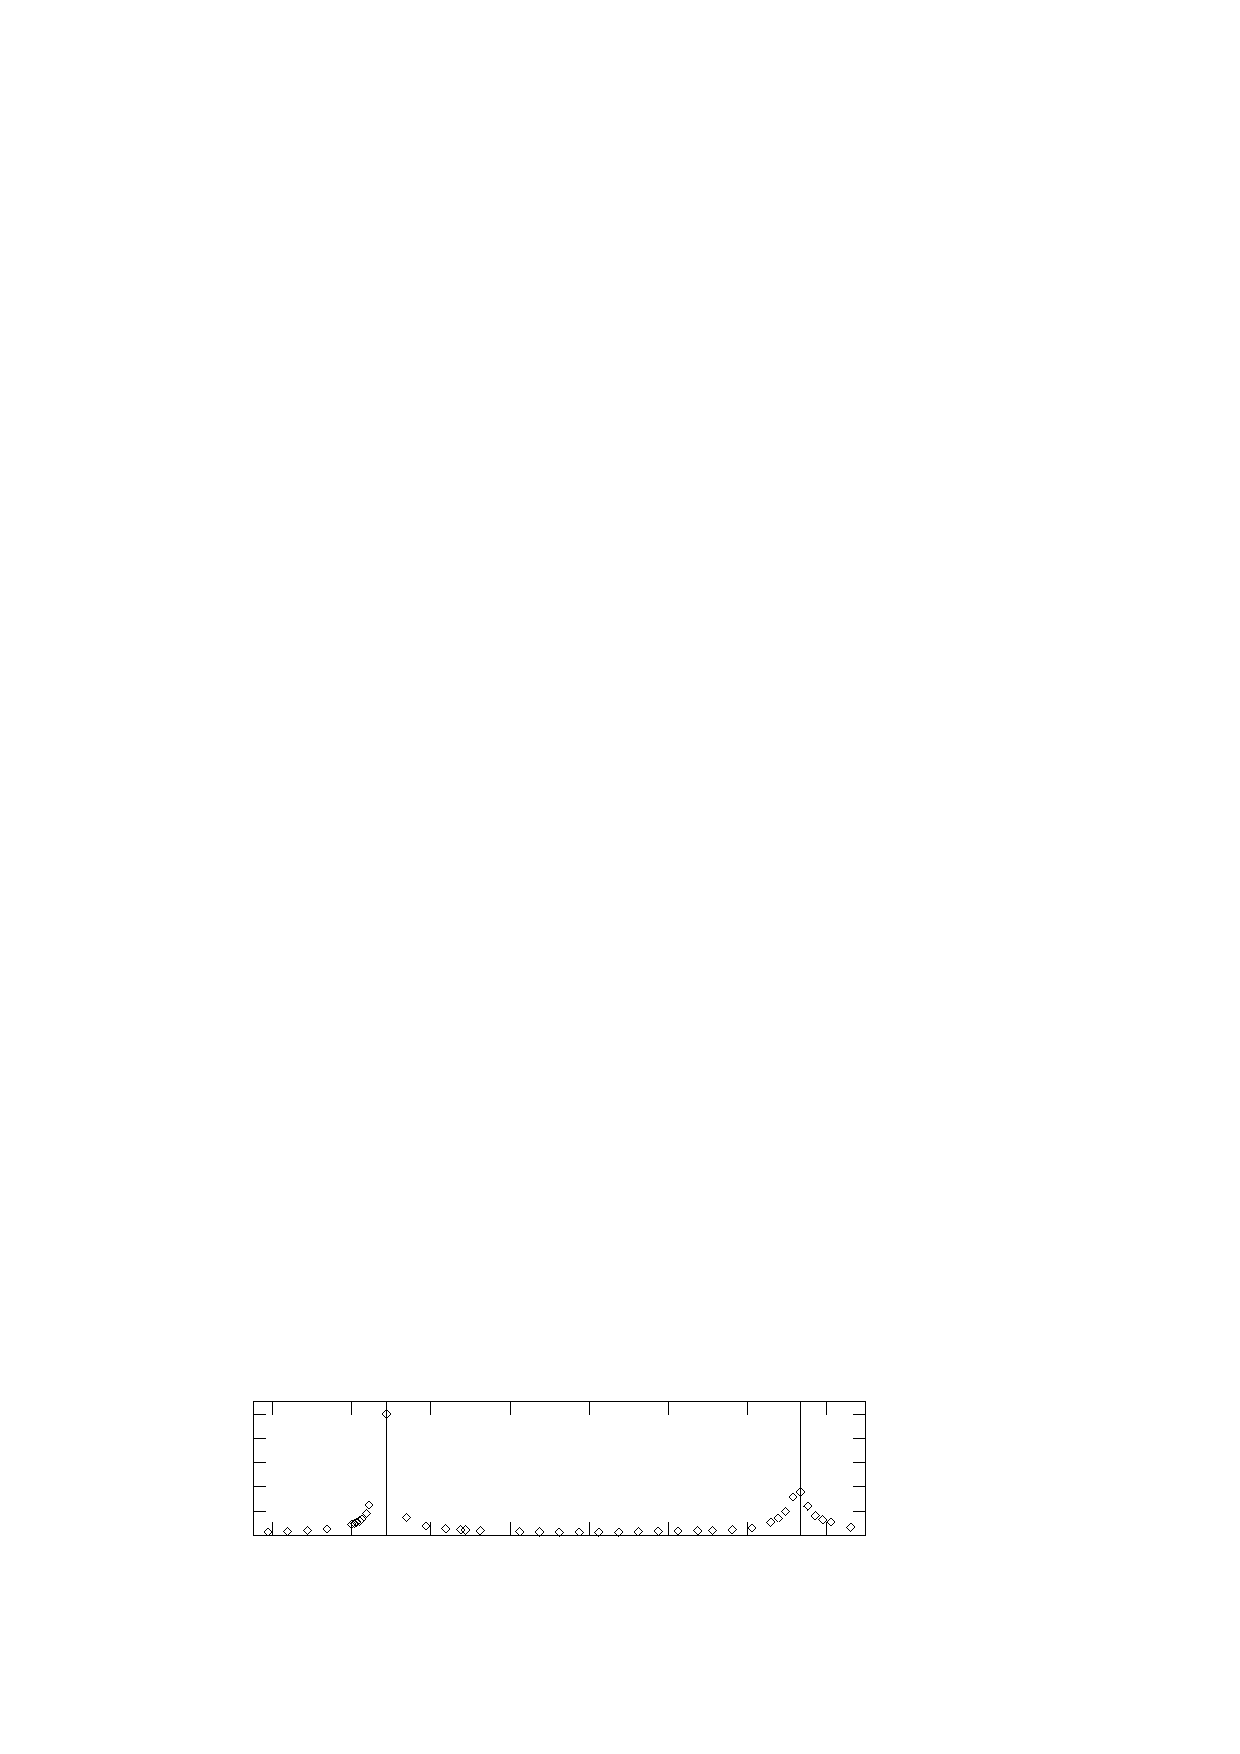
\includegraphics{eps/resonancia}%
\end{picture}%
\begingroup
\setlength{\unitlength}{0.0200bp}%
\begin{picture}(18000,5400)(0,0)%
\put(2200,1650){\makebox(0,0)[r]{\strut{} 0.0}}%
\put(2200,2232){\makebox(0,0)[r]{\strut{} 0.2}}%
\put(2200,2814){\makebox(0,0)[r]{\strut{} 0.4}}%
\put(2200,3395){\makebox(0,0)[r]{\strut{} 0.6}}%
\put(2200,3977){\makebox(0,0)[r]{\strut{} 0.8}}%
\put(2200,4559){\makebox(0,0)[r]{\strut{} 1.0}}%
\put(2949,1100){\makebox(0,0){\strut{} 0.8}}%
\put(4846,1100){\makebox(0,0){\strut{} 1.0}}%
\put(6743,1100){\makebox(0,0){\strut{} 1.2}}%
\put(8640,1100){\makebox(0,0){\strut{} 1.4}}%
\put(10536,1100){\makebox(0,0){\strut{} 1.6}}%
\put(12433,1100){\makebox(0,0){\strut{} 1.8}}%
\put(14330,1100){\makebox(0,0){\strut{} 2.0}}%
\put(16227,1100){\makebox(0,0){\strut{} 2.2}}%
\put(550,3250){\rotatebox{90}{\makebox(0,0){\strut{}$v_{max}/v_1$}}}%
\put(9825,275){\makebox(0,0){\strut{}$H^{\ast}/\pi$}}%
\end{picture}%
\endgroup
\endinput

\caption{\label{fig:resonancia}
Velocidad m'axima adimensional como funci'on de la altura adimensional de la cavidad redondeada.  Las 
velocidades se escalan con la velocidad m'axima del primer modo resonante $v_1$. Los m'aximos se encuentran
en  $H^\ast/\pi =1.09$ y $2.14$.}
\end{figure}

\begin{figure}
%\put(7200,1206){\makebox(0,0){\strut{} $x^\ast$}}%
%\put(4087,4289){\makebox(0,0)[r]{\strut{} $y^\ast$}}%
%\put(7200,206){\makebox(0,0){\strut{} (a)}}%
\hskip -3cm
%GNUPLOT: LaTeX picture with Postscript
%\begin{picture}(0,0)%
%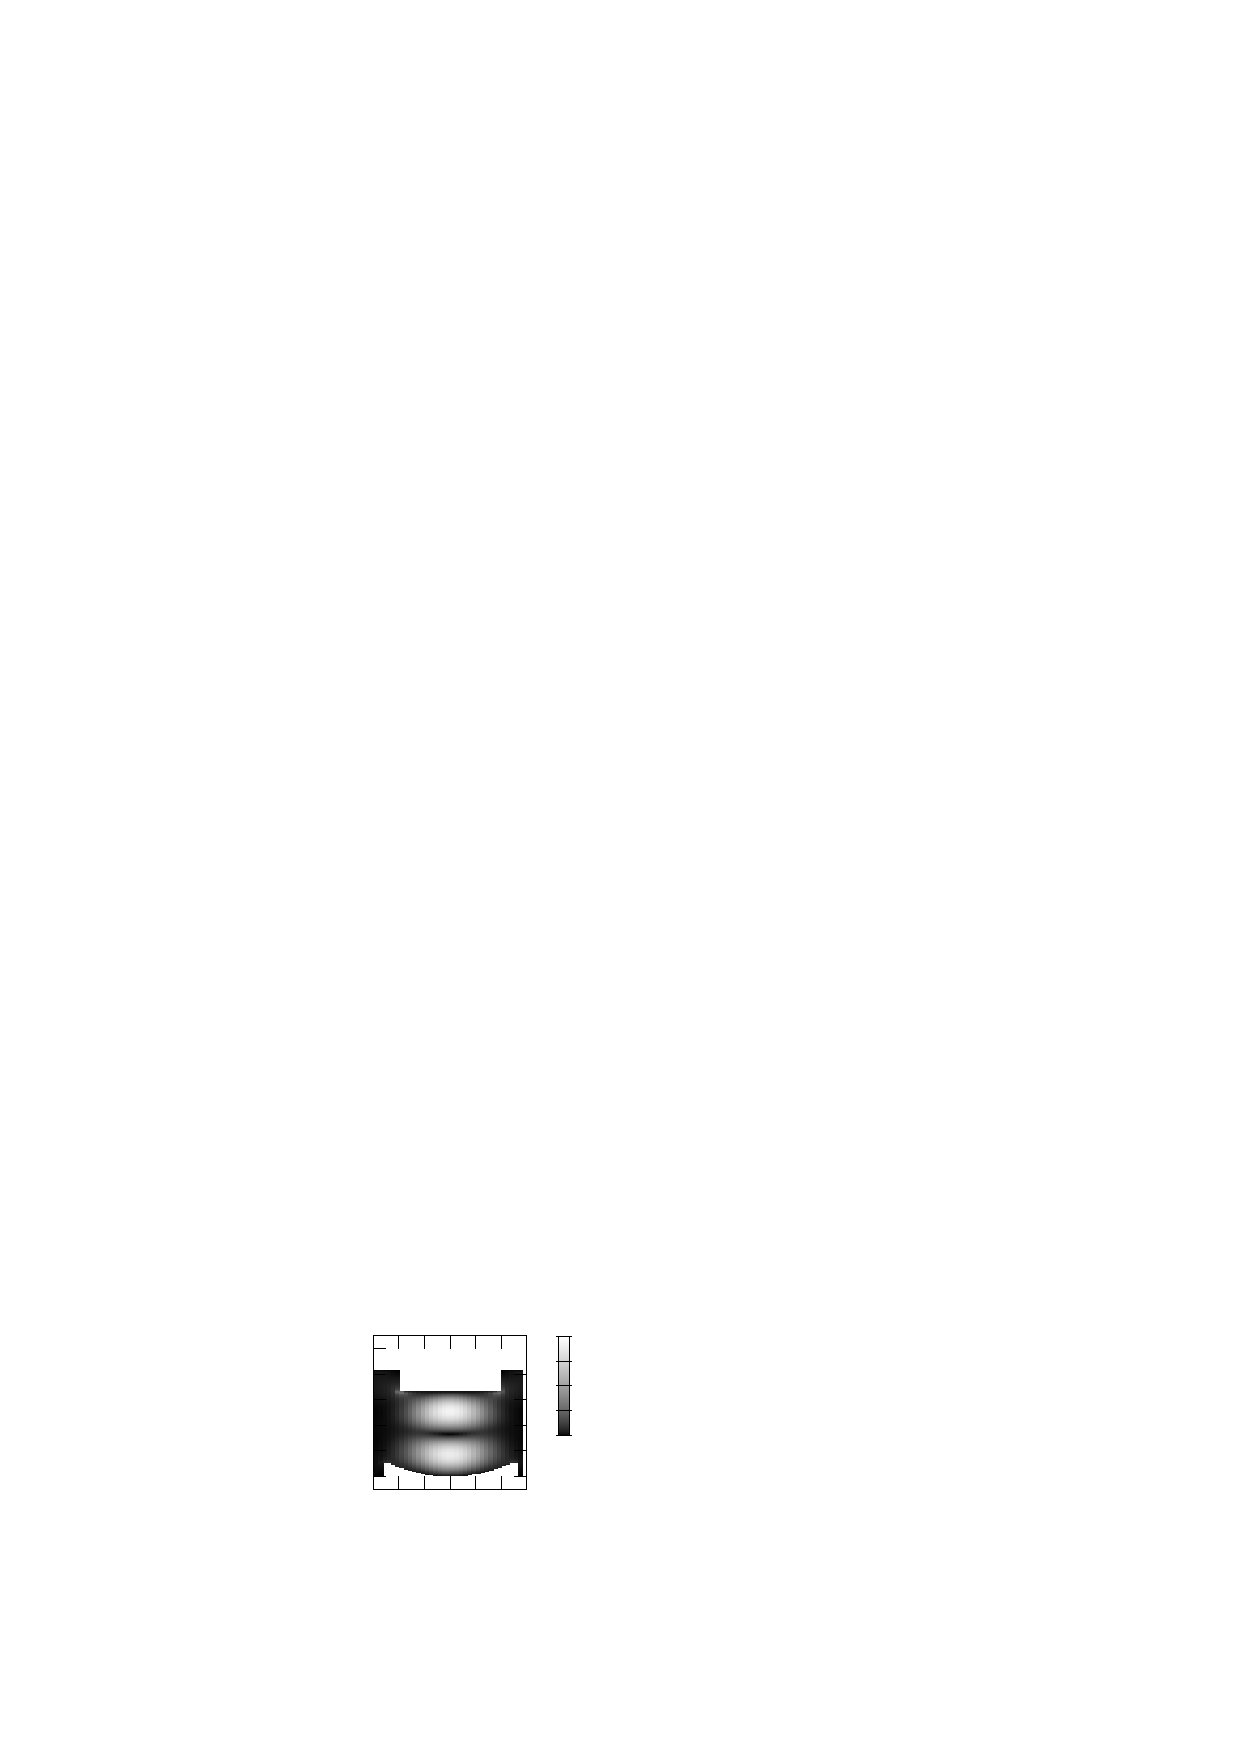
\includegraphics{variaciones-U}%
%\end{picture}%
%\begingroup
%\setlength{\unitlength}{0.0200bp}%
%\begin{picture}(14400,8640)(0,0)%
%\put(10336,4054){\makebox(0,0)[l]{\strut{}0.00}}%
%\put(10336,4646){\makebox(0,0)[l]{\strut{}0.25}}%
%\put(10336,5238){\makebox(0,0)[l]{\strut{}0.50}}%
%\put(10336,5830){\makebox(0,0)[l]{\strut{}0.75}}%
%\put(10336,6422){\makebox(0,0)[l]{\strut{}1.00}}%
%\put(9038,2206){\makebox(0,0){\strut{}-6}}%
%\put(8426,2206){\makebox(0,0){\strut{}-4}}%
%\put(7812,2206){\makebox(0,0){\strut{}-2}}%
%\put(7200,2206){\makebox(0,0){\strut{} 0}}%
%\put(6587,2206){\makebox(0,0){\strut{} 2}}%
%\put(5974,2206){\makebox(0,0){\strut{} 4}}%
%\put(5361,2206){\makebox(0,0){\strut{} 6}}%
%\put(5086,3063){\makebox(0,0)[r]{\strut{} 0}}%
%\put(5086,3676){\makebox(0,0)[r]{\strut{} 2}}%
%\put(5087,4289){\makebox(0,0)[r]{\strut{} 4}}%
%\put(5087,4901){\makebox(0,0)[r]{\strut{} 6}}%
%\put(5087,5514){\makebox(0,0)[r]{\strut{} 8}}%
%\put(5087,6127){\makebox(0,0)[r]{\strut{} 10}}%
%\put(7200,1206){\makebox(0,0){\strut{} $x^\ast$}}%
%\put(4087,4289){\makebox(0,0)[r]{\strut{} $y^\ast$}}%
%\put(7200,206){\makebox(0,0){\strut{} (a)}}%
%\end{picture}%
%\endgroup
%\endinput

\hskip -3.1cm
%GNUPLOT: LaTeX picture with Postscript
%\begin{picture}(0,0)%
%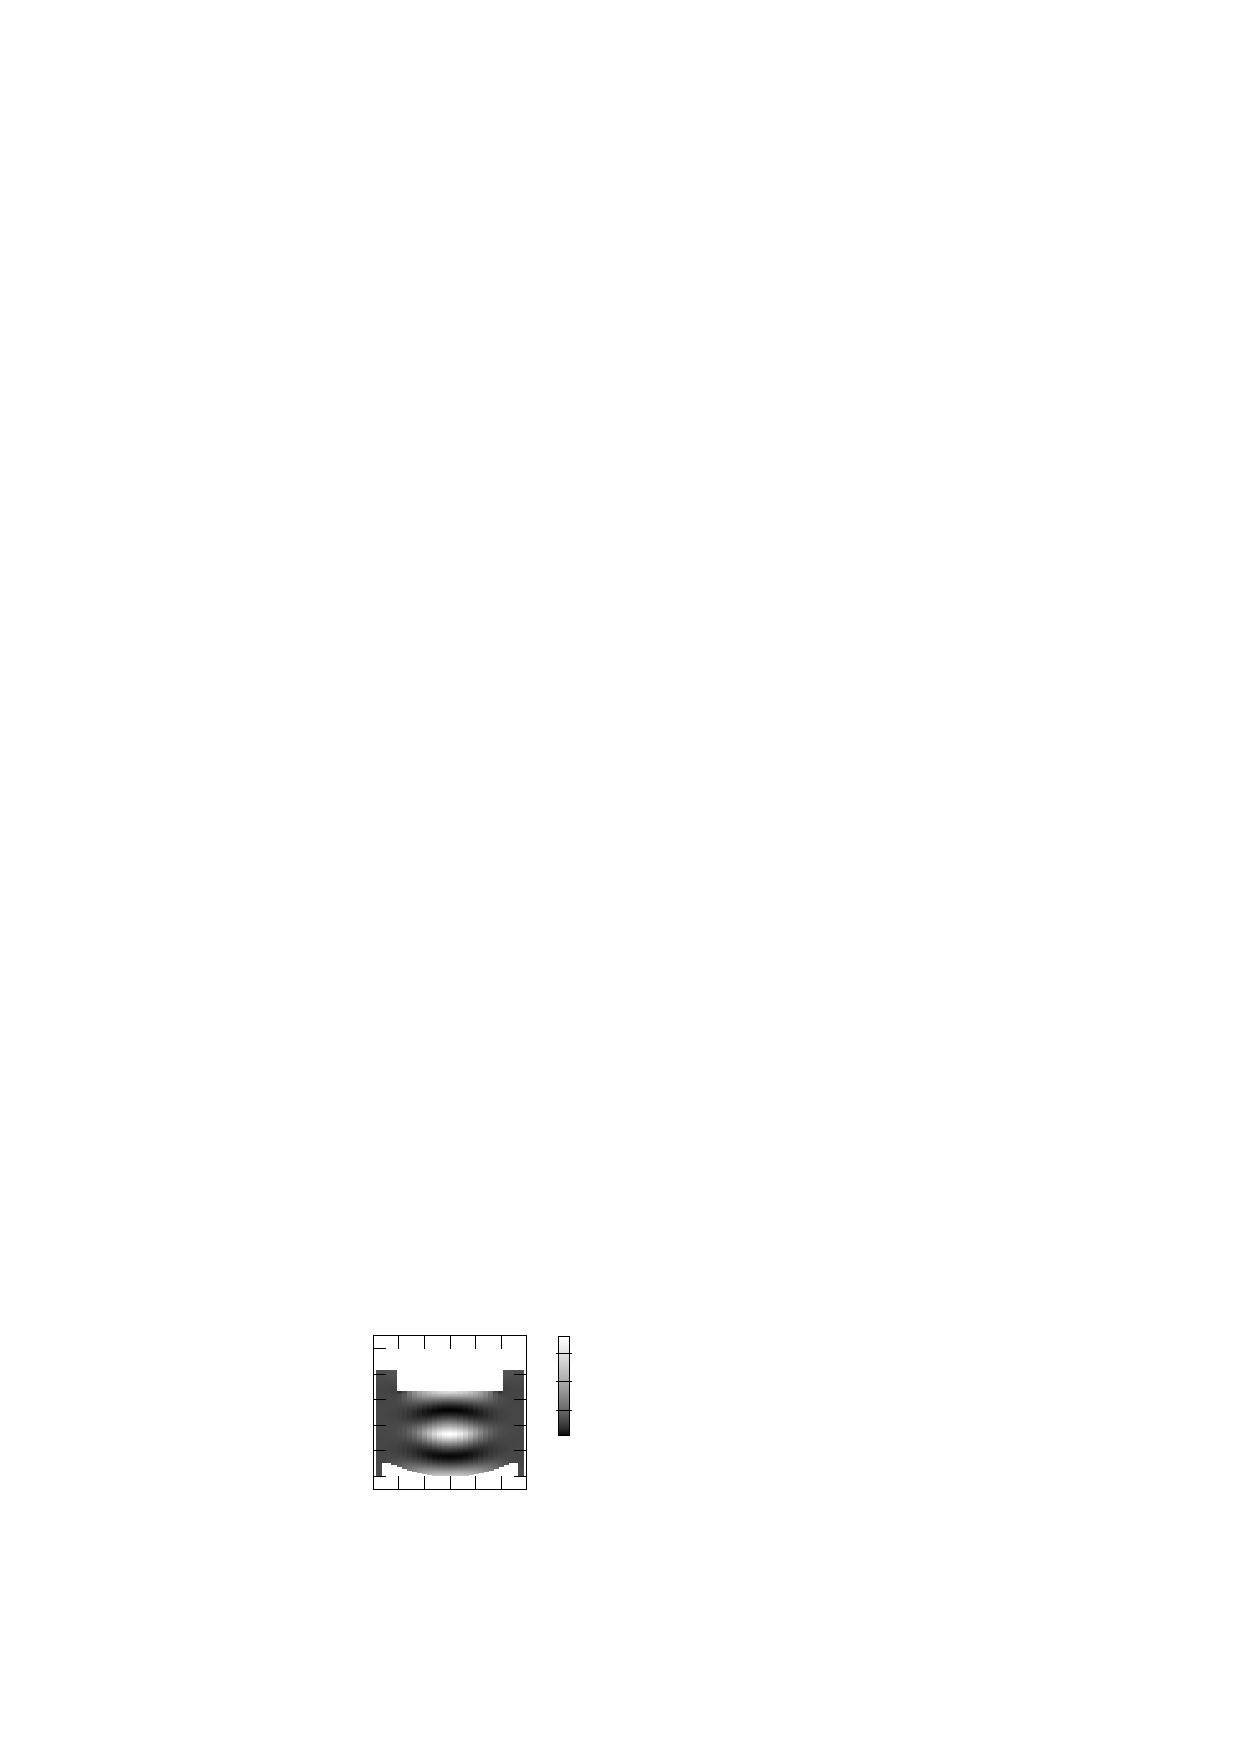
\includegraphics{variaciones-P}%
%\end{picture}%
%\begingroup
%\setlength{\unitlength}{0.0200bp}%
%\begin{picture}(14400,8640)(0,0)%
%\put(10336,4643){\makebox(0,0)[l]{\strut{}1.001}}%
%\put(10336,5329){\makebox(0,0)[l]{\strut{}1.003}}%
%\put(10336,6015){\makebox(0,0)[l]{\strut{}1.005}}%
%\put(9038,2206){\makebox(0,0){\strut{}-6}}%
%\put(8426,2206){\makebox(0,0){\strut{}-4}}%
%\put(7812,2206){\makebox(0,0){\strut{}-2}}%
%\put(7200,2206){\makebox(0,0){\strut{} 0}}%
%\put(6587,2206){\makebox(0,0){\strut{} 2}}%
%\put(5974,2206){\makebox(0,0){\strut{} 4}}%
%\put(5361,2206){\makebox(0,0){\strut{} 6}}%
%\put(5086,3063){\makebox(0,0)[r]{\strut{} 0}}%
%\put(5086,3676){\makebox(0,0)[r]{\strut{} 2}}%
%\put(5087,4289){\makebox(0,0)[r]{\strut{} 4}}%
%\put(5087,4901){\makebox(0,0)[r]{\strut{} 6}}%
%\put(5087,5514){\makebox(0,0)[r]{\strut{} 8}}%
%\put(5087,6127){\makebox(0,0)[r]{\strut{} 10}}%
%\put(7200,1206){\makebox(0,0){\strut{} $x^\ast$}}%
%\put(4087,4289){\makebox(0,0)[r]{\strut{} $y^\ast$}}%
%\put(7200,206){\makebox(0,0){\strut{} (b)}}%
%\end{picture}%
%\endgroup
%\endinput

\caption{\label{fig:nodos-presion-velocidad}
(a) Amplitud de la oscilaci'on de la velocidad escalada con la velocidad m'axima y (b) amplitud de oscilaci'on 
de la presi'on escalada con la presi'on inicial. La cantidad de movimiento agregado por la fuente ac'ustica es 
$P_o^\ast = 1.6 \times 10^{-3}$.
}
\end{figure}



Las siguientes simulaciones num'ericas corresponden al segundo modo resonante para ambas cavidades
y la part'icula s'olida de radio $r^\ast =0.25$ se liber'o a diferentes alturas.  
En las figuras~\ref{fig:nodos-presion-velocidad} (a) y (b) se muestra la amplitud de la oscilaci'on para la velocidad
y la presi'on en la cavidad redondeada, respectivamente. De estas figuras se  observa que a un nodo
de presi'on le corresponde un antinodo de velocidad y viceversa. 
En las figuras~\ref{fig:y-g-0} (a) y (b) se muestra la trayectoria
vertical de la part'icula para la cavidad plana y redondeada, respectivamente. Las part'iculas
presentaron un movimiento en el eje horizontal. La cantidad de movimiento
agregada a la fuente ac'ustica es  $P_o^\ast=1.6 \times 10^{-3}$, $\rho_p/\rho_f =2$ 
y no existe campo gravitacional, por lo que las part'iculas se dirigen al nodo de presi'on, 
donde la sumatoria de fuerzas ac'usticas es cero. De estas figuras, es evidente que a las part'iculas liberadas
en la cavidad redondeada alcanzaron su posici'on de equilibrio en menos tiempo que las liberadas
en la cavidad plana, adem'as  la oscilaci'on de la part'icula alrededor de su posici'on
de equilibrio es tambi'en m'as grande en la cavidad redondeada que en la plana para la misma cantidad de 
movimiento agregada por la fuente ac'ustica.
\begin{figure}
%\put(7650,9588){\makebox(0,0)[r]{\strut{} (a)}}%
%%GNUPLOT: LaTeX picture with Postscript
%\begin{picture}(0,0)%
%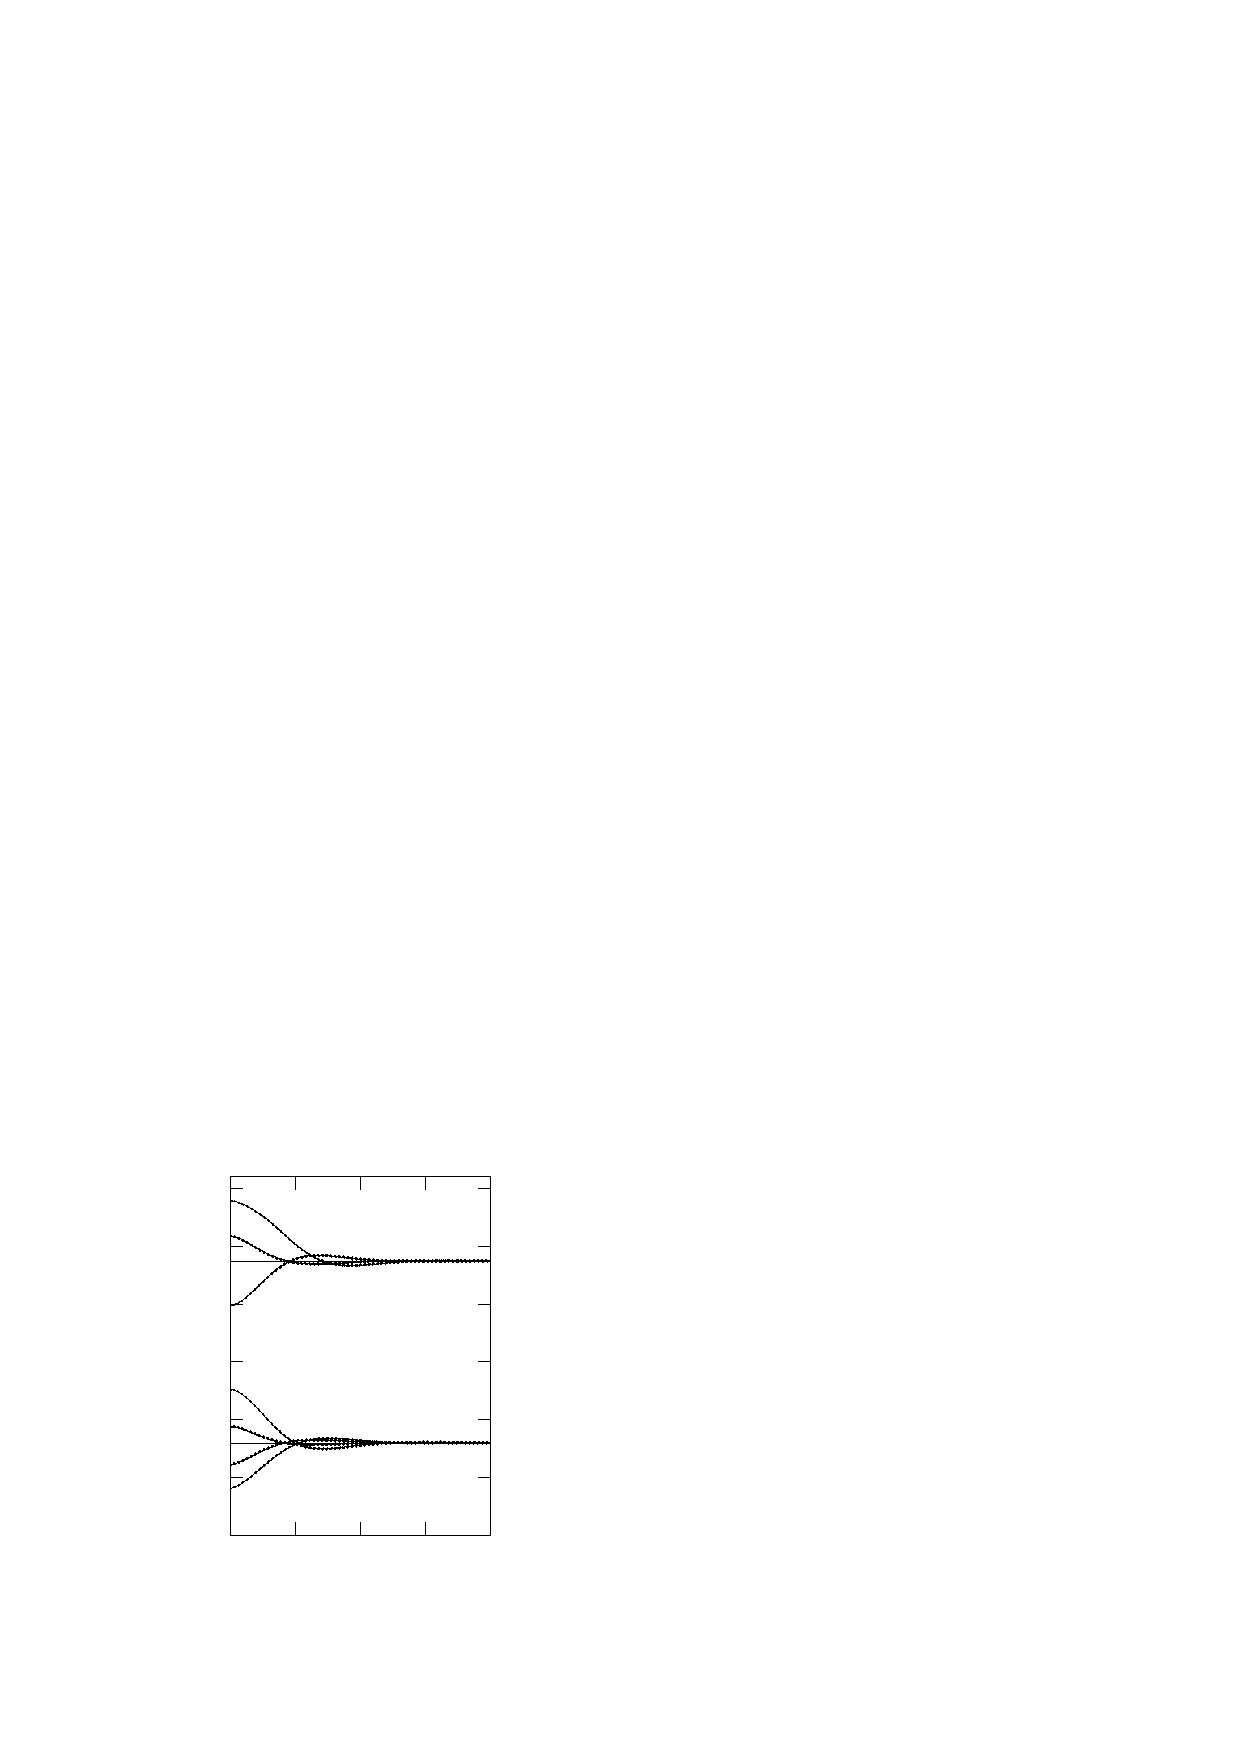
\includegraphics{position-flat-zerogravity}%
%\end{picture}%
%\begingroup
%\setlength{\unitlength}{0.0200bp}%
%\begin{picture}(9000,10800)(0,0)%
%\put(1650,1650){\makebox(0,0)[r]{\strut{} 0}}%
%\put(1650,3037){\makebox(0,0)[r]{\strut{} 1}}%
%\put(1650,4424){\makebox(0,0)[r]{\strut{} 2}}%
%\put(1650,5811){\makebox(0,0)[r]{\strut{} 3}}%
%\put(1650,7198){\makebox(0,0)[r]{\strut{} 4}}%
%\put(1650,8585){\makebox(0,0)[r]{\strut{} 5}}%
%\put(1650,9973){\makebox(0,0)[r]{\strut{} 6}}%
%\put(1925,1100){\makebox(0,0){\strut{} 0}}%
%\put(3488,1100){\makebox(0,0){\strut{} 50}}%
%\put(5050,1100){\makebox(0,0){\strut{} 100}}%
%\put(6613,1100){\makebox(0,0){\strut{} 150}}%
%\put(8175,1100){\makebox(0,0){\strut{} 200}}%
%\put(550,5950){\rotatebox{90}{\makebox(0,0){\strut{}$y^\ast$}}}%
%\put(5050,275){\makebox(0,0){\strut{}$t^\ast$}}%
%\put(7650,9588){\makebox(0,0)[r]{\strut{} (a)}}%
%\end{picture}%
%\endgroup
%\endinput

%GNUPLOT: LaTeX picture with Postscript
\begin{picture}(0,0)%
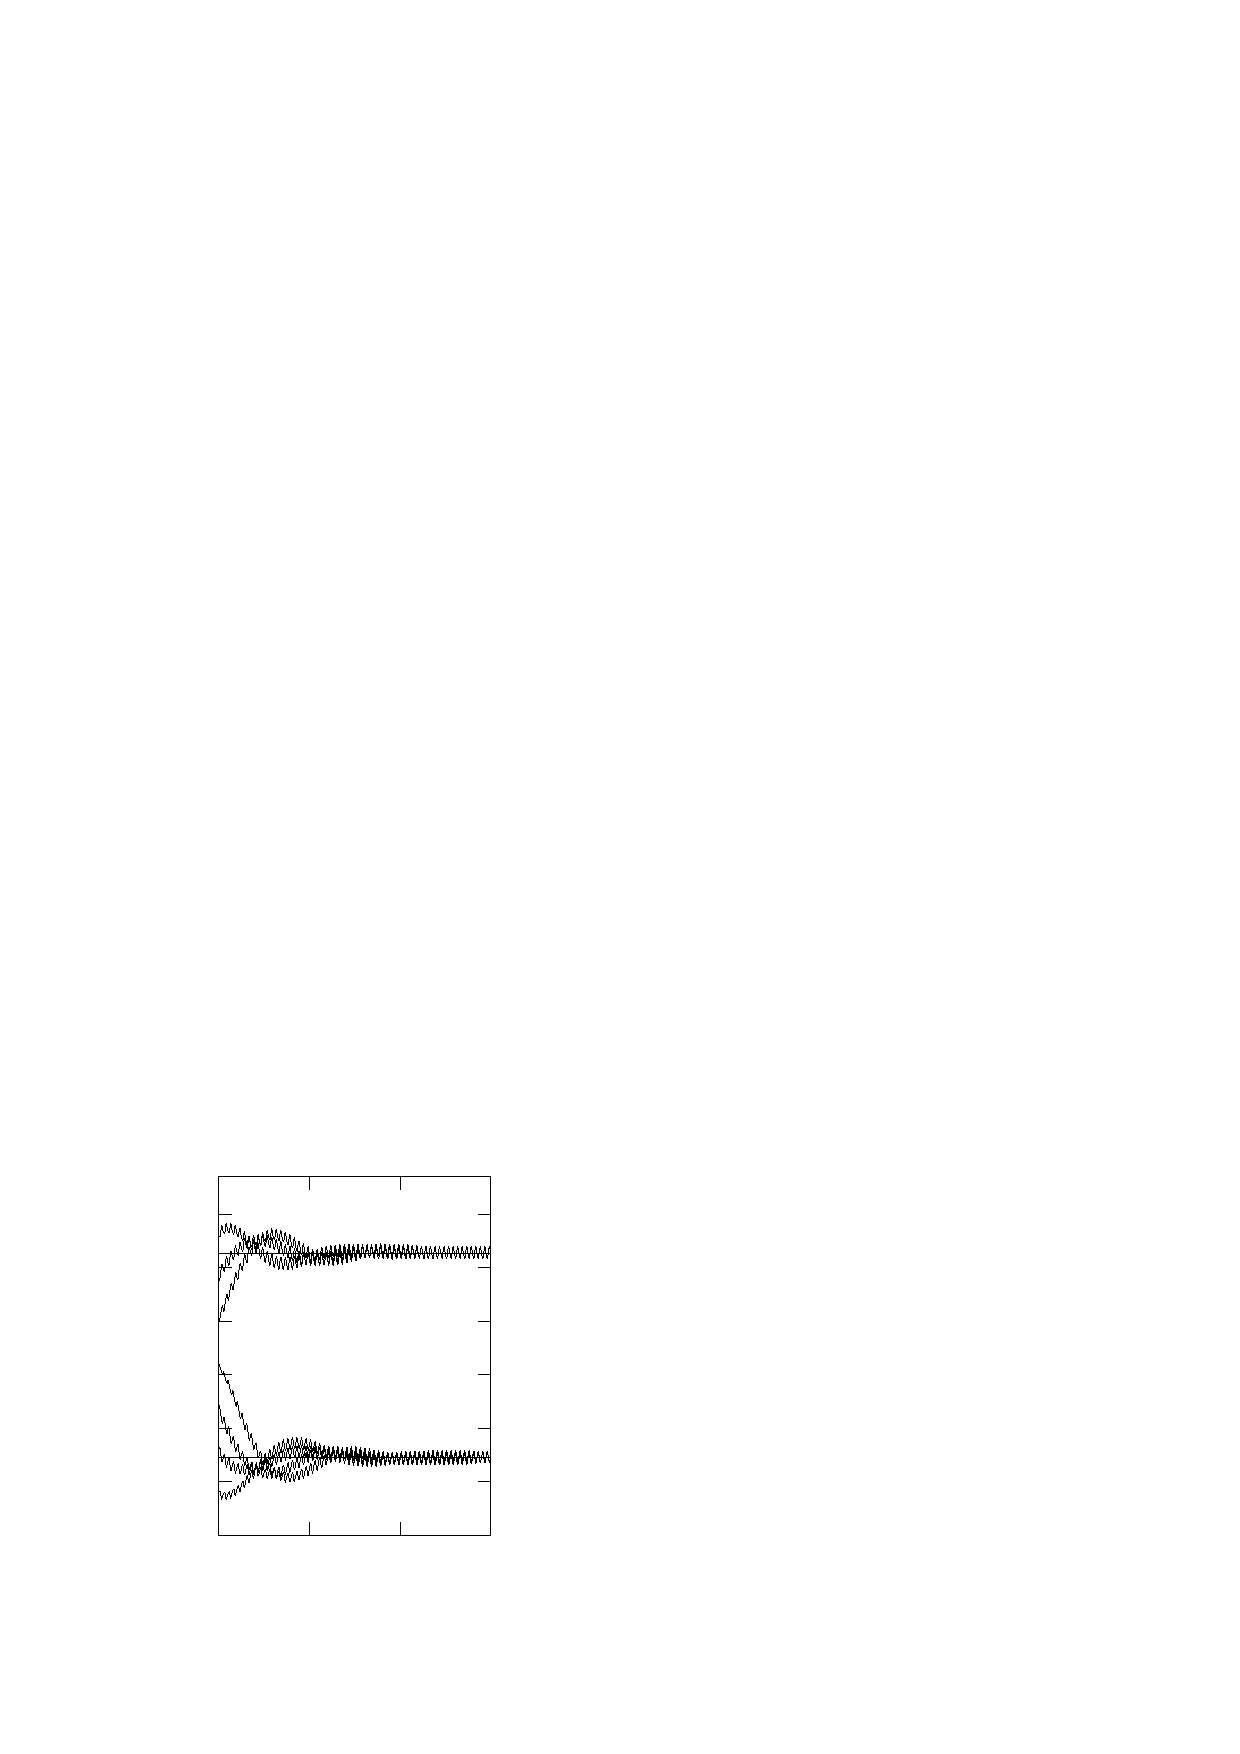
\includegraphics{eps/position-rounded-zerogravity}%
\end{picture}%
\begingroup
\setlength{\unitlength}{0.0200bp}%
\begin{picture}(9000,10800)(0,0)%
\put(1375,1650){\makebox(0,0)[r]{\strut{}0}}%
\put(1375,2934){\makebox(0,0)[r]{\strut{}1}}%
\put(1375,4217){\makebox(0,0)[r]{\strut{}2}}%
\put(1375,5501){\makebox(0,0)[r]{\strut{}3}}%
\put(1375,6784){\makebox(0,0)[r]{\strut{}4}}%
\put(1375,8068){\makebox(0,0)[r]{\strut{}5}}%
\put(1375,9351){\makebox(0,0)[r]{\strut{}6}}%
\put(1650,1100){\makebox(0,0){\strut{} 0}}%
\put(3825,1100){\makebox(0,0){\strut{} 20}}%
\put(6000,1100){\makebox(0,0){\strut{} 40}}%
\put(8175,1100){\makebox(0,0){\strut{} 60}}%
\put(550,5950){\rotatebox{90}{\makebox(0,0){\strut{}$y^\ast$}}}%
\put(4912,275){\makebox(0,0){\strut{}$t^\ast$}}%

\put(7650,9588){\makebox(0,0)[r]{\strut{} (b)}}%

\end{picture}%
\endgroup
\endinput

\vskip 5mm
\caption{\label{fig:y-g-0}
Evoluci'on de la posici'on vertical de una part'icula s'olida como funci'on del tiempo
en el segundo modo resonante en ausencia de gravedad en (a) la cavidad  plana y (b) la
cavidad  redondeada, ambas con  $P_o^\ast = 1.6\times 10^{-3}$, $\rho_p/\rho_f=2$, y $r^\ast=0.25$.
Las l'ineas horizontales representan la ubicaci'on de los nodos de presi'on. 
Se usaron mallas de  $163\times 201$ y $901\times 253$ para la cavidad plana y la redondeada, respectivamente.
}
\end{figure}
\begin{figure}
%\put(3250,4283){\makebox(0,0){\strut{} (a)}}%
%\put(3250,4283){\makebox(0,0){\strut{} (b)}}%
%GNUPLOT: LaTeX picture with Postscript
%\begin{picture}(0,0)%
%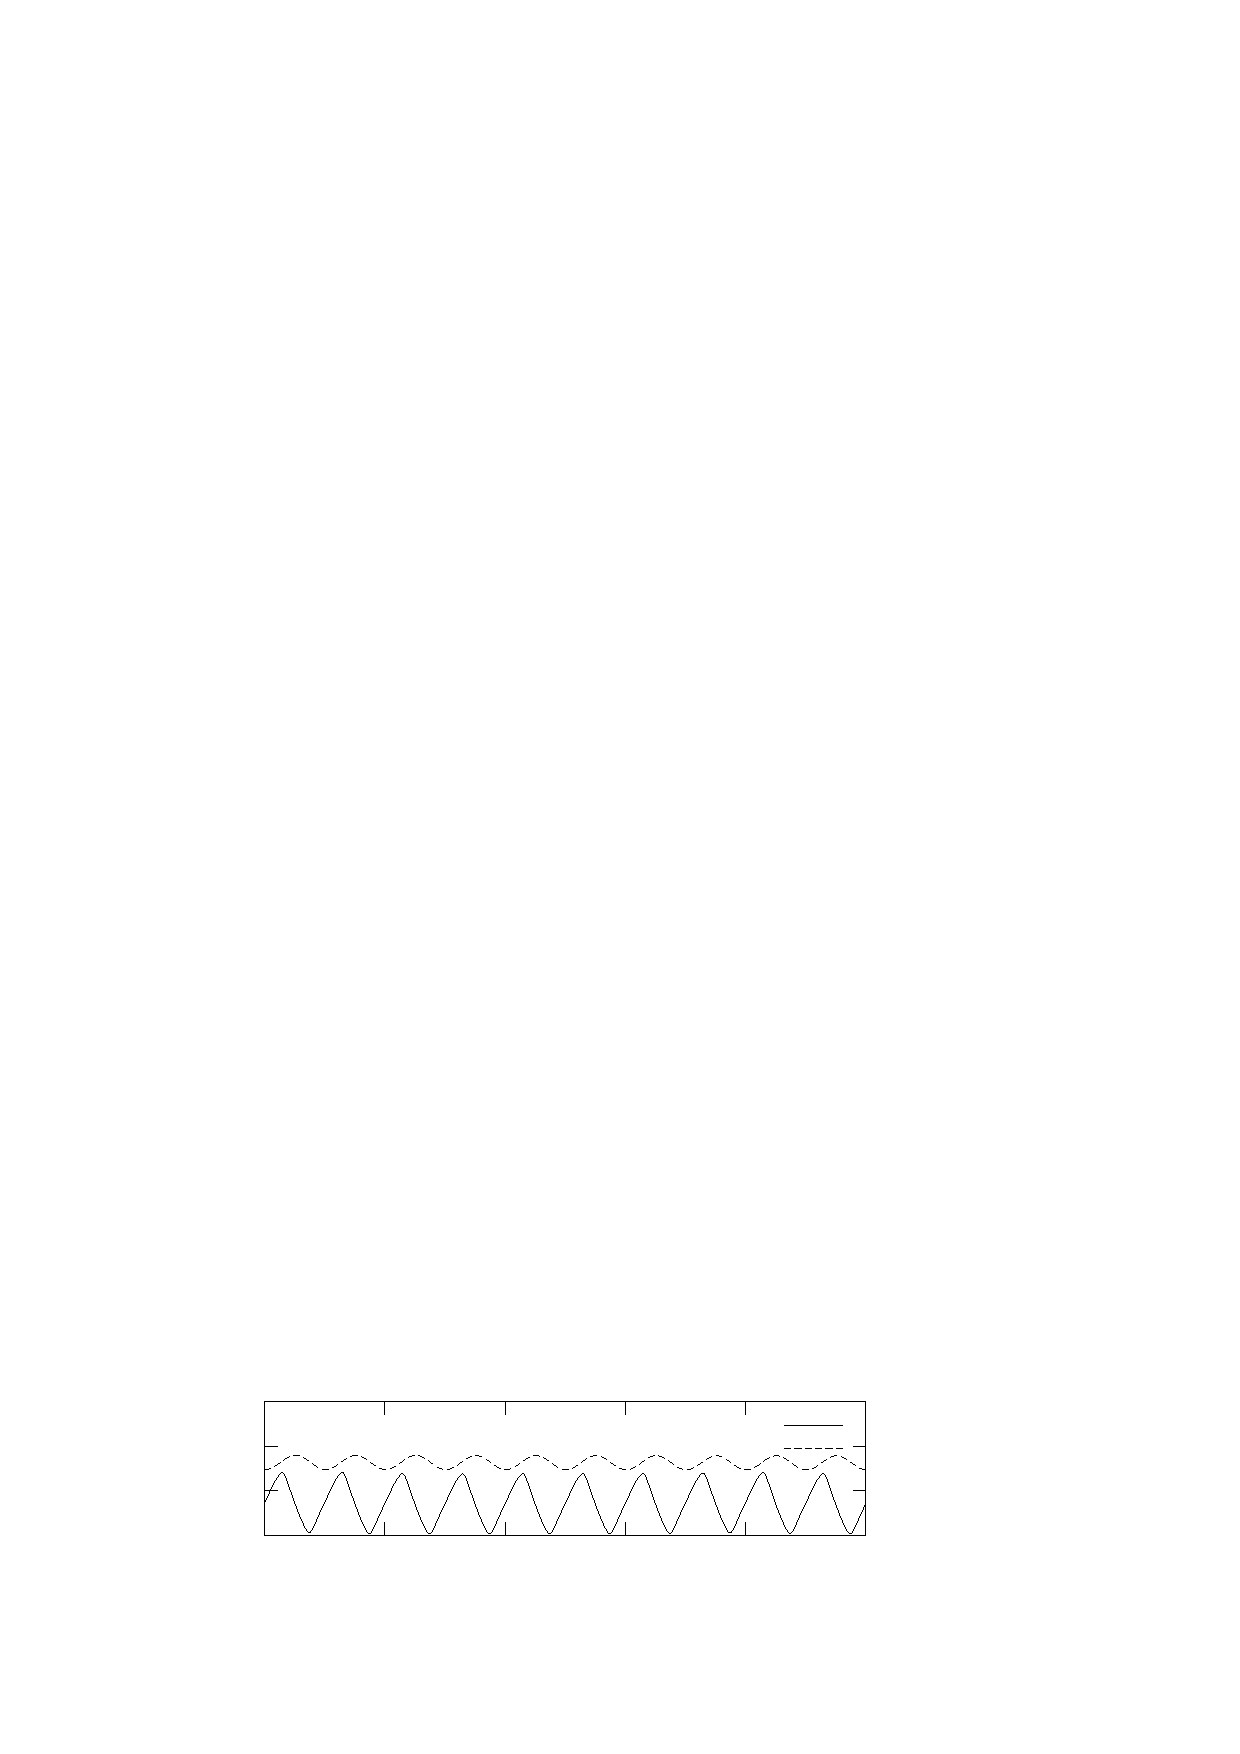
\includegraphics{detalle-rounded-flat-zerogravity}%
%\end{picture}%
%\begingroup
%\setlength{\unitlength}{0.0200bp}%
%\begin{picture}(18000,5400)(0,0)%
%\put(2475,1650){\makebox(0,0)[r]{\strut{} 1.35}}%
%\put(2475,2717){\makebox(0,0)[r]{\strut{} 1.50}}%
%\put(2475,3783){\makebox(0,0)[r]{\strut{} 1.65}}%
%\put(2475,4850){\makebox(0,0)[r]{\strut{} 1.80}}%
%\put(2750,1100){\makebox(0,0){\strut{} 120}}%
%\put(5635,1100){\makebox(0,0){\strut{} 122}}%
%\put(8520,1100){\makebox(0,0){\strut{} 124}}%
%\put(11405,1100){\makebox(0,0){\strut{} 126}}%
%\put(14290,1100){\makebox(0,0){\strut{} 128}}%
%\put(17175,1100){\makebox(0,0){\strut{} 130}}%
%\put(550,3250){\rotatebox{90}{\makebox(0,0){\strut{}$y^\ast$}}}%
%\put(9962,275){\makebox(0,0){\strut{}$t^\ast$}}%
%%\put(600,1000){\rotatebox{0}{\makebox(0,0){\strut{}(a)}}}%
%\put(14950,4275){\makebox(0,0)[r]{\strut{}redondeada}}%
%\put(14950,3725){\makebox(0,0)[r]{\strut{}plana}}%
%\end{picture}%
%\endgroup
%\endinput

%GNUPLOT: LaTeX picture with Postscript
\begin{picture}(0,0)%
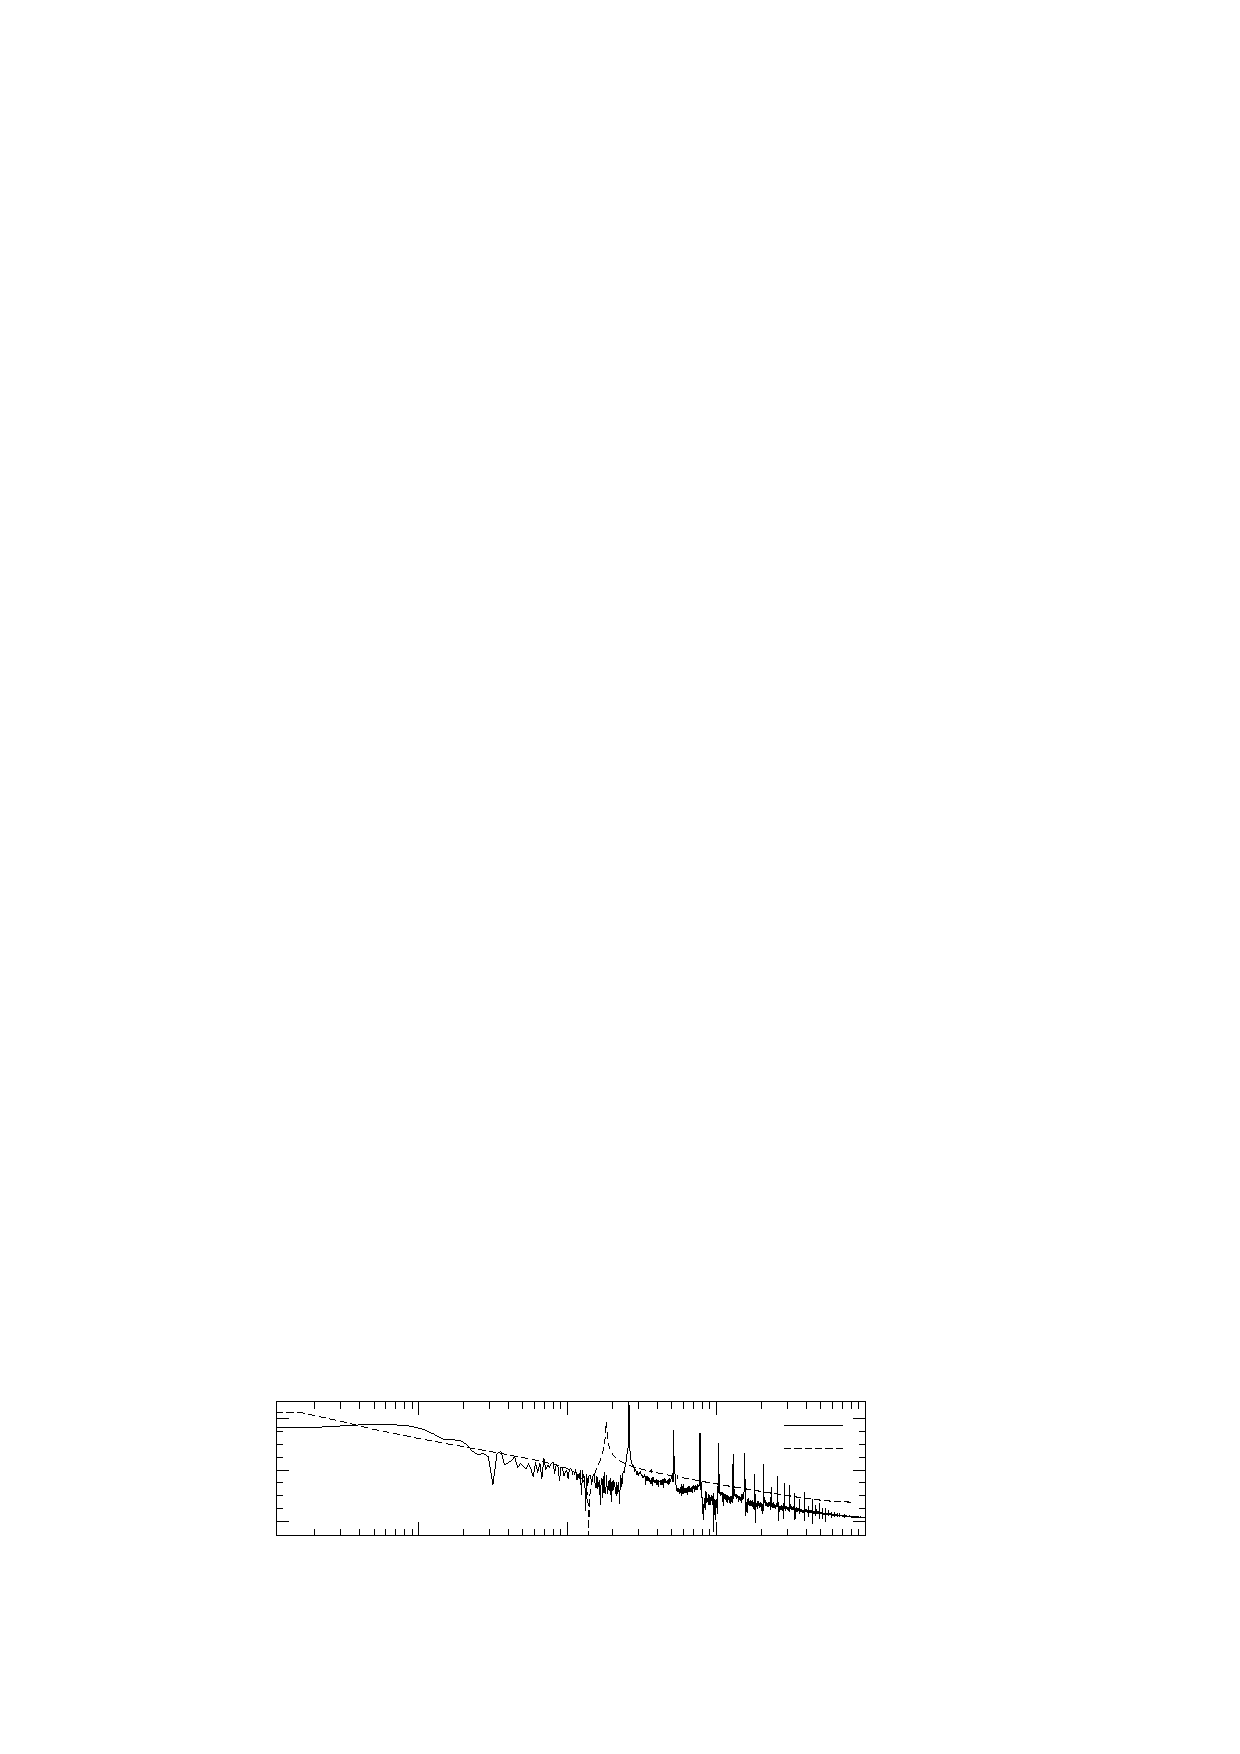
\includegraphics{detalle-frecuencias-rounded-flat}%
\end{picture}%
\begingroup
\setlength{\unitlength}{0.0200bp}%
\begin{picture}(18000,5400)(0,0)%
\put(2750,1987){\makebox(0,0)[r]{\strut{} 1e-12}}%
\put(2750,3214){\makebox(0,0)[r]{\strut{} 1e-08}}%
\put(2750,4441){\makebox(0,0)[r]{\strut{} 1e-04}}%
\put(6452,1100){\makebox(0,0){\strut{} 0.001}}%
\put(10026,1100){\makebox(0,0){\strut{} 0.01}}%
\put(13601,1100){\makebox(0,0){\strut{} 0.1}}%
\put(17175,1100){\makebox(0,0){\strut{} 1}}%
\put(550,3250){\rotatebox{90}{\makebox(0,0){\strut{}$PSD$}}}%
\put(10100,275){\makebox(0,0){\strut{}$\omega$}}%
\put(14950,4275){\makebox(0,0)[r]{\strut{}redondeada}}%
\put(14950,3725){\makebox(0,0)[r]{\strut{}plana}}%
\put(600,1000){\rotatebox{0}{\makebox(0,0){\strut{}(b)}}}%
\end{picture}%
\endgroup
\endinput

\caption{\label{fig:detalle-flat-rounded}
(a) Detalle del movimiento de la part'icula para la cavidad
plana y la redondeada, (b) espectro de potencia ($PSD$, por sus siglas en ingl'es) de 
las trayectorias mostradas en (a) para conocer su frecuencia, $\omega_p=0.018138$ para
la part'icula en la cavidad plana y $\omega_r=0.019126$ para la part'icula en la cavidad
redondeada, que corresponden con las frecuencias de la fuente ac'ustica respectivamente.
}
\end{figure}
En la figura~\ref{fig:detalle-flat-rounded} (a), detalle del movimiento de la part'icula en ambas
cavidades, se observa que el movimiento de la part'icula s'olida sigue una trayectoria oscilatoria, donde
la frecuencia  de oscilaci'on es la correspondiente a la frecuencia de la fuente ac'ustica, como se confirma de la 
figura~\ref{fig:detalle-flat-rounded} (b), que es el espectro de potencia de la trayectoria. 
Los picos de esta figura indican las frecuencias dominantes son
$\omega_p=0.018138$ para la part'icula en la cavidad plana y $\omega_r=0.019126$ para la part'icula en la cavidad
redondeada. Tambi'en se observa que el movimiento de la part'icula en la cavidad redondeada presenta arm'onicos
de la frecuencia de la fuente ac'ustica, los cuales no se presentan para la part'icula en la cavidad plana.

\begin{figure}
%\put(7650,9588){\makebox(0,0)[r]{\strut{} (a)}}%
%GNUPLOT: LaTeX picture with Postscript
\begin{picture}(0,0)%
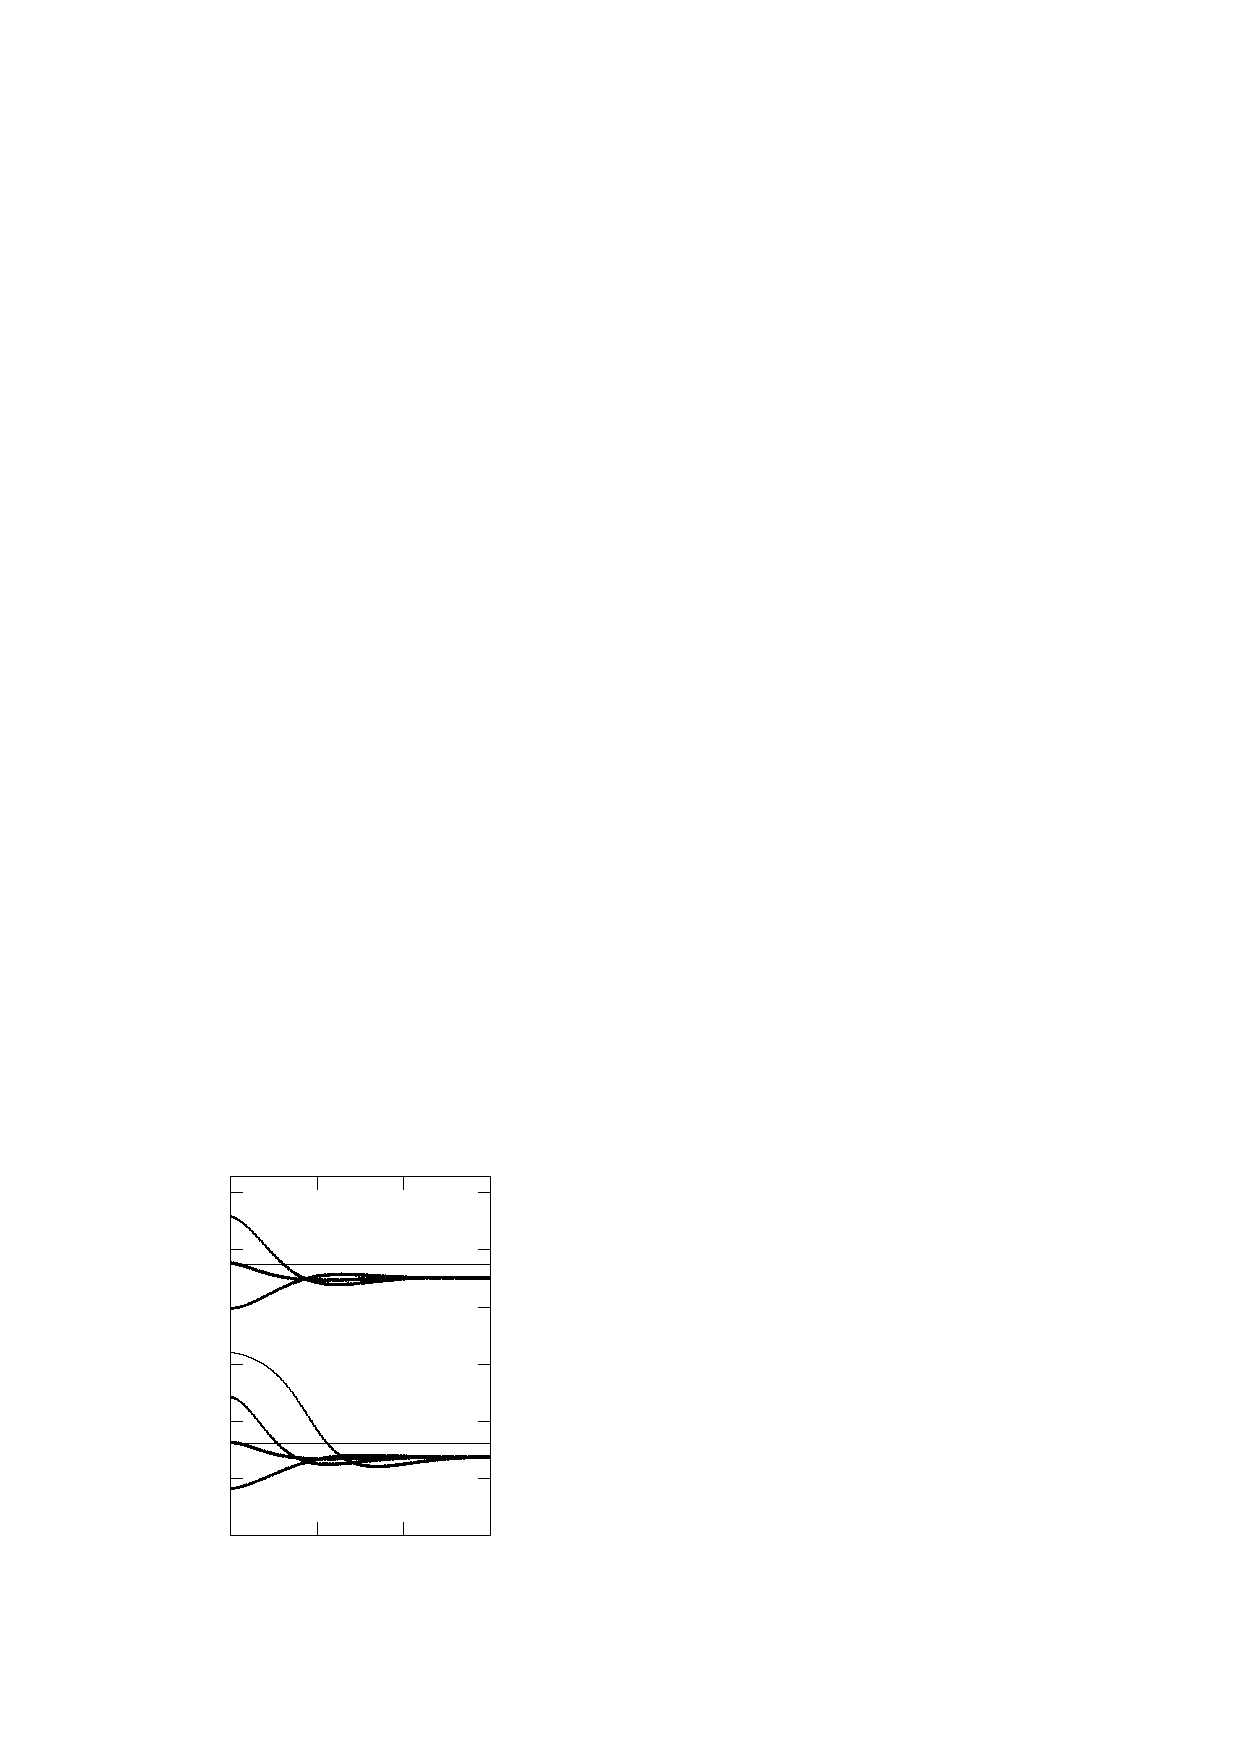
\includegraphics{eps/position-flat-nonzerogravity}%
\end{picture}%
\begingroup
\setlength{\unitlength}{0.0200bp}%
\begin{picture}(9000,10800)(0,0)%
\put(1650,1650){\makebox(0,0)[r]{\strut{} 0}}%
\put(1650,3019){\makebox(0,0)[r]{\strut{} 1}}%
\put(1650,4389){\makebox(0,0)[r]{\strut{} 2}}%
\put(1650,5758){\makebox(0,0)[r]{\strut{} 3}}%
\put(1650,7128){\makebox(0,0)[r]{\strut{} 4}}%
\put(1650,8497){\makebox(0,0)[r]{\strut{} 5}}%
\put(1650,9867){\makebox(0,0)[r]{\strut{} 6}}%
\put(1925,1100){\makebox(0,0){\strut{} 0}}%
\put(4008,1100){\makebox(0,0){\strut{} 60}}%
\put(6092,1100){\makebox(0,0){\strut{} 120}}%
\put(8175,1100){\makebox(0,0){\strut{} 180}}%
\put(550,5950){\rotatebox{90}{\makebox(0,0){\strut{}$y^\ast$}}}%
\put(5050,275){\makebox(0,0){\strut{}$t^\ast$}}%

\put(7650,9588){\makebox(0,0)[r]{\strut{} (a)}}%
\end{picture}%
\endgroup
\endinput

%GNUPLOT: LaTeX picture with Postscript
\begin{picture}(0,0)%
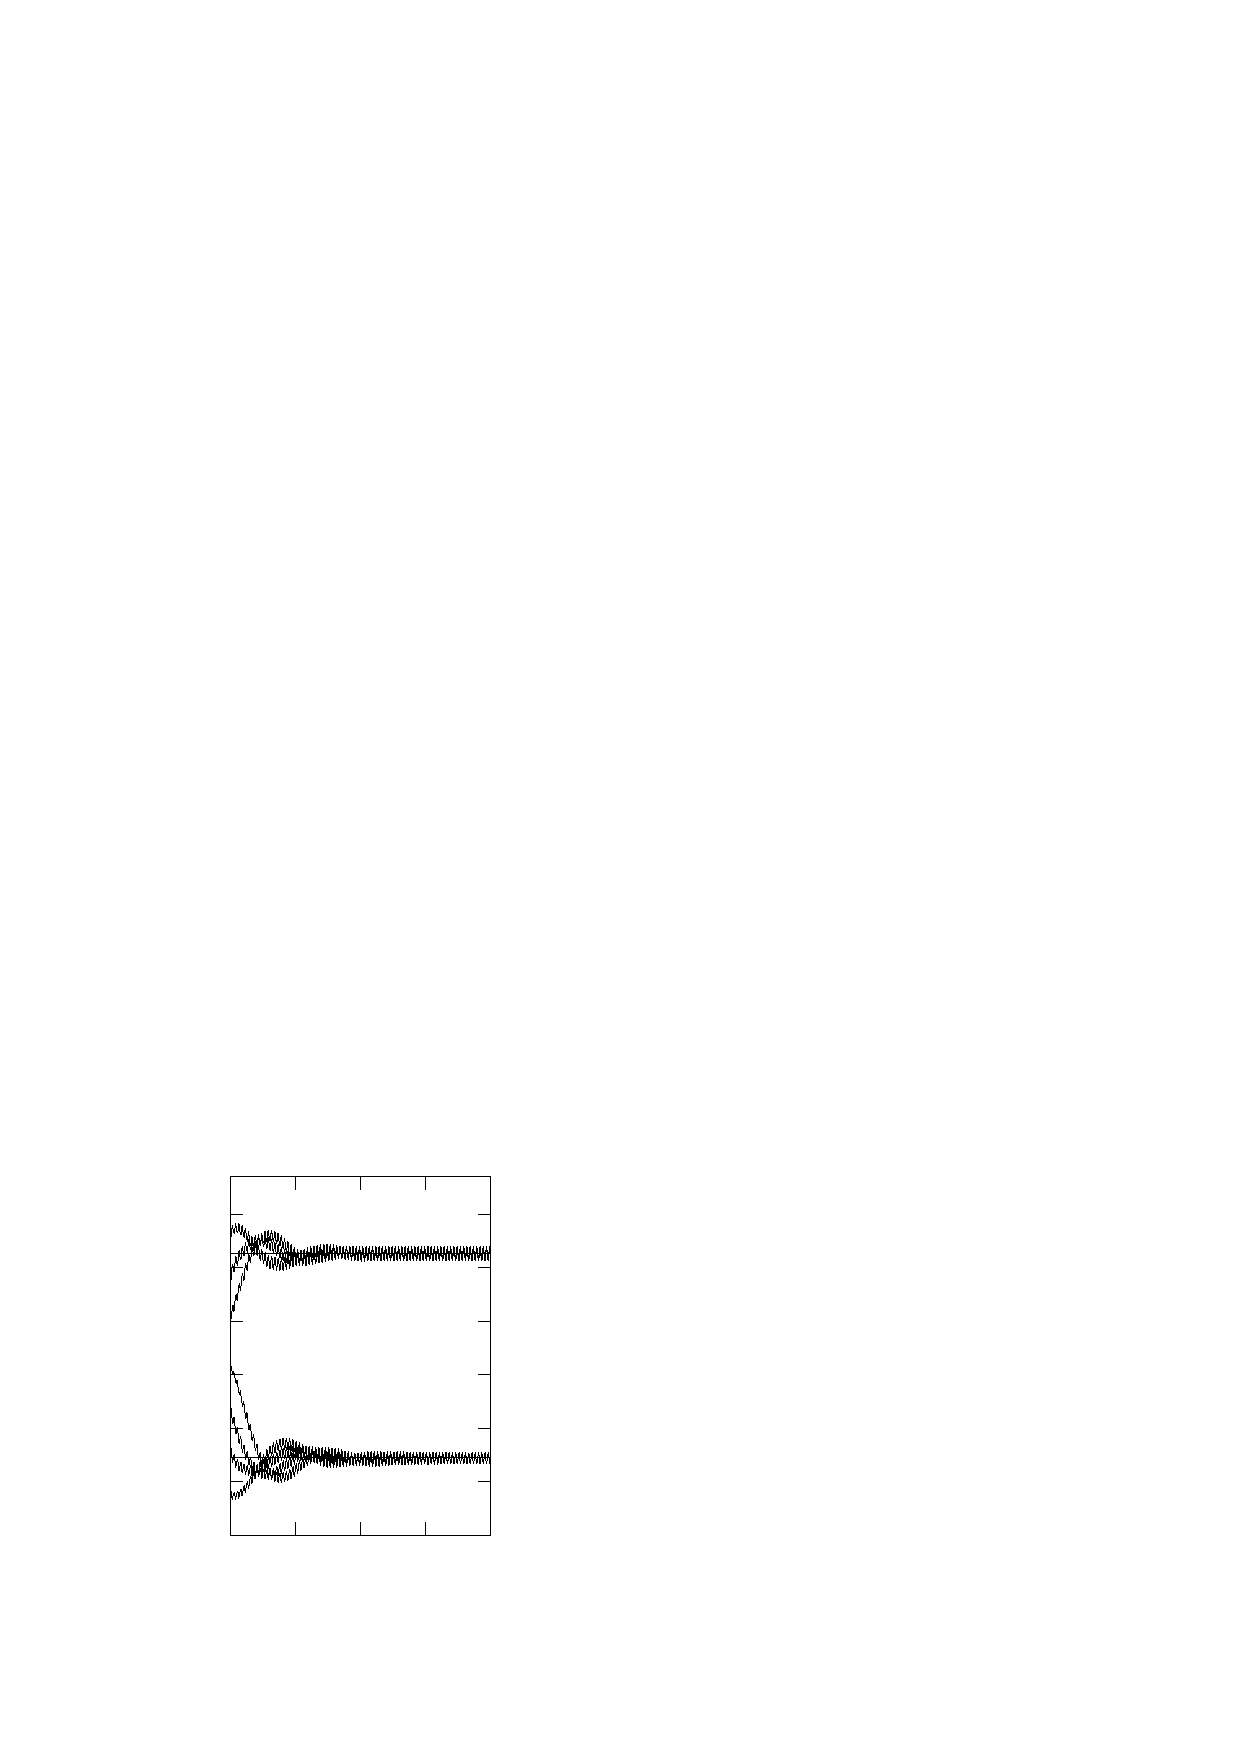
\includegraphics{eps/position-rounded-nonzerogravity}%
\end{picture}%
\begingroup
\setlength{\unitlength}{0.0200bp}%
\begin{picture}(9000,10800)(0,0)%
\put(1650,1650){\makebox(0,0)[r]{\strut{} 0}}%
\put(1650,2934){\makebox(0,0)[r]{\strut{} 1}}%
\put(1650,4217){\makebox(0,0)[r]{\strut{} 2}}%
\put(1650,5501){\makebox(0,0)[r]{\strut{} 3}}%
\put(1650,6784){\makebox(0,0)[r]{\strut{} 4}}%
\put(1650,8068){\makebox(0,0)[r]{\strut{} 5}}%
\put(1650,9351){\makebox(0,0)[r]{\strut{} 6}}%
\put(1925,1100){\makebox(0,0){\strut{} 0}}%
\put(3488,1100){\makebox(0,0){\strut{} 20}}%
\put(5050,1100){\makebox(0,0){\strut{} 40}}%
\put(6613,1100){\makebox(0,0){\strut{} 60}}%
\put(8175,1100){\makebox(0,0){\strut{} 80}}%
\put(550,5950){\rotatebox{90}{\makebox(0,0){\strut{}$y^\ast$}}}%
\put(5050,275){\makebox(0,0){\strut{}$t^\ast$}}%

\put(7650,9588){\makebox(0,0)[r]{\strut{} (b)}}%

\end{picture}%
\endgroup
\endinput

\vskip 5mm
\caption{\label{fig:path-3} 
(a) Trayectoria vertical para una part'icula s'olida liberada a diferentes
alturas en la cavidad plana y
(b)  para la cavidad redondeada, ambas en presencia de un campo gravitacinal externo.
Las l'ineas solidas representan la posici'on vertical de los nodos de presi'on. La posici'on
de equilibrio de la part'icula se desplaza debido a la presencia del campo gravitacional externo.
Las simulaciones num'ericas se realizaron con los mismos par'ametros 
de las figuras~\ref{fig:y-g-0} (a) y (b).
}
\end{figure}
\begin{figure}
%\put(3250,4283){\makebox(0,0){\strut{} (a)}}
%\put(3650,2283){\makebox(0,0){\strut{} (b)}}%
%GNUPLOT: LaTeX picture with Postscript
%\begin{picture}(0,0)%
%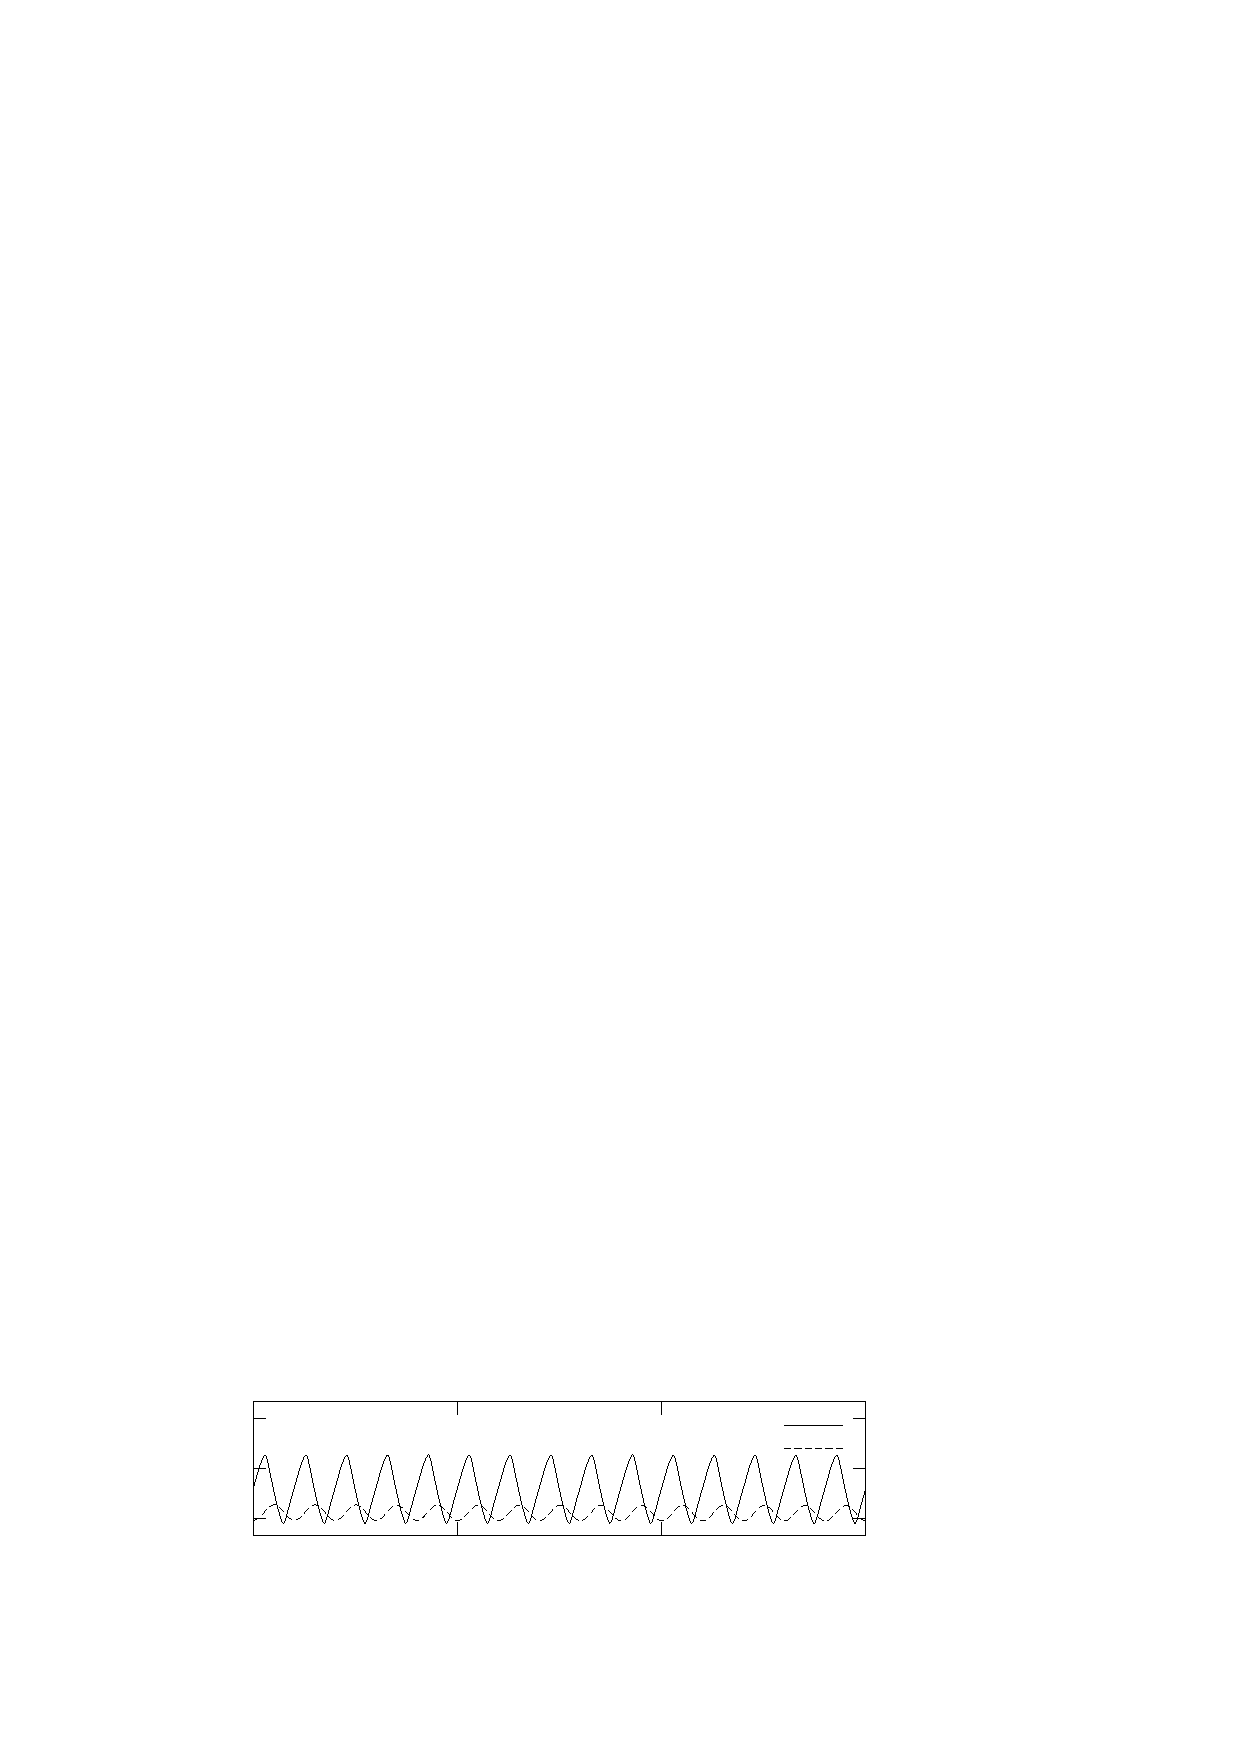
\includegraphics{detalle-rounded-flat-gravity}%
%\end{picture}%
%\begingroup
%\setlength{\unitlength}{0.0200bp}%
%\begin{picture}(18000,5400)(0,0)%
%\put(2200,2050){\makebox(0,0)[r]{\strut{}1.35}}%
%\put(2200,3250){\makebox(0,0)[r]{\strut{}1.50}}%
%\put(2200,4450){\makebox(0,0)[r]{\strut{}1.65}}%
%\put(2475,1100){\makebox(0,0){\strut{} 260}}%
%\put(7375,1100){\makebox(0,0){\strut{} 265}}%
%\put(12275,1100){\makebox(0,0){\strut{} 270}}%
%\put(17175,1100){\makebox(0,0){\strut{} 275}}%
%\put(550,3250){\rotatebox{90}{\makebox(0,0){\strut{}$y^\ast$}}}%
%\put(9825,275){\makebox(0,0){\strut{}$t^\ast$}}%
%\put(14950,4275){\makebox(0,0)[r]{\strut{}redondeada}}%
%\put(14950,3725){\makebox(0,0)[r]{\strut{}plana}}%
%%\put(600,1000){\rotatebox{0}{\makebox(0,0){\strut{}(a)}}}%
%\end{picture}%
%\endgroup
%\endinput

%GNUPLOT: LaTeX picture with Postscript
\begin{picture}(0,0)%
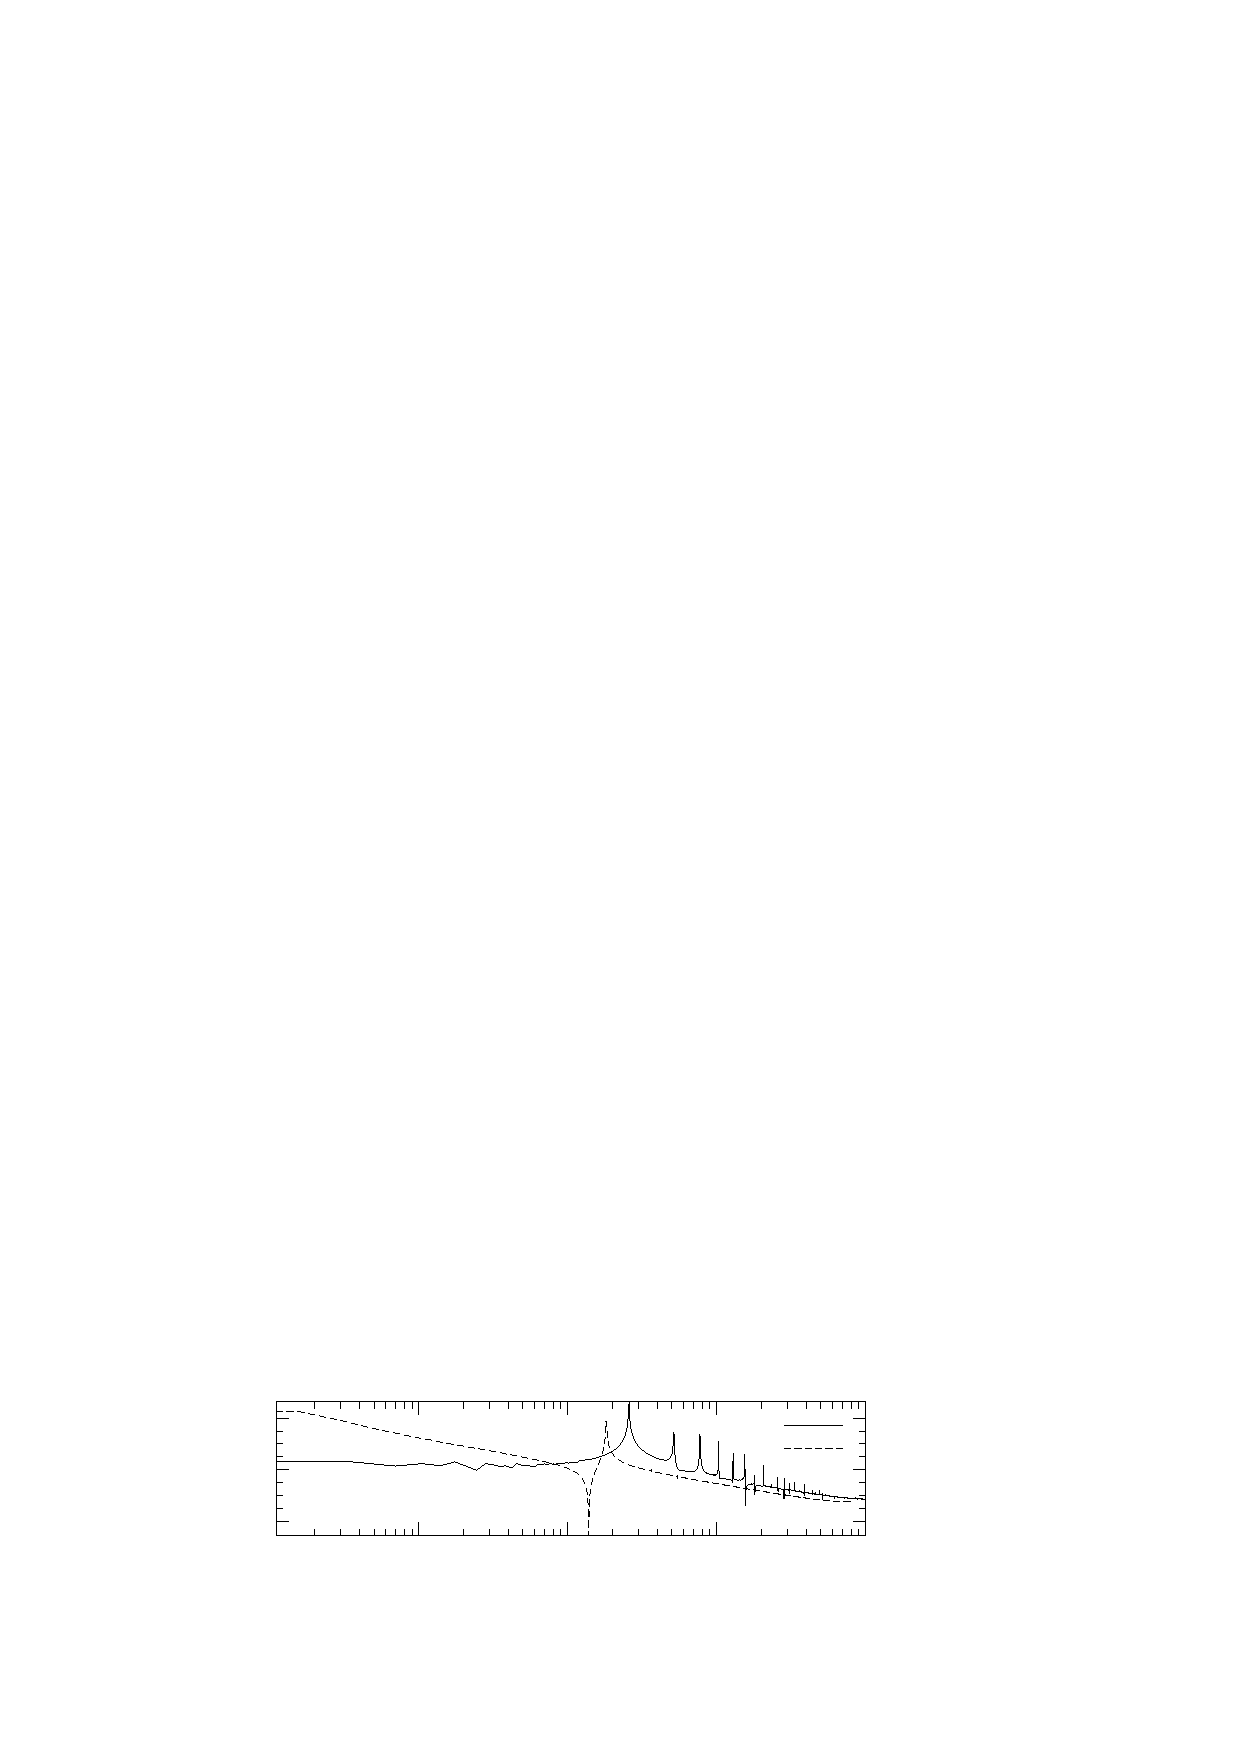
\includegraphics{detalle-frecuencias-rounded-flat-gravity}%
\end{picture}%
\begingroup
\setlength{\unitlength}{0.0200bp}%
\begin{picture}(18000,5400)(0,0)%
\put(2750,1989){\makebox(0,0)[r]{\strut{} 1e-12}}%
\put(2750,3223){\makebox(0,0)[r]{\strut{} 1e-08}}%
\put(2750,4458){\makebox(0,0)[r]{\strut{} 1e-04}}%
\put(6452,1100){\makebox(0,0){\strut{} 0.001}}%
\put(10026,1100){\makebox(0,0){\strut{} 0.01}}%
\put(13601,1100){\makebox(0,0){\strut{} 0.1}}%
\put(17175,1100){\makebox(0,0){\strut{} 1}}%
\put(550,3250){\rotatebox{90}{\makebox(0,0){\strut{}PSD}}}%
\put(10100,275){\makebox(0,0){\strut{}$\omega$}}%
\put(14950,4275){\makebox(0,0)[r]{\strut{}redondeada}}%
\put(14950,3725){\makebox(0,0)[r]{\strut{}plana}}%
\put(600,1000){\rotatebox{0}{\makebox(0,0){\strut{}(b)}}}%
\end{picture}%
\endgroup
\endinput

\caption{\label{fig:detalle-flat-rounded-gravity}
(a) Detalle del movimiento de la part'icula para la cavidad
plana y la redondeada ambas en presencia de un campo gravitacional externo, 
(b) an'alisis de Fourier de las trayectorias mostradas en (a) para conocer su frecuencia.
Ambas trayectorias oscilan con la frecuencia de la fuente ac'ustica $\omega_p=0.018138$
para la cavidad plana
y $\omega_r = 0.019126$ para la cavidad redondeada.
}
\end{figure}


En las siguientes simulaciones num'ericas, se conservaron todos los par'ametros pero se agreg'o
la presencia de un campo gravitacional externo.  La posici'on de equilibrio se desplaza al lugar donde
la sumatoria de fuerzas ac'usticas es igual al peso de la part'icula. En las figuras~\ref{fig:path-3} (a)
y (b)  se muestra la evoluci'on temporal de la posici'on vertical de una part'icula s'olida en presencia 
de un campo gravitacional externo para la cavidad plana y la redondeada, respectivamente. 
La l'inea s'olida indica la posici'on de los nodos de presi'on para ambas cavidades, la amplitud de las variaciones en la
velocidad y en la presi'on es el mismo de las figuras~\ref{fig:nodos-presion-velocidad} (a) y (b).  
Se puede observar que el desplazamiento de la posici'on de equilibrio es mucho m'as grande para la cavidad plana y 
apenas es notorio para la cavidad redondeada. 
De las figuras~\ref{fig:detalle-flat-rounded-gravity} (a) y (b) se puede observar el mismo comportamiento para la trayectoria
de la part'icula que cuando no existe un campo gravitacional externo 
(ver figuras~\ref{fig:detalle-flat-rounded} (a) y (b) ).






\begin{figure}
%\put(15400,4350){\makebox(0,0)[r]{\strut{}(b)}}%
%GNUPLOT: LaTeX picture with Postscript
\begin{picture}(0,0)%
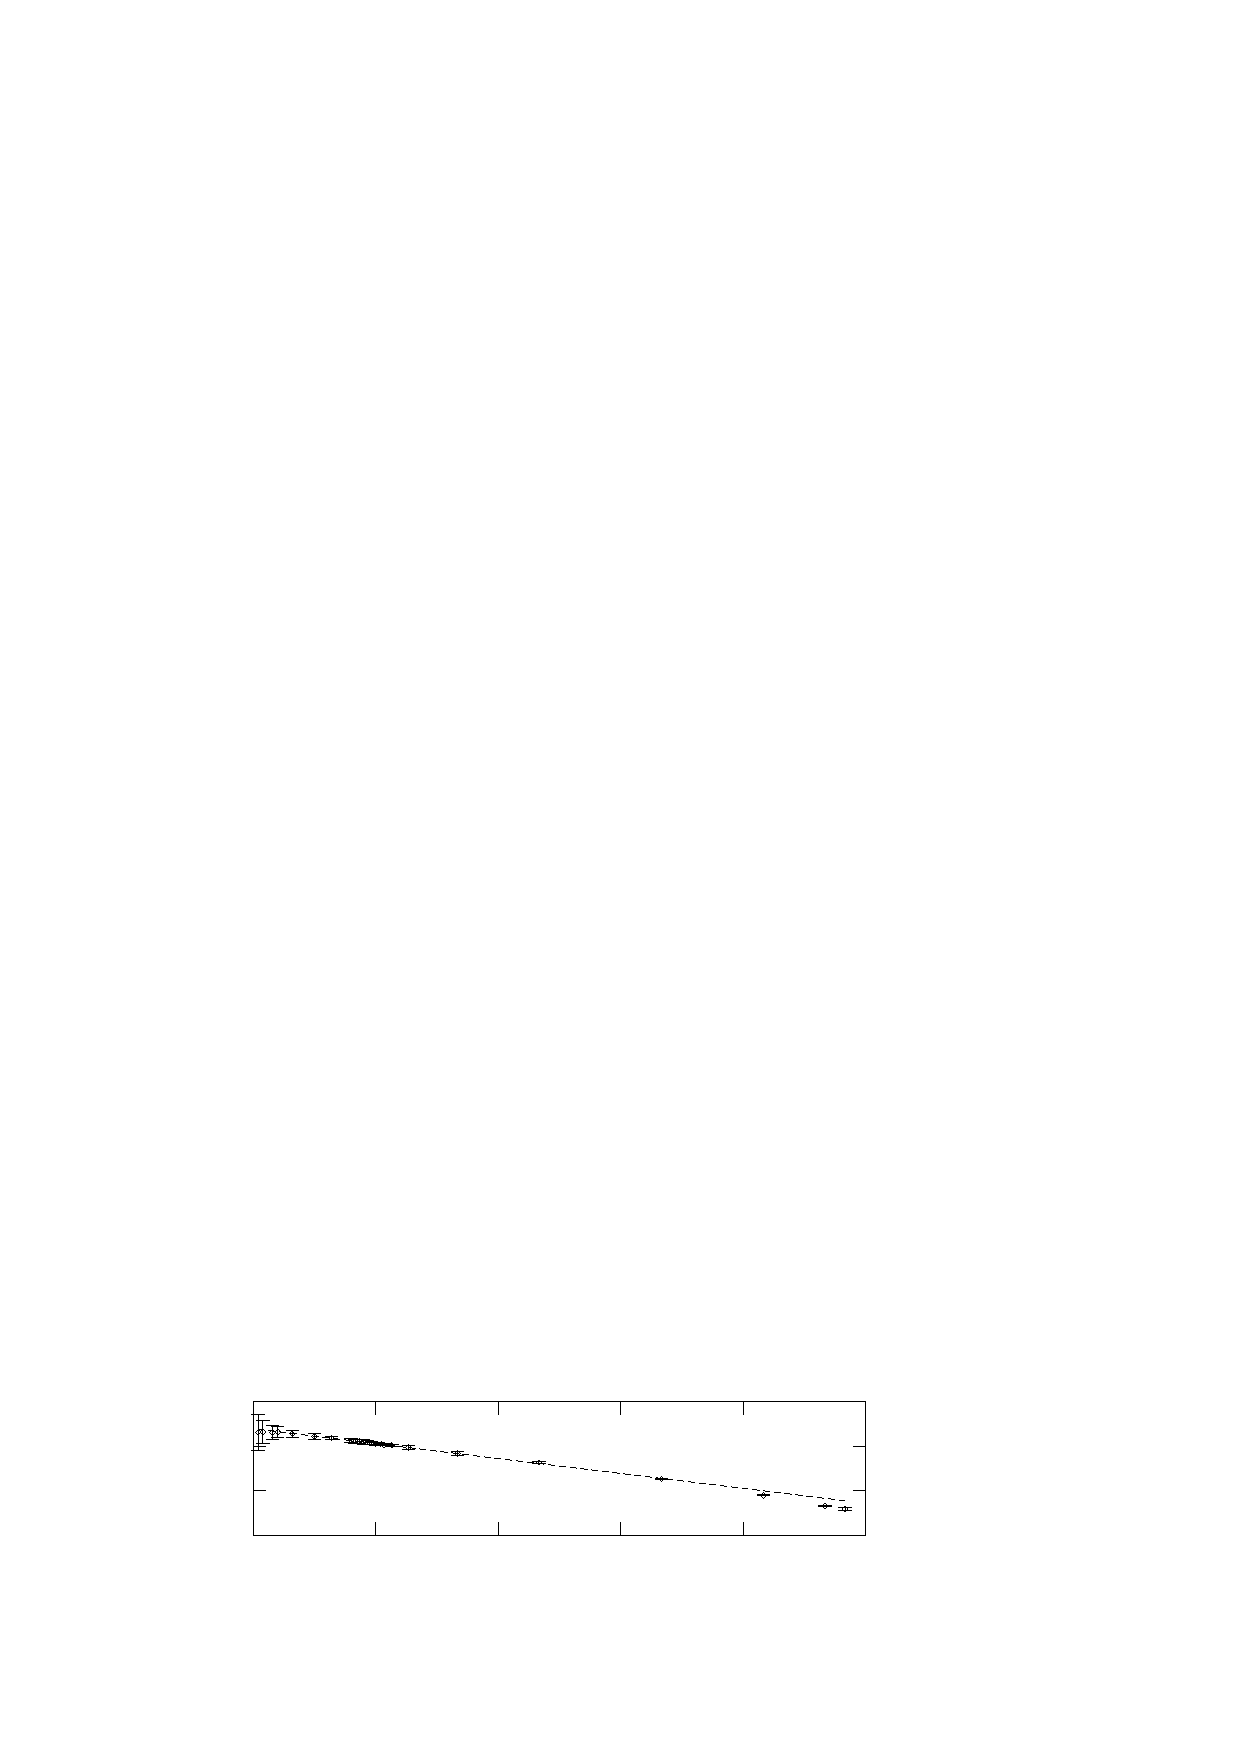
\includegraphics{barrido-rho-flat-ajuste}%
\end{picture}%
\begingroup
\setlength{\unitlength}{0.0200bp}%
\begin{picture}(18000,5400)(0,0)%
\put(2200,1650){\makebox(0,0)[r]{\strut{}1.00}}%
\put(2200,2717){\makebox(0,0)[r]{\strut{}1.25}}%
\put(2200,3783){\makebox(0,0)[r]{\strut{}1.50}}%
\put(2200,4850){\makebox(0,0)[r]{\strut{}1.75}}%
\put(2475,1100){\makebox(0,0){\strut{} 0}}%
\put(5415,1100){\makebox(0,0){\strut{} 50}}%
\put(8355,1100){\makebox(0,0){\strut{} 100}}%
\put(11295,1100){\makebox(0,0){\strut{} 150}}%
\put(14235,1100){\makebox(0,0){\strut{} 200}}%
\put(17175,1100){\makebox(0,0){\strut{} 250}}%
\put(550,3250){\rotatebox{90}{\makebox(0,0){\strut{}$y^\ast_{es}$}}}%
\put(9825,275){\makebox(0,0){\strut{}$\rho_p/\rho_f$}}%
\put(600,1000){\rotatebox{0}{\makebox(0,0){\strut{}(a)}}}%
\end{picture}%
\endgroup
\endinput

%GNUPLOT: LaTeX picture with Postscript
\begin{picture}(0,0)%
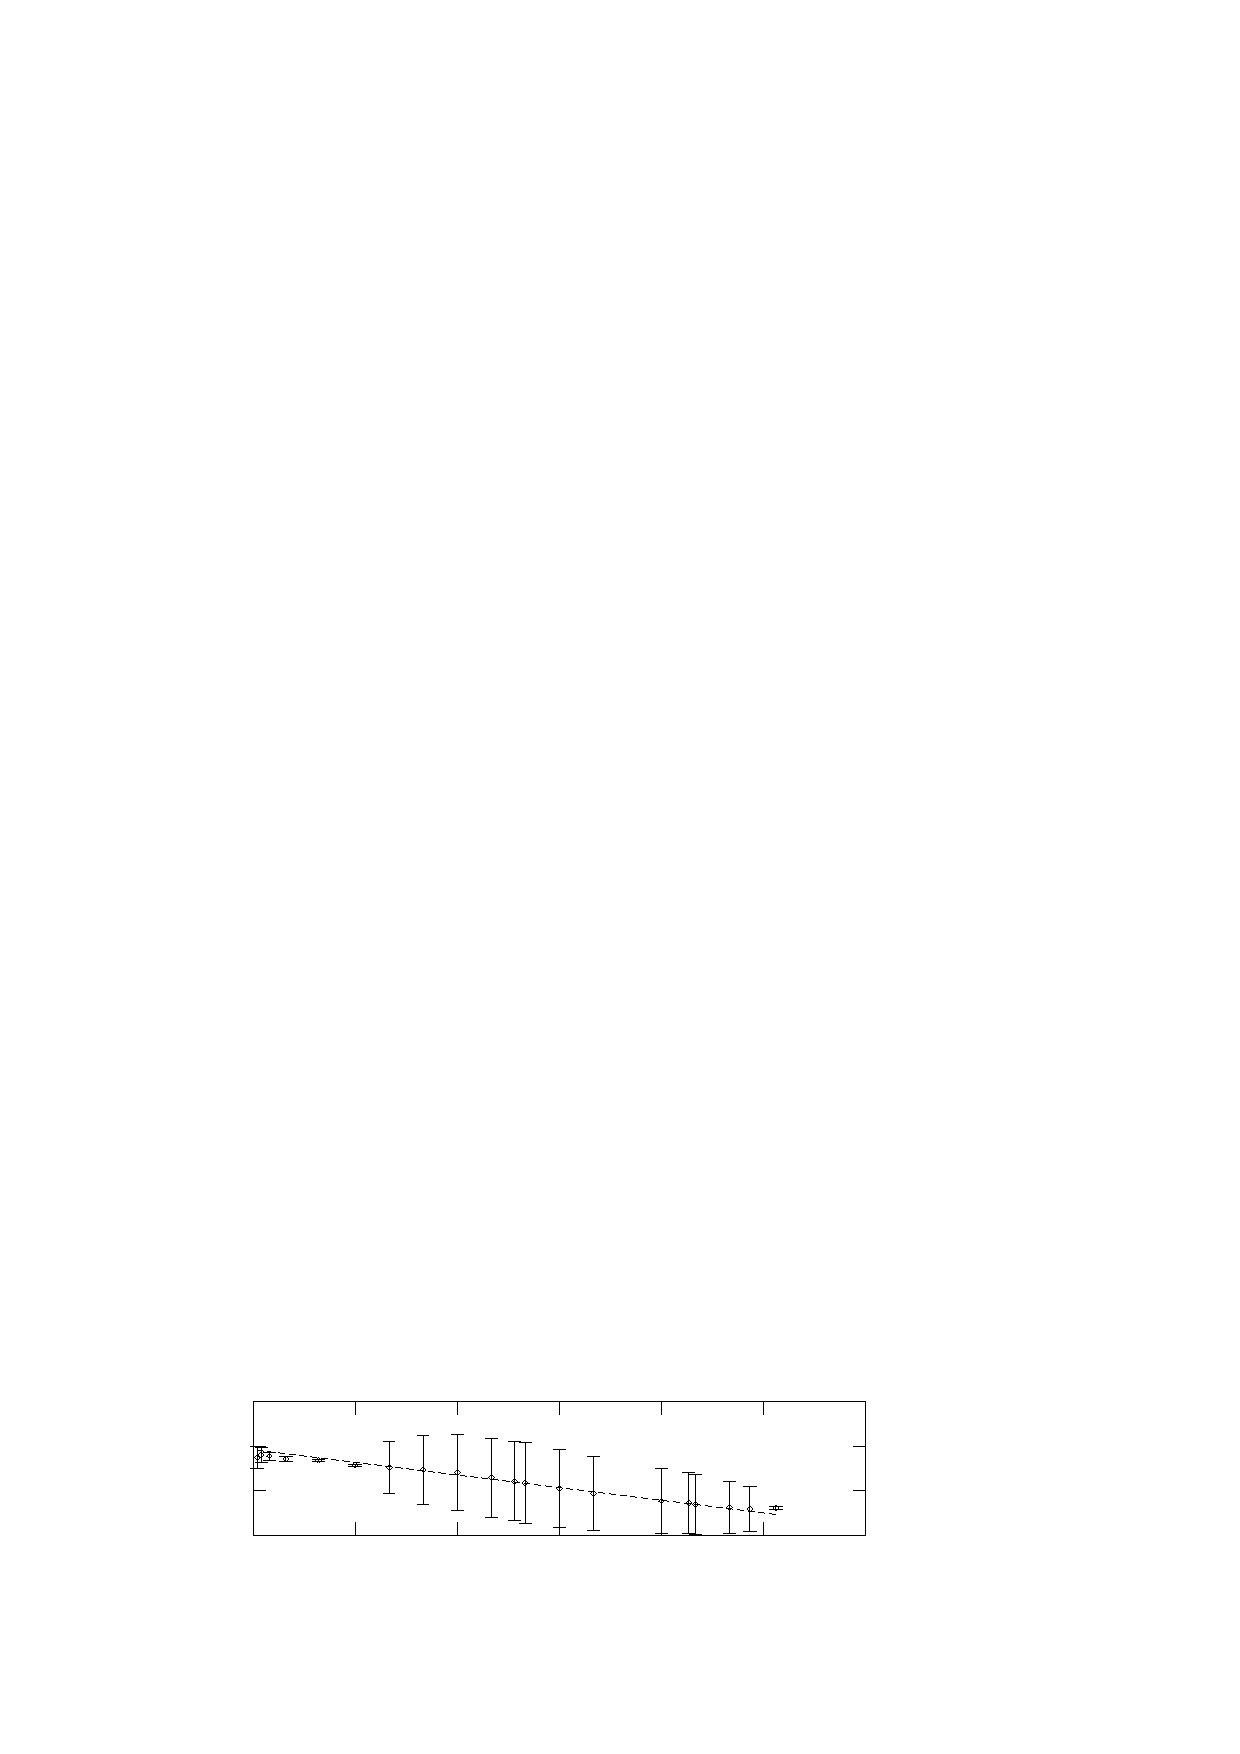
\includegraphics{barrido-rho-rounded-ajuste}%
\end{picture}%
\begingroup
\setlength{\unitlength}{0.0200bp}%
\begin{picture}(18000,5400)(0,0)%
\put(2200,1650){\makebox(0,0)[r]{\strut{}0.80}}%
\put(2200,2717){\makebox(0,0)[r]{\strut{}1.20}}%
\put(2200,3783){\makebox(0,0)[r]{\strut{}1.60}}%
\put(2200,4850){\makebox(0,0)[r]{\strut{}2.00}}%
\put(2475,1100){\makebox(0,0){\strut{} 0}}%
\put(4925,1100){\makebox(0,0){\strut{} 50}}%
\put(7375,1100){\makebox(0,0){\strut{} 100}}%
\put(9825,1100){\makebox(0,0){\strut{} 150}}%
\put(12275,1100){\makebox(0,0){\strut{} 200}}%
\put(14725,1100){\makebox(0,0){\strut{} 250}}%
\put(17175,1100){\makebox(0,0){\strut{} 300}}%
\put(550,3250){\rotatebox{90}{\makebox(0,0){\strut{}$y_{es}^\ast$}}}%
\put(9825,275){\makebox(0,0){\strut{}$\rho_p/\rho_f$}}%
\put(600,1000){\rotatebox{0}{\makebox(0,0){\strut{}(b)}}}%
\end{picture}%
\endgroup
\endinput

%GNUPLOT: LaTeX picture with Postscript
\begin{picture}(0,0)%
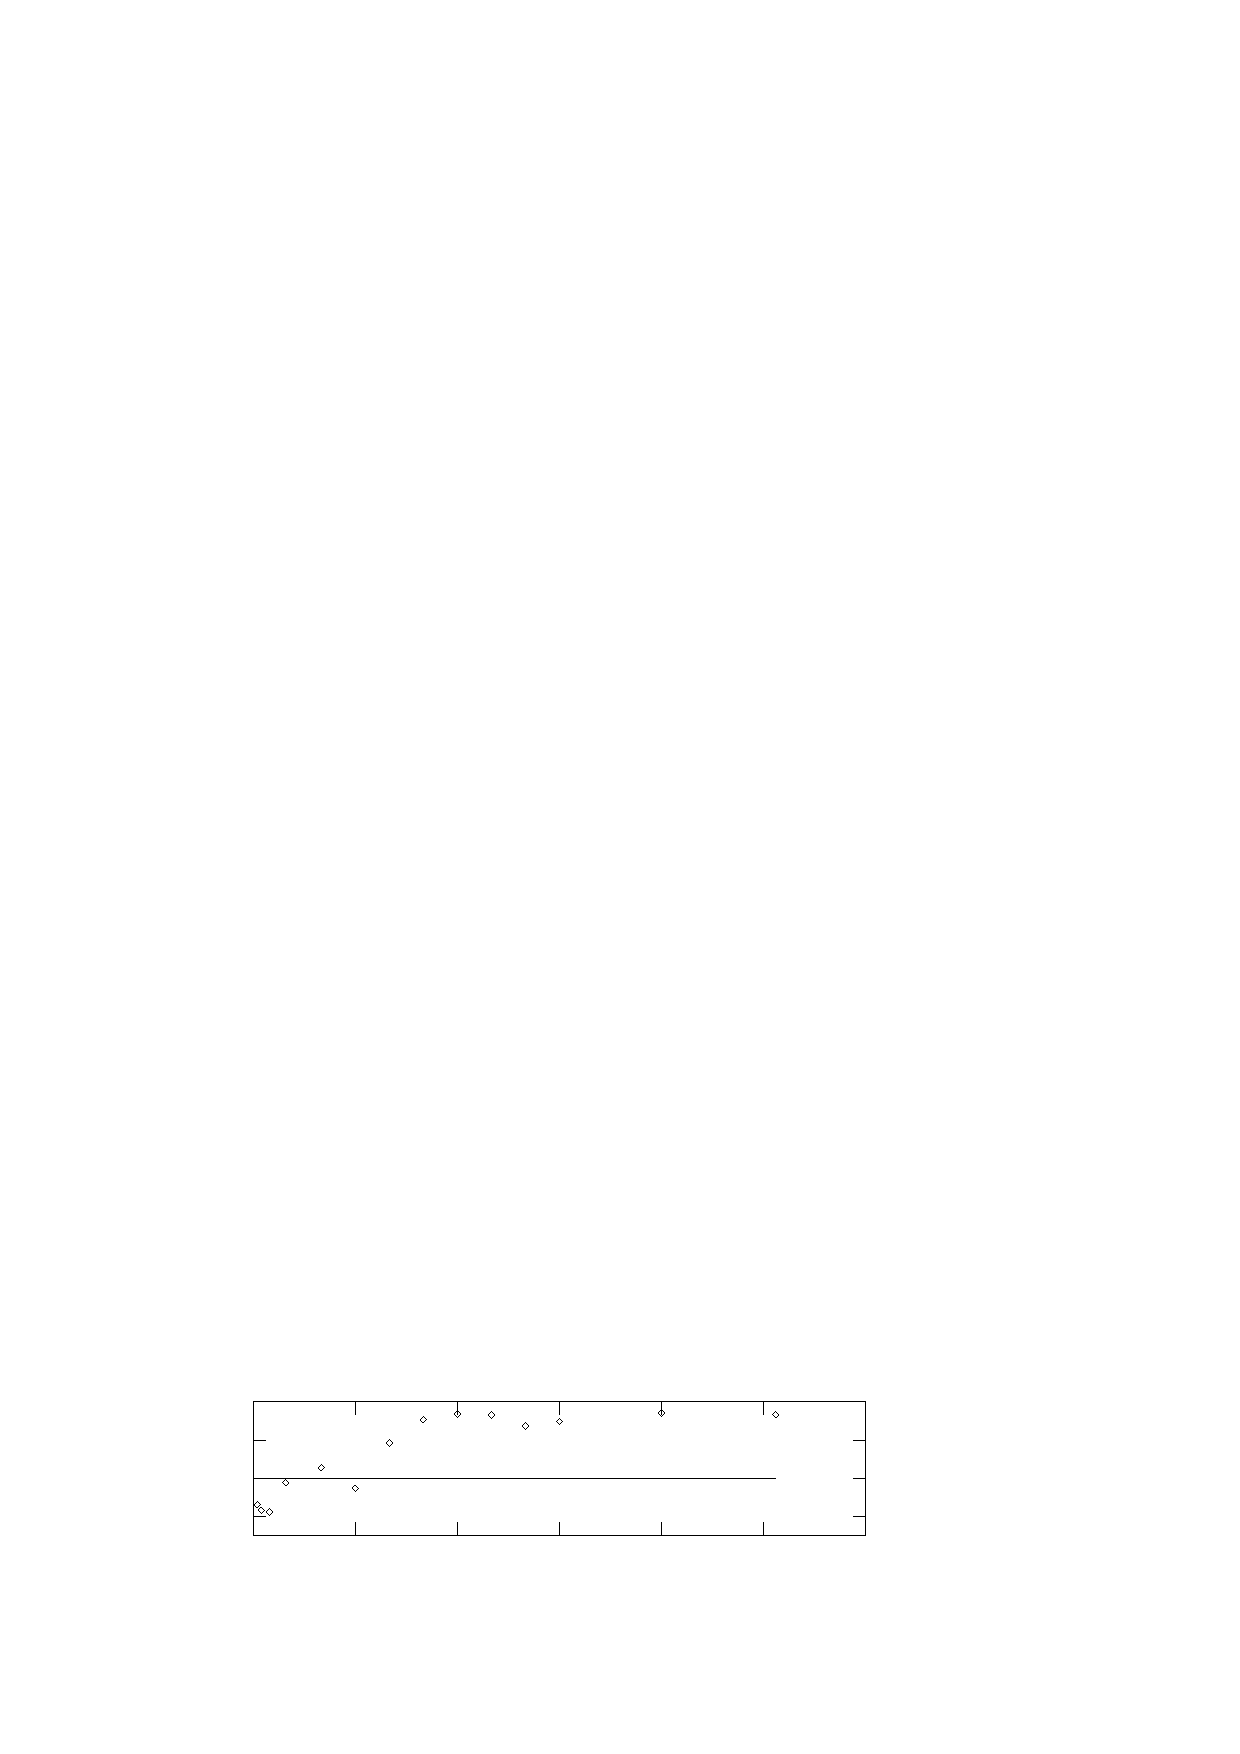
\includegraphics{resonancia-barridorho-rounded}%
\end{picture}%
\begingroup
\setlength{\unitlength}{0.0200bp}%
\begin{picture}(18000,5400)(0,0)%
\put(2200,2107){\makebox(0,0)[r]{\strut{}0.90}}%
\put(2200,3021){\makebox(0,0)[r]{\strut{}1.00}}%
\put(2200,3936){\makebox(0,0)[r]{\strut{}1.10}}%
\put(2200,4850){\makebox(0,0)[r]{\strut{}1.20}}%
\put(2475,1100){\makebox(0,0){\strut{} 0}}%
\put(4925,1100){\makebox(0,0){\strut{} 50}}%
\put(7375,1100){\makebox(0,0){\strut{} 100}}%
\put(9825,1100){\makebox(0,0){\strut{} 150}}%
\put(12275,1100){\makebox(0,0){\strut{} 200}}%
\put(14725,1100){\makebox(0,0){\strut{} 250}}%
\put(17175,1100){\makebox(0,0){\strut{} 300}}%
\put(550,3250){\rotatebox{90}{\makebox(0,0){\strut{}$v_{max}^\ast$}}}%
\put(9825,275){\makebox(0,0){\strut{}$\rho_p/\rho_f$}}%
\put(600,1000){\rotatebox{0}{\makebox(0,0){\strut{}(c)}}}%
\end{picture}%
\endgroup
\endinput

\caption{\label{fig:barrido-rho}
Los puntos con las barras de error representan la posici'on de equilibrio de la part'icula y
la desviaci'on est'andard $\sigma_y$, respectivamente. Se mantuvo fija la cantidad de movimiento
agregada en  (a) $P_o^\ast=0.01$ para la cavidad plana , (b) $P\ast=0.0019$ para la redondeada y 
se vari'o la relaci'on de densidad entre la part'icula y el fluido $\rho_p/\rho_f$ y (c) se midi'o
la velocidad m'axima dentro de la cavidad en presencia de part'icula  para la cavidad redondeada.
}
\end{figure}
%
\begin{figure}
%\put(-180,3250){\rotatebox{90}{\makebox(0,0){\strut{}(a)}}}%
%GNUPLOT: LaTeX picture with Postscript
%\begin{picture}(0,0)%
%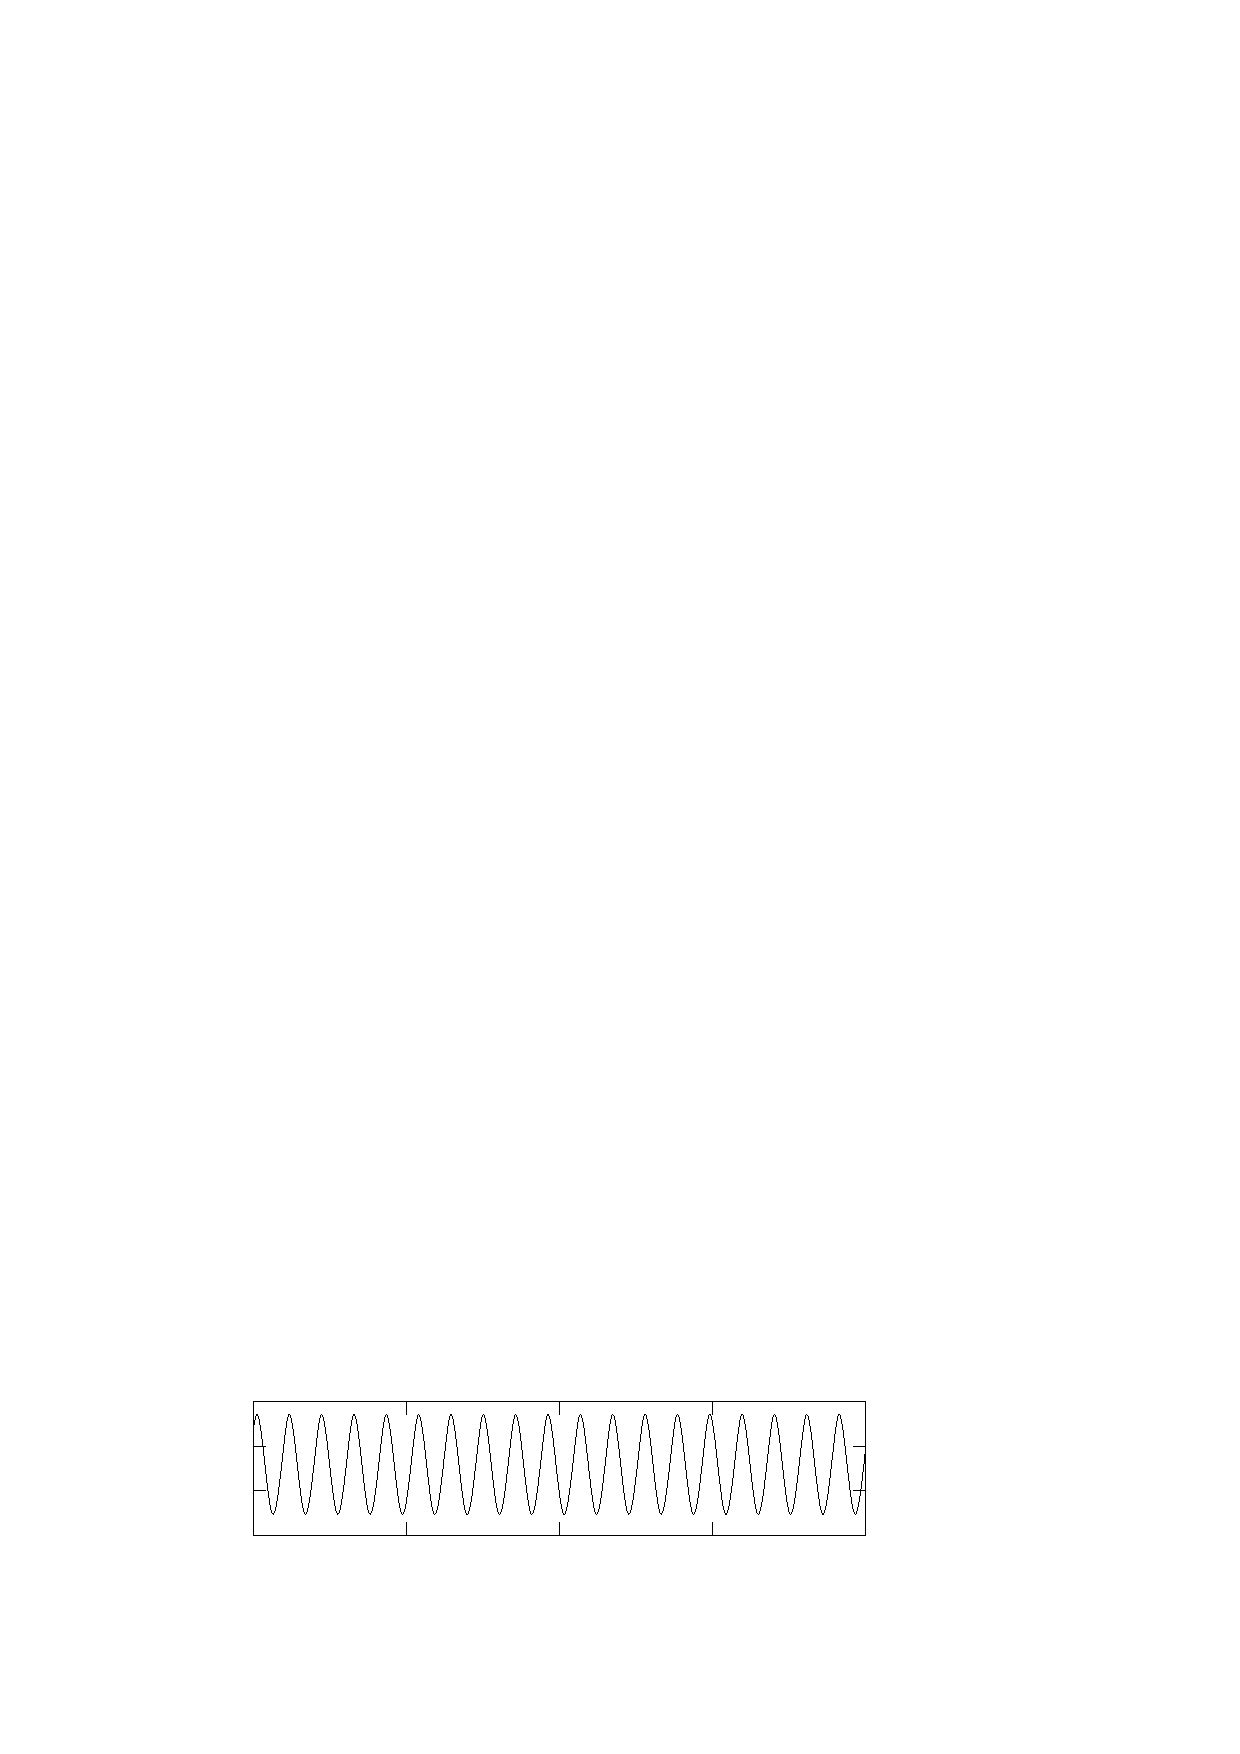
\includegraphics{flat-rhobarrido4_8}%
%\end{picture}%
%\begingroup
%\setlength{\unitlength}{0.0200bp}%
%\begin{picture}(18000,5400)(0,0)%
%\put(2200,1650){\makebox(0,0)[r]{\strut{}1.50}}%
%\put(2200,2717){\makebox(0,0)[r]{\strut{}1.55}}%
%\put(2200,3783){\makebox(0,0)[r]{\strut{}1.60}}%
%\put(2200,4850){\makebox(0,0)[r]{\strut{}1.65}}%
%\put(2475,1100){\makebox(0,0){\strut{} 500}}%
%\put(6150,1100){\makebox(0,0){\strut{} 505}}%
%\put(9825,1100){\makebox(0,0){\strut{} 510}}%
%\put(13500,1100){\makebox(0,0){\strut{} 515}}%
%\put(17175,1100){\makebox(0,0){\strut{} 520}}%
%\put(550,3250){\rotatebox{90}{\makebox(0,0){\strut{}$y^\ast$}}}%
%\put(9825,275){\makebox(0,0){\strut{}$t^\ast$}}%
%\put(600,1000){\rotatebox{0}{\makebox(0,0){\strut{}(a)}}}%
%\end{picture}%
%\endgroup
%\endinput

%GNUPLOT: LaTeX picture with Postscript
%\begin{picture}(0,0)%
%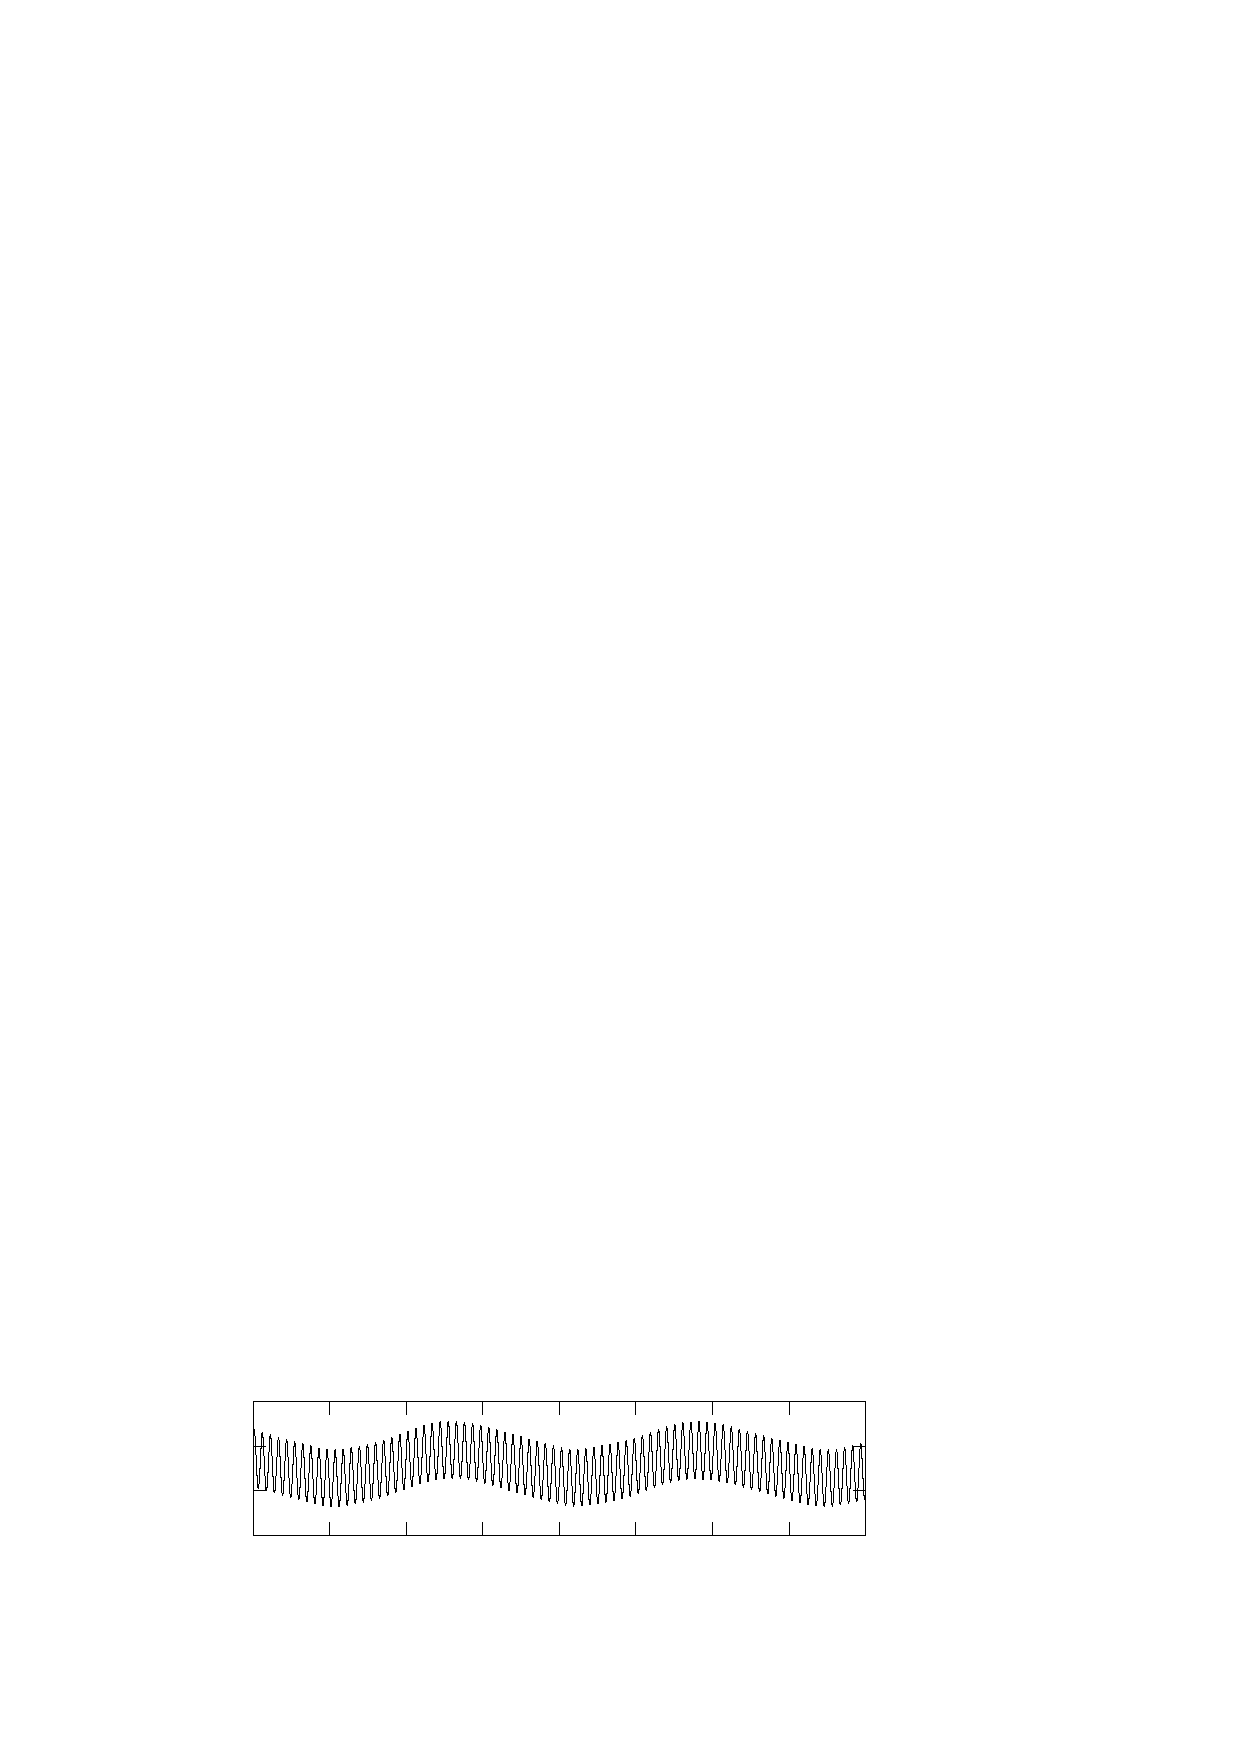
\includegraphics{flat-rhobarrido24}%
%\end{picture}%
%\begingroup
%\setlength{\unitlength}{0.0200bp}%
%\begin{picture}(18000,5400)(0,0)%
%\put(2200,1650){\makebox(0,0)[r]{\strut{}1.50}}%
%\put(2200,2717){\makebox(0,0)[r]{\strut{}1.52}}%
%\put(2200,3783){\makebox(0,0)[r]{\strut{}1.54}}%
%\put(2200,4850){\makebox(0,0)[r]{\strut{}1.56}}%
%\put(2475,1100){\makebox(0,0){\strut{} 500}}%
%\put(4313,1100){\makebox(0,0){\strut{} 510}}%
%\put(6150,1100){\makebox(0,0){\strut{} 520}}%
%\put(7988,1100){\makebox(0,0){\strut{} 530}}%
%\put(9825,1100){\makebox(0,0){\strut{} 540}}%
%\put(11663,1100){\makebox(0,0){\strut{} 550}}%
%\put(13500,1100){\makebox(0,0){\strut{} 560}}%
%\put(15338,1100){\makebox(0,0){\strut{} 570}}%
%\put(17175,1100){\makebox(0,0){\strut{} 580}}%
%\put(550,3250){\rotatebox{90}{\makebox(0,0){\strut{}$y^\ast$}}}%
%\put(9825,275){\makebox(0,0){\strut{}$t^\ast$}}%
%\put(600,1000){\rotatebox{0}{\makebox(0,0){\strut{}(b)}}}%
%\end{picture}%
%\endgroup
%\endinput

%GNUPLOT: LaTeX picture with Postscript
%\begin{picture}(0,0)%
%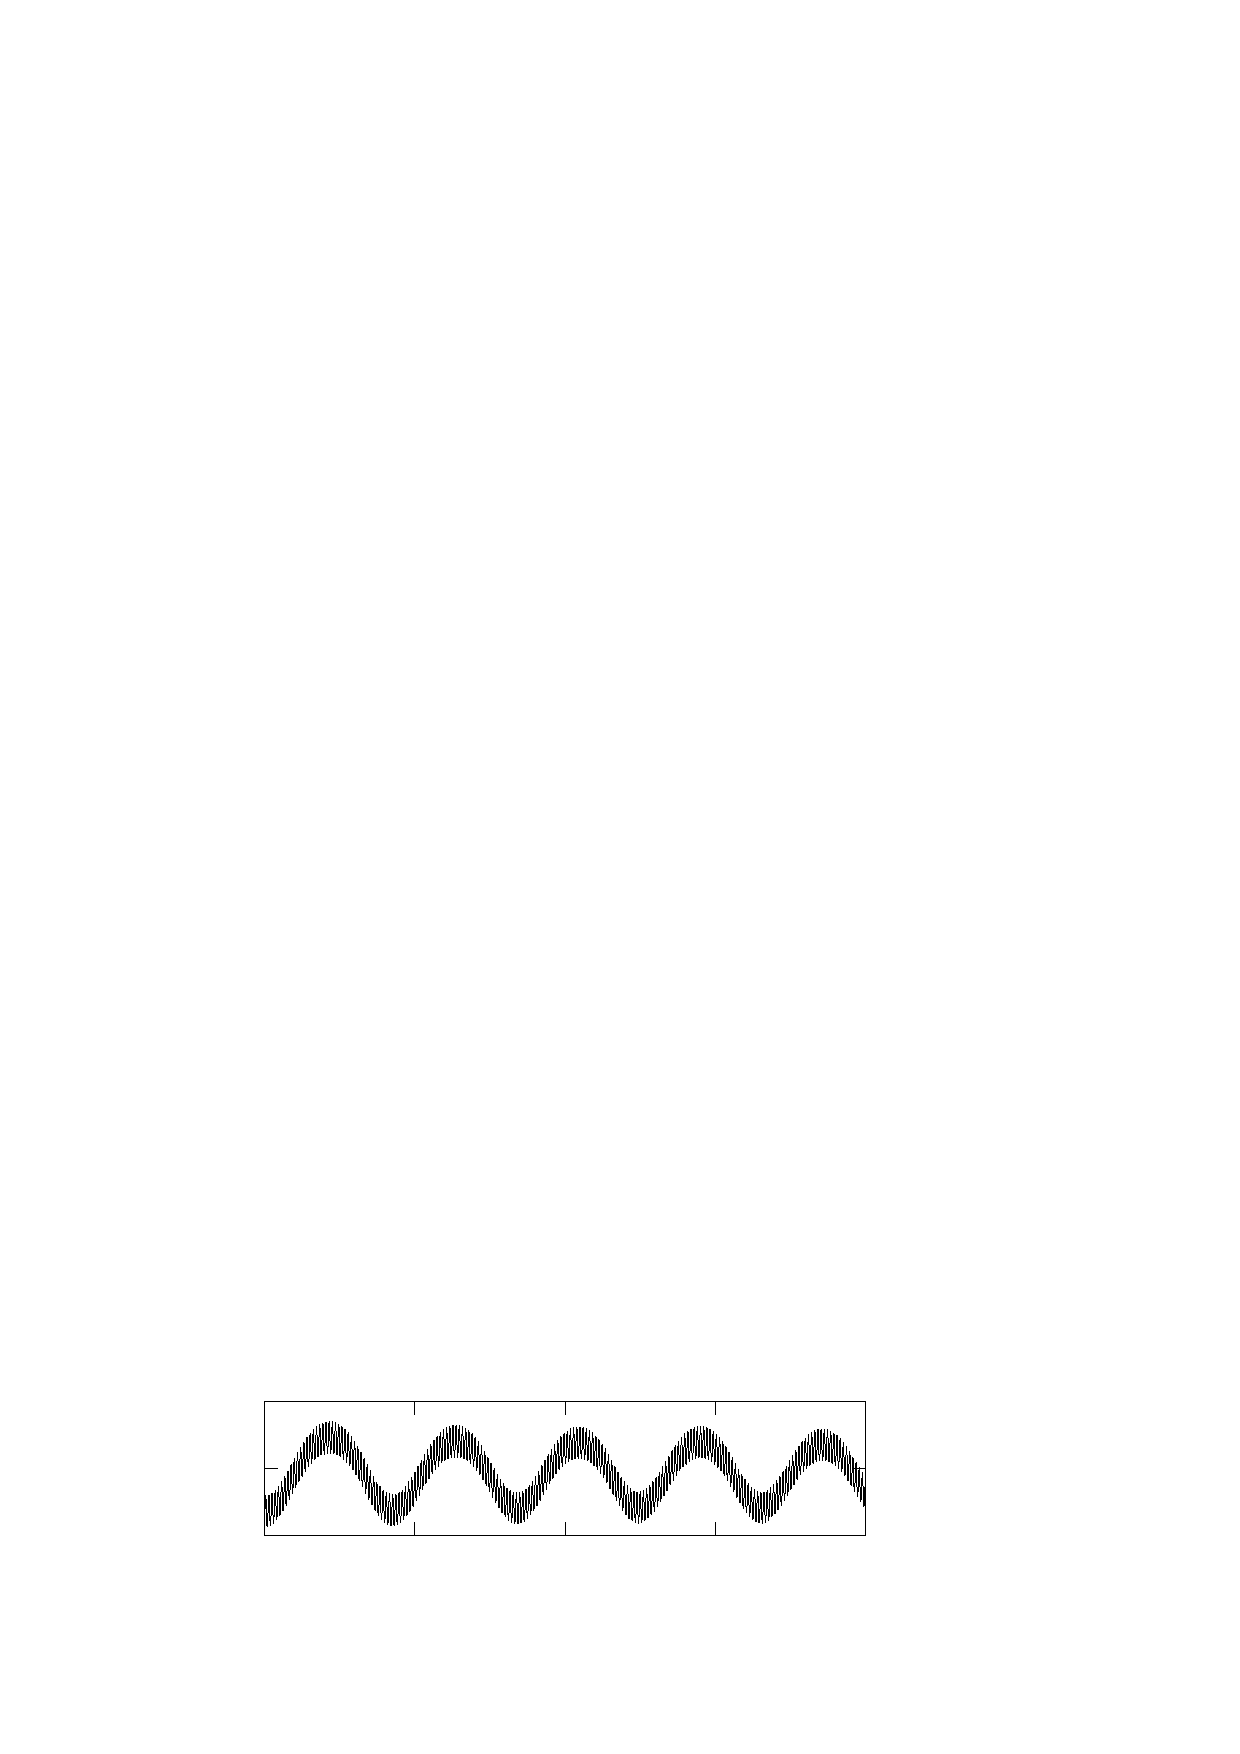
\includegraphics{flat-rhobarrido140}%
%\end{picture}%
%\begingroup
%\setlength{\unitlength}{0.0200bp}%
%\begin{picture}(18000,5400)(0,0)%
%\put(2475,1650){\makebox(0,0)[r]{\strut{}1.156}}%
%\put(2475,3250){\makebox(0,0)[r]{\strut{}1.165}}%
%\put(2475,4850){\makebox(0,0)[r]{\strut{}1.173}}%
%\put(2750,1100){\makebox(0,0){\strut{} 2950}}%
%\put(6356,1100){\makebox(0,0){\strut{} 3000}}%
%\put(9963,1100){\makebox(0,0){\strut{} 3050}}%
%\put(13569,1100){\makebox(0,0){\strut{} 3100}}%
%\put(17175,1100){\makebox(0,0){\strut{} 3150}}%
%\put(550,3250){\rotatebox{90}{\makebox(0,0){\strut{}$y^\ast$}}}%
%\put(9962,275){\makebox(0,0){\strut{}$t^\ast$}}%
%\put(600,1000){\rotatebox{0}{\makebox(0,0){\strut{}(c)}}}%
%\end{picture}%
%\endgroup
%\endinput

\caption{\label{fig:paths-flat}
Trayectoria de la posici'on vertical de la part'icula s'olida sobre el tiempo en la cavidad plana para
(a) $\rho_p/\rho_f = 8$, (b) $\rho_p/\rho_f = 40$ y (c) $\rho_p/\rho_f = 233.3$.}
\end{figure}
%
\begin{figure}
%\put(600,2550){\rotatebox{90}{\makebox(0,0){\strut{}(a)}}}%
%GNUPLOT: LaTeX picture with Postscript
%\begin{picture}(0,0)%
%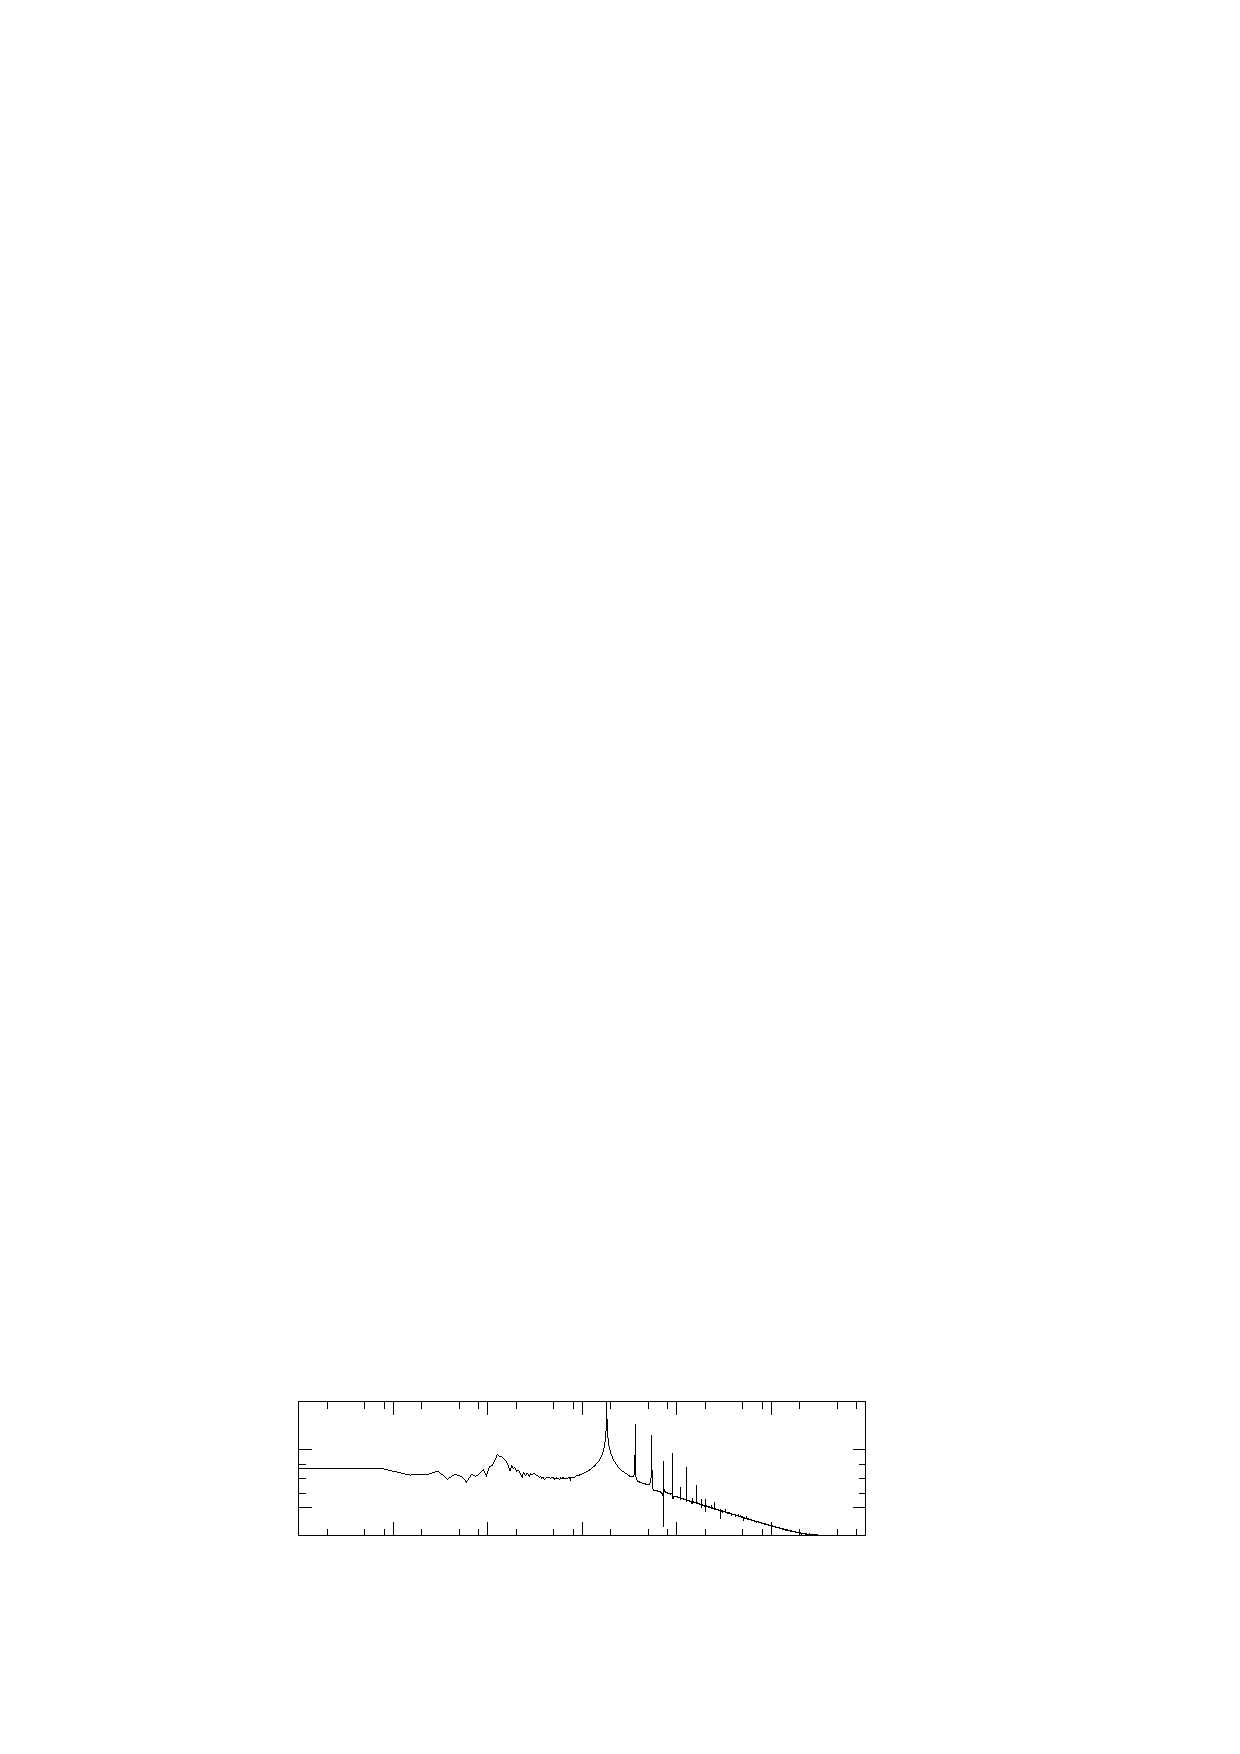
\includegraphics{flat-rhobarrido4_8-spectrum}%
%\end{picture}%
%\begingroup
%\setlength{\unitlength}{0.0200bp}%
%\begin{picture}(18000,5400)(0,0)%
%\put(3300,2307){\makebox(0,0)[r]{\strut{}1.00e-12}}%
%\put(3300,3707){\makebox(0,0)[r]{\strut{}1.00e-08}}%
%\put(3575,1100){\makebox(0,0){\strut{} 1e-05}}%
%\put(5842,1100){\makebox(0,0){\strut{} 1e-04}}%
%\put(8108,1100){\makebox(0,0){\strut{} 0.001}}%
%\put(10375,1100){\makebox(0,0){\strut{} 0.01}}%
%\put(12642,1100){\makebox(0,0){\strut{} 0.1}}%
%\put(14908,1100){\makebox(0,0){\strut{} 1}}%
%\put(17175,1100){\makebox(0,0){\strut{} 10}}%
%\put(550,3250){\rotatebox{90}{\makebox(0,0){\strut{}$PSD$}}}%
%\put(10375,275){\makebox(0,0){\strut{}$\omega$}}%
%\put(600,1000){\rotatebox{0}{\makebox(0,0){\strut{}(a)}}}%
%\end{picture}%
%\endgroup
%\endinput

%GNUPLOT: LaTeX picture with Postscript
%\begin{picture}(0,0)%
%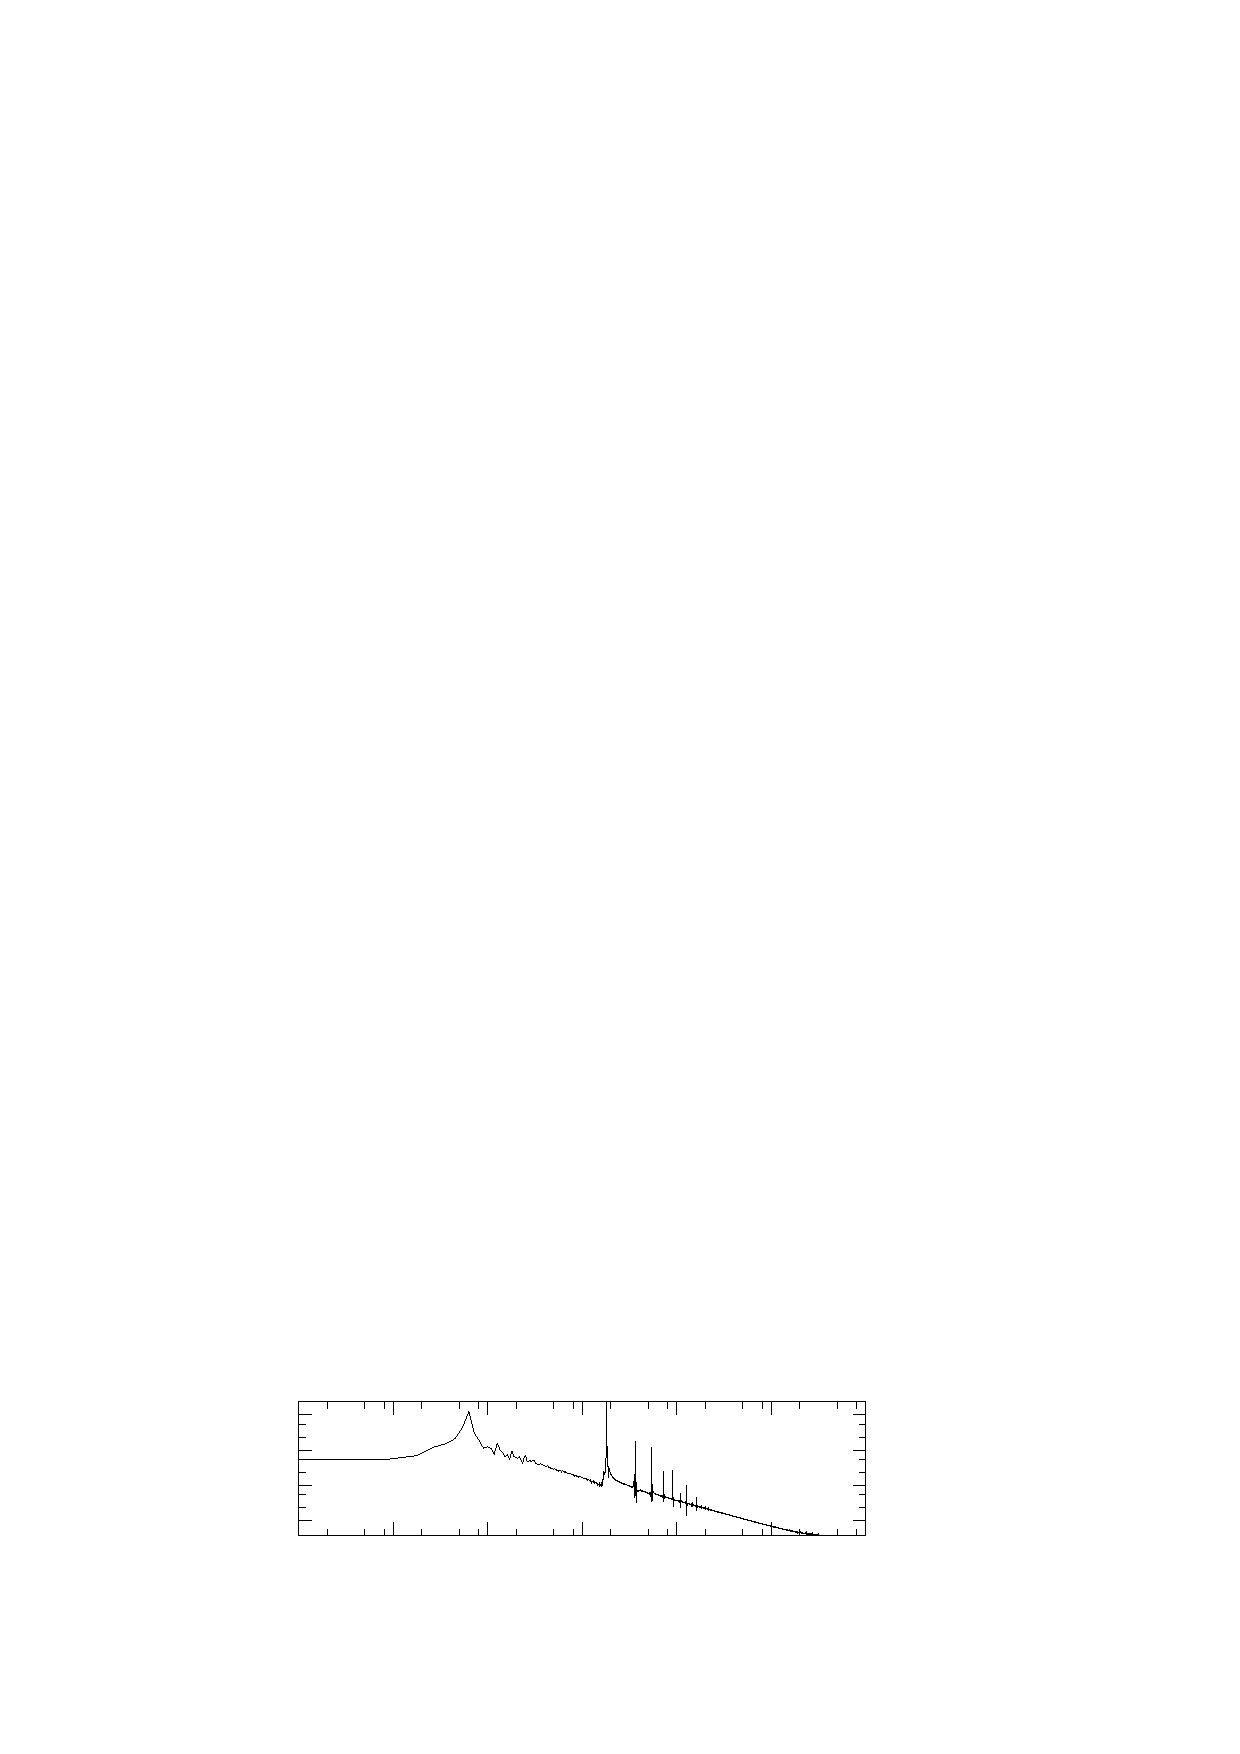
\includegraphics{flat-rhobarrido24-spectrum}%
%\end{picture}%
%\begingroup
%\setlength{\unitlength}{0.0200bp}%
%\begin{picture}(18000,5400)(0,0)%
%\put(3300,2000){\makebox(0,0)[r]{\strut{}3.20e-14}}%
%\put(3300,2846){\makebox(0,0)[r]{\strut{}1.60e-11}}%
%\put(3300,3693){\makebox(0,0)[r]{\strut{}8.00e-09}}%
%\put(3300,4539){\makebox(0,0)[r]{\strut{}4.00e-06}}%
%\put(3575,1100){\makebox(0,0){\strut{} 1e-05}}%
%\put(5842,1100){\makebox(0,0){\strut{} 1e-04}}%
%\put(8108,1100){\makebox(0,0){\strut{} 0.001}}%
%\put(10375,1100){\makebox(0,0){\strut{} 0.01}}%
%\put(12642,1100){\makebox(0,0){\strut{} 0.1}}%
%\put(14908,1100){\makebox(0,0){\strut{} 1}}%
%\put(17175,1100){\makebox(0,0){\strut{} 10}}%
%\put(550,3250){\rotatebox{90}{\makebox(0,0){\strut{}$PSD$}}}%
%\put(10375,275){\makebox(0,0){\strut{}$\omega$}}%
%\put(600,1000){\rotatebox{0}{\makebox(0,0){\strut{}(b)}}}%
%\end{picture}%
%\endgroup
%\endinput

%GNUPLOT: LaTeX picture with Postscript
%\begin{picture}(0,0)%
%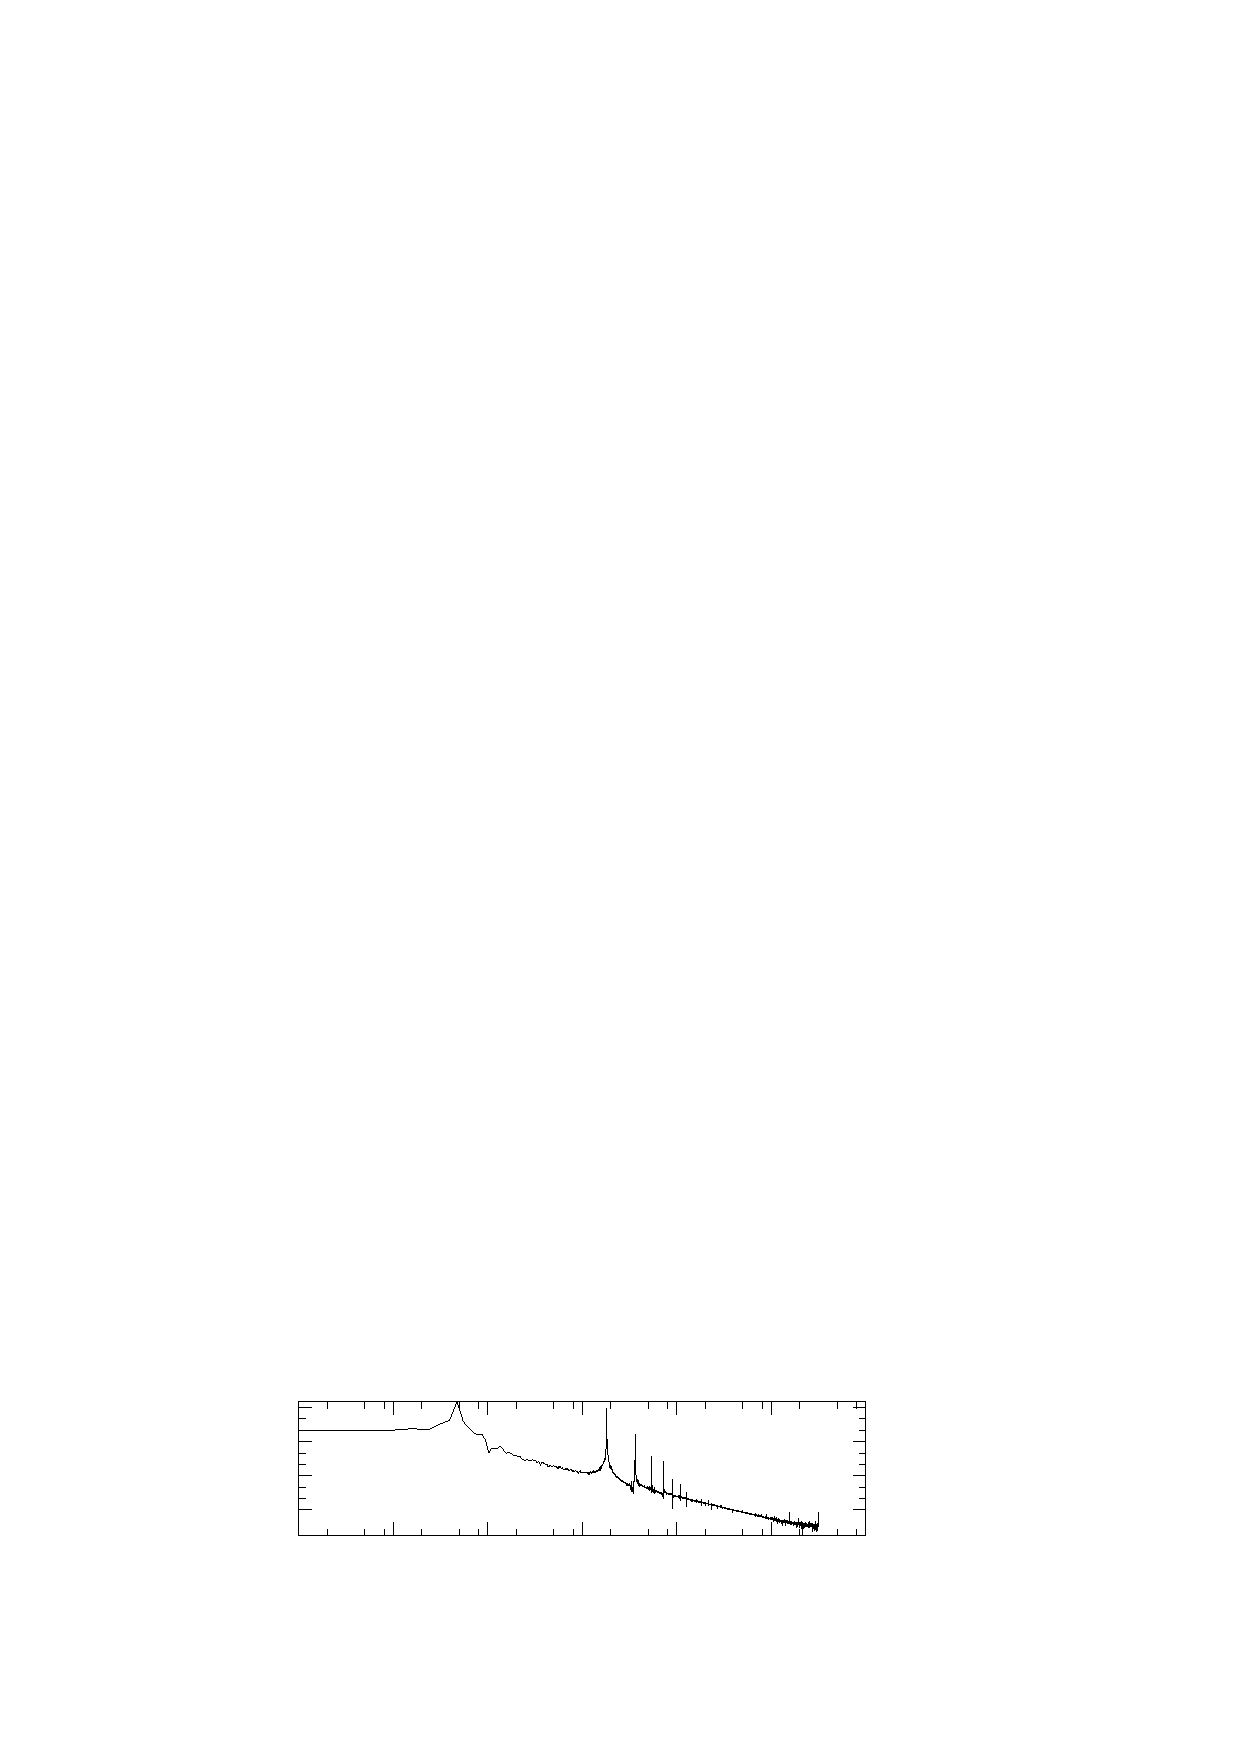
\includegraphics{flat-rhobarrido140-spectrum}%
%\end{picture}%
%\begingroup
%\setlength{\unitlength}{0.0200bp}%
%\begin{picture}(18000,5400)(0,0)%
%\put(3300,2259){\makebox(0,0)[r]{\strut{}1.00e-15}}%
%\put(3300,3077){\makebox(0,0)[r]{\strut{}1.00e-12}}%
%\put(3300,3896){\makebox(0,0)[r]{\strut{}1.00e-09}}%
%\put(3300,4714){\makebox(0,0)[r]{\strut{}1.00e-06}}%
%\put(3575,1100){\makebox(0,0){\strut{} 1e-05}}%
%\put(5842,1100){\makebox(0,0){\strut{} 1e-04}}%
%\put(8108,1100){\makebox(0,0){\strut{} 0.001}}%
%\put(10375,1100){\makebox(0,0){\strut{} 0.01}}%
%\put(12642,1100){\makebox(0,0){\strut{} 0.1}}%
%\put(14908,1100){\makebox(0,0){\strut{} 1}}%
%\put(17175,1100){\makebox(0,0){\strut{} 10}}%
%\put(550,3250){\rotatebox{90}{\makebox(0,0){\strut{}$PSD$}}}%
%\put(10375,275){\makebox(0,0){\strut{}$\omega$}}%
%\put(600,1000){\rotatebox{0}{\makebox(0,0){\strut{}(c)}}}%
%\end{picture}%
%\endgroup
%\endinput

\caption{\label{fig:spectrum-flat}
Espectros de potencia del movimiento vertical de la part'icula s'olida sobre el tiempo en la cavidad plana para
(a) $\rho_p/\rho_f = 8$, (b) $\rho_p/\rho_f = 40$ y (c) $\rho_p/\rho_f = 233.3$. 
Los espectros de potencia corresponden a los de las figuras~\ref{fig:paths-flat} (a), (b) y (c). }
\end{figure}


En el siguiente conjunto de simulaciones num'ericas se mantuvo constante
la cantidad de movimiento agregada a la fuente ac'ustica $P_o^\ast$ y se 
vari'o la relaci'on de densidades entre la part'icula y el fluido $\rho_p/\rho_f$. Para
la cavidad plana se fij'o la cantidad de movimiento 
en $P_o^\ast=0.01$ y para la cavidad redondeada en $P_o^\ast=0.0019$.
El movimiento de la part'icula, como se mostrar'a m'as adelante, puede llegar a ser 
muy complejo, por lo que adem'as de la posici'on de equilibrio, se mide la desviaci'on est'andard 
del movimiento de la part'icula en ambos ejes $(\sigma_x,\sigma_y)$  para ambas cavidades, 
como se puede ver en las figuras~\ref{fig:barrido-rho} (a) y (b), donde el punto
representa a la posici'on de equilibrio y la barra de error $\sigma_y$. El valor de
$\sigma_x=0$ a menos que se diga lo contrario.  Para la cavidad plana, el valor
m'as grande de $\sigma_y$ se presenta para $\rho_p/\rho_f=2$. Conforme
la relaci'on de densidades aumenta, es m'as dificil que el campo ac'ustico pueda mover la part'icula
y  la posici'on de equilibrio se desplaza hacia abajo, como se
puede observar en la figura~\ref{fig:barrido-rho} (a). El valor m'aximo de la desviaci'on
est'andar en el eje vertical es $\sigma_y^\ast = 0.1$ para $\rho_p/\rho_f = 2$ y el m'inimo
es $\sigma_y^\ast = 0.002$ para $\rho_p/\rho_f = 166.6$. El desplazamiento de la posici'on
de equilibrio se mueve en l'inea recta entre $40< \rho_p/\rho_f < 200$, como se puede
observar del ajuste en la figura~\ref{fig:barrido-rho} (a).
Para la cavidad redondeada
el comportamiento resulta similar hasta $\rho_p/\rho_f=50$, la amplitud de oscilaci'on
decrece y la posici'on de equilibrio se desplaza hacia abajo, pero para $\rho_p/\rho_f > 50$
la amplitud de la oscilaci'on aumenta para luego disminuir nuevamente. Cuando se calcul'o
la resonancia de la cavidad redondeada se hizo en ausencia de la part'icula. Se sabe
que existe un desplazamiento en la frecuencia de resonancia y que es funci'on del tama~no 
y posici'on de la part'icula~\cite{leung82}. 
Para verificar lo anterior, se midi'o la velocidad m'axima del fluido dentro de la cavidad
redondeada en presencia de la part'icula, mostrada en la figura~\ref{fig:barrido-rho} (c). La velocidad
se escal'o con la velocidad m'axima del conjunto de simulaciones num'ericas. Como se puede
observar,  hay un aumento en la magnitud de la velocidad m'axima, sobre todo en la zona donde
la oscilaci'on de la part'icula crece, lo que indica un posible desplazamiento
de la frecuencia de resonancia debido a la presencia de la part'icula.
En la cavidad redondeada, el desplazamiento de la posici'on de equilibrio tambi'en sigue una 
l'inea recta en una zona, entre $50<\rho_p/\rho_f < 230$, como se puede observar
en la figura~\ref{fig:barrido-rho} (b) por el ajuste de la l'inea discontinua.






El movimiento de la part'icula puede presentar diversos comportamientos, como veremos
a continuaci'on. En la cavidad plana, a'un cuando la figura~\ref{fig:barrido-rho} (a) pudiera
sugerir un comportamiento mon'otono, no es as'i. Como se ve en las figuras~\ref{fig:paths-flat} (a),
(b) y (c) para  $\rho_p/\rho_f = 8$,  $\rho_p/\rho_f = 40$ y  $\rho_p/\rho_f = 233.3$, 
respectivamente., este movimiento se puede clasificar en dos tipos. 
En el primero, mostrado en la figura~\ref{fig:paths-flat} (a), la part'icula oscila alrededor de la posici'on de equilibrio
con amplitud $\sigma_y = 0.04$ y frecuencia $\omega_p=0.018138$. En el segundo comportamiento,  mostrado en la
figura~\ref{fig:paths-flat} (b), aparece una segunda frecuencia de oscilaci'on mucho menor que 
la frecuencia de oscilaci'on de la fuente ac'ustica y la oscilaci'on de la part'icula es 
$\sigma_y = 0.009$. En la figura~\ref{fig:paths-flat} (c) se muestra el movimiento de la part'icula 
para $\rho_p/\rho_f = 233.3$, que es muy similar al mostrado para  $\rho_p/\rho_f = 40$ con
$\sigma_y = 0.0035$.  
En las figuras~\ref{fig:spectrum-flat} (a), (b) y (c) se muestra el an'alisis de Fourier 
del movimiento de la part'icula, y se confirma que para   $\rho_p/\rho_f = 8$ 
el movimiento de la part'icula est'a dado por la frecuencia de la fuente ac'ustica y sus arm'onicos, 
y para   $\rho_p/\rho_f = 40$ y  $\rho_p/\rho_f = 233.3$ aparece una segunda frecuencia de oscilaci'on 
tres ordenes de magnitud m'as baja. En todos los casos existen los arm'onicos de la frecuencia de
la fuente ac'ustica en el movimiento de la part'icula.




	
\begin{figure}
%\put(600,2550){\rotatebox{90}{\makebox(0,0){\strut{}(a)}}}%
%GNUPLOT: LaTeX picture with Postscript
%\begin{picture}(0,0)%
%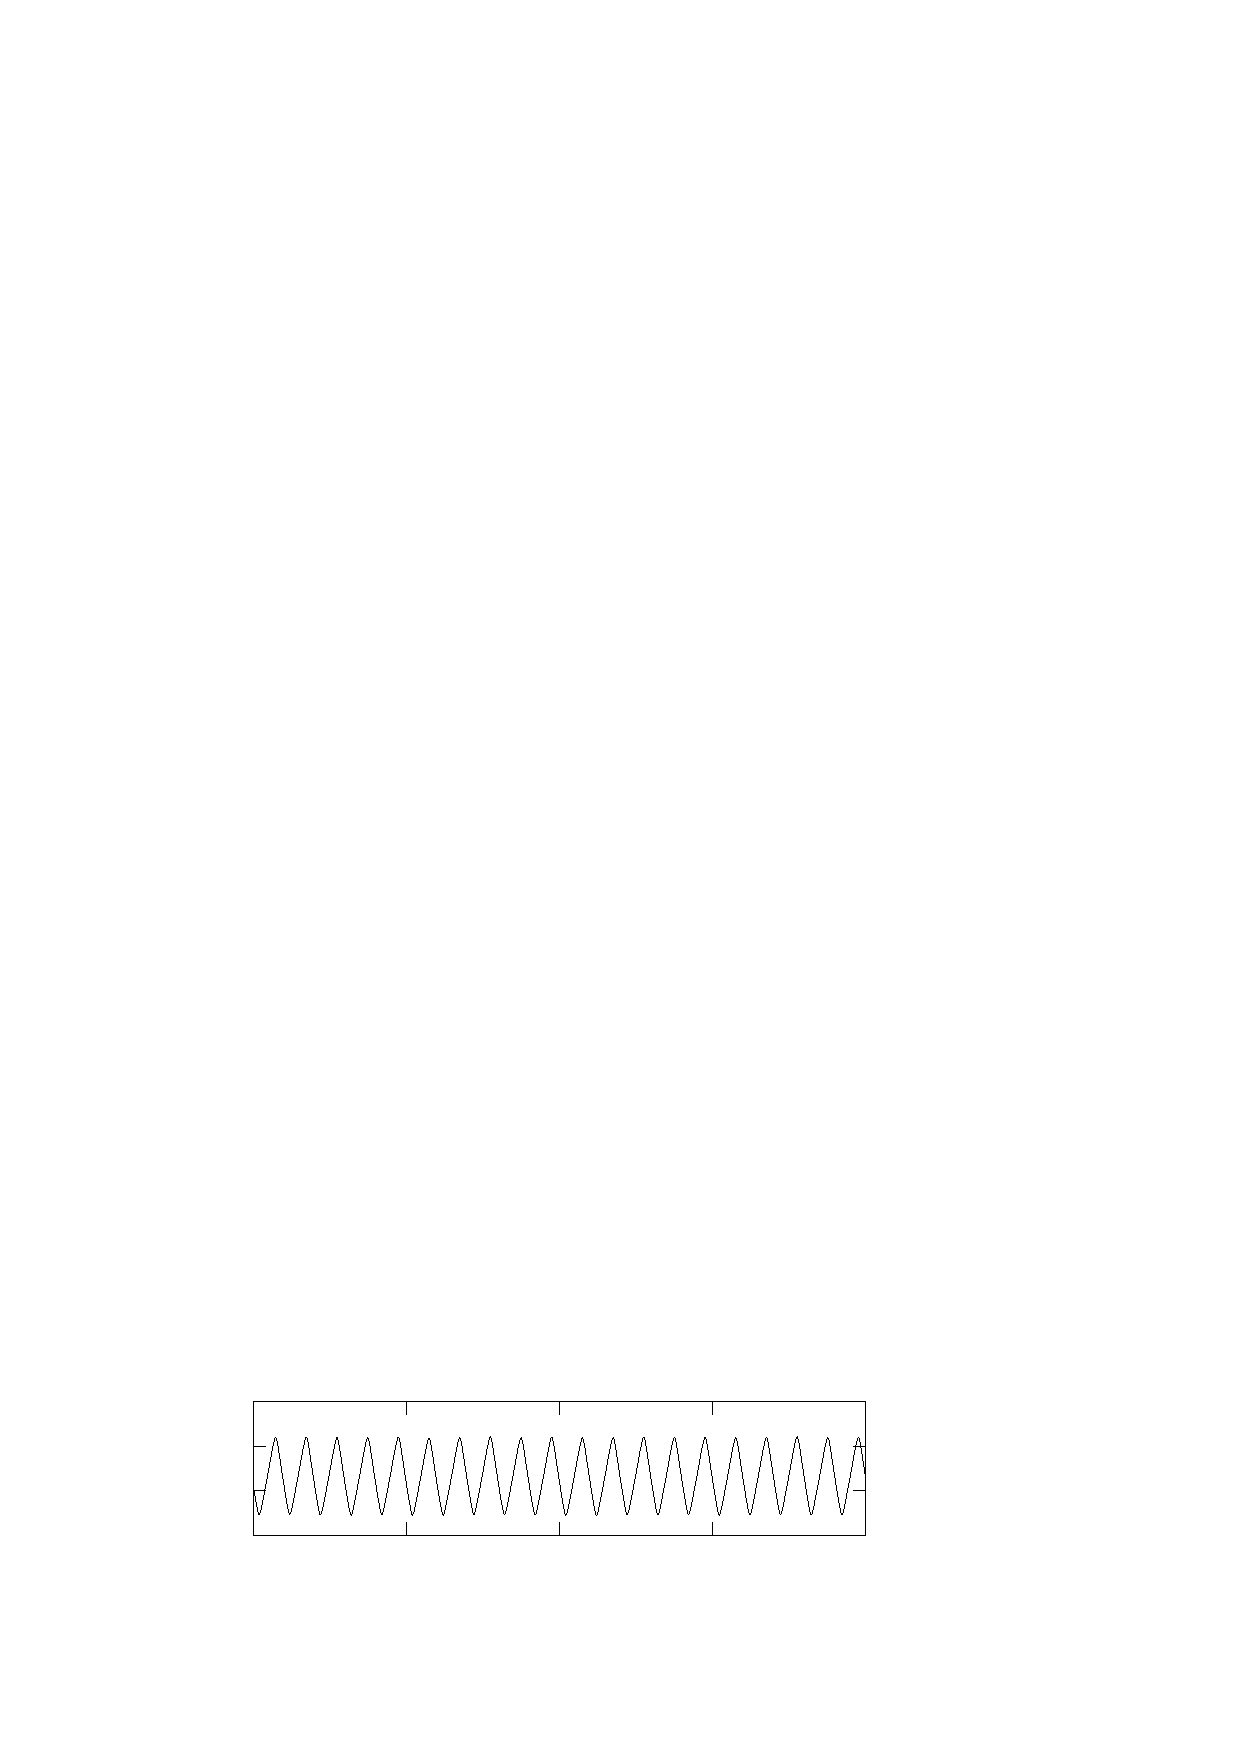
\includegraphics{rounded-barridorho1_2}%
%\end{picture}%
%\begingroup
%\setlength{\unitlength}{0.0200bp}%
%\begin{picture}(18000,5400)(0,0)%
%\put(2200,1650){\makebox(0,0)[r]{\strut{}1.26}}%
%\put(2200,2717){\makebox(0,0)[r]{\strut{}1.44}}%
%\put(2200,3783){\makebox(0,0)[r]{\strut{}1.62}}%
%\put(2200,4850){\makebox(0,0)[r]{\strut{}1.80}}%
%\put(2475,1100){\makebox(0,0){\strut{} 300}}%
%\put(6150,1100){\makebox(0,0){\strut{} 305}}%
%\put(9825,1100){\makebox(0,0){\strut{} 310}}%
%\put(13500,1100){\makebox(0,0){\strut{} 315}}%
%\put(17175,1100){\makebox(0,0){\strut{} 320}}%
%\put(550,3250){\rotatebox{90}{\makebox(0,0){\strut{}$y^\ast$}}}%
%\put(9825,275){\makebox(0,0){\strut{}$t^\ast$}}%
%\put(600,1000){\rotatebox{0}{\makebox(0,0){\strut{}(a)}}}%
%\end{picture}%
%\endgroup
%\endinput

%%GNUPLOT: LaTeX picture with Postscript
%\begin{picture}(0,0)%
%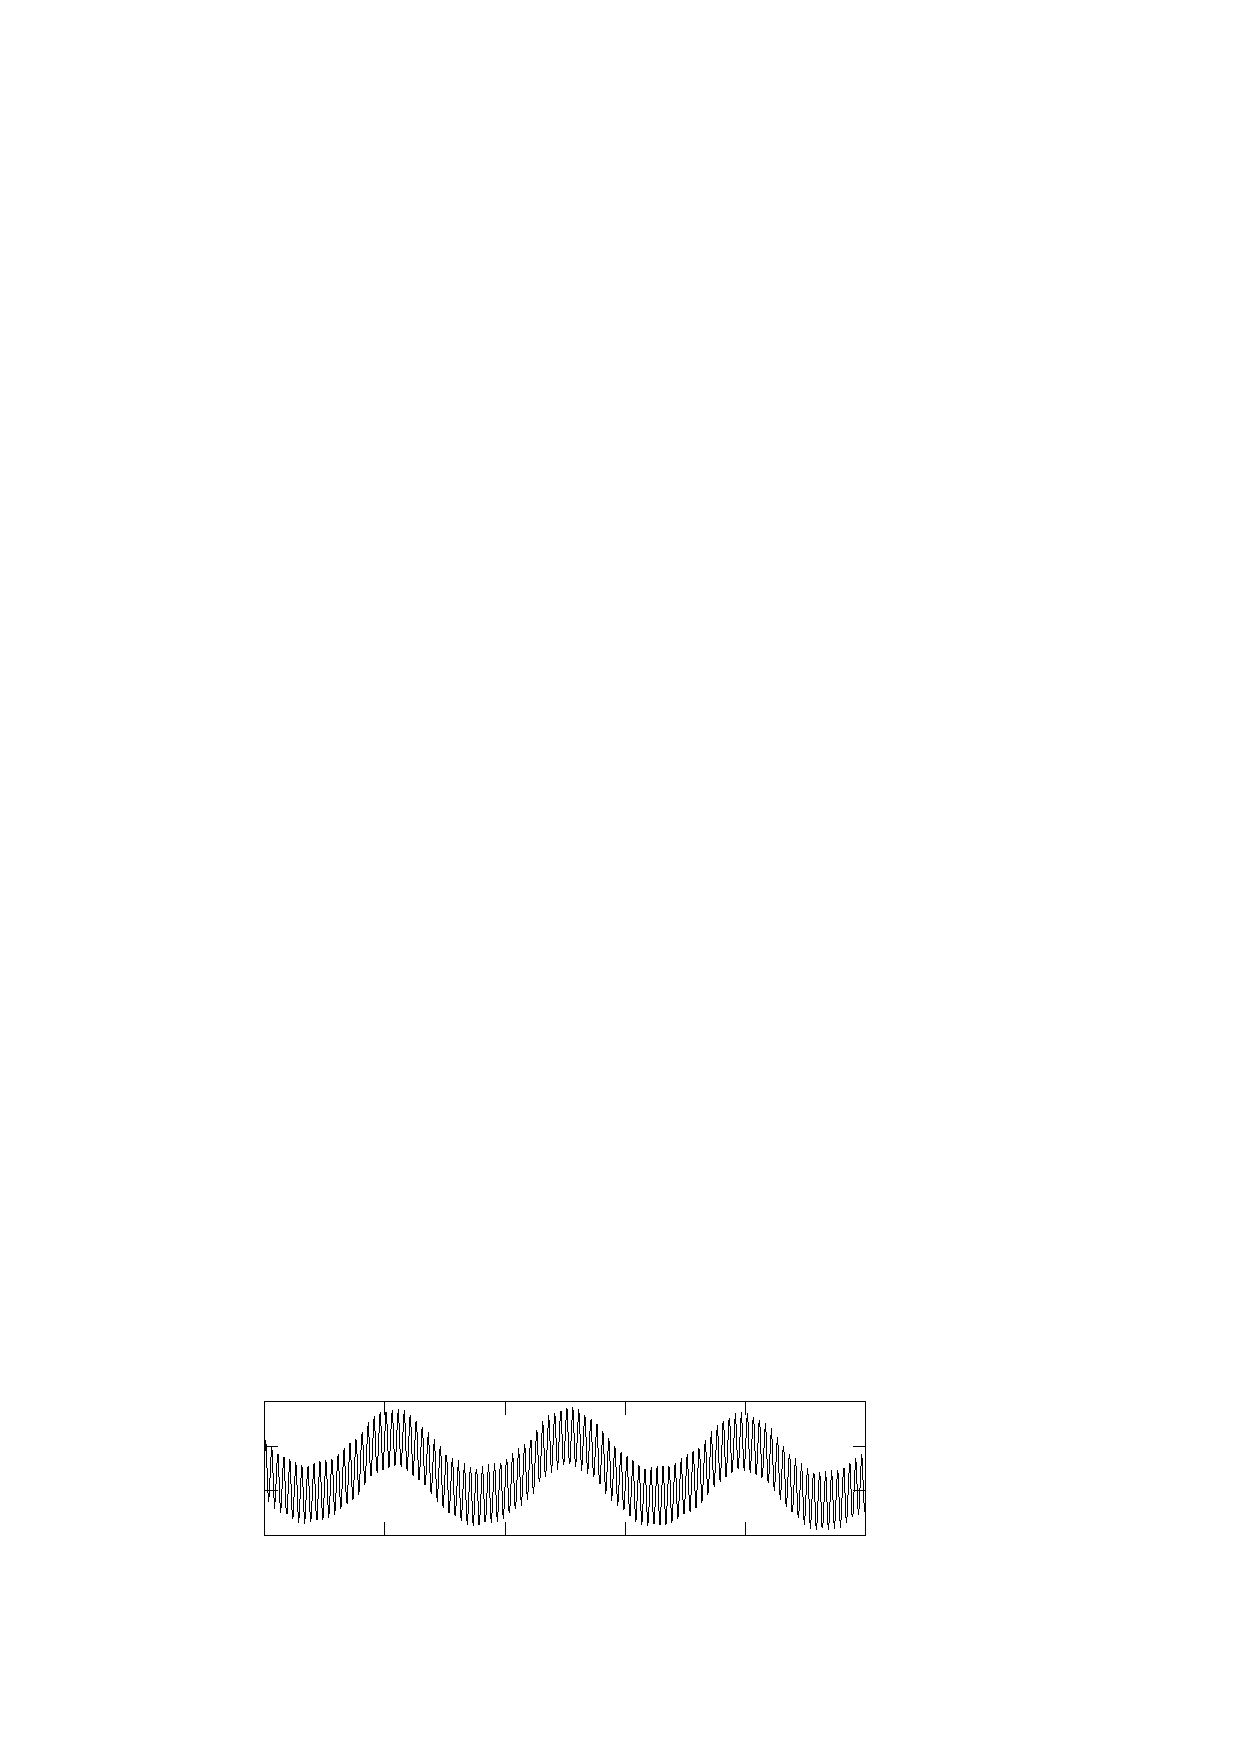
\includegraphics{rounded-barridorho30}%
%\end{picture}%
%\begingroup
%\setlength{\unitlength}{0.0200bp}%
%\begin{picture}(18000,5400)(0,0)%
%\put(2475,1650){\makebox(0,0)[r]{\strut{}1.410}}%
%\put(2475,2717){\makebox(0,0)[r]{\strut{}1.425}}%
%\put(2475,3783){\makebox(0,0)[r]{\strut{}1.440}}%
%\put(2475,4850){\makebox(0,0)[r]{\strut{}1.455}}%
%\put(2750,1100){\makebox(0,0){\strut{} 1800}}%
%\put(5635,1100){\makebox(0,0){\strut{} 1820}}%
%\put(8520,1100){\makebox(0,0){\strut{} 1840}}%
%\put(11405,1100){\makebox(0,0){\strut{} 1860}}%
%\put(14290,1100){\makebox(0,0){\strut{} 1880}}%
%\put(17175,1100){\makebox(0,0){\strut{} 1900}}%
%\put(550,3250){\rotatebox{90}{\makebox(0,0){\strut{}$y^\ast$}}}%
%\put(9962,275){\makebox(0,0){\strut{}$t^\ast$}}%
%\put(600,1000){\rotatebox{0}{\makebox(0,0){\strut{}(b)}}}%
%\end{picture}%
%\endgroup
%\endinput

%%GNUPLOT: LaTeX picture with Postscript
%\begin{picture}(0,0)%
%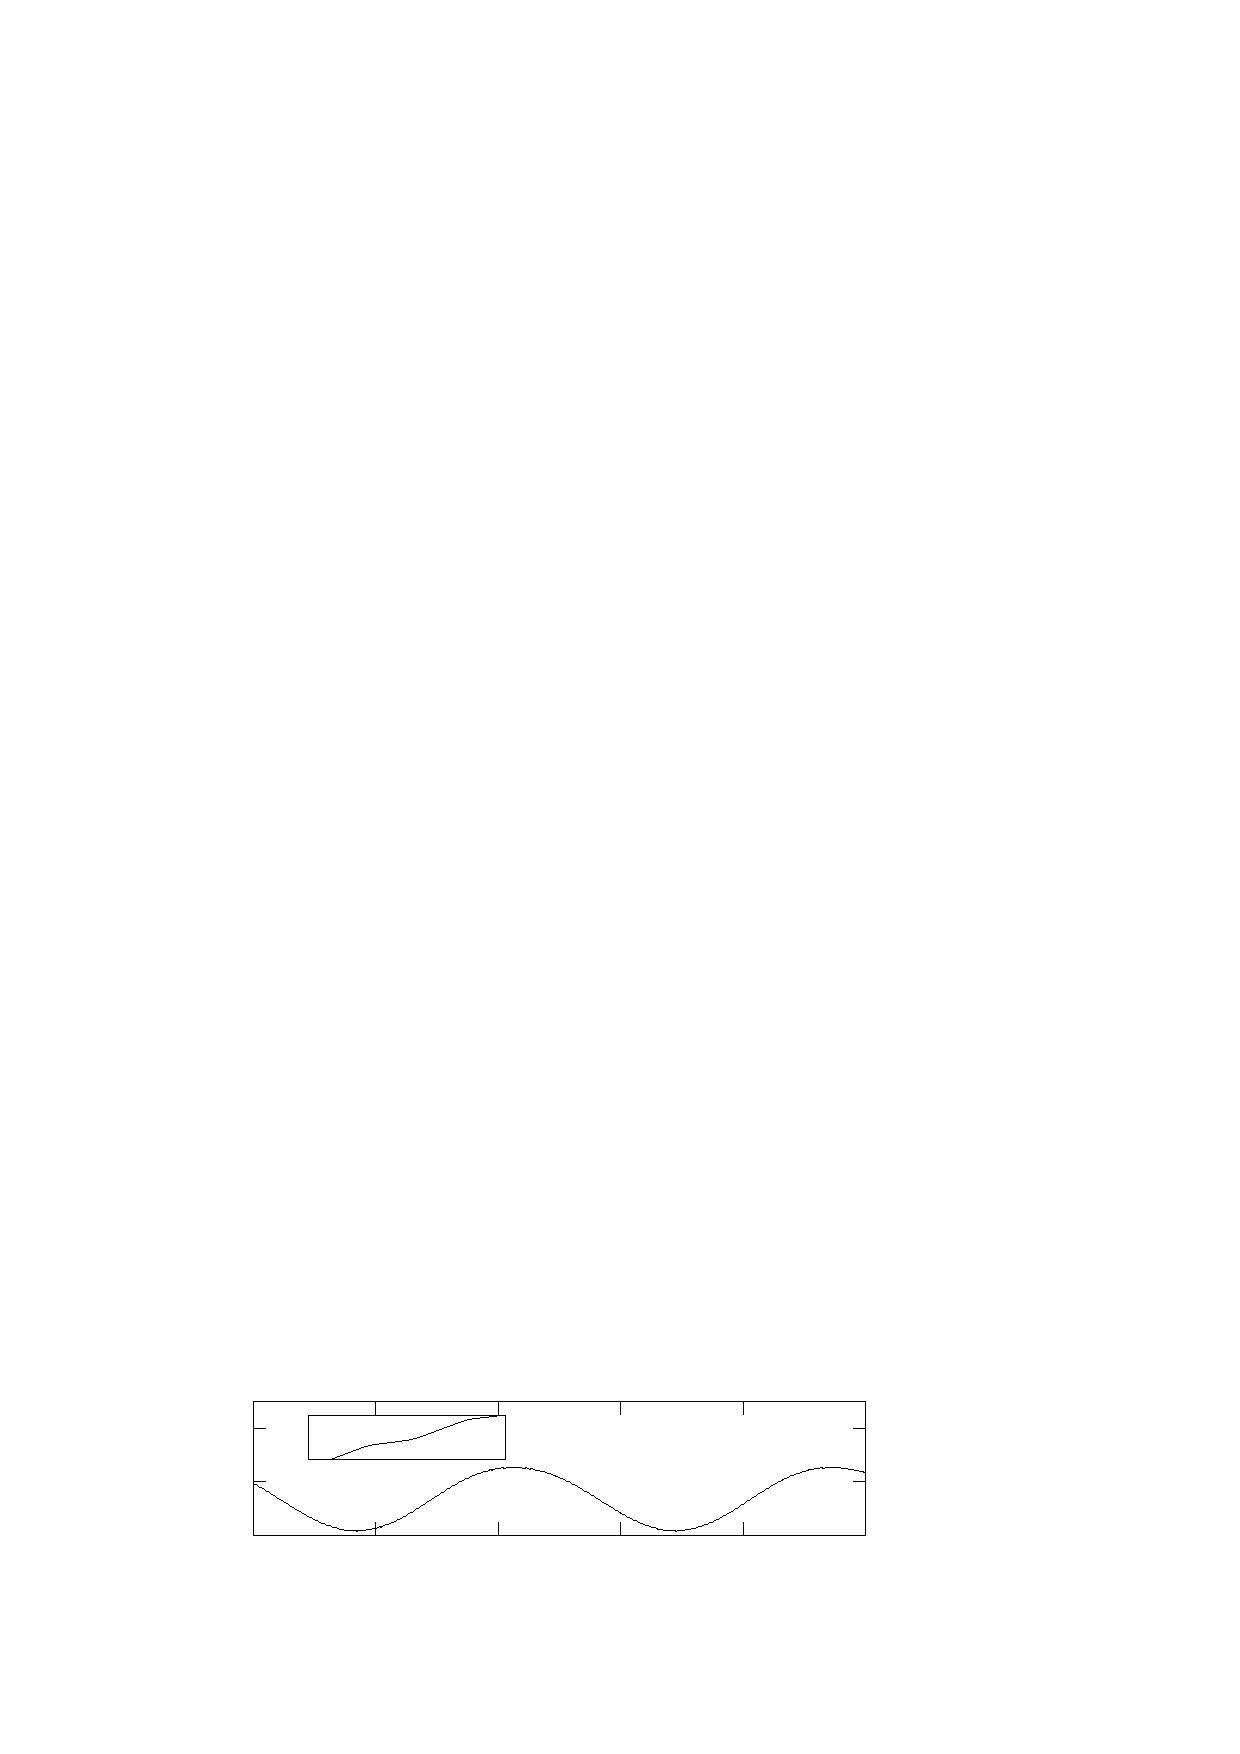
\includegraphics{rounded-barridorho60}%
%\end{picture}%
%\begingroup
%\setlength{\unitlength}{0.0200bp}%
%\begin{picture}(18000,5400)(0,0)%
%\put(2200,1650){\makebox(0,0)[r]{\strut{}0.80}}%
%\put(2200,2930){\makebox(0,0)[r]{\strut{}1.60}}%
%\put(2200,4210){\makebox(0,0)[r]{\strut{}2.40}}%
%\put(2475,1100){\makebox(0,0){\strut{} 1400}}%
%\put(5415,1100){\makebox(0,0){\strut{} 1420}}%
%\put(8355,1100){\makebox(0,0){\strut{} 1440}}%
%\put(11295,1100){\makebox(0,0){\strut{} 1460}}%
%\put(14235,1100){\makebox(0,0){\strut{} 1480}}%
%\put(17175,1100){\makebox(0,0){\strut{} 1500}}%
%\put(550,3250){\rotatebox{90}{\makebox(0,0){\strut{}$y^\ast$}}}%
%\put(9825,275){\makebox(0,0){\strut{}$t^\ast$}}%
%\put(3535,3476){\makebox(0,0)[r]{\strut{}1.4}}%
%\put(3535,4526){\makebox(0,0)[r]{\strut{}1.5}}%
%\put(3810,2926){\makebox(0,0){\strut{} 1430}}%
%\put(8535,2926){\makebox(0,0){\strut{} 1432}}%
%\put(600,1000){\rotatebox{0}{\makebox(0,0){\strut{}(c)}}}%
%\end{picture}%
%\endgroup
%\endinput

%%GNUPLOT: LaTeX picture with Postscript
%\begin{picture}(0,0)%
%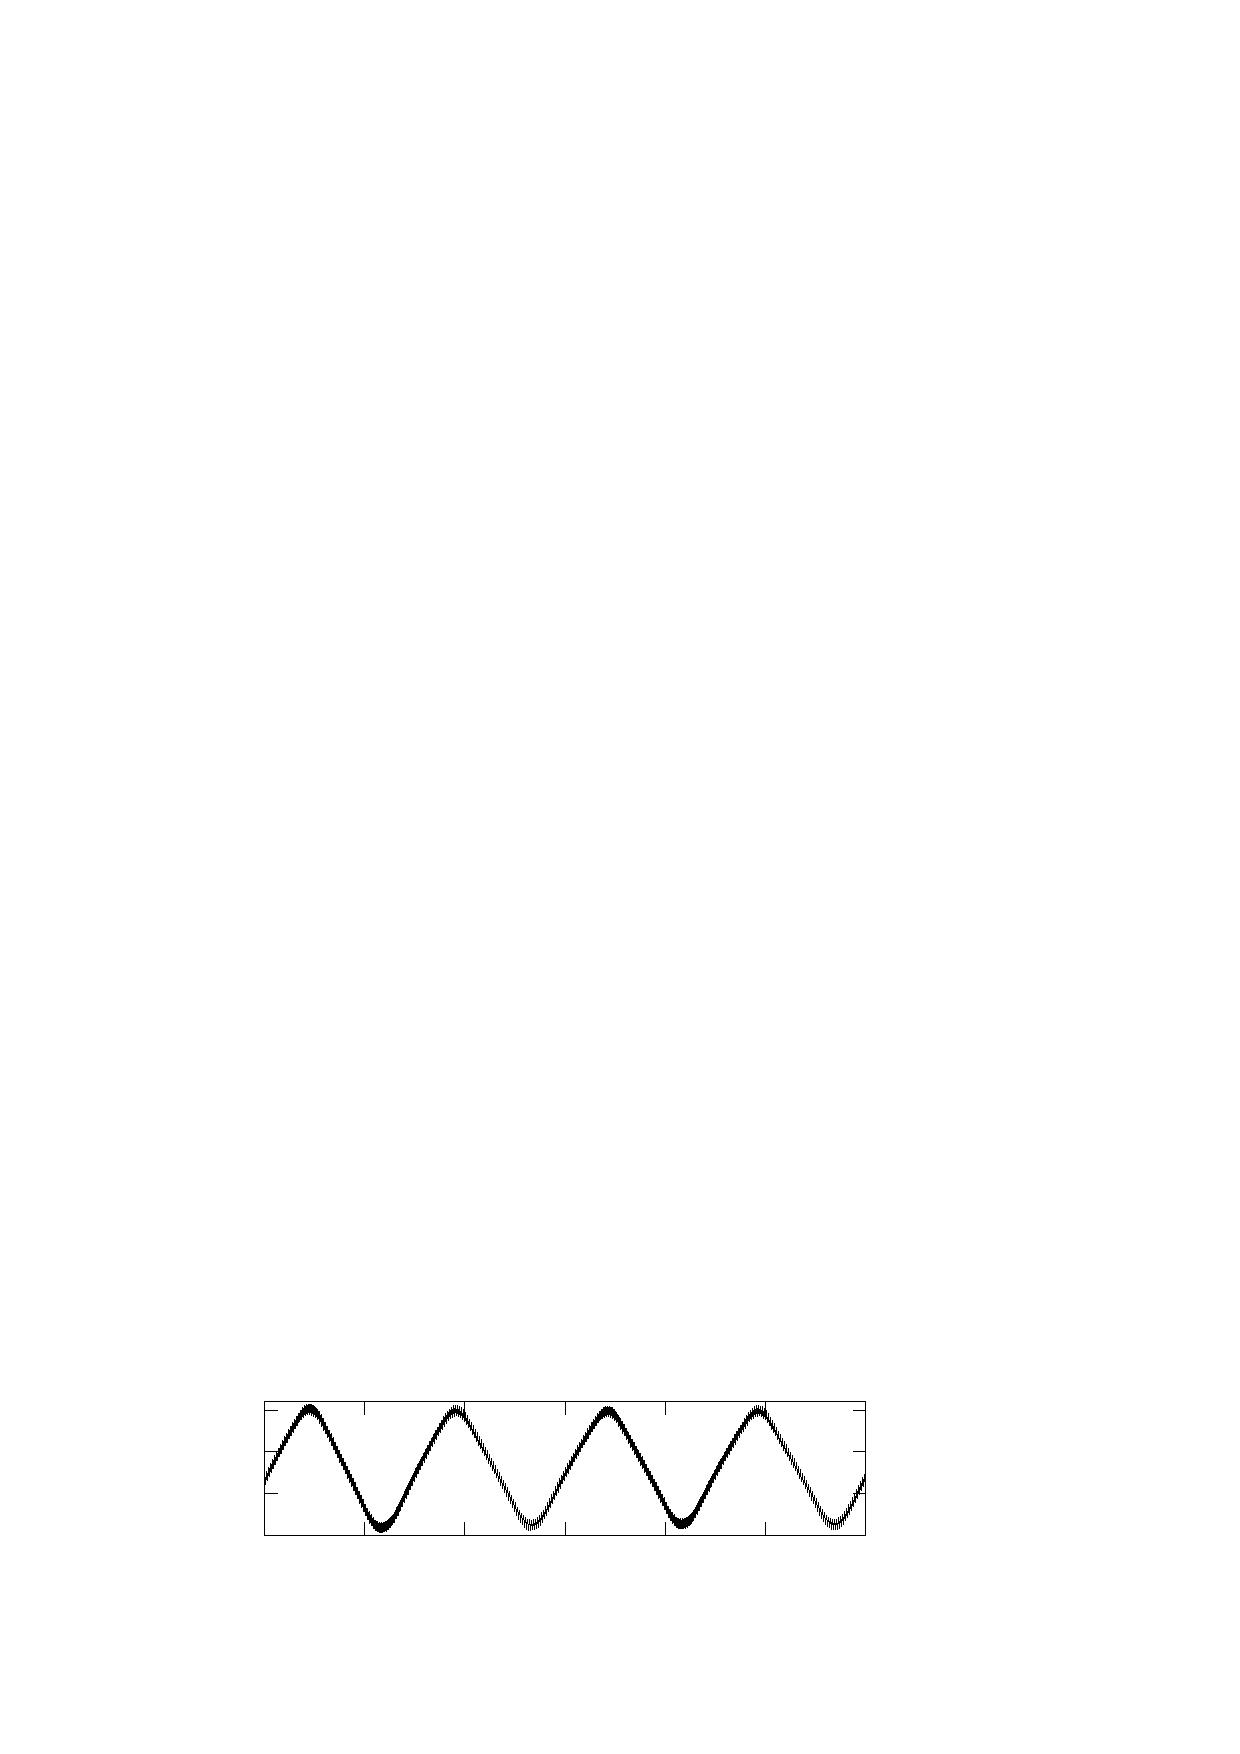
\includegraphics{rounded-barridorho153_6}%
%\end{picture}%
%\begingroup
%\setlength{\unitlength}{0.0200bp}%
%\begin{picture}(18000,5400)(0,0)%
%\put(2475,1650){\makebox(0,0)[r]{\strut{}1.020}}%
%\put(2475,2650){\makebox(0,0)[r]{\strut{}1.035}}%
%\put(2475,3650){\makebox(0,0)[r]{\strut{}1.050}}%
%\put(2475,4650){\makebox(0,0)[r]{\strut{}1.065}}%
%\put(2750,1100){\makebox(0,0){\strut{} 3000}}%
%\put(5154,1100){\makebox(0,0){\strut{} 3050}}%
%\put(7558,1100){\makebox(0,0){\strut{} 3100}}%
%\put(9963,1100){\makebox(0,0){\strut{} 3150}}%
%\put(12367,1100){\makebox(0,0){\strut{} 3200}}%
%\put(14771,1100){\makebox(0,0){\strut{} 3250}}%
%\put(17175,1100){\makebox(0,0){\strut{} 3300}}%
%\put(550,3250){\rotatebox{90}{\makebox(0,0){\strut{}$y^\ast$}}}%
%\put(9962,275){\makebox(0,0){\strut{}$t^\ast$}}%
%\put(600,1000){\makebox(0,0){\strut{}(d)}}%
%\end{picture}%
%\endgroup
%\endinput

\caption{\label{fig:paths-rounded}
Trayectoria de la posici'on vertical de la part'icula s'olida sobre el tiempo en la cavidad redondeada para
(a) $\rho_p/\rho_f = 2$,
(b) $\rho_p/\rho_f = 50$,
(c) $\rho_p/\rho_f = 100$
y
(d) $\rho_p/\rho_f =256$.
}
\end{figure}

\begin{figure}
%\put(600,2550){\rotatebox{90}{\makebox(0,0){\strut{}(a)}}}%
%%GNUPLOT: LaTeX picture with Postscript
%\begin{picture}(0,0)%
%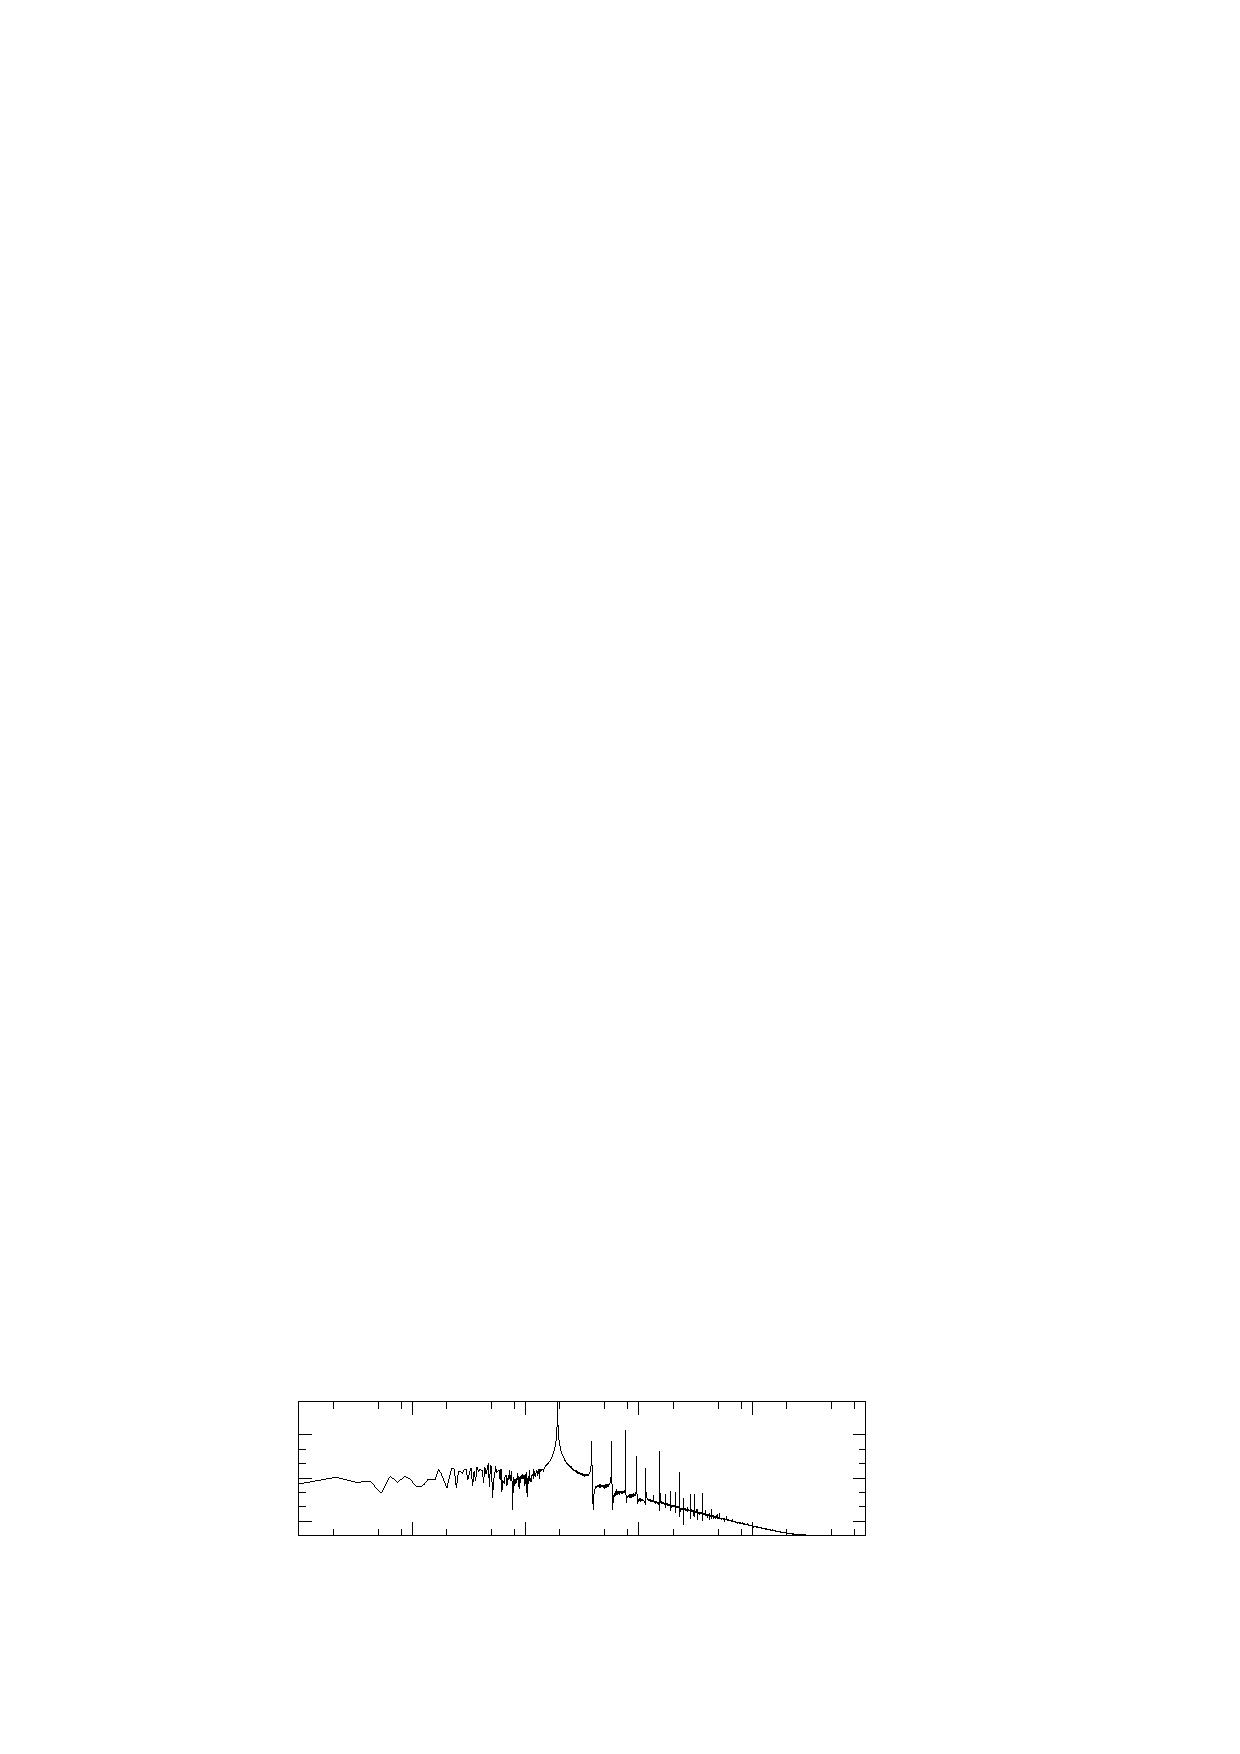
\includegraphics{rounded-barridorho1_2-spectrum}%
%\end{picture}%
%\begingroup
%\setlength{\unitlength}{0.0200bp}%
%\begin{picture}(18000,5400)(0,0)%
%\put(3300,1985){\makebox(0,0)[r]{\strut{}1.00e-12}}%
%\put(3300,3023){\makebox(0,0)[r]{\strut{}1.00e-09}}%
%\put(3300,4062){\makebox(0,0)[r]{\strut{}1.00e-06}}%
%\put(3575,1100){\makebox(0,0){\strut{} 1e-04}}%
%\put(6295,1100){\makebox(0,0){\strut{} 0.001}}%
%\put(9015,1100){\makebox(0,0){\strut{} 0.01}}%
%\put(11735,1100){\makebox(0,0){\strut{} 0.1}}%
%\put(14455,1100){\makebox(0,0){\strut{} 1}}%
%\put(17175,1100){\makebox(0,0){\strut{} 10}}%
%\put(550,3250){\rotatebox{90}{\makebox(0,0){\strut{}$PSD$}}}%
%\put(10375,275){\makebox(0,0){\strut{}$\omega$}}%
%\put(600,1000){\makebox(0,0){\strut{}(a)}}%
%\end{picture}%
%\endgroup
%\endinput

%%GNUPLOT: LaTeX picture with Postscript
%\begin{picture}(0,0)%
%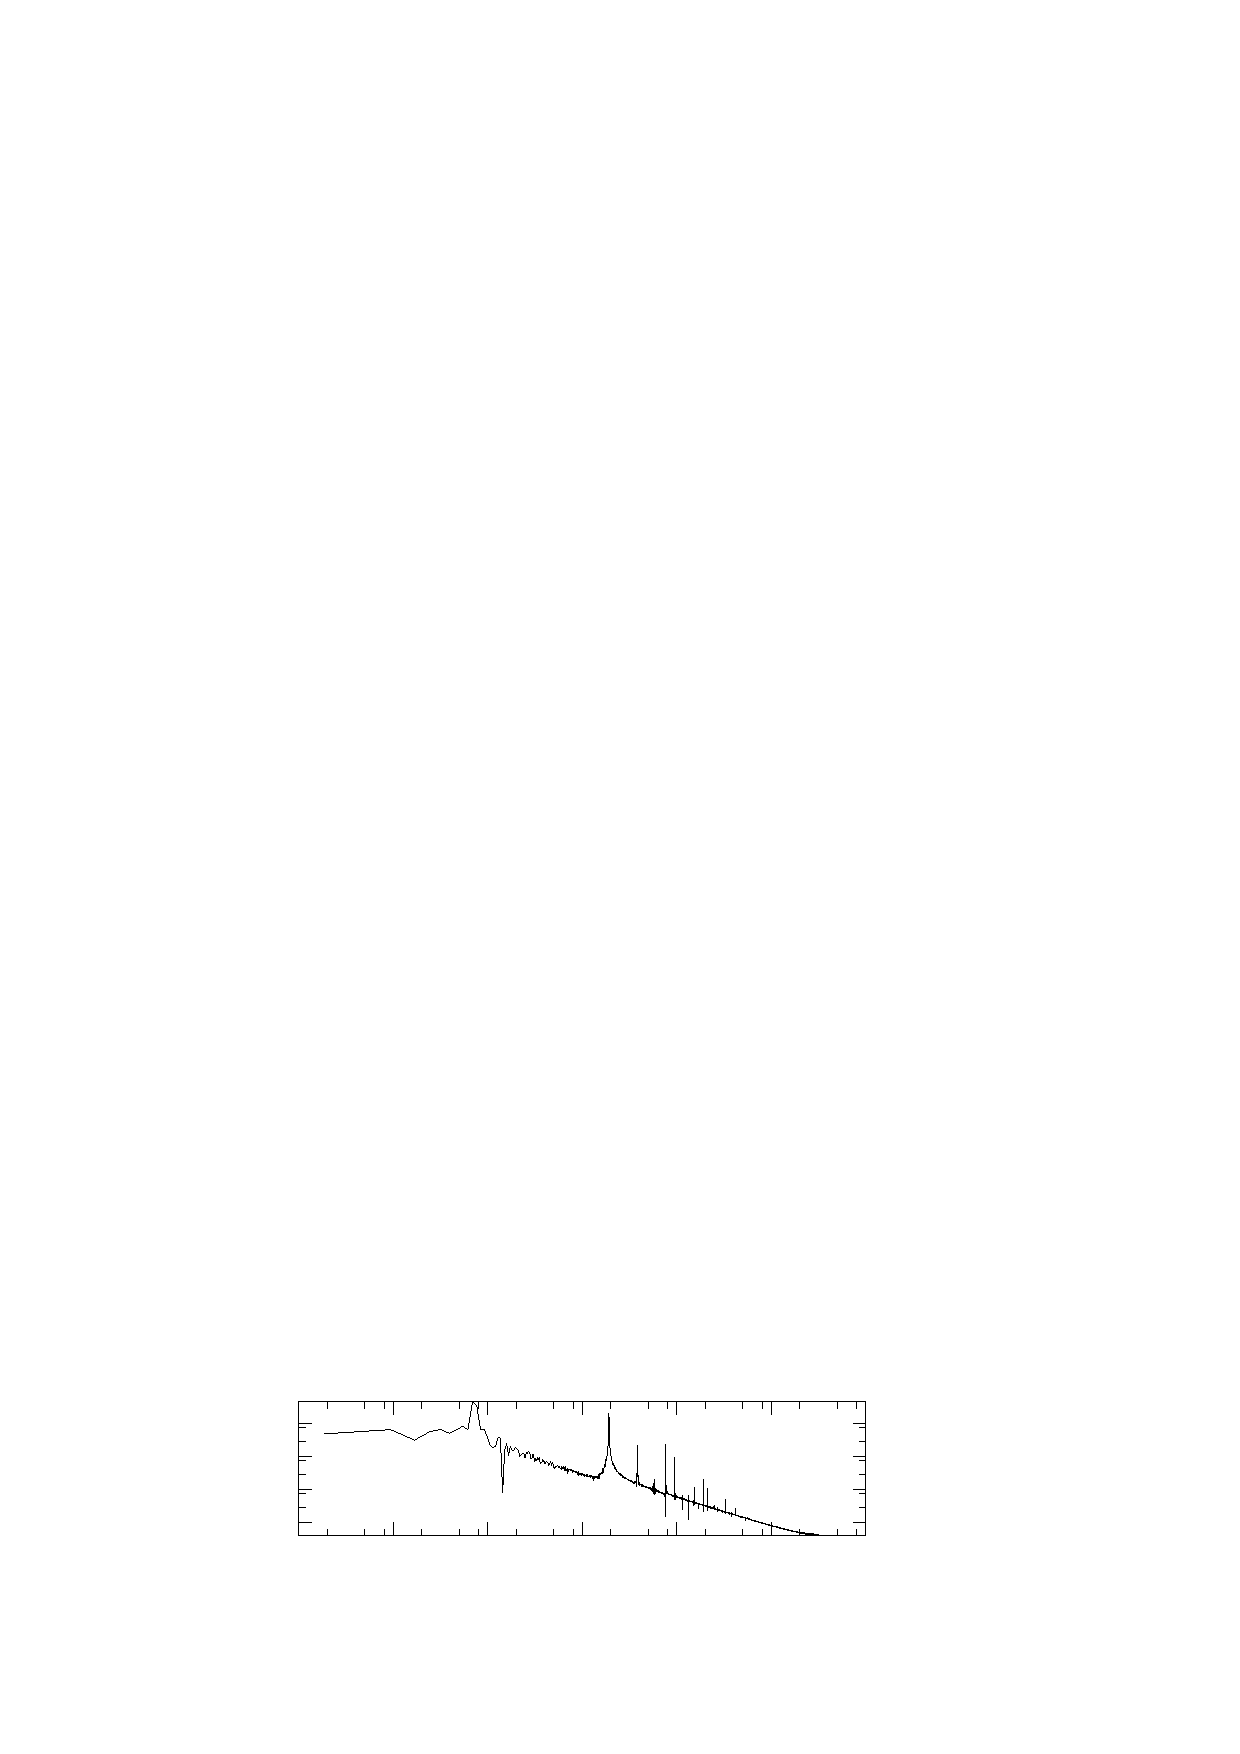
\includegraphics{rounded-barridorho30-spectrum}%
%\end{picture}%
%\begingroup
%\setlength{\unitlength}{0.0200bp}%
%\begin{picture}(18000,5400)(0,0)%
%\put(3300,1960){\makebox(0,0)[r]{\strut{}1.56e-14}}%
%\put(3300,2755){\makebox(0,0)[r]{\strut{}3.13e-12}}%
%\put(3300,3549){\makebox(0,0)[r]{\strut{}6.25e-10}}%
%\put(3300,4343){\makebox(0,0)[r]{\strut{}1.25e-07}}%
%\put(3575,1100){\makebox(0,0){\strut{} 1e-05}}%
%\put(5842,1100){\makebox(0,0){\strut{} 1e-04}}%
%\put(8108,1100){\makebox(0,0){\strut{} 0.001}}%
%\put(10375,1100){\makebox(0,0){\strut{} 0.01}}%
%\put(12642,1100){\makebox(0,0){\strut{} 0.1}}%
%\put(14908,1100){\makebox(0,0){\strut{} 1}}%
%\put(17175,1100){\makebox(0,0){\strut{} 10}}%
%\put(550,3250){\rotatebox{90}{\makebox(0,0){\strut{}$PSD$}}}%
%\put(10375,275){\makebox(0,0){\strut{}$\omega$}}%
%\put(600,1000){\makebox(0,0){\strut{}(b)}}%
%\end{picture}%
%\endgroup
%\endinput

%%GNUPLOT: LaTeX picture with Postscript
%\begin{picture}(0,0)%
%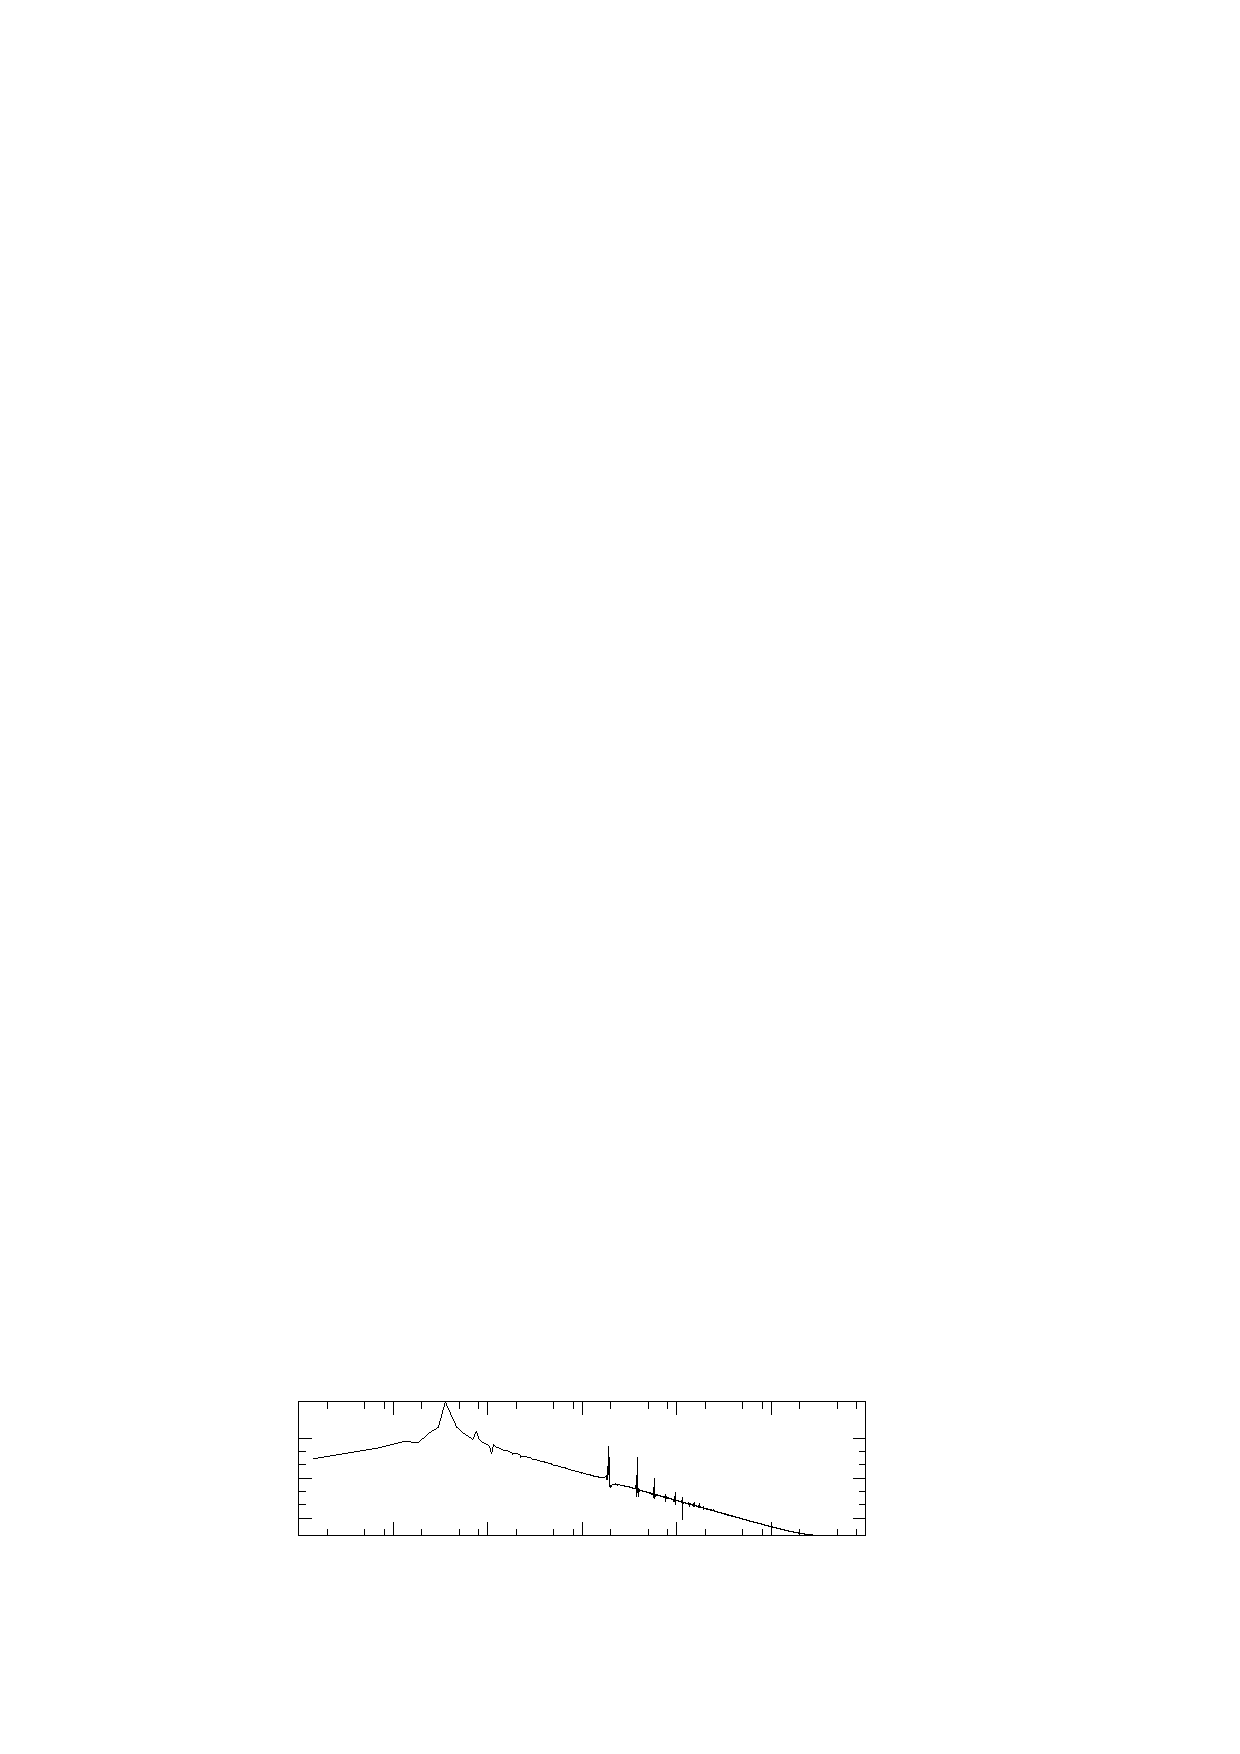
\includegraphics{rounded-barridorho60-spectrum}%
%\end{picture}%
%\begingroup
%\setlength{\unitlength}{0.0200bp}%
%\begin{picture}(18000,5400)(0,0)%
%\put(3300,2056){\makebox(0,0)[r]{\strut{}1.00e-12}}%
%\put(3300,3019){\makebox(0,0)[r]{\strut{}1.00e-09}}%
%\put(3300,3982){\makebox(0,0)[r]{\strut{}1.00e-06}}%
%\put(3575,1100){\makebox(0,0){\strut{} 1e-05}}%
%\put(5842,1100){\makebox(0,0){\strut{} 1e-04}}%
%\put(8108,1100){\makebox(0,0){\strut{} 0.001}}%
%\put(10375,1100){\makebox(0,0){\strut{} 0.01}}%
%\put(12642,1100){\makebox(0,0){\strut{} 0.1}}%
%\put(14908,1100){\makebox(0,0){\strut{} 1}}%
%\put(17175,1100){\makebox(0,0){\strut{} 10}}%
%\put(550,3250){\rotatebox{90}{\makebox(0,0){\strut{}$PSD$}}}%
%\put(10375,275){\makebox(0,0){\strut{}$\omega$}}%
%\put(600,1000){\makebox(0,0){\strut{}(c)}}%
%\end{picture}%
%\endgroup
%\endinput

%%GNUPLOT: LaTeX picture with Postscript
%\begin{picture}(0,0)%
%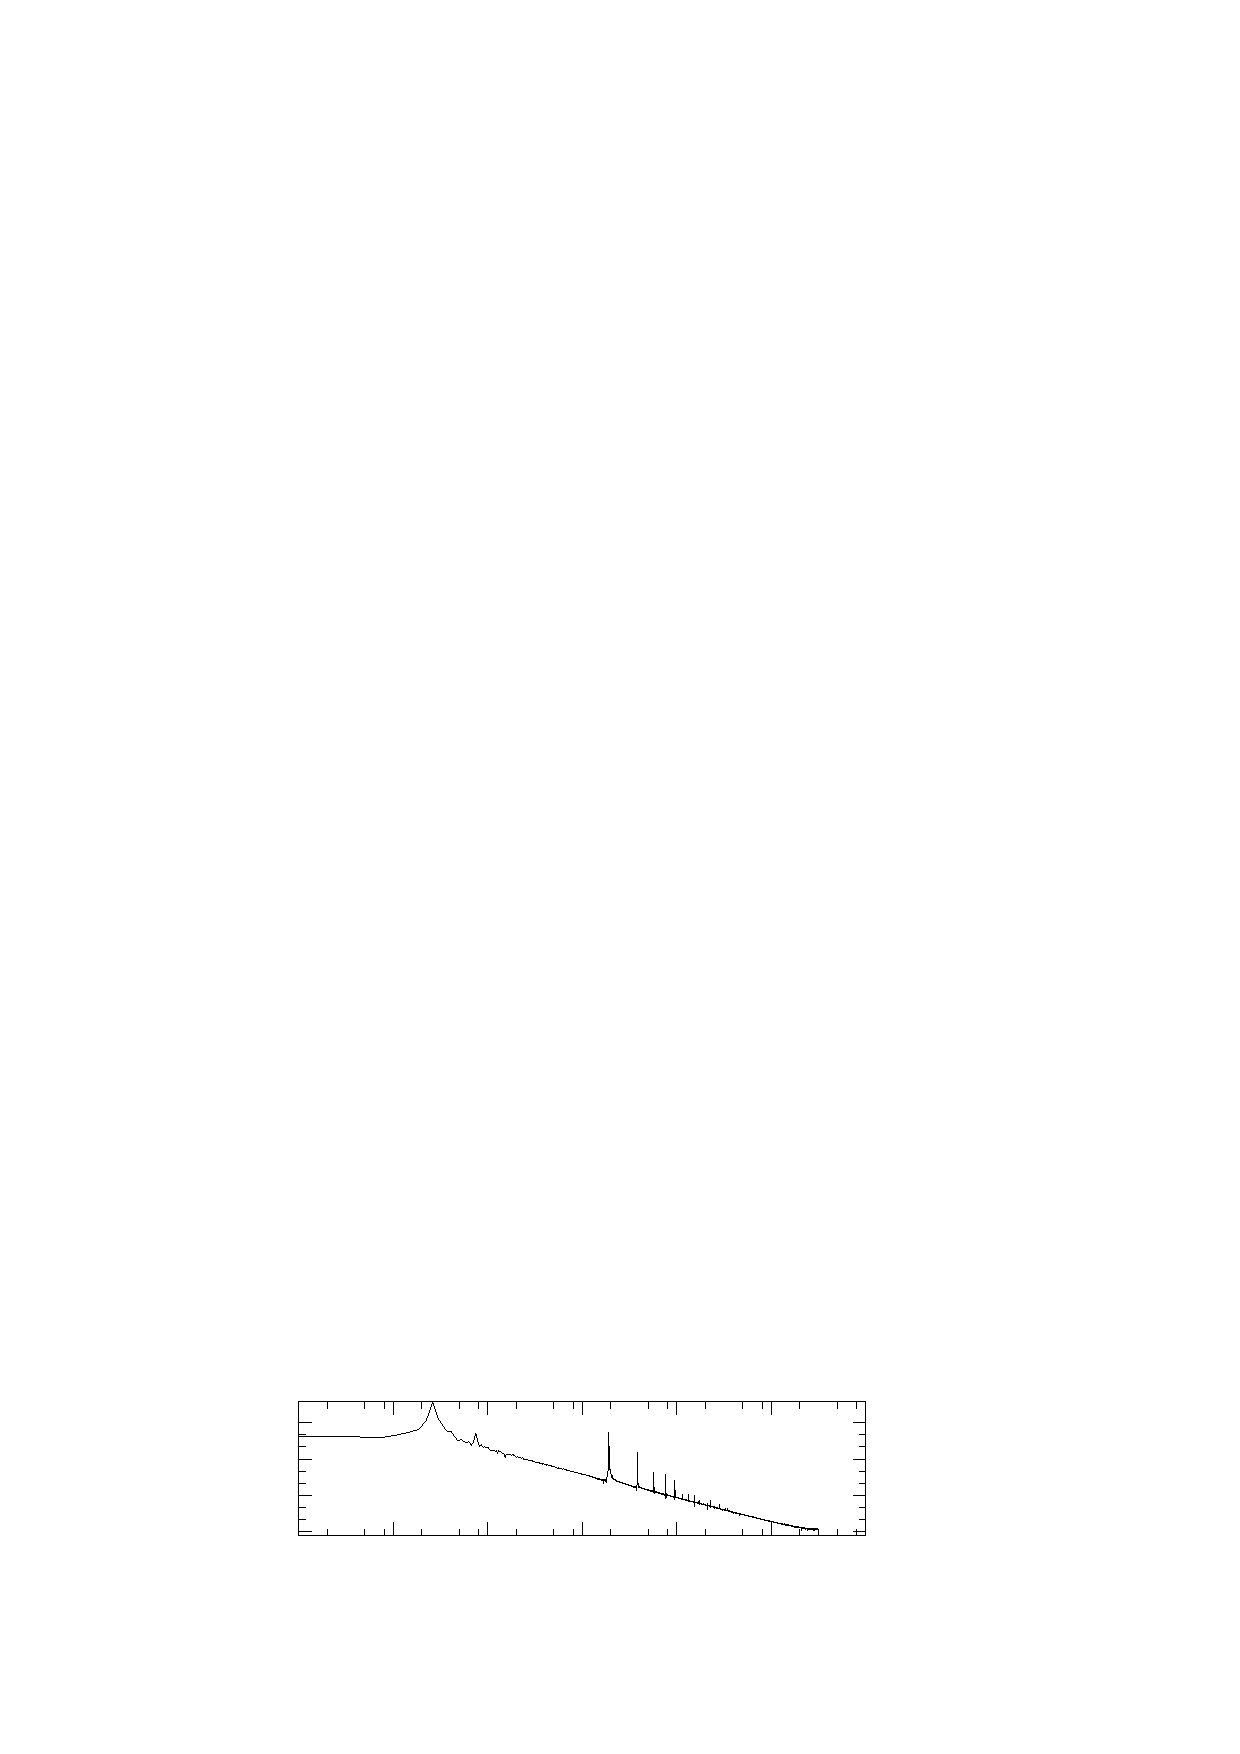
\includegraphics{rounded-barridorho153_6-spectrum}%
%\end{picture}%
%\begingroup
%\setlength{\unitlength}{0.0200bp}%
%\begin{picture}(18000,5400)(0,0)%
%\put(3300,1729){\makebox(0,0)[r]{\strut{}1.00e-15}}%
%\put(3300,2605){\makebox(0,0)[r]{\strut{}1.00e-12}}%
%\put(3300,3480){\makebox(0,0)[r]{\strut{}1.00e-09}}%
%\put(3300,4356){\makebox(0,0)[r]{\strut{}1.00e-06}}%
%\put(3575,1100){\makebox(0,0){\strut{} 1e-05}}%
%\put(5842,1100){\makebox(0,0){\strut{} 1e-04}}%
%\put(8108,1100){\makebox(0,0){\strut{} 0.001}}%
%\put(10375,1100){\makebox(0,0){\strut{} 0.01}}%
%\put(12642,1100){\makebox(0,0){\strut{} 0.1}}%
%\put(14908,1100){\makebox(0,0){\strut{} 1}}%
%\put(17175,1100){\makebox(0,0){\strut{} 10}}%
%\put(550,3250){\rotatebox{90}{\makebox(0,0){\strut{}$PSD$}}}%
%\put(600,1000){\makebox(0,0){\strut{}(d)}}%
%\end{picture}%
%\endgroup
%\endinput

\caption{\label{fig:spectrum-rounded}
Espectro de potencia del movimiento vertical de la part'icula s'olida sobre el tiempo en la cavidad redondeada para
(a) $\rho_p/\rho_f = 2$,
(b) $\rho_p/\rho_f = 50$,
(c) $\rho_p/\rho_f = 100$
y
(d) $\rho_p/\rho_f =256$.
Los espectros de potencia corresponden a los de las figuras~\ref{fig:paths-rounded} (a), (b), (c) y (d). 
}
\end{figure}

La cavidad redondeada presenta un comportamiento m'as complejo que la plana. 
En las figuras~\ref{fig:paths-rounded} (a), (b), (c) y (d) se muestran cuatro variantes
del comportamiento de la part'icula s'olida. En la figura~\ref{fig:paths-rounded} (a) para 
$\rho_p/\rho_f = 2$, el movimiento de la part'icula es simple, se mueve con la misma
frecuencia que la fuente ac'ustica y la desviaci'on est'andard es $\sigma_y=0.10$. En 
la figura~\ref{fig:paths-rounded} (b)  para $\rho_p/\rho_f = 50$ aparece una segunda frecuencia
y la oscilaci'on se reduce $\sigma_y=0.009$ por un orden de magnitud. Cuando la desviaci'on
est'andard casi alcanza su m'aximo $\sigma_y = 0.34$, la amplitud de la oscilaci'on debida 
a la fuente ac'ustica casi desaparece, como se puede ver en el la figura~\ref{fig:paths-rounded} (c) 
y su inserto. Antes de que la densidad sea tan grande que la part'icula caiga, figura~\ref{fig:paths-rounded} (d),
el valor de la desviaci'on est'andard decrece a $\sigma_y=0.013$. En estas simulaciones num'ericas,
el movimiento de la part'icula alcanz'o valores de $\sigma_y$ m'as grandes que el radio de la misma $r^\ast = 0.25$.
En las figuras~\ref{fig:spectrum-rounded} (a), (b), (c) y (d) se muestran los espectros de
potencia de las trayectorias de las figuras~\ref{fig:paths-rounded} (a), (b), (c) y (d), respectivamente.
De estas figuras se confirma que el movimiento de la part'icula puede contener solamente a la 
frecuencia de la fuente ac'ustica y sus arm'onicos, figura~\ref{fig:spectrum-rounded} (a), o
contener una segunda frecuencia de oscilaci'on que se va haciendo m'as peque~na conforme la
densidad de la part'icula aumenta, acompa~nada tambi'en de sus arm'onicos, como se ve en 
en las figuras~\ref{fig:spectrum-rounded} (c) y (d).










\begin{figure}
%\put(3800,4350){\makebox(0,0)[r]{\strut{}(a)}}%
%GNUPLOT: LaTeX picture with Postscript
\begin{picture}(0,0)%
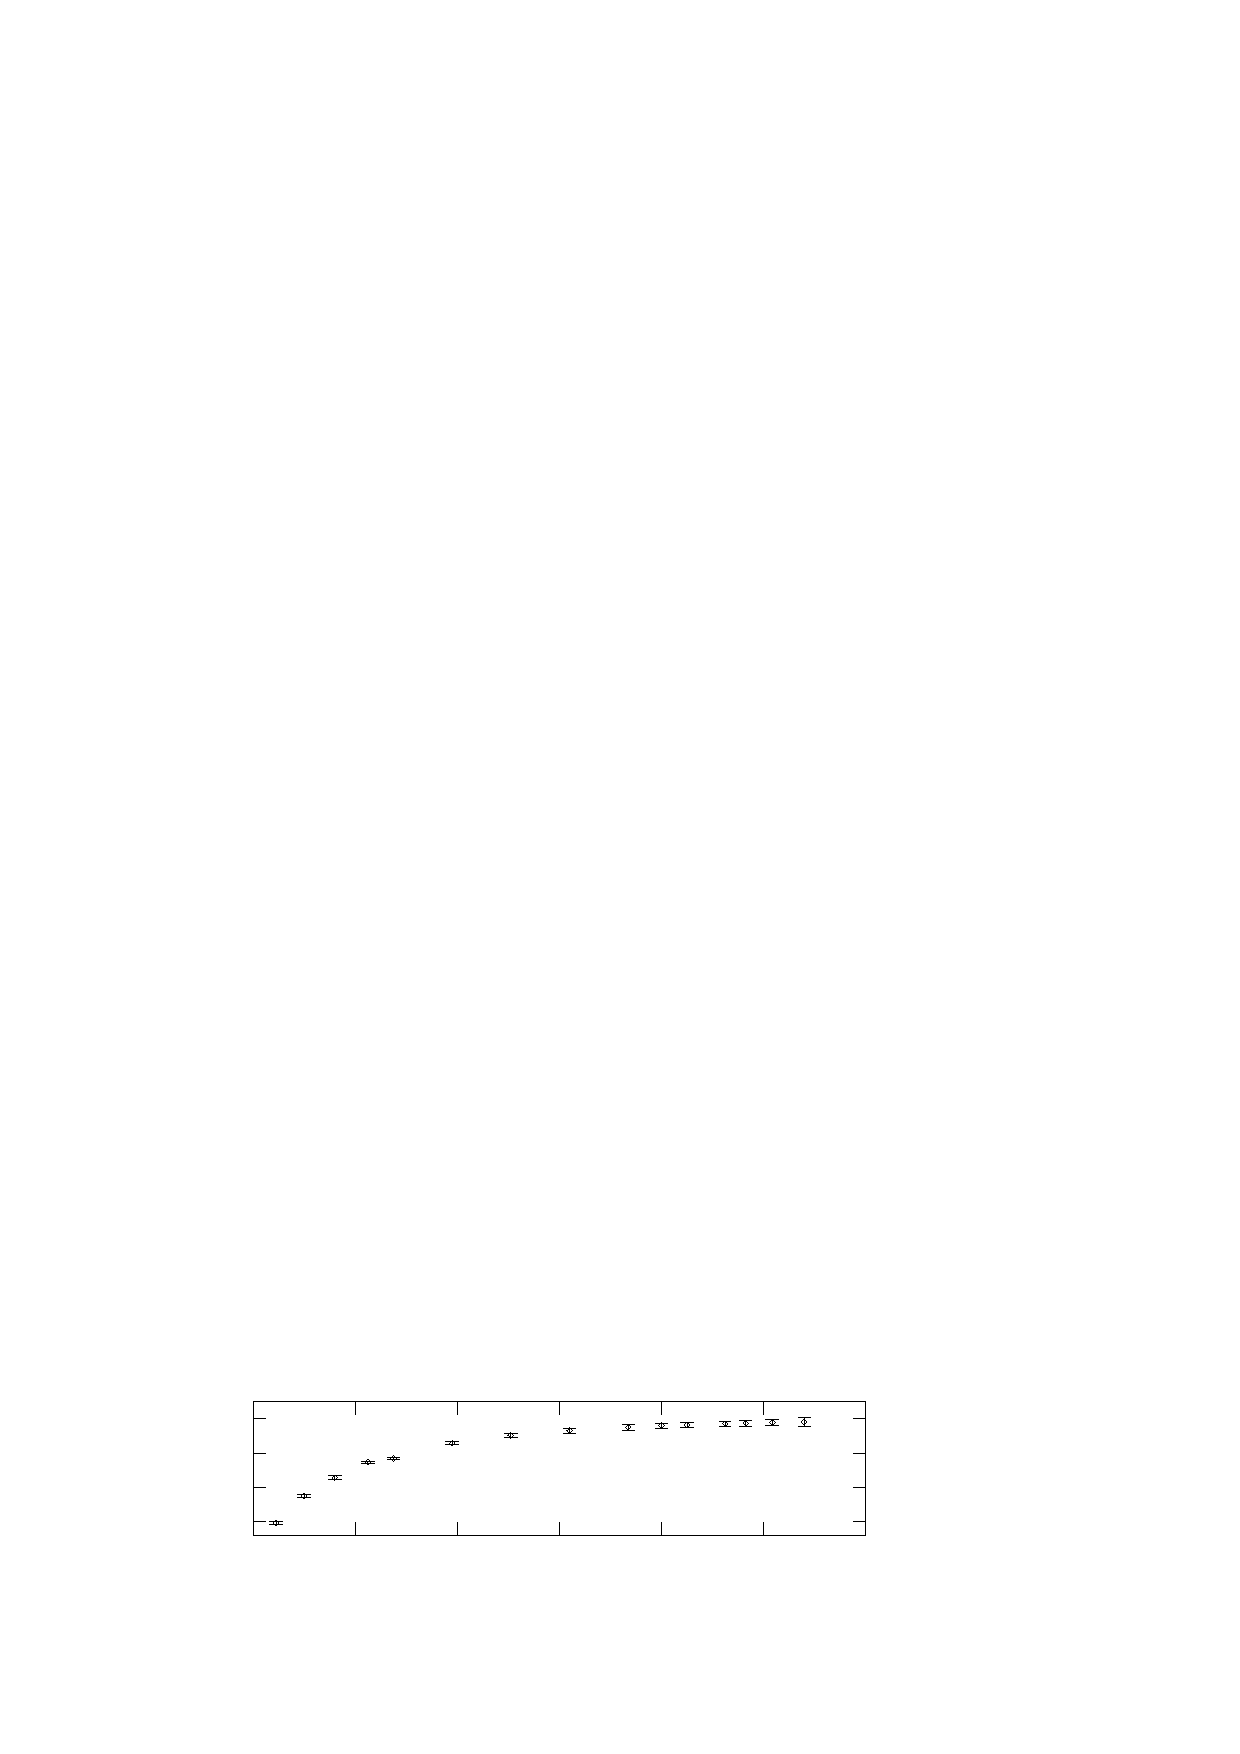
\includegraphics{eps/Fo-equilibrium-amplitud-flat}%
\end{picture}%
\begingroup
\setlength{\unitlength}{0.0200bp}%
\begin{picture}(18000,5400)(0,0)%
\put(2200,1990){\makebox(0,0)[r]{\strut{}1.20}}%
\put(2200,2807){\makebox(0,0)[r]{\strut{}1.32}}%
\put(2200,3624){\makebox(0,0)[r]{\strut{}1.44}}%
\put(2200,4441){\makebox(0,0)[r]{\strut{}1.56}}%
\put(2475,1100){\makebox(0,0){\strut{}0.004}}%
\put(4925,1100){\makebox(0,0){\strut{}0.006}}%
\put(7375,1100){\makebox(0,0){\strut{}0.008}}%
\put(9825,1100){\makebox(0,0){\strut{}0.010}}%
\put(12275,1100){\makebox(0,0){\strut{}0.012}}%
\put(14725,1100){\makebox(0,0){\strut{}0.014}}%
\put(17175,1100){\makebox(0,0){\strut{}0.016}}%
\put(550,3250){\rotatebox{90}{\makebox(0,0){\strut{}$y_{es}^\ast$}}}%
\put(9825,275){\makebox(0,0){\strut{}$P^\ast$}}%
\put(600,1000){\makebox(0,0)[r]{\strut{}(a)}}%
\end{picture}%
\endgroup
\endinput

%GNUPLOT: LaTeX picture with Postscript
\begin{picture}(0,0)%
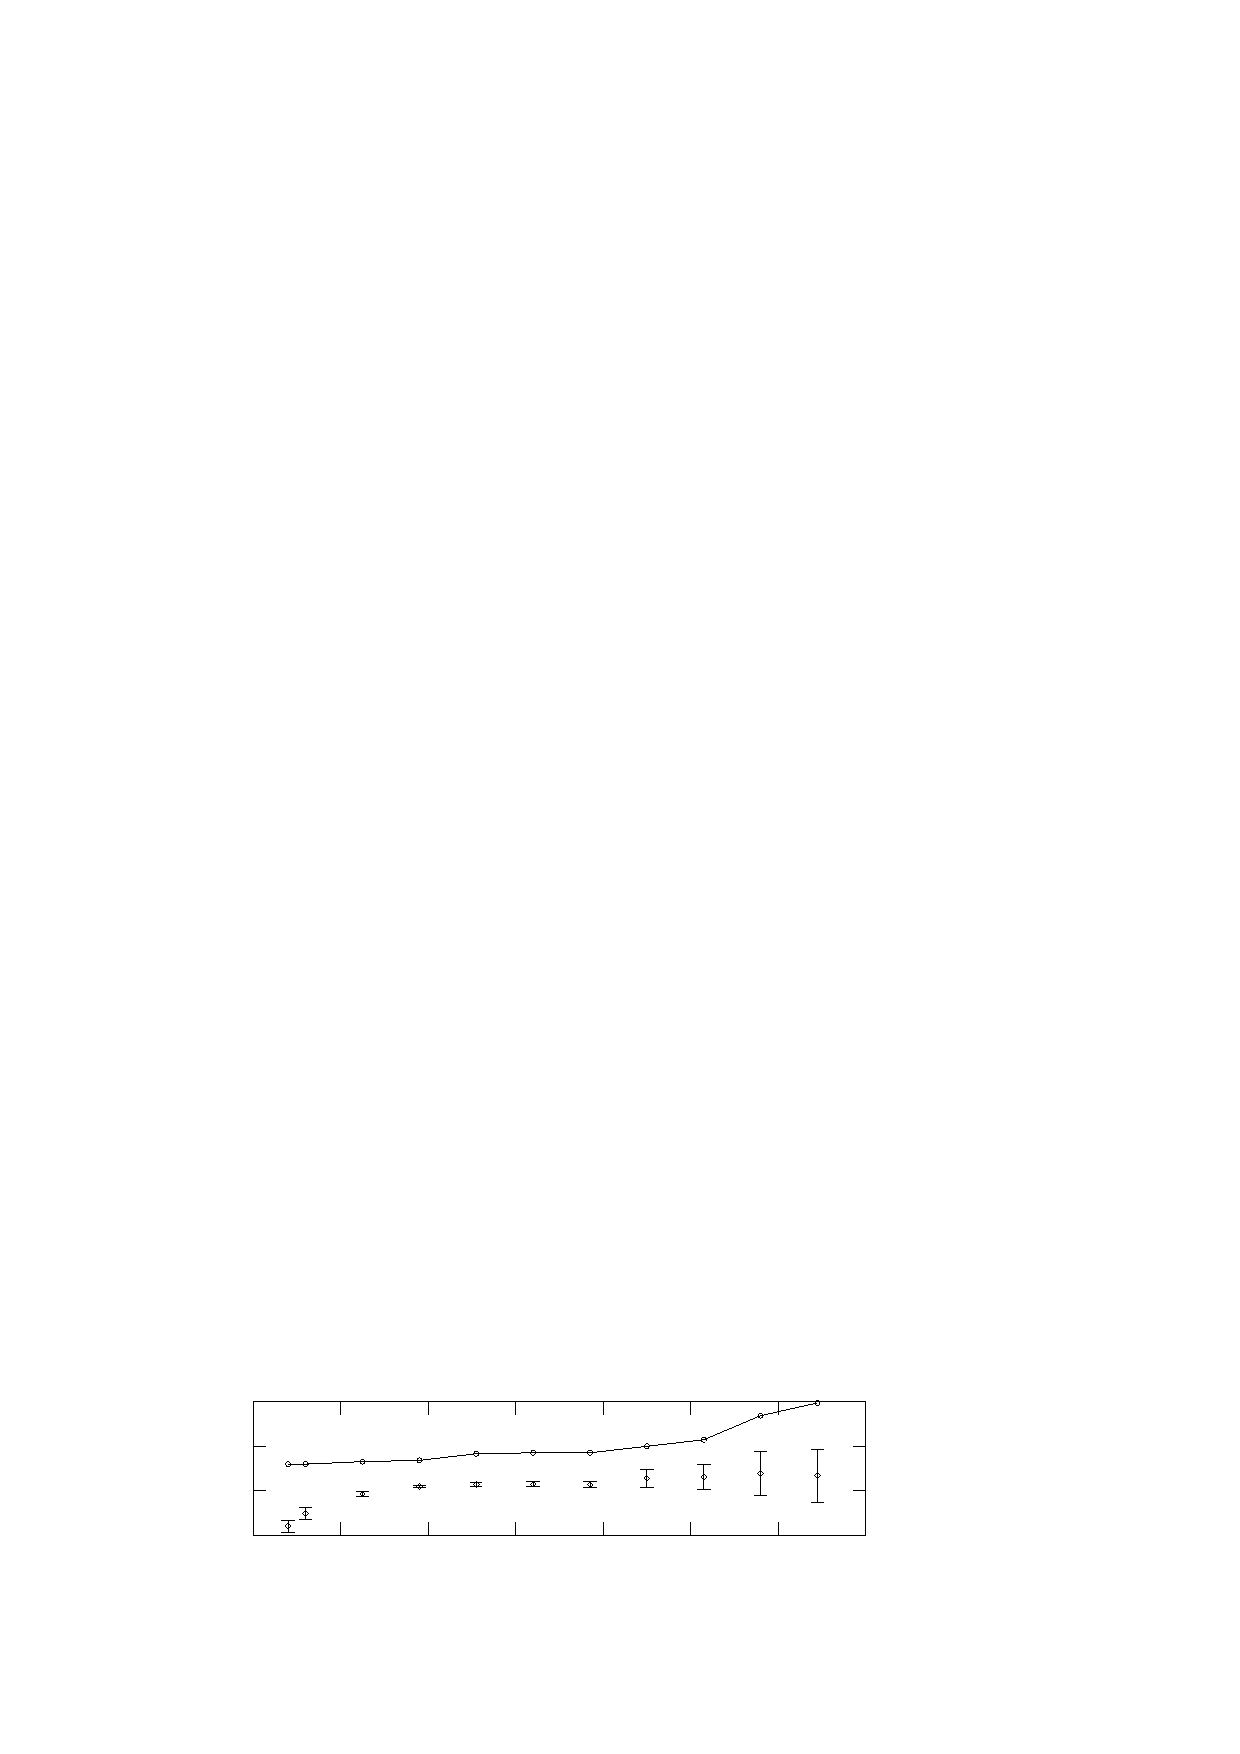
\includegraphics{Fo-equilibrium-amplitud-rounded}%
\end{picture}%
\begingroup
\setlength{\unitlength}{0.0200bp}%
\begin{picture}(18000,5400)(0,0)%
\put(2200,1650){\makebox(0,0)[r]{\strut{}1.05}}%
\put(2200,2717){\makebox(0,0)[r]{\strut{}1.40}}%
\put(2200,3783){\makebox(0,0)[r]{\strut{}1.75}}%
\put(2200,4850){\makebox(0,0)[r]{\strut{}2.10}}%
\put(2475,1100){\makebox(0,0){\strut{}0.000}}%
\put(4575,1100){\makebox(0,0){\strut{}0.001}}%
\put(6675,1100){\makebox(0,0){\strut{}0.002}}%
\put(8775,1100){\makebox(0,0){\strut{}0.003}}%
\put(10875,1100){\makebox(0,0){\strut{}0.004}}%
\put(12975,1100){\makebox(0,0){\strut{}0.005}}%
\put(15075,1100){\makebox(0,0){\strut{}0.006}}%
\put(17175,1100){\makebox(0,0){\strut{}0.007}}%
\put(550,3250){\rotatebox{90}{\makebox(0,0){\strut{}$y^\ast_{es}$}}}%
\put(9825,275){\makebox(0,0){\strut{}$P^\ast$}}%
\put(600,1000){\rotatebox{0}{\makebox(0,0){\strut{}(b)}}}%
\end{picture}%
\endgroup
\endinput

%%GNUPLOT: LaTeX picture with Postscript
%\begin{picture}(0,0)%
%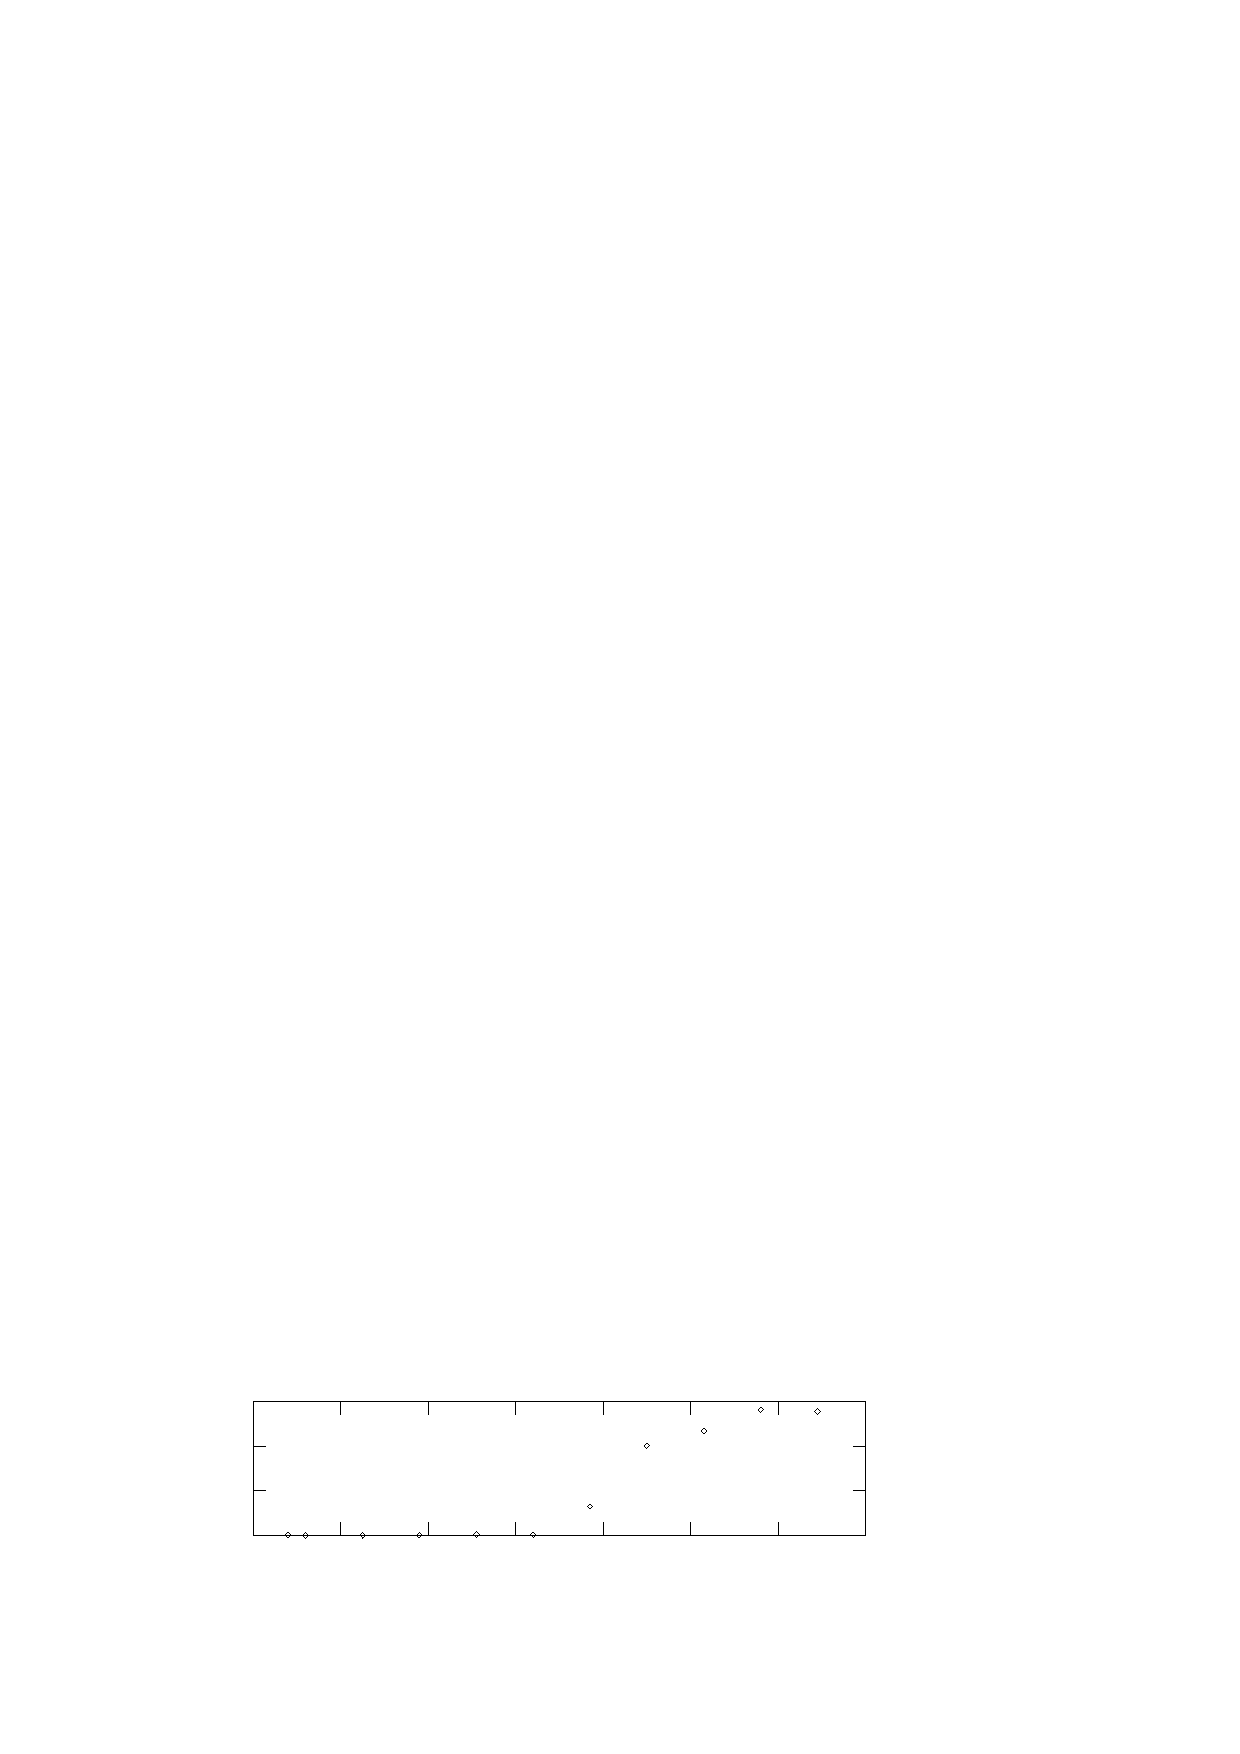
\includegraphics{Fo-equilibrium-amplitud-rounded-x}%
%\end{picture}%
%\begingroup
%\setlength{\unitlength}{0.0200bp}%
%\begin{picture}(18000,5400)(0,0)%
%\put(2200,1650){\makebox(0,0)[r]{\strut{}0.00}}%
%\put(2200,2717){\makebox(0,0)[r]{\strut{}0.50}}%
%\put(2200,3783){\makebox(0,0)[r]{\strut{}1.00}}%
%\put(2200,4850){\makebox(0,0)[r]{\strut{}1.50}}%
%\put(2475,1100){\makebox(0,0){\strut{}0.000}}%
%\put(4575,1100){\makebox(0,0){\strut{}0.001}}%
%\put(6675,1100){\makebox(0,0){\strut{}0.002}}%
%\put(8775,1100){\makebox(0,0){\strut{}0.003}}%
%\put(10875,1100){\makebox(0,0){\strut{}0.004}}%
%\put(12975,1100){\makebox(0,0){\strut{}0.005}}%
%\put(15075,1100){\makebox(0,0){\strut{}0.006}}%
%\put(17175,1100){\makebox(0,0){\strut{}0.007}}%
%\put(550,3250){\rotatebox{90}{\makebox(0,0){\strut{}$\sigma_x^\ast$}}}%
%\put(9825,275){\makebox(0,0){\strut{}$P_o^\ast$}}%
%\put(600,1000){\rotatebox{0}{\makebox(0,0){\strut{}(c)}}}%
%\end{picture}%
%\endgroup
%\endinput

\caption{\label{fig:barrido-momento}
Posici'on de equilibrio y desviaci'on est'andar como funci'on de la cantidad de movimiento
agregado  $P^\ast$ con 
$\rho_p/\rho_f=50$ para la cavidad  (a) plana  y (b) redondeada. Para  
$P_o^\ast>4\times 10^{-3}$ la part'icula comienza a oscilar horizontalmente, como se muestra en (c).
}
\end{figure}

En el siguiente conjunto de simulaciones num'ericas se mantuvo constante la
relaci'on de densidades en  $\rho_p/\rho_f=50$  en presencia de un campo
gravitacional externo y se vari'o la cantidad de movimiento
agregada por la fuente ac'ustica $P_o^\ast$  para la cavidad plana y
la redondeada. Como en el conjunto de simulaciones num'ericas anteriores, se midi'o la
posici'on de equilibrio y la desviaci'on est'andard alrededor de 'esta. 
En las figuras~\ref{fig:barrido-momento} (a) y (b) se muestra la posici'on de equilibrio
con la desviaci'on est'andard alrededor del eje vertical como funci'on de la cantidad
de movimiento para la cavidad plana y la redondeada, respectivamente. En la
figura~\ref{fig:barrido-momento} (c) se muestra la desviaci'on est'andard en el
eje horizontal para la part'icula  en la cavidad redondeada.  Conforme se aumenta la
cantidad de movimiento agregada por la fuente ac'ustica, la part'icula es desplazada hacia
el nodo de presi'on, como se puede apreciar en la figura~\ref{fig:barrido-momento} (a), para
la cavidad plana. Tambi'en, conforme aumenta la cantidad de movimiento agregada aumenta
el valor de $\sigma_y$.  Para la part'icula en la cavidad redondeada, el punto de equilibrio
se desplaza hacia el nodo de presi'on conforme aumenta la cantidad de movimiento
agregada, pero para $P_o^\ast > 4\times 10^{-3}$ el desplazamiento ya no sigue la misma tendencia
y al mismo tiempo la part'icula comienza a oscilar tambi'en en el eje horizontal, como se puede
ver de la figura~\ref{fig:barrido-momento} (c). 



\begin{figure}
%\put(600,2550){\rotatebox{90}{\makebox(0,0){\strut{}(a)}}}%
%%GNUPLOT: LaTeX picture with Postscript
%\begin{picture}(0,0)%
%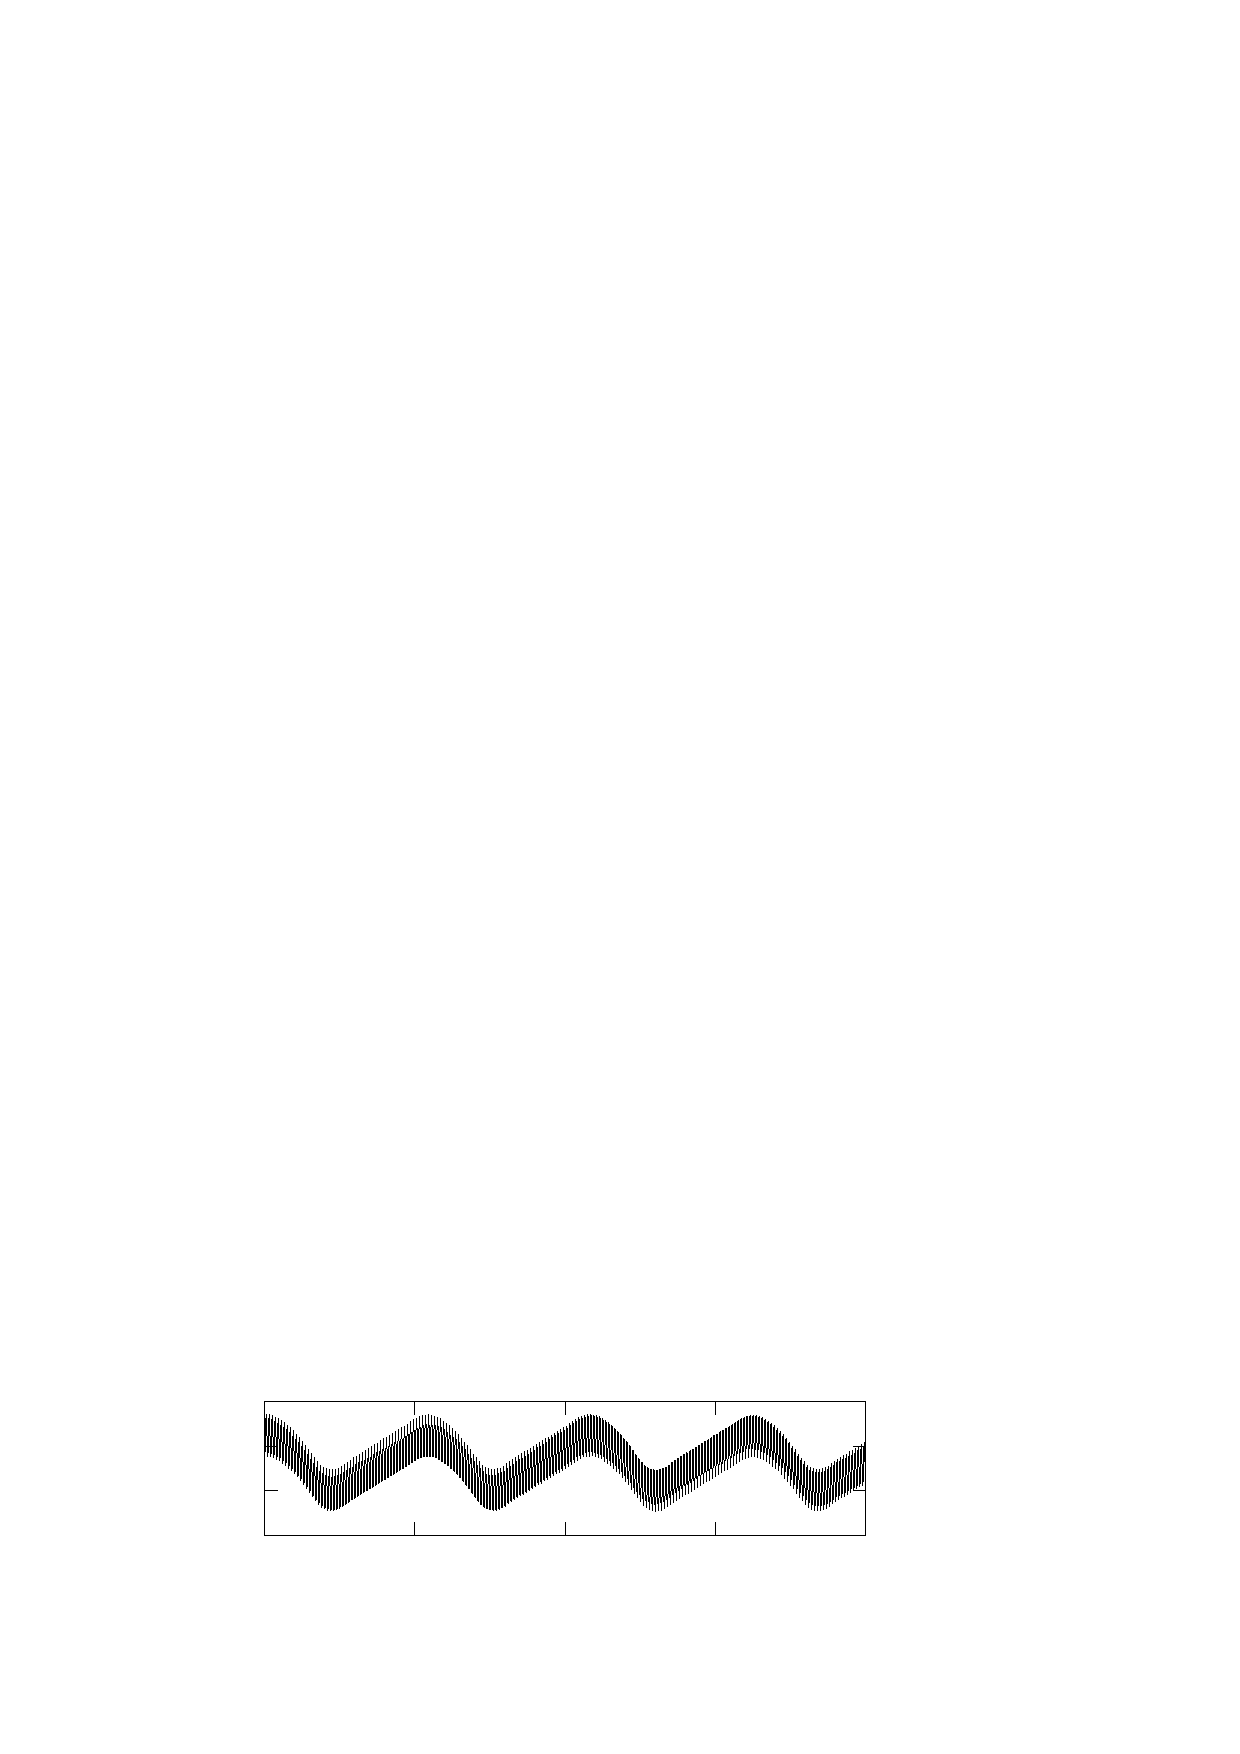
\includegraphics{flat-rho-30-Fo5_569e-02}%
%\end{picture}%
%\begingroup
%\setlength{\unitlength}{0.0200bp}%
%\begin{picture}(18000,5400)(0,0)%
%\put(2475,1650){\makebox(0,0)[r]{\strut{}1.179}}%
%\put(2475,2717){\makebox(0,0)[r]{\strut{}1.188}}%
%\put(2475,3783){\makebox(0,0)[r]{\strut{}1.197}}%
%\put(2475,4850){\makebox(0,0)[r]{\strut{}1.206}}%
%\put(2750,1100){\makebox(0,0){\strut{} 1600}}%
%\put(6356,1100){\makebox(0,0){\strut{} 1650}}%
%\put(9963,1100){\makebox(0,0){\strut{} 1700}}%
%\put(13569,1100){\makebox(0,0){\strut{} 1750}}%
%\put(17175,1100){\makebox(0,0){\strut{} 1800}}%
%\put(550,3250){\rotatebox{90}{\makebox(0,0){\strut{}$y^\ast$}}}%
%\put(9962,275){\makebox(0,0){\strut{}$t^\ast$}}%
%\put(600,1000){\rotatebox{0}{\makebox(0,0){\strut{}(a)}}}%
%\end{picture}%
%\endgroup
%\endinput

%%GNUPLOT: LaTeX picture with Postscript
%\begin{picture}(0,0)%
%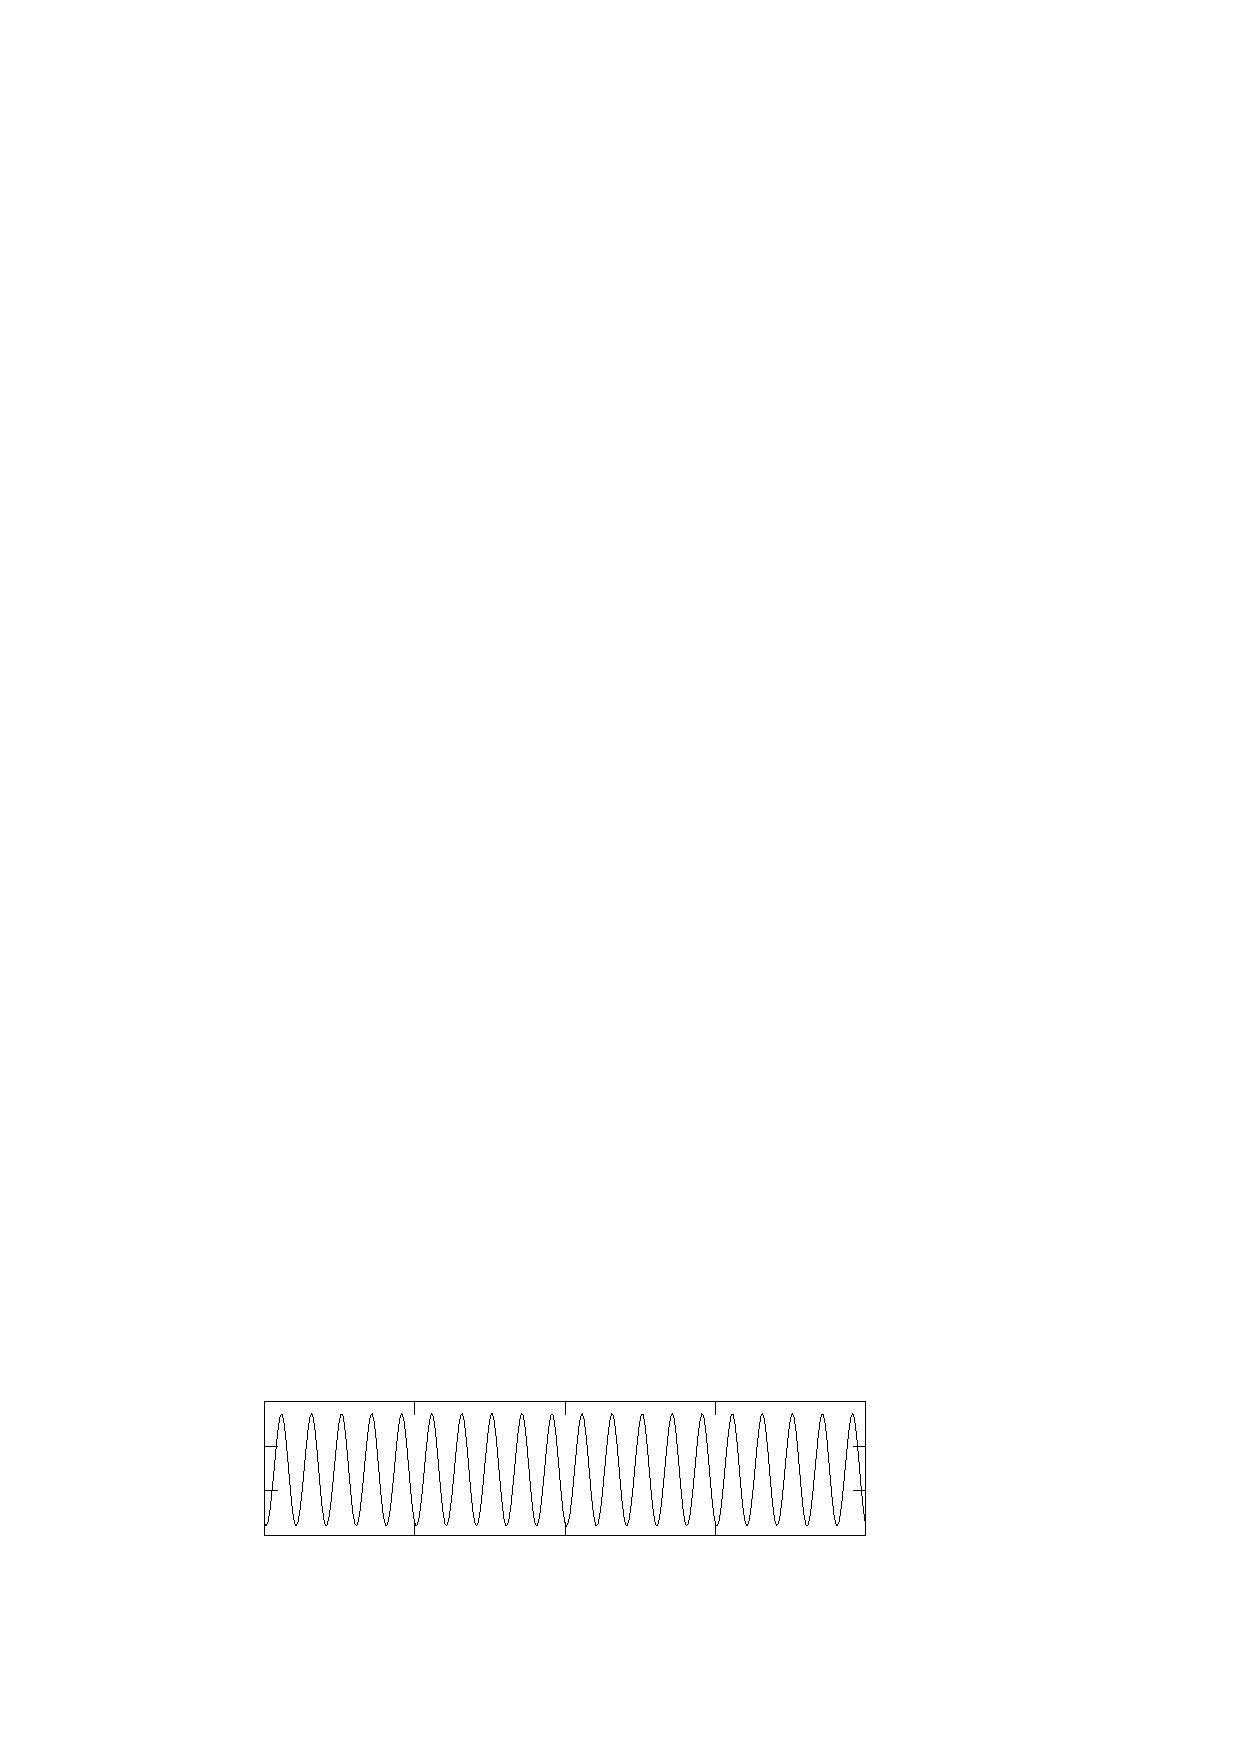
\includegraphics{flat-rho-30-Fo7_821e-02}%
%\end{picture}%
%\begingroup
%\setlength{\unitlength}{0.0200bp}%
%\begin{picture}(18000,5400)(0,0)%
%\put(2475,1650){\makebox(0,0)[r]{\strut{}1.400}}%
%\put(2475,2717){\makebox(0,0)[r]{\strut{}1.405}}%
%\put(2475,3783){\makebox(0,0)[r]{\strut{}1.410}}%
%\put(2475,4850){\makebox(0,0)[r]{\strut{}1.415}}%
%\put(2750,1100){\makebox(0,0){\strut{} 1000}}%
%\put(6356,1100){\makebox(0,0){\strut{} 1005}}%
%\put(9963,1100){\makebox(0,0){\strut{} 1010}}%
%\put(13569,1100){\makebox(0,0){\strut{} 1015}}%
%\put(17175,1100){\makebox(0,0){\strut{} 1020}}%
%\put(550,3250){\rotatebox{90}{\makebox(0,0){\strut{}$y^\ast$}}}%
%\put(9962,275){\makebox(0,0){\strut{}$t^\ast$}}%
%\put(600,1000){\rotatebox{0}{\makebox(0,0){\strut{}(b)}}}%
%\end{picture}%
%\endgroup
%\endinput

%%GNUPLOT: LaTeX picture with Postscript
%\begin{picture}(0,0)%
%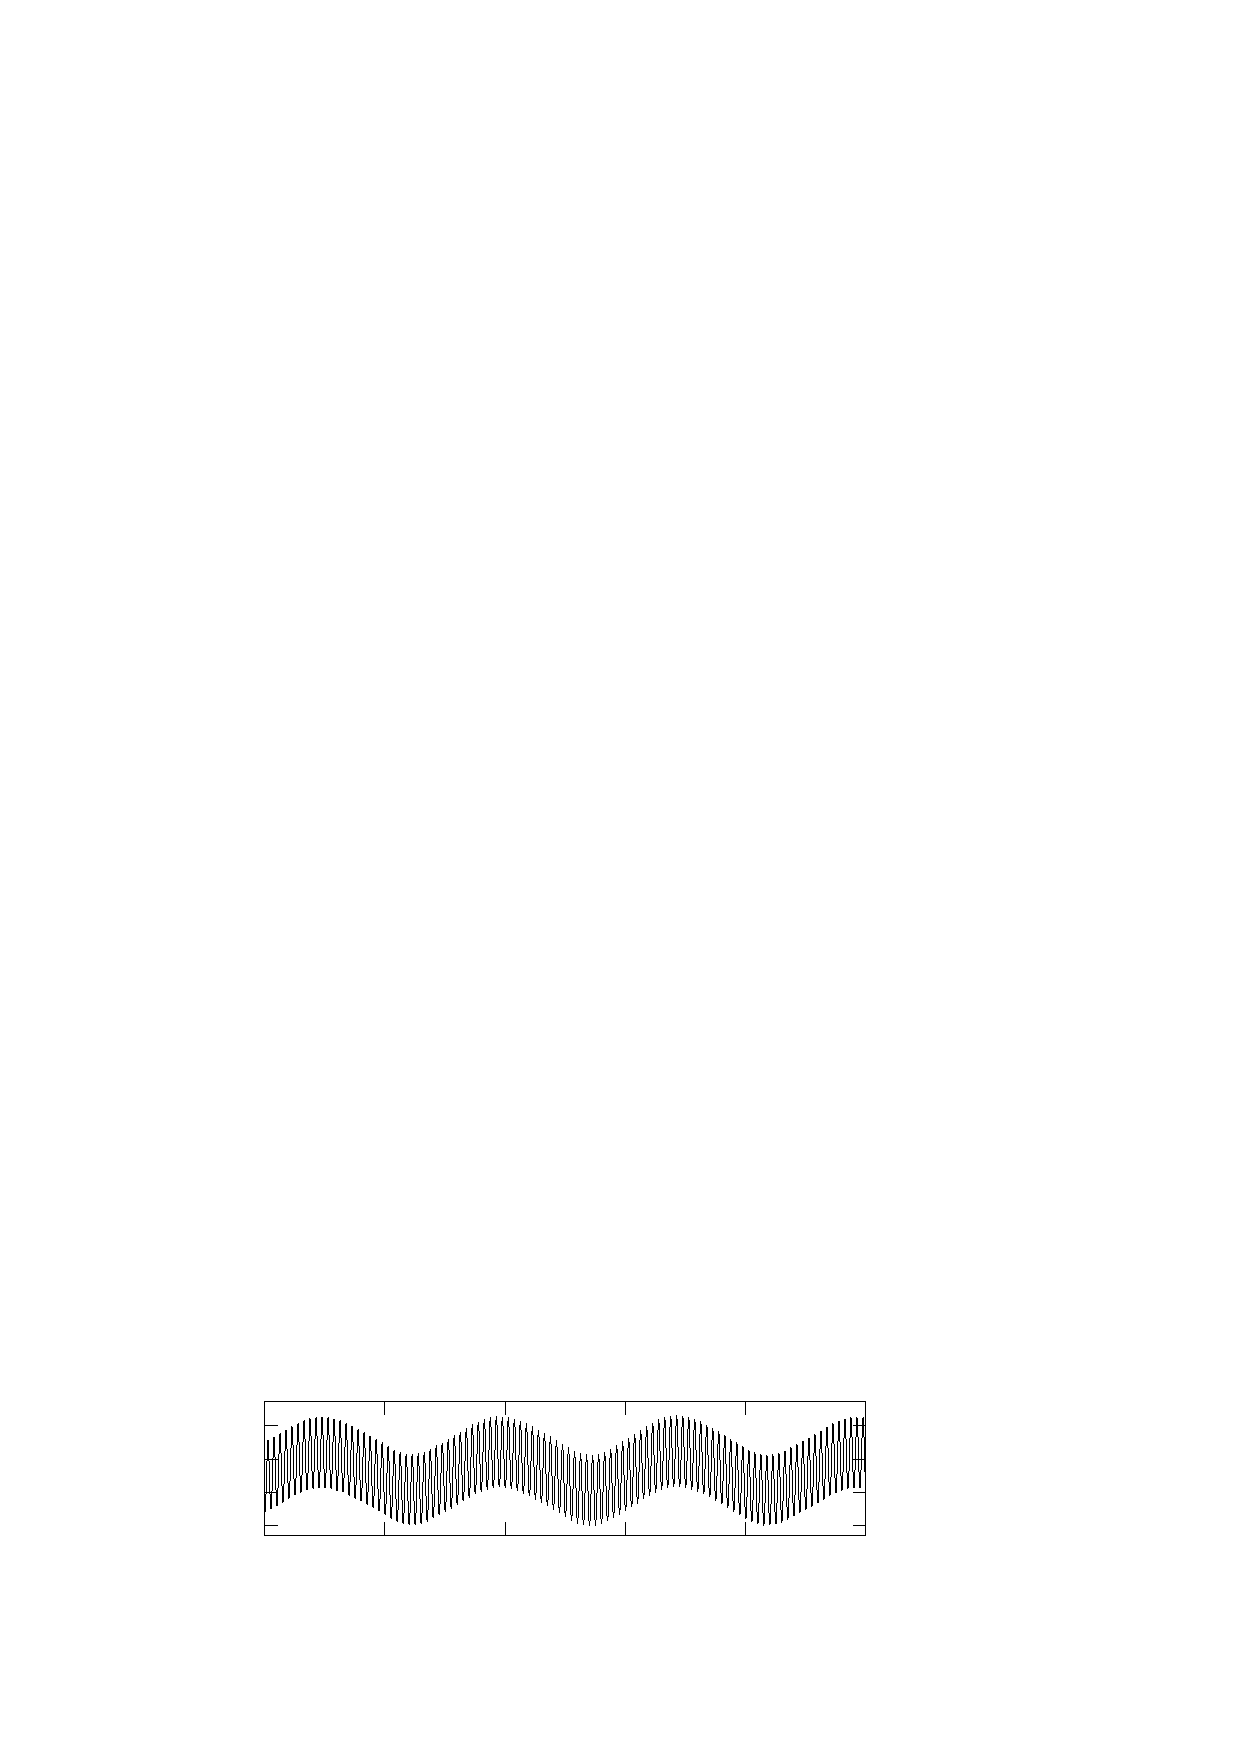
\includegraphics{flat-rho-30-Fo1_133e-01}%
%\end{picture}%
%\begingroup
%\setlength{\unitlength}{0.0200bp}%
%\begin{picture}(18000,5400)(0,0)%
%\put(2475,1879){\makebox(0,0)[r]{\strut{}1.488}}%
%\put(2475,2679){\makebox(0,0)[r]{\strut{}1.496}}%
%\put(2475,3479){\makebox(0,0)[r]{\strut{}1.505}}%
%\put(2475,4279){\makebox(0,0)[r]{\strut{}1.514}}%
%\put(2750,1100){\makebox(0,0){\strut{} 600}}%
%\put(5635,1100){\makebox(0,0){\strut{} 620}}%
%\put(8520,1100){\makebox(0,0){\strut{} 640}}%
%\put(11405,1100){\makebox(0,0){\strut{} 660}}%
%\put(14290,1100){\makebox(0,0){\strut{} 680}}%
%\put(17175,1100){\makebox(0,0){\strut{} 700}}%
%\put(550,3250){\rotatebox{90}{\makebox(0,0){\strut{}$y^\ast$}}}%
%\put(9962,275){\makebox(0,0){\strut{}$t^\ast$}}%
%\put(600,1000){\rotatebox{0}{\makebox(0,0){\strut{}(c)}}}%
%\end{picture}%
%\endgroup
%\endinput

%%GNUPLOT: LaTeX picture with Postscript
\begin{picture}(0,0)%
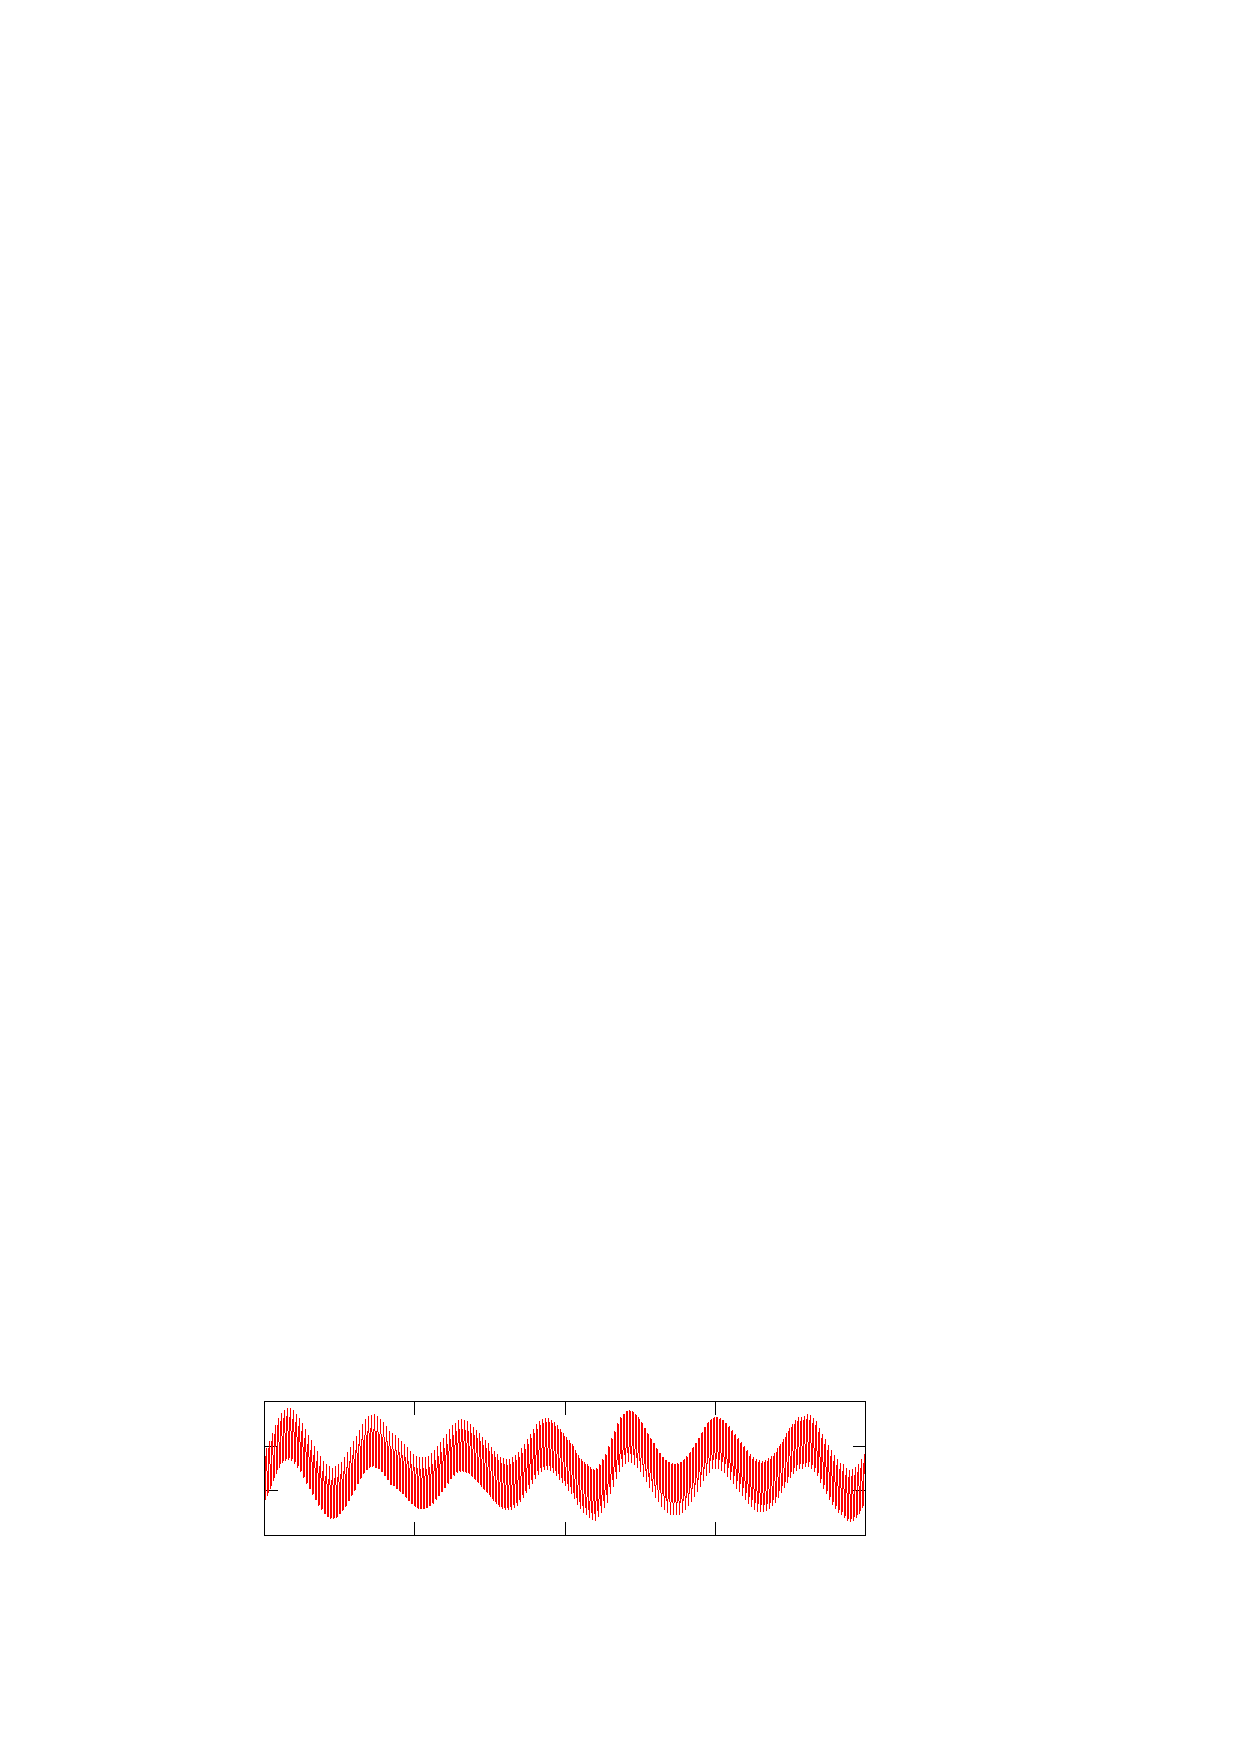
\includegraphics{flat-rho-30-Fo1_420e-01}%
\end{picture}%
\begingroup
\setlength{\unitlength}{0.0200bp}%
\begin{picture}(18000,5400)(0,0)%
\put(2475,1650){\makebox(0,0)[r]{\strut{}1.500}}%
\put(2475,2717){\makebox(0,0)[r]{\strut{}1.520}}%
\put(2475,3783){\makebox(0,0)[r]{\strut{}1.540}}%
\put(2475,4850){\makebox(0,0)[r]{\strut{}1.560}}%
\put(2750,1100){\makebox(0,0){\strut{} 1200}}%
\put(6356,1100){\makebox(0,0){\strut{} 1250}}%
\put(9963,1100){\makebox(0,0){\strut{} 1300}}%
\put(13569,1100){\makebox(0,0){\strut{} 1350}}%
\put(17175,1100){\makebox(0,0){\strut{} 1400}}%
\put(550,3250){\rotatebox{90}{\makebox(0,0){\strut{}$y^\ast$}}}%
\put(9962,275){\makebox(0,0){\strut{}$t^\ast$}}%
\put(600,2550){\rotatebox{90}{\makebox(0,0){\strut{}(d)}}}%
\end{picture}%
\endgroup
\endinput

%%GNUPLOT: LaTeX picture with Postscript
\begin{picture}(0,0)%
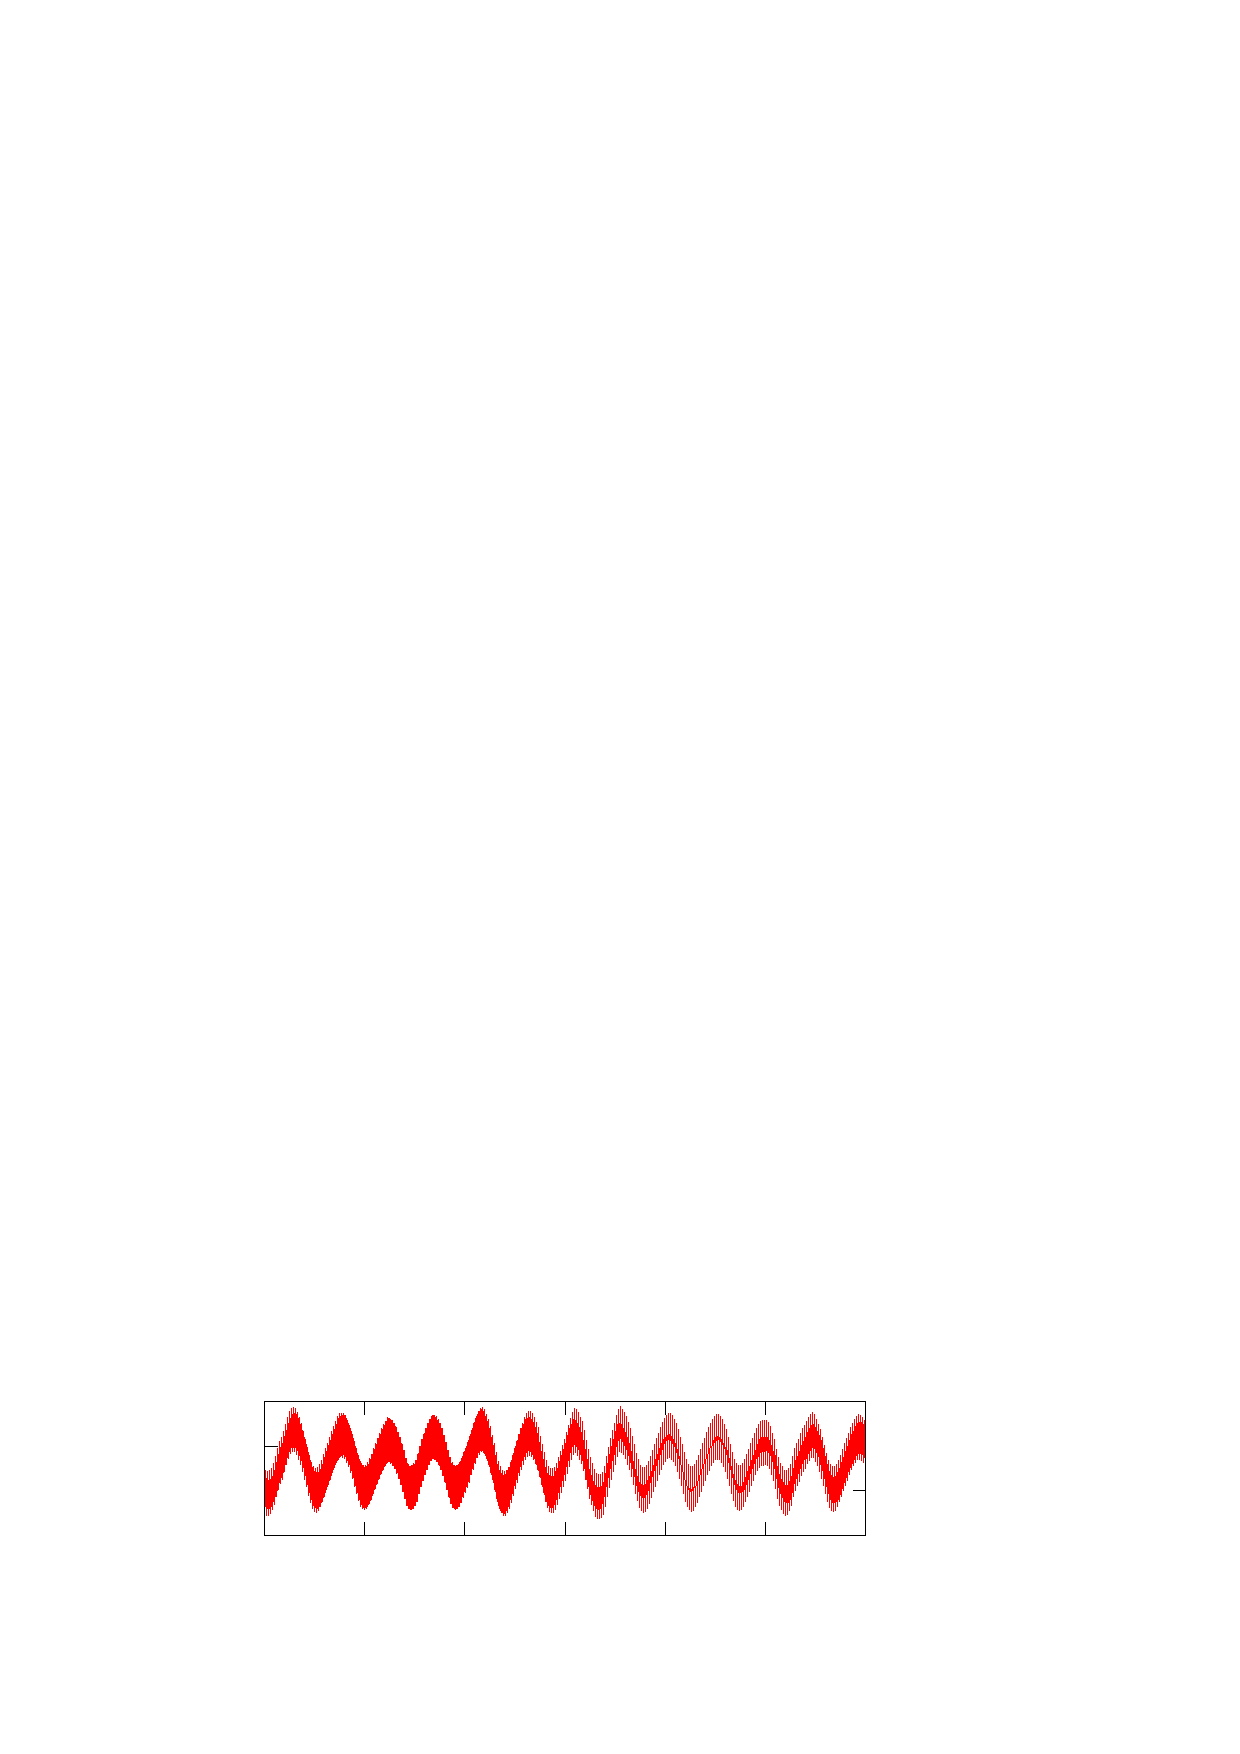
\includegraphics{flat-rho-30-Fo1_852e-01}%
\end{picture}%
\begingroup
\setlength{\unitlength}{0.0200bp}%
\begin{picture}(18000,5400)(0,0)%
\put(2475,1650){\makebox(0,0)[r]{\strut{}1.500}}%
\put(2475,2717){\makebox(0,0)[r]{\strut{}1.530}}%
\put(2475,3783){\makebox(0,0)[r]{\strut{}1.560}}%
\put(2475,4850){\makebox(0,0)[r]{\strut{}1.590}}%
\put(2750,1100){\makebox(0,0){\strut{} 1000}}%
\put(5154,1100){\makebox(0,0){\strut{} 1050}}%
\put(7558,1100){\makebox(0,0){\strut{} 1100}}%
\put(9963,1100){\makebox(0,0){\strut{} 1150}}%
\put(12367,1100){\makebox(0,0){\strut{} 1200}}%
\put(14771,1100){\makebox(0,0){\strut{} 1250}}%
\put(17175,1100){\makebox(0,0){\strut{} 1300}}%
\put(550,3250){\rotatebox{90}{\makebox(0,0){\strut{}$y^\ast$}}}%
\put(9962,275){\makebox(0,0){\strut{}$t^\ast$}}%
\put(600,2550){\rotatebox{90}{\makebox(0,0){\strut{}(e)}}}%
\end{picture}%
\endgroup
\endinput

\caption{\label{fig:paths-rho-30-flat}
Trayectoria vertical de la part'icula s'olida $\rho_p/\rho_f=50$ sobre el tiempo en la cavidad plana para
(a) $P_o^\ast = 4.45\times 10^{-3} $, (b) $P_o^\ast = 6.25\times 10^{-3}$ y (c) $P_o^\ast = 9.05\times 10^{-3}$.
%(d) $P_o^\ast = 1.135\times 10^{-2}$ y (e) $P_o^\ast = 1.48\times 10^{-2}$.
}
\end{figure}
\begin{figure}
%\put(600,2550){\rotatebox{90}{\makebox(0,0){\strut{}(a)}}}%
%%GNUPLOT: LaTeX picture with Postscript
%\begin{picture}(0,0)%
%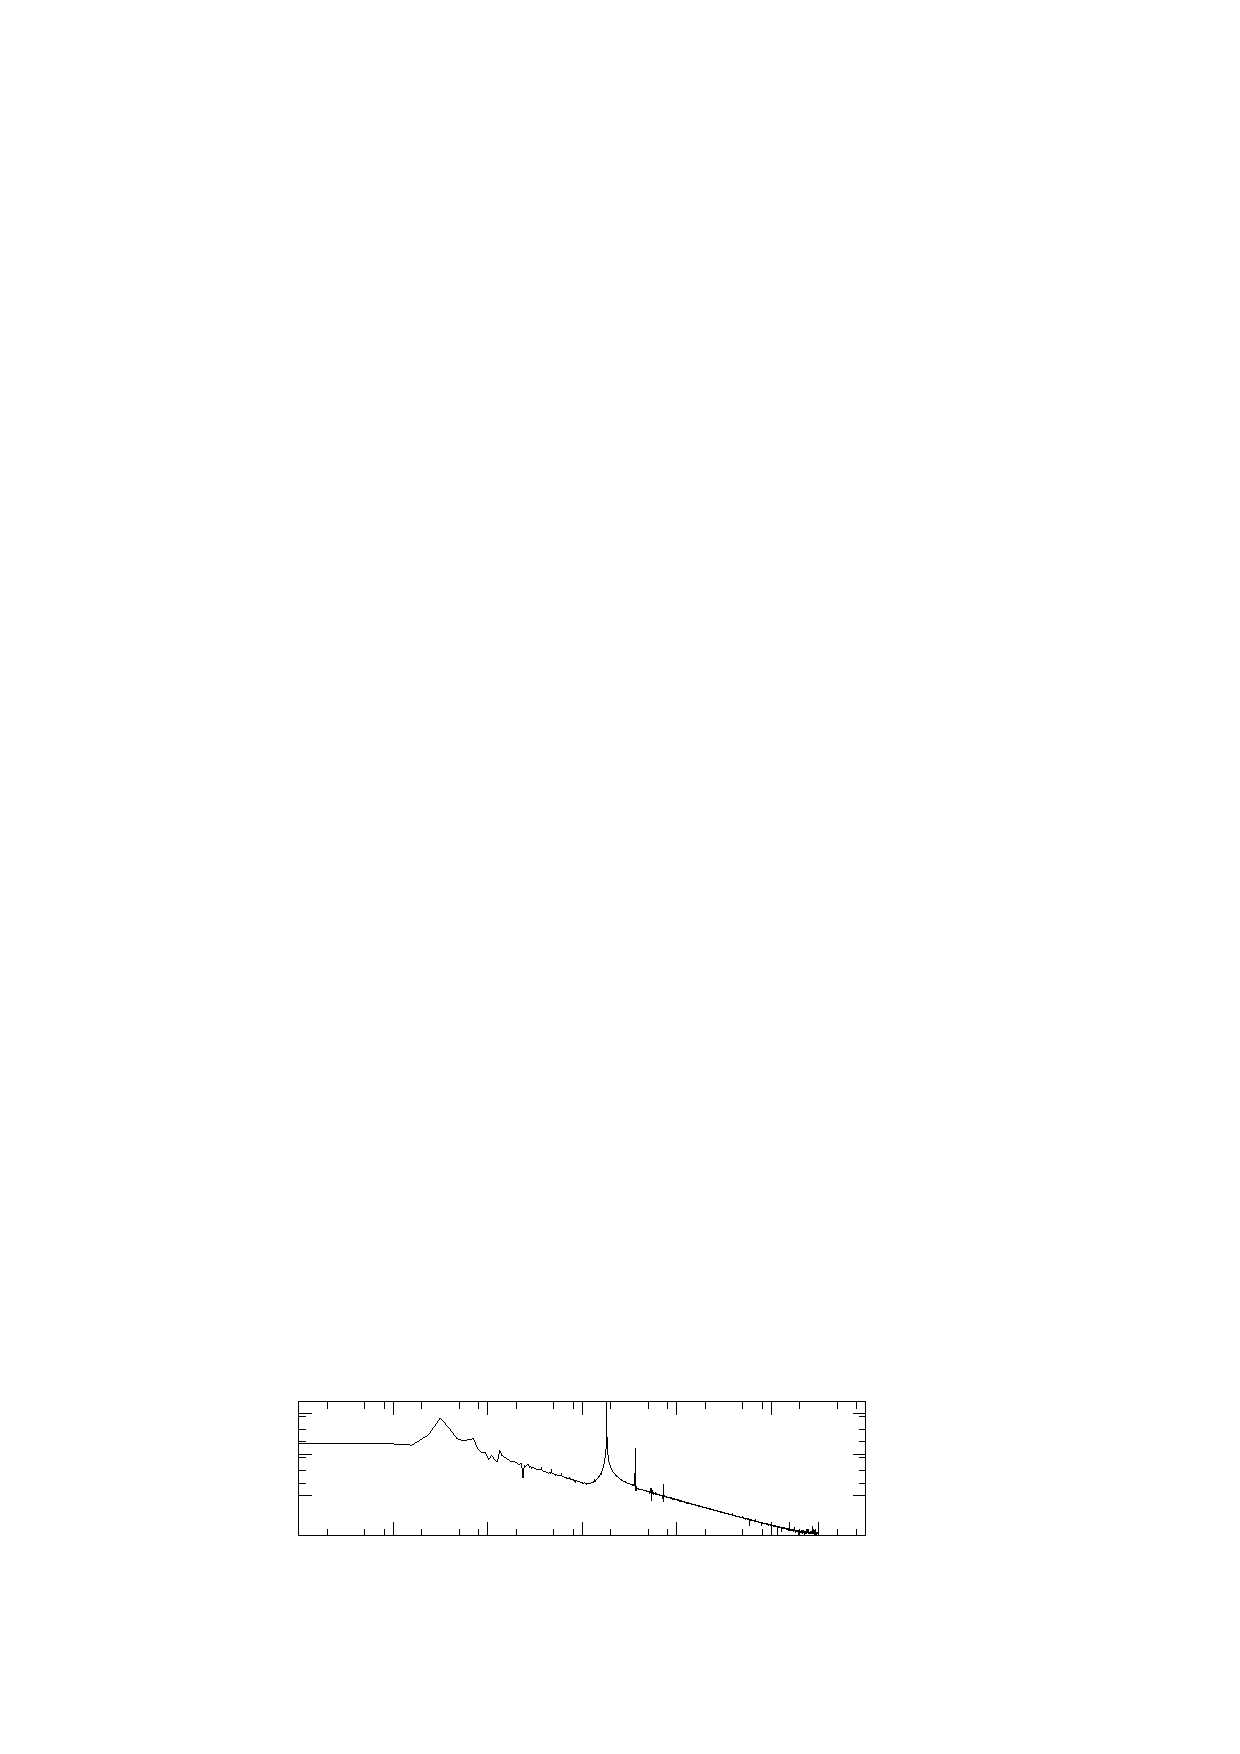
\includegraphics{flat-rho-30-Fo5_569e-02-spectrum}%
%\end{picture}%
%\begingroup
%\setlength{\unitlength}{0.0200bp}%
%\begin{picture}(18000,5400)(0,0)%
%\put(3300,2598){\makebox(0,0)[r]{\strut{}1.30e-13}}%
%\put(3300,3586){\makebox(0,0)[r]{\strut{}2.16e-10}}%
%\put(3300,4574){\makebox(0,0)[r]{\strut{}3.60e-07}}%
%\put(3575,1100){\makebox(0,0){\strut{} 1e-05}}%
%\put(5842,1100){\makebox(0,0){\strut{} 1e-04}}%
%\put(8108,1100){\makebox(0,0){\strut{} 0.001}}%
%\put(10375,1100){\makebox(0,0){\strut{} 0.01}}%
%\put(12642,1100){\makebox(0,0){\strut{} 0.1}}%
%\put(14908,1100){\makebox(0,0){\strut{} 1}}%
%\put(17175,1100){\makebox(0,0){\strut{} 10}}%
%\put(550,3250){\rotatebox{90}{\makebox(0,0){\strut{}$PSD$}}}%
%\put(10375,275){\makebox(0,0){\strut{}$\omega$}}%
%\put(600,1000){\makebox(0,0){\strut{}(a)}}%
%\end{picture}%
%\endgroup
%\endinput

%%GNUPLOT: LaTeX picture with Postscript
%\begin{picture}(0,0)%
%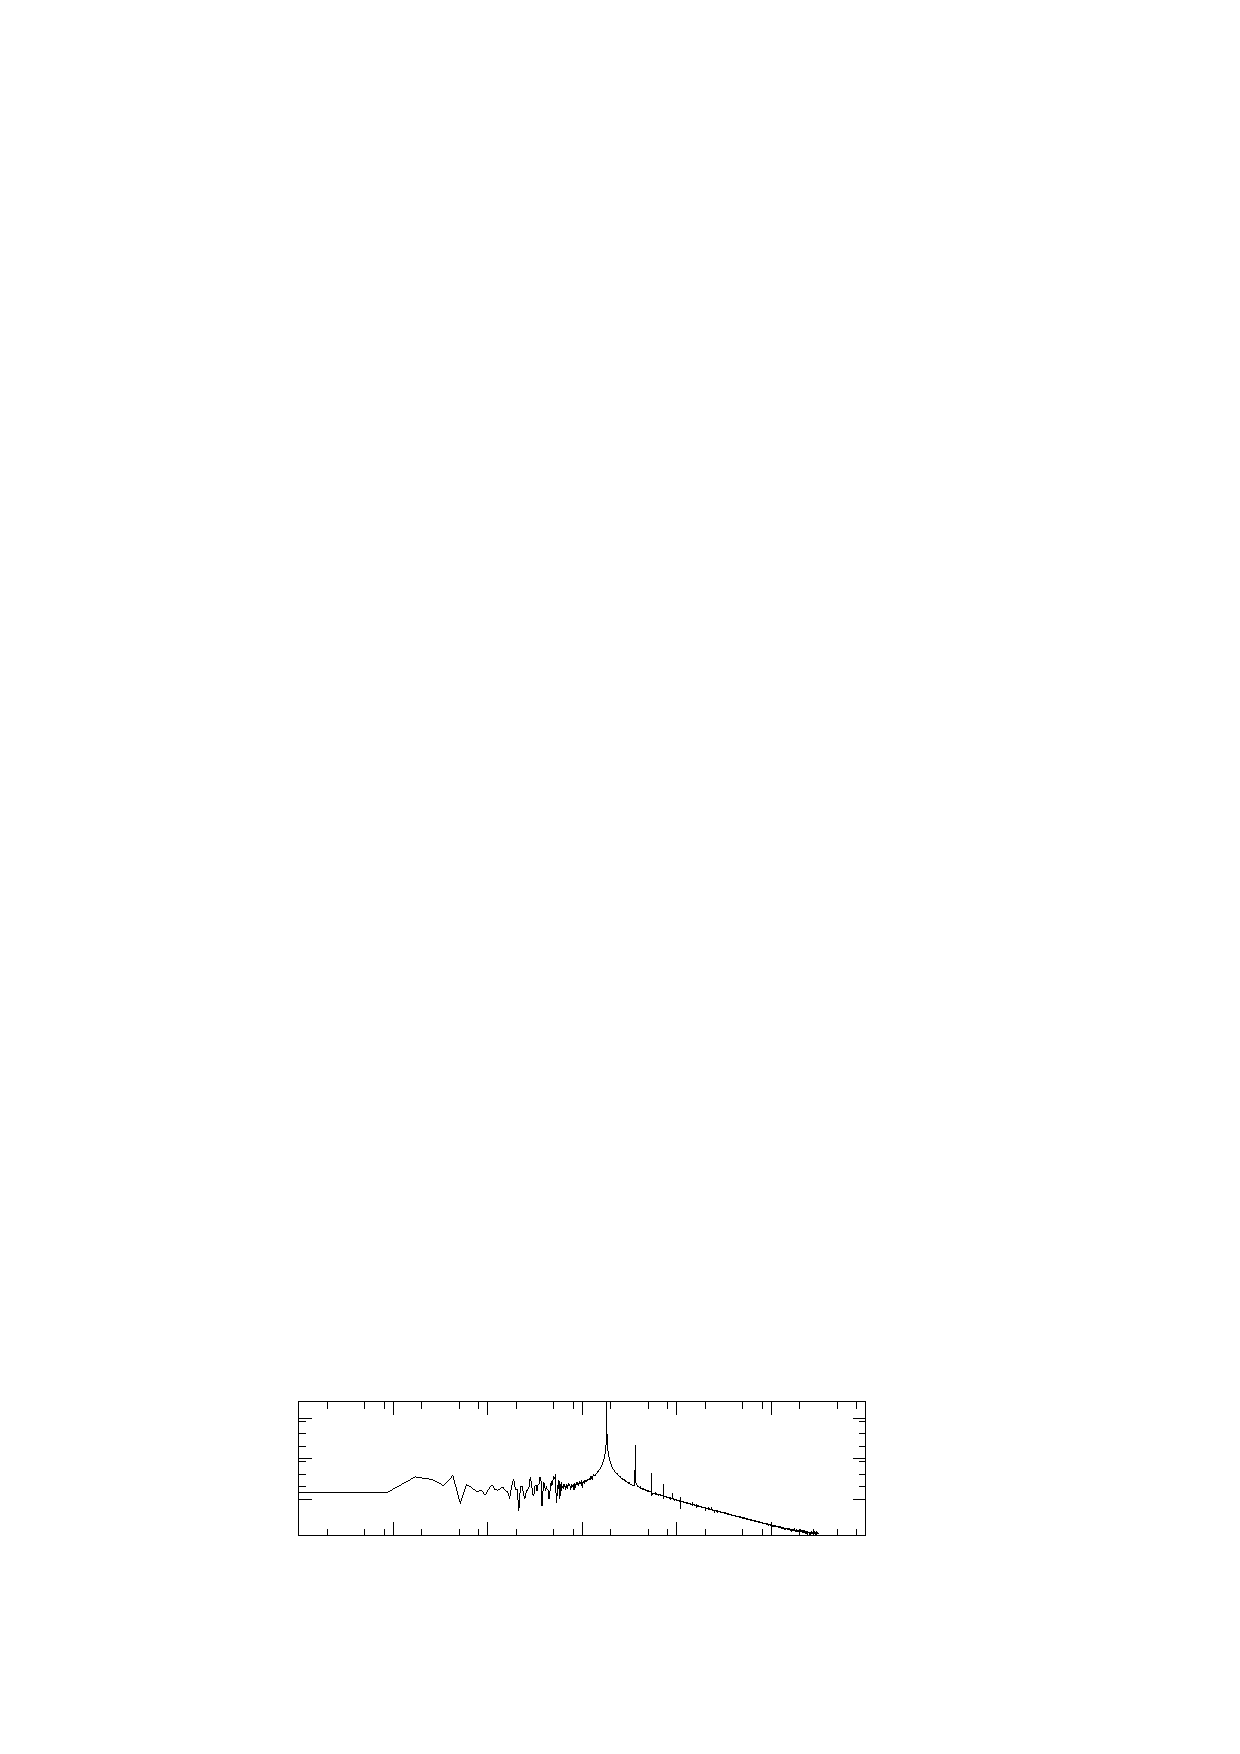
\includegraphics{flat-rho-30-Fo7_821e-02-spectrum}%
%\end{picture}%
%\begingroup
%\setlength{\unitlength}{0.0200bp}%
%\begin{picture}(18000,5400)(0,0)%
%\put(3300,2512){\makebox(0,0)[r]{\strut{}1.30e-13}}%
%\put(3300,3484){\makebox(0,0)[r]{\strut{}2.16e-10}}%
%\put(3300,4456){\makebox(0,0)[r]{\strut{}3.60e-07}}%
%\put(3575,1100){\makebox(0,0){\strut{} 1e-05}}%
%\put(5842,1100){\makebox(0,0){\strut{} 1e-04}}%
%\put(8108,1100){\makebox(0,0){\strut{} 0.001}}%
%\put(10375,1100){\makebox(0,0){\strut{} 0.01}}%
%\put(12642,1100){\makebox(0,0){\strut{} 0.1}}%
%\put(14908,1100){\makebox(0,0){\strut{} 1}}%
%\put(17175,1100){\makebox(0,0){\strut{} 10}}%
%\put(550,3250){\rotatebox{90}{\makebox(0,0){\strut{}$PSD$}}}%
%\put(10375,275){\makebox(0,0){\strut{}$\omega$}}%
%\put(600,1000){\rotatebox{0}{\makebox(0,0){\strut{}(b)}}}%
%\end{picture}%
%\endgroup
%\endinput

%%GNUPLOT: LaTeX picture with Postscript
%\begin{picture}(0,0)%
%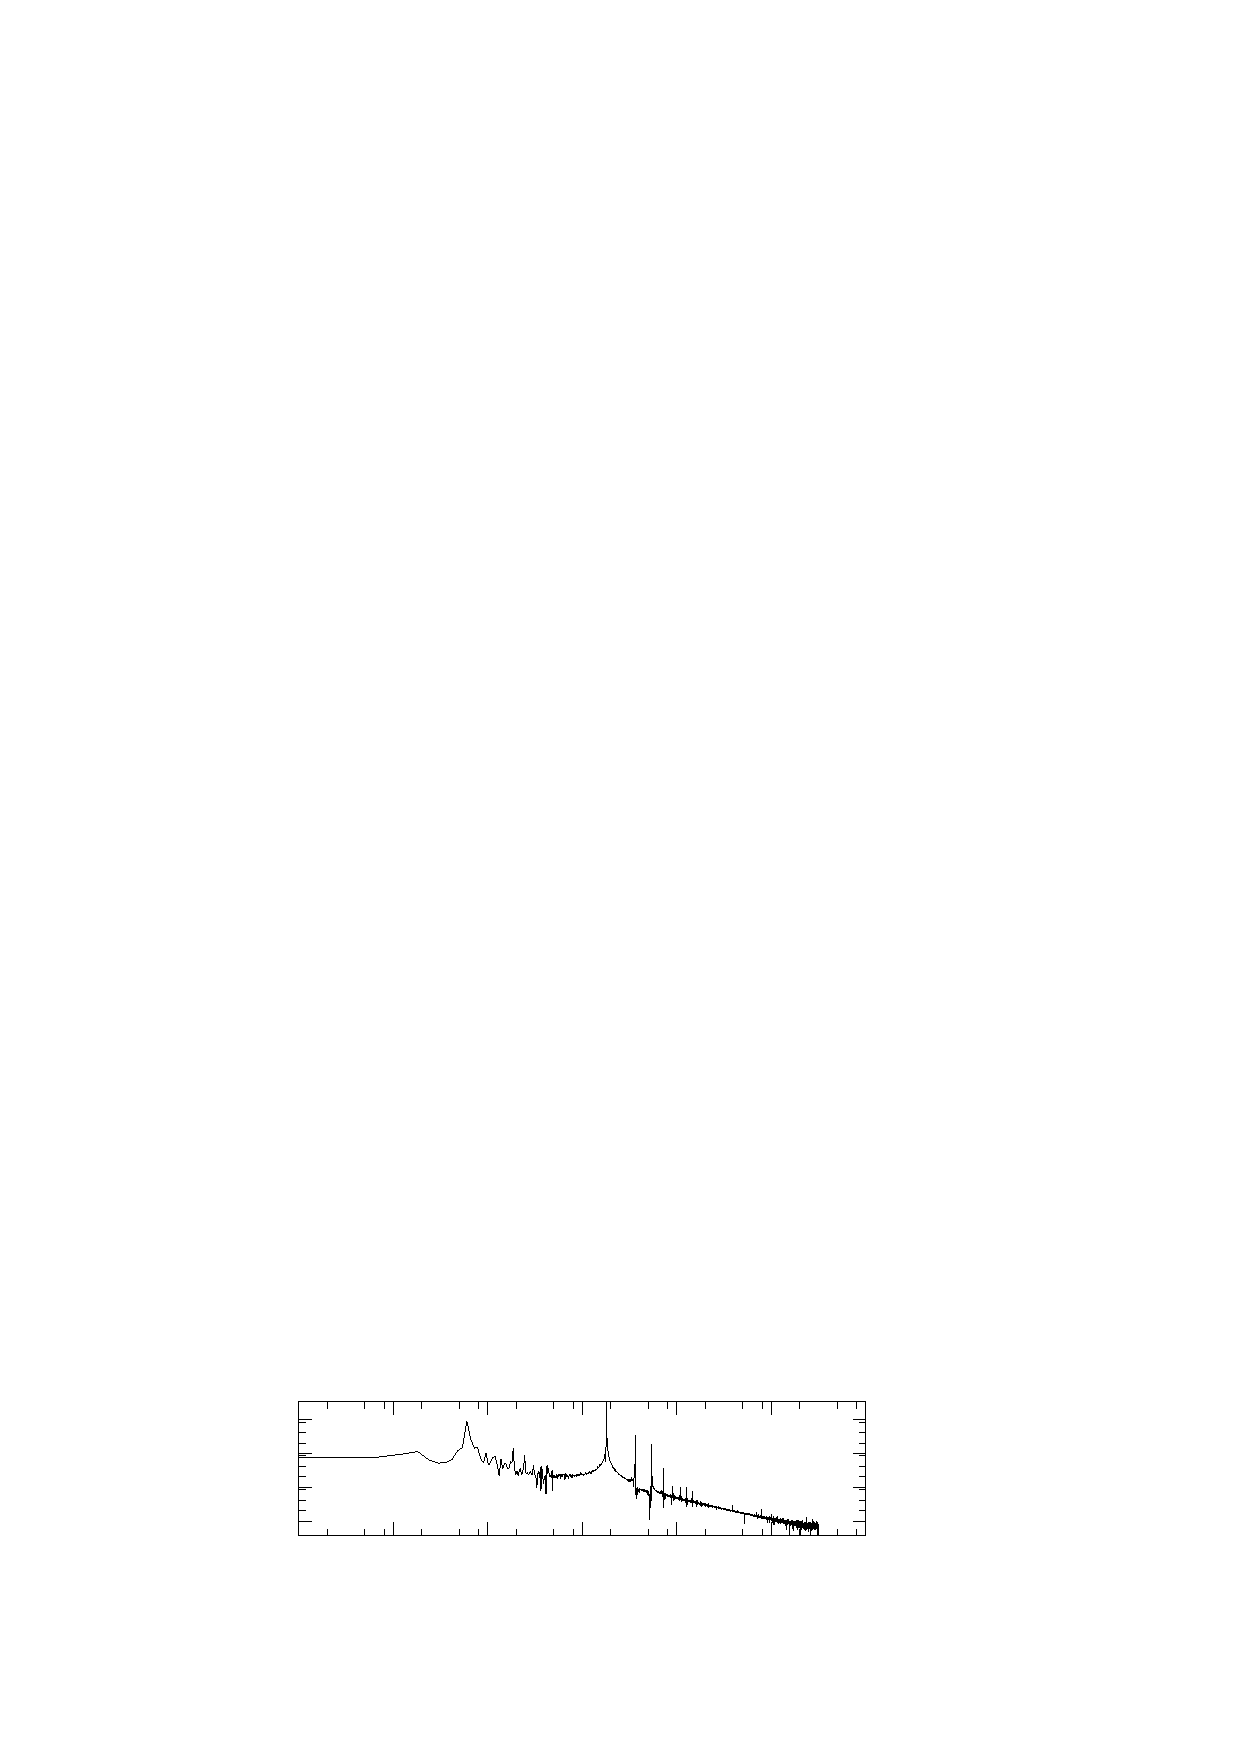
\includegraphics{flat-rho-30-Fo1_133e-01-spectrum}%
%\end{picture}%
%\begingroup
%\setlength{\unitlength}{0.0200bp}%
%\begin{picture}(18000,5400)(0,0)%
%\put(3300,1987){\makebox(0,0)[r]{\strut{}7.78e-17}}%
%\put(3300,2798){\makebox(0,0)[r]{\strut{}1.30e-13}}%
%\put(3300,3609){\makebox(0,0)[r]{\strut{}2.16e-10}}%
%\put(3300,4420){\makebox(0,0)[r]{\strut{}3.60e-07}}%
%\put(3575,1100){\makebox(0,0){\strut{} 1e-05}}%
%\put(5842,1100){\makebox(0,0){\strut{} 1e-04}}%
%\put(8108,1100){\makebox(0,0){\strut{} 0.001}}%
%\put(10375,1100){\makebox(0,0){\strut{} 0.01}}%
%\put(12642,1100){\makebox(0,0){\strut{} 0.1}}%
%\put(14908,1100){\makebox(0,0){\strut{} 1}}%
%\put(17175,1100){\makebox(0,0){\strut{} 10}}%
%\put(550,3250){\rotatebox{90}{\makebox(0,0){\strut{}$PSD$}}}%
%\put(10375,275){\makebox(0,0){\strut{}$\omega$}}%
%\put(600,1000){\rotatebox{0}{\makebox(0,0){\strut{}(c)}}}%
%\end{picture}%
%\endgroup
%\endinput

%%GNUPLOT: LaTeX picture with Postscript
\begin{picture}(0,0)%
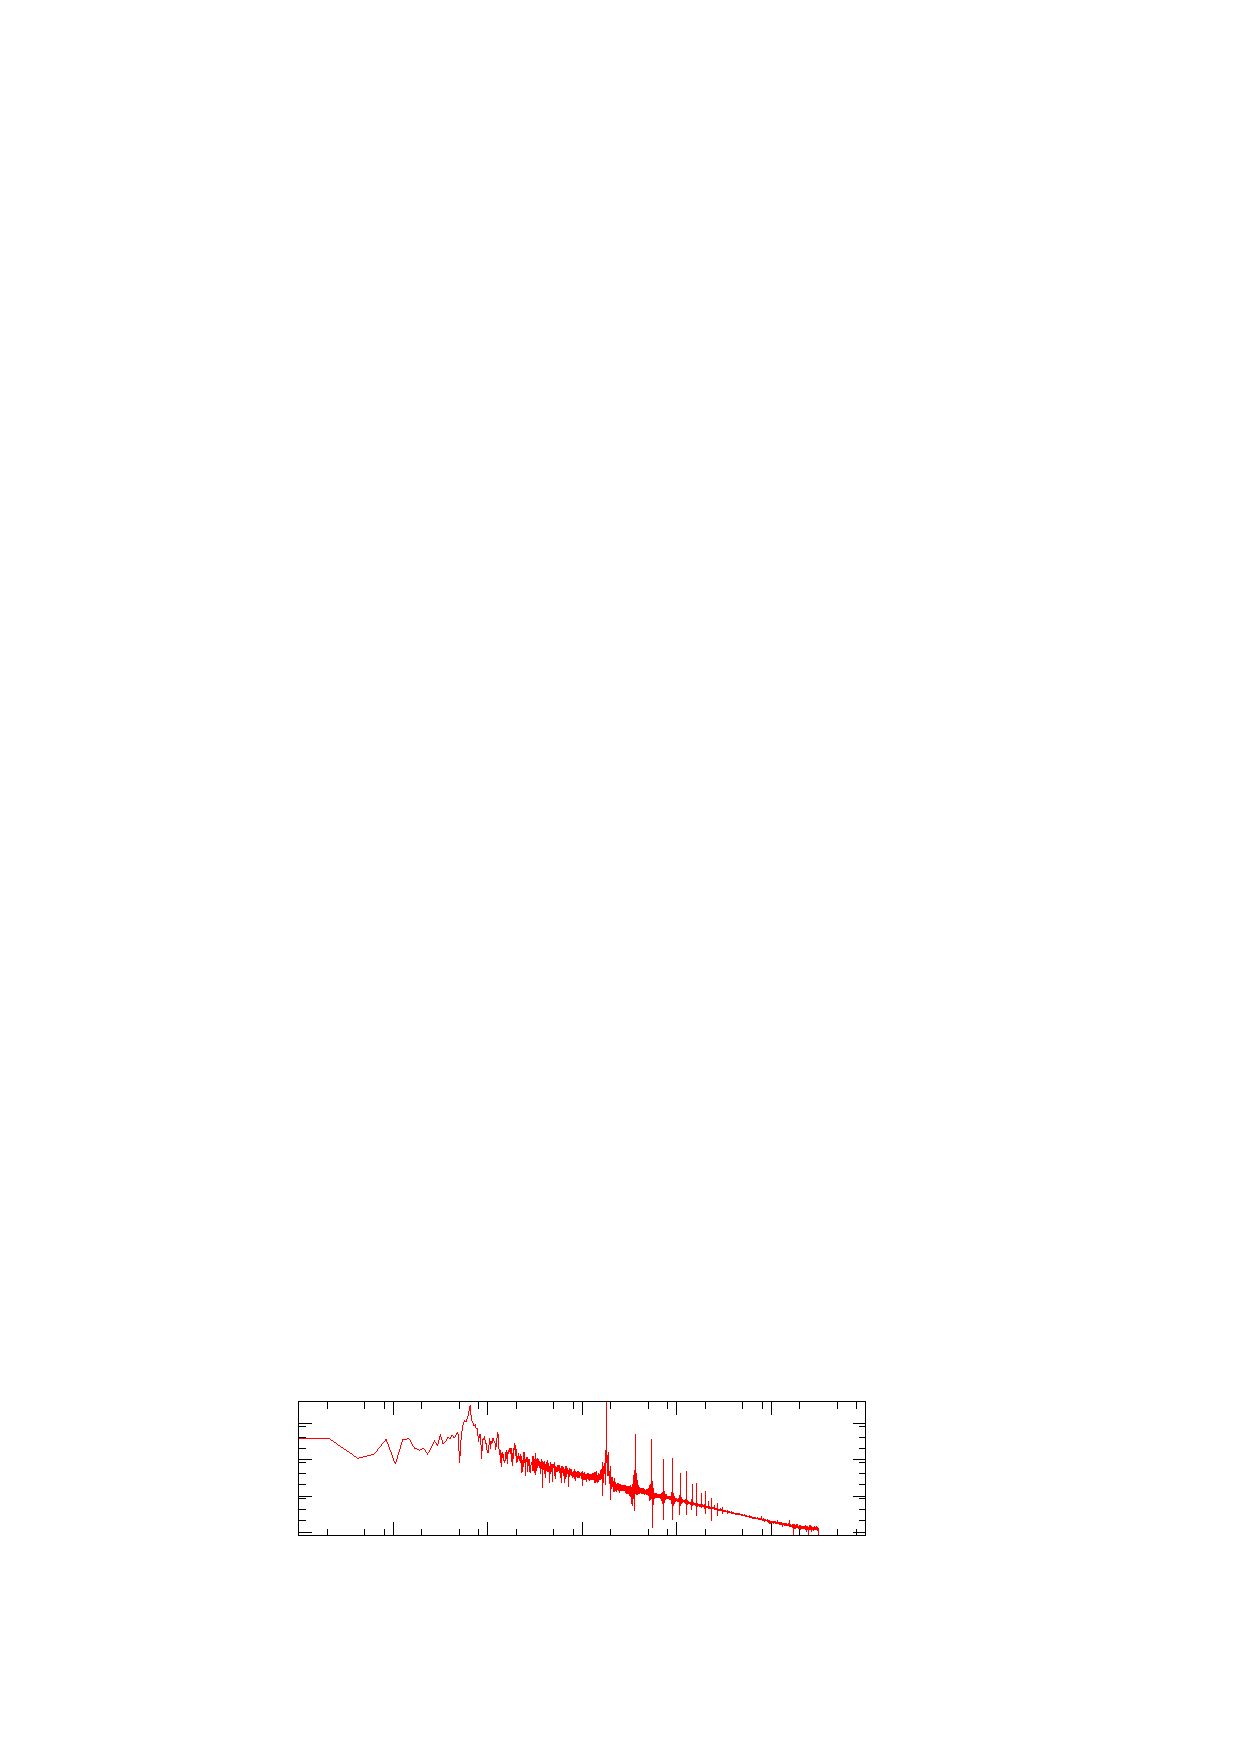
\includegraphics{flat-rho-30-Fo1_420e-01-spectrum}%
\end{picture}%
\begingroup
\setlength{\unitlength}{0.0200bp}%
\begin{picture}(18000,5400)(0,0)%
\put(3300,1724){\makebox(0,0)[r]{\strut{}7.78e-17}}%
\put(3300,2591){\makebox(0,0)[r]{\strut{}1.30e-13}}%
\put(3300,3457){\makebox(0,0)[r]{\strut{}2.16e-10}}%
\put(3300,4324){\makebox(0,0)[r]{\strut{}3.60e-07}}%
\put(3575,1100){\makebox(0,0){\strut{} 1e-05}}%
\put(5842,1100){\makebox(0,0){\strut{} 0.0001}}%
\put(8108,1100){\makebox(0,0){\strut{} 0.001}}%
\put(10375,1100){\makebox(0,0){\strut{} 0.01}}%
\put(12642,1100){\makebox(0,0){\strut{} 0.1}}%
\put(14908,1100){\makebox(0,0){\strut{} 1}}%
\put(17175,1100){\makebox(0,0){\strut{} 10}}%
\put(550,3250){\rotatebox{90}{\makebox(0,0){\strut{}$PSD$}}}%
\put(10375,275){\makebox(0,0){\strut{}$\omega$}}%
\put(600,2550){\rotatebox{90}{\makebox(0,0){\strut{}(d)}}}%
\end{picture}%
\endgroup
\endinput

%%GNUPLOT: LaTeX picture with Postscript
\begin{picture}(0,0)%
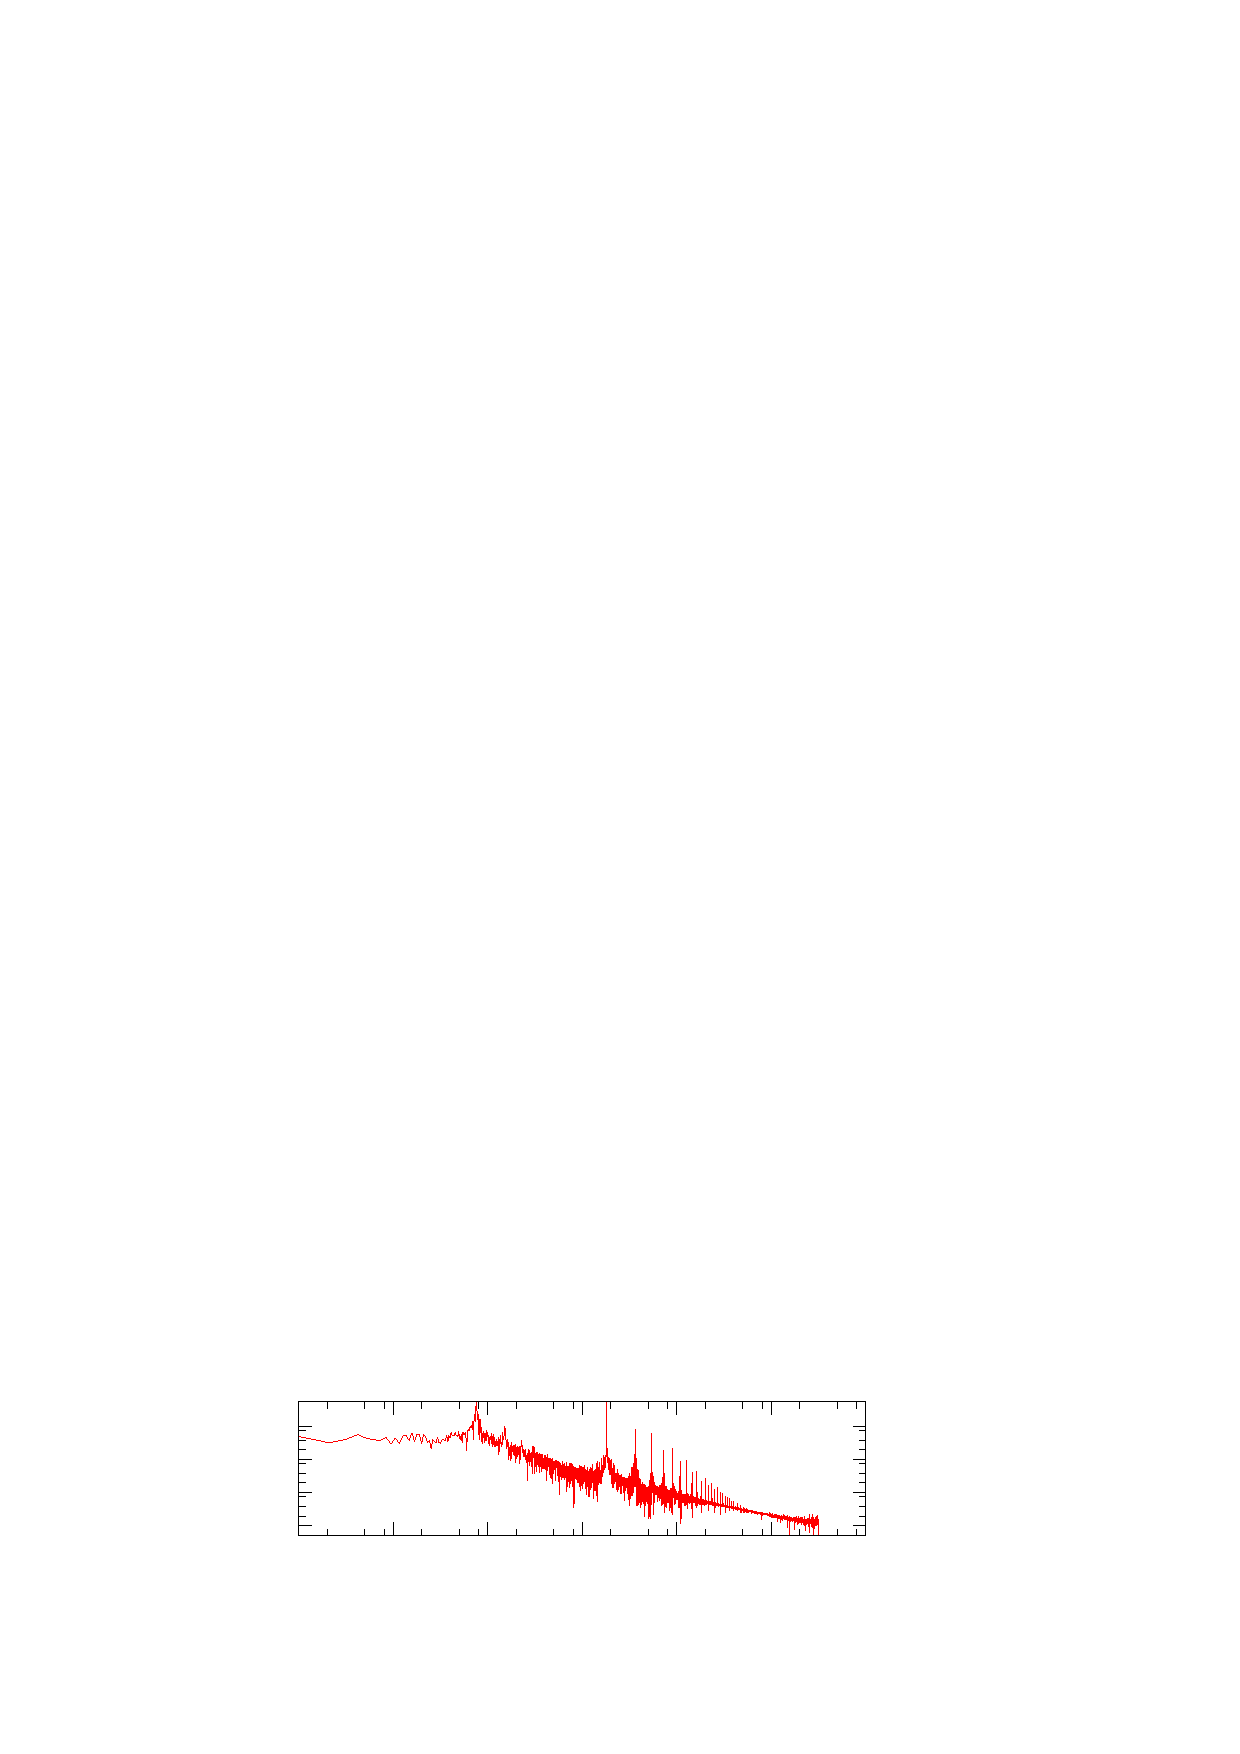
\includegraphics{flat-rho-30-Fo1_852e-01-spectrum}%
\end{picture}%
\begingroup
\setlength{\unitlength}{0.0200bp}%
\begin{picture}(18000,5400)(0,0)%
\put(3300,1878){\makebox(0,0)[r]{\strut{}1.02e-17}}%
\put(3300,2672){\makebox(0,0)[r]{\strut{}2.56e-14}}%
\put(3300,3466){\makebox(0,0)[r]{\strut{}6.40e-11}}%
\put(3300,4259){\makebox(0,0)[r]{\strut{}1.60e-07}}%
\put(3575,1100){\makebox(0,0){\strut{} 1e-05}}%
\put(5842,1100){\makebox(0,0){\strut{} 0.0001}}%
\put(8108,1100){\makebox(0,0){\strut{} 0.001}}%
\put(10375,1100){\makebox(0,0){\strut{} 0.01}}%
\put(12642,1100){\makebox(0,0){\strut{} 0.1}}%
\put(14908,1100){\makebox(0,0){\strut{} 1}}%
\put(17175,1100){\makebox(0,0){\strut{} 10}}%
\put(550,3250){\rotatebox{90}{\makebox(0,0){\strut{}$PSD$}}}%
\put(10375,275){\makebox(0,0){\strut{}$\omega$}}%
\put(600,2550){\rotatebox{90}{\makebox(0,0){\strut{}(e)}}}%
\end{picture}%
\endgroup
\endinput

\caption{\label{fig:paths-rho-30-flat-spectrum}
Espectro de potencia del movimiento vertical de la part'icula s'olida $\rho_p/\rho_f=50$ sobre el tiempo en la cavidad plana para
(a) $P_o^\ast = 4.45\times 10^{-3} $, (b) $P_o^\ast = 6.25\times 10^{-3}$ y (c) $P_o^\ast = 9.05\times 10^{-3}$. 
% (d) $P_o^\ast = 1.135\times 10^{-2}$ y (e) $P_o^\ast = 1.48\times 10^{-2}$.  
Los espectros de potencia corresponden a las trayectorias mostradas en las 
figuras~\ref{fig:paths-rho-30-flat} (b), (b) y (c).
}
\end{figure}

En las figuras~\ref{fig:paths-rho-30-flat} (a), (b) y (c) se muestra la trayectoria de la part'icula
s'olida en la cavidad plana para $P_o^\ast = 4.45\times 10^{-3} $, $P_o^\ast = 6.25\times 10^{-3}$ y $P_o^\ast = 9.05\times 10^{-3}$,
respectivamente. Al aumentar la cantidad de movimiento agregada, adem'as de aumentar la amplitud de la oscilaci'on
de la part'icula, tambien puede pasar por reg'imenes de oscilaci'on con una frecuencia o dos, como ha venido sucediendo
en las simulaciones num'ericas previas. 
En las figuras~\ref{fig:paths-rho-30-flat-spectrum} (a), (b) y (c) se muestran los espectros
de potencia para las trayectorias mostradas y se puede observar que  la presencia de arm'onicos de la frecuencia
de la fuente ac'ustica  ya es una constante.



\begin{figure}
%\put(600,2550){\rotatebox{90}{\makebox(0,0){\strut{}(a)}}}%
%GNUPLOT: LaTeX picture with Postscript
\begin{picture}(0,0)%
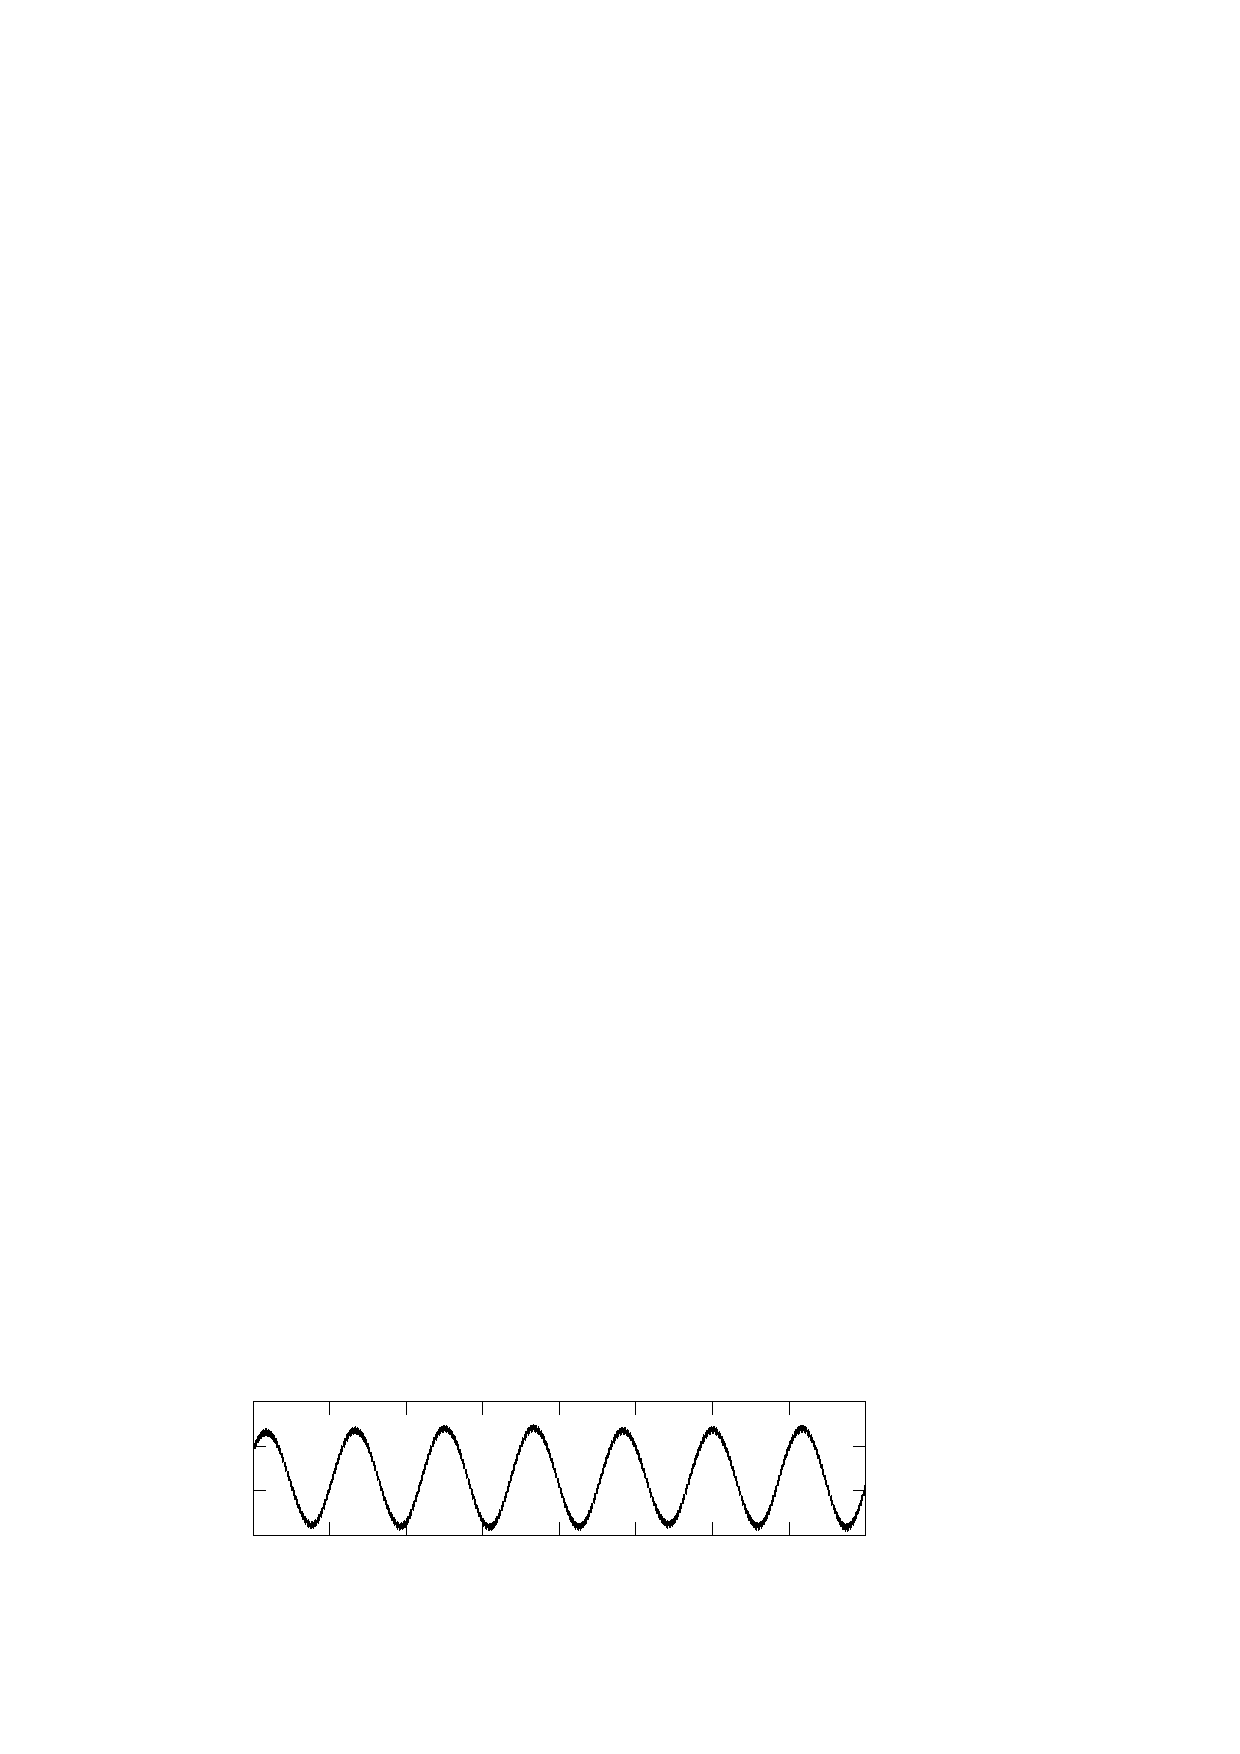
\includegraphics{rounded-rhop30-Fo7_508e-03}%
\end{picture}%
\begingroup
\setlength{\unitlength}{0.0200bp}%
\begin{picture}(18000,5400)(0,0)%
\put(2200,1650){\makebox(0,0)[r]{\strut{}1.14}}%
\put(2200,2717){\makebox(0,0)[r]{\strut{}1.20}}%
\put(2200,3783){\makebox(0,0)[r]{\strut{}1.26}}%
\put(2200,4850){\makebox(0,0)[r]{\strut{}1.32}}%
\put(2475,1100){\makebox(0,0){\strut{} 1800}}%
\put(6150,1100){\makebox(0,0){\strut{} 1850}}%
\put(9825,1100){\makebox(0,0){\strut{} 1900}}%
\put(13500,1100){\makebox(0,0){\strut{} 1950}}%
\put(17175,1100){\makebox(0,0){\strut{} 2000}}%
\put(550,3250){\rotatebox{90}{\makebox(0,0){\strut{}$y^\ast$}}}%
\put(9825,275){\makebox(0,0){\strut{}$t^\ast$}}%
\put(600,1000){\rotatebox{0}{\makebox(0,0){\strut{}(a)}}}%
\end{picture}%
\endgroup
\endinput

%%GNUPLOT: LaTeX picture with Postscript
\begin{picture}(0,0)%
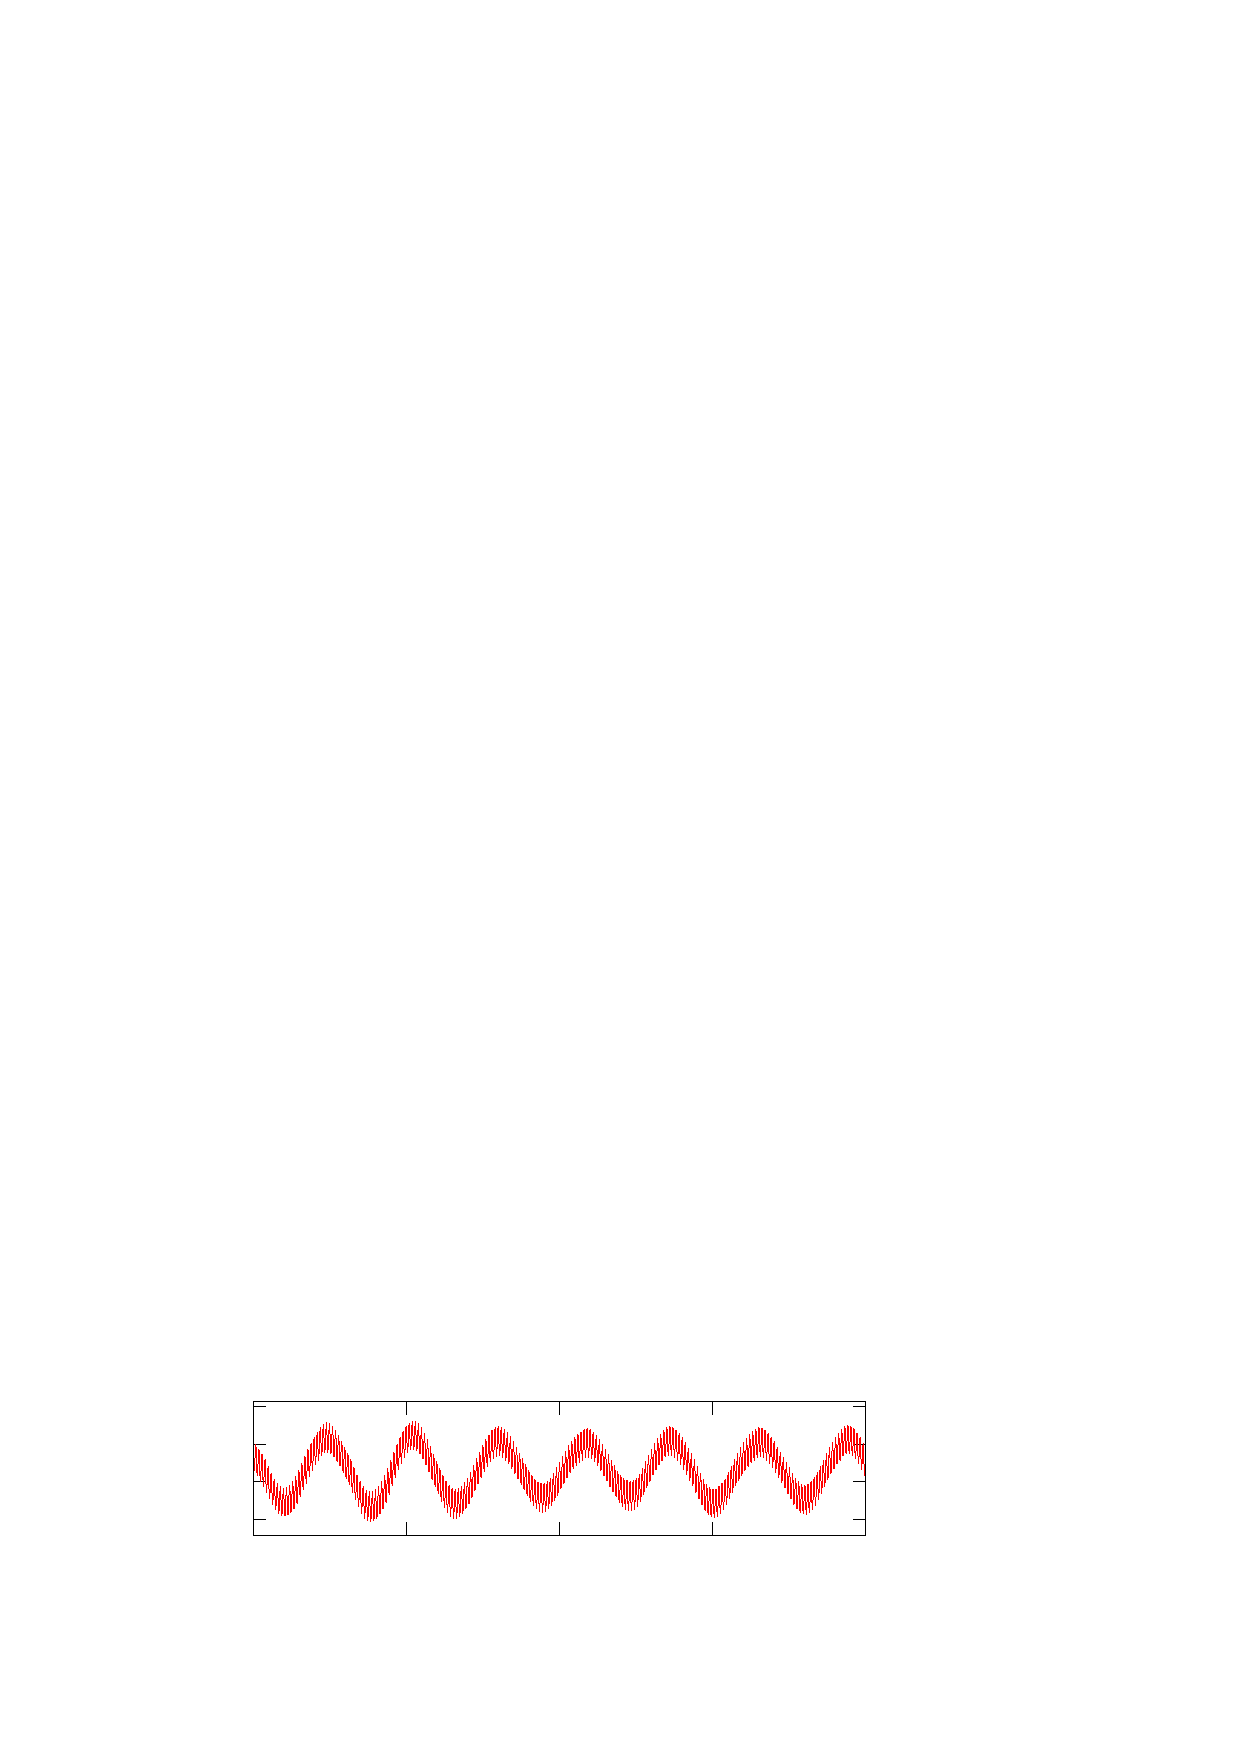
\includegraphics{rounded-rhop30-Fo3_191e-02}%
\end{picture}%
\begingroup
\setlength{\unitlength}{0.0200bp}%
\begin{picture}(18000,5400)(0,0)%
\put(2200,2036){\makebox(0,0)[r]{\strut{}1.41}}%
\put(2200,2935){\makebox(0,0)[r]{\strut{}1.44}}%
\put(2200,3834){\makebox(0,0)[r]{\strut{}1.47}}%
\put(2200,4732){\makebox(0,0)[r]{\strut{}1.50}}%
\put(2475,1100){\makebox(0,0){\strut{} 1600}}%
\put(6150,1100){\makebox(0,0){\strut{} 1650}}%
\put(9825,1100){\makebox(0,0){\strut{} 1700}}%
\put(13500,1100){\makebox(0,0){\strut{} 1750}}%
\put(17175,1100){\makebox(0,0){\strut{} 1800}}%
\put(550,3250){\rotatebox{90}{\makebox(0,0){\strut{}$y^\ast$}}}%
\put(9825,275){\makebox(0,0){\strut{}$t^\ast$}}%
\put(600,2550){\rotatebox{90}{\makebox(0,0){\strut{}(b)}}}%
\end{picture}%
\endgroup
\endinput

%GNUPLOT: LaTeX picture with Postscript
\begin{picture}(0,0)%
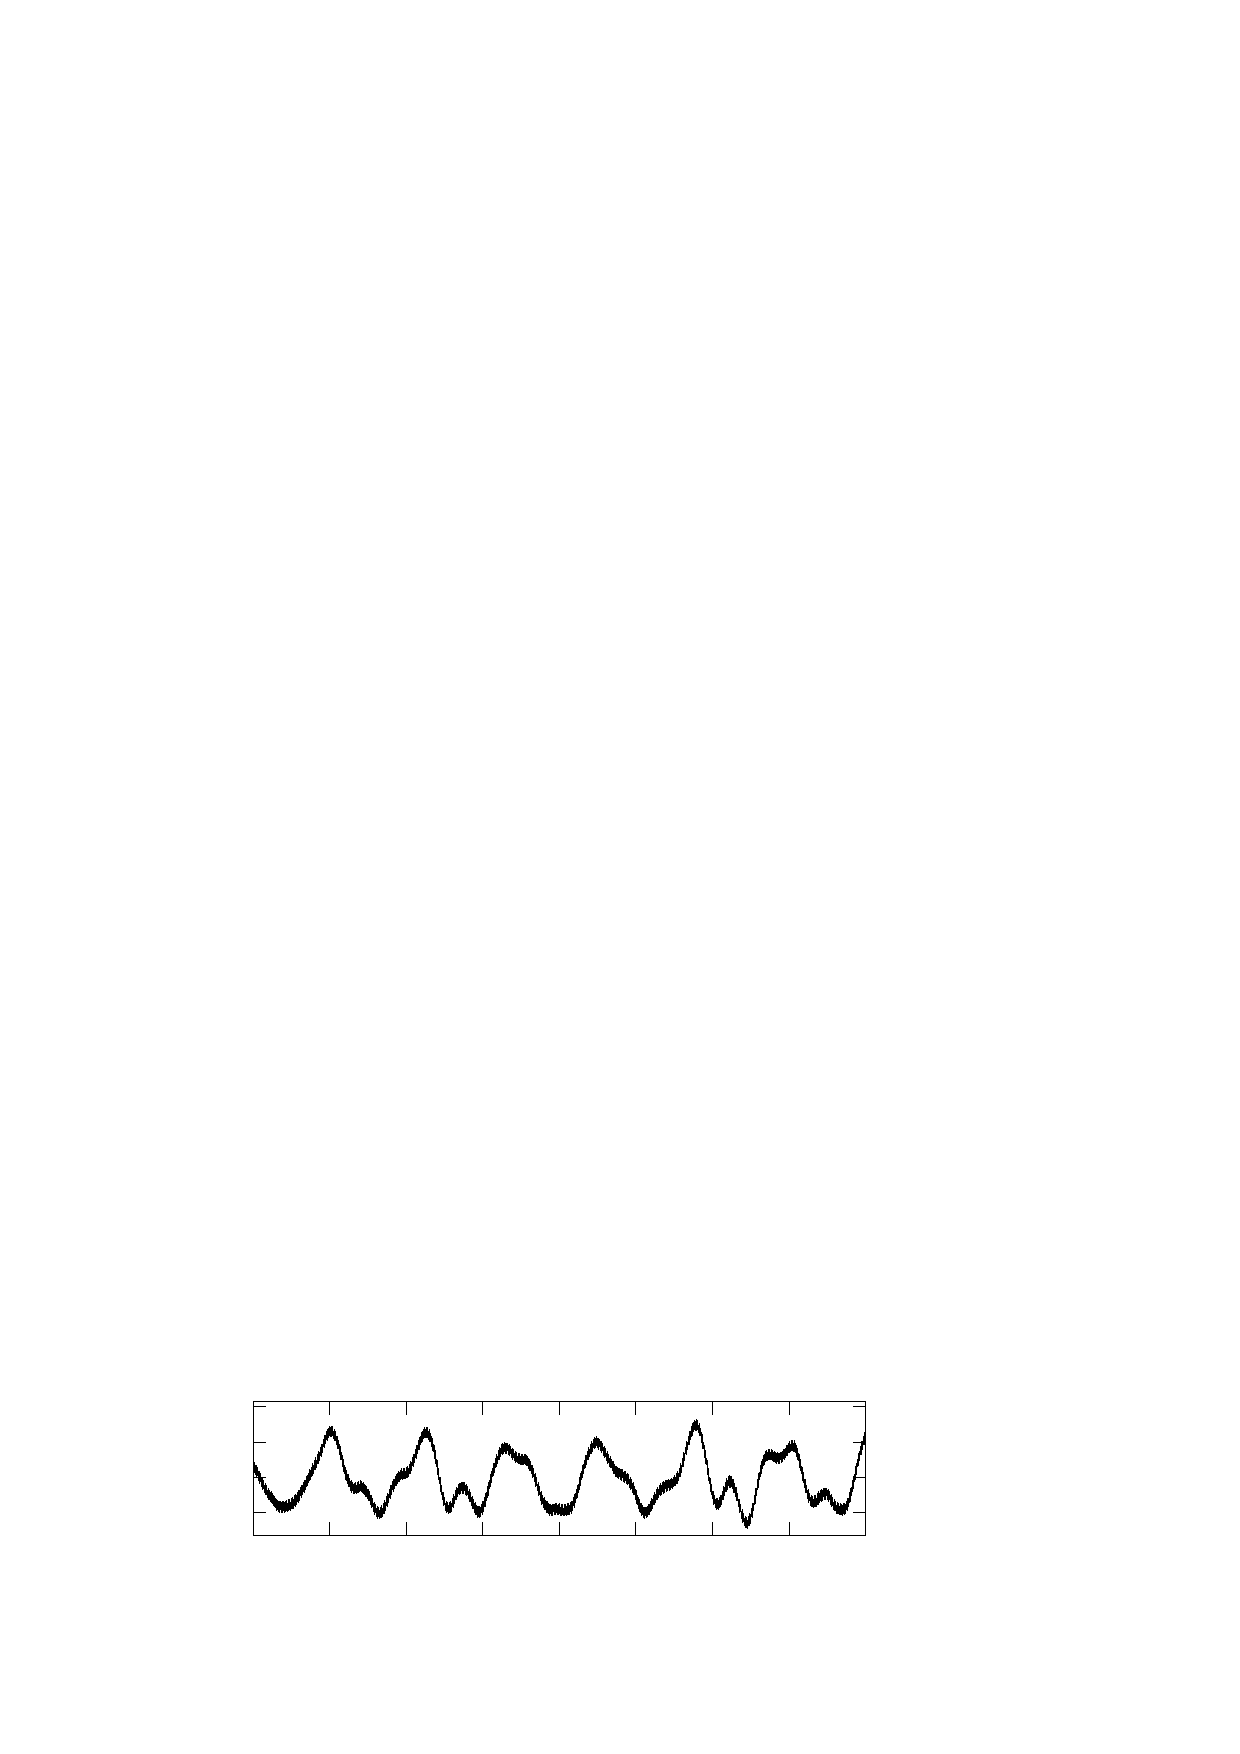
\includegraphics{rounded-rhop30-Fo5_631e-02}%
\end{picture}%
\begingroup
\setlength{\unitlength}{0.0200bp}%
\begin{picture}(18000,5400)(0,0)%
\put(2200,2193){\makebox(0,0)[r]{\strut{}1.40}}%
\put(2200,3040){\makebox(0,0)[r]{\strut{}1.50}}%
\put(2200,3887){\makebox(0,0)[r]{\strut{}1.60}}%
\put(2200,4734){\makebox(0,0)[r]{\strut{}1.70}}%
\put(2475,1100){\makebox(0,0){\strut{} 1600}}%
\put(4313,1100){\makebox(0,0){\strut{} 1650}}%
\put(6150,1100){\makebox(0,0){\strut{} 1700}}%
\put(7988,1100){\makebox(0,0){\strut{} 1750}}%
\put(9825,1100){\makebox(0,0){\strut{} 1800}}%
\put(11663,1100){\makebox(0,0){\strut{} 1850}}%
\put(13500,1100){\makebox(0,0){\strut{} 1900}}%
\put(15338,1100){\makebox(0,0){\strut{} 1950}}%
\put(17175,1100){\makebox(0,0){\strut{} 2000}}%
\put(550,3250){\rotatebox{90}{\makebox(0,0){\strut{}$y^\ast$}}}%
\put(9825,275){\makebox(0,0){\strut{}$t^\ast$}}%
\put(600,1000){\rotatebox{0}{\makebox(0,0){\strut{}(a)}}}%
\end{picture}%
\endgroup
\endinput

%GNUPLOT: LaTeX picture with Postscript
\begin{picture}(0,0)%
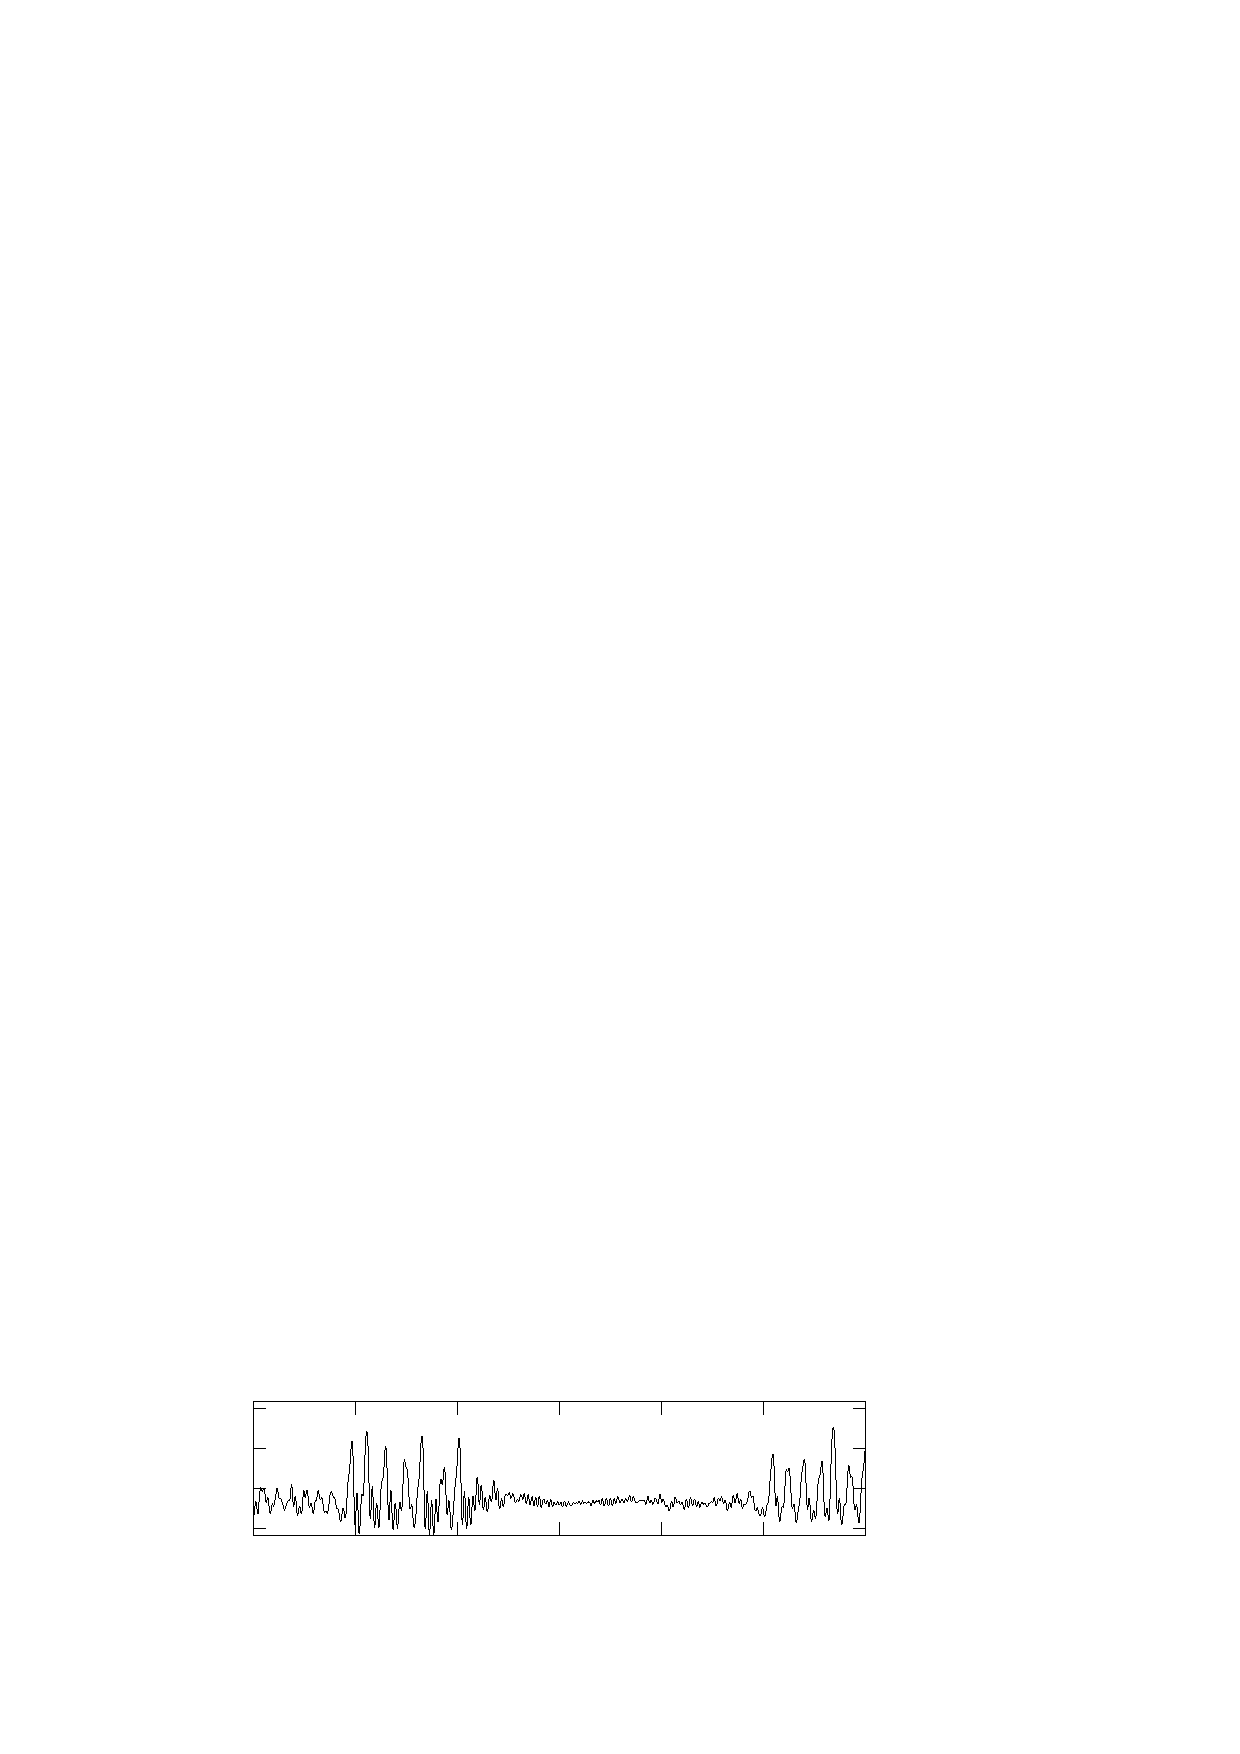
\includegraphics{rounded-rhop30-Fo8_072e-02}%
\end{picture}%
\begingroup
\setlength{\unitlength}{0.0200bp}%
\begin{picture}(18000,5400)(0,0)%
\put(2200,1805){\makebox(0,0)[r]{\strut{}1.20}}%
\put(2200,2765){\makebox(0,0)[r]{\strut{}1.60}}%
\put(2200,3725){\makebox(0,0)[r]{\strut{}2.00}}%
\put(2200,4685){\makebox(0,0)[r]{\strut{}2.40}}%
\put(2475,1100){\makebox(0,0){\strut{} 500}}%
\put(4925,1100){\makebox(0,0){\strut{} 1000}}%
\put(7375,1100){\makebox(0,0){\strut{} 1500}}%
\put(9825,1100){\makebox(0,0){\strut{} 2000}}%
\put(12275,1100){\makebox(0,0){\strut{} 2500}}%
\put(14725,1100){\makebox(0,0){\strut{} 3000}}%
\put(17175,1100){\makebox(0,0){\strut{} 3500}}%
\put(550,3250){\rotatebox{90}{\makebox(0,0){\strut{}$y^\ast$}}}%
\put(9825,275){\makebox(0,0){\strut{}$t^\ast$}}%
\put(600,1000){\rotatebox{0}{\makebox(0,0){\strut{}(c)}}}%
\end{picture}%
\endgroup
\endinput

\caption{\label{fig:paths-rho-30-rounded}
Trayectoria vertical de la part'icula s'olida $\rho_p/\rho_f=50$ sobre el tiempo en la cavidad redondeada para
(a) $P_o^\ast = 6.0\times 10^{-4} $,
%(b) $P_o^\ast = 2.55\times 10^{-3}$,
(b) $P_o^\ast = 4.5\times 10^{-3}$
y
(c) $P_o^\ast = 6.45\times 10^{-3}$.
}
\end{figure}
%
\begin{figure}
%%GNUPLOT: LaTeX picture with Postscript
%\begin{picture}(0,0)%
%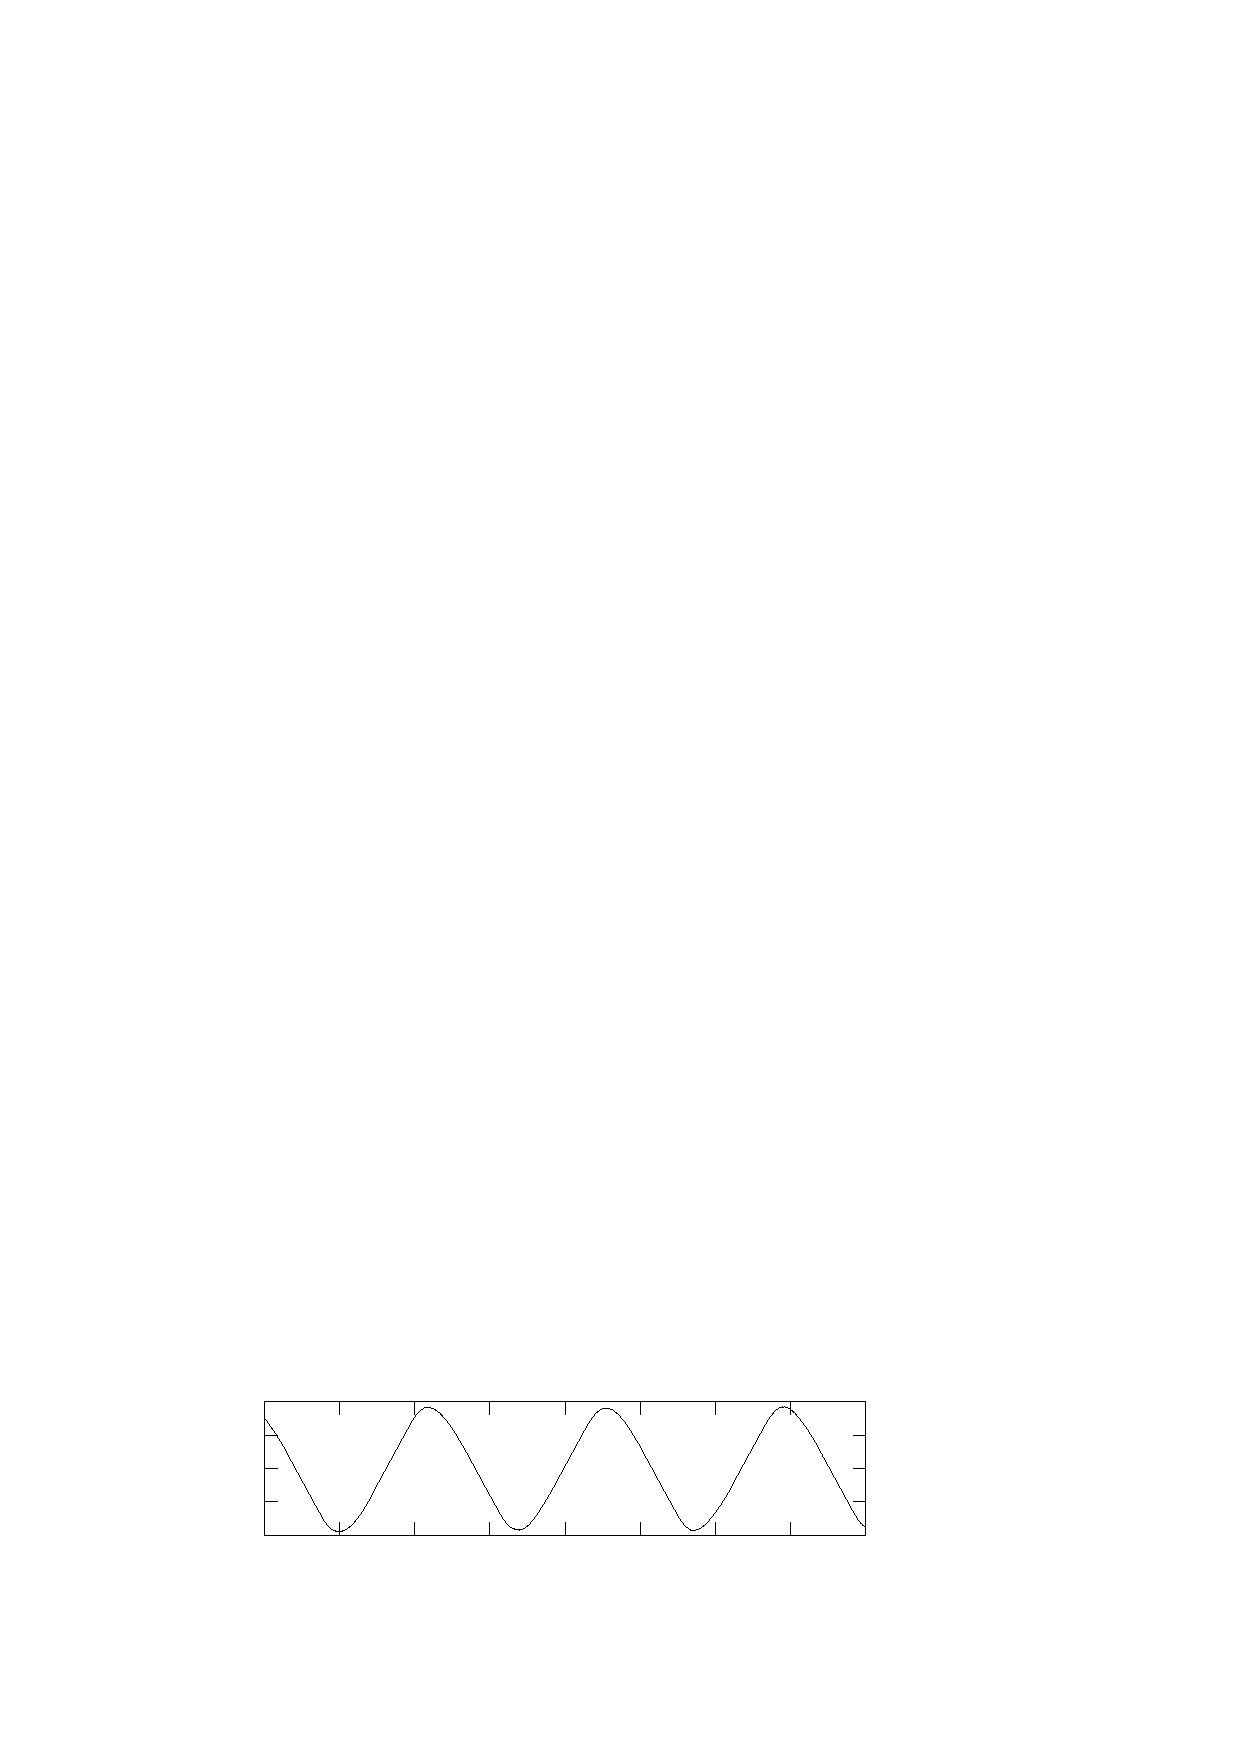
\includegraphics{rounded-rhop30-Fo5_631e-02-x}%
%\end{picture}%
%\begingroup
%\setlength{\unitlength}{0.0200bp}%
%\begin{picture}(18000,5400)(0,0)%
%\put(2475,1650){\makebox(0,0)[r]{\strut{}-1.60}}%
%\put(2475,2450){\makebox(0,0)[r]{\strut{}-0.80}}%
%\put(2475,3250){\makebox(0,0)[r]{\strut{}0.00}}%
%\put(2475,4050){\makebox(0,0)[r]{\strut{}0.80}}%
%\put(2475,4850){\makebox(0,0)[r]{\strut{}1.60}}%
%\put(2750,1100){\makebox(0,0){\strut{} 1600}}%
%\put(4553,1100){\makebox(0,0){\strut{} 1650}}%
%\put(6356,1100){\makebox(0,0){\strut{} 1700}}%
%\put(8159,1100){\makebox(0,0){\strut{} 1750}}%
%\put(9963,1100){\makebox(0,0){\strut{} 1800}}%
%\put(11766,1100){\makebox(0,0){\strut{} 1850}}%
%\put(13569,1100){\makebox(0,0){\strut{} 1900}}%
%\put(15372,1100){\makebox(0,0){\strut{} 1950}}%
%\put(17175,1100){\makebox(0,0){\strut{} 2000}}%
%\put(550,3250){\rotatebox{90}{\makebox(0,0){\strut{}$x^\ast$}}}%
%\put(9962,275){\makebox(0,0){\strut{}$t^\ast$}}%
%\put(600,1000){\rotatebox{0}{\makebox(0,0){\strut{}(b)}}}%
%\end{picture}%
%\endgroup
%\endinput

%GNUPLOT: LaTeX picture with Postscript
\begin{picture}(0,0)%
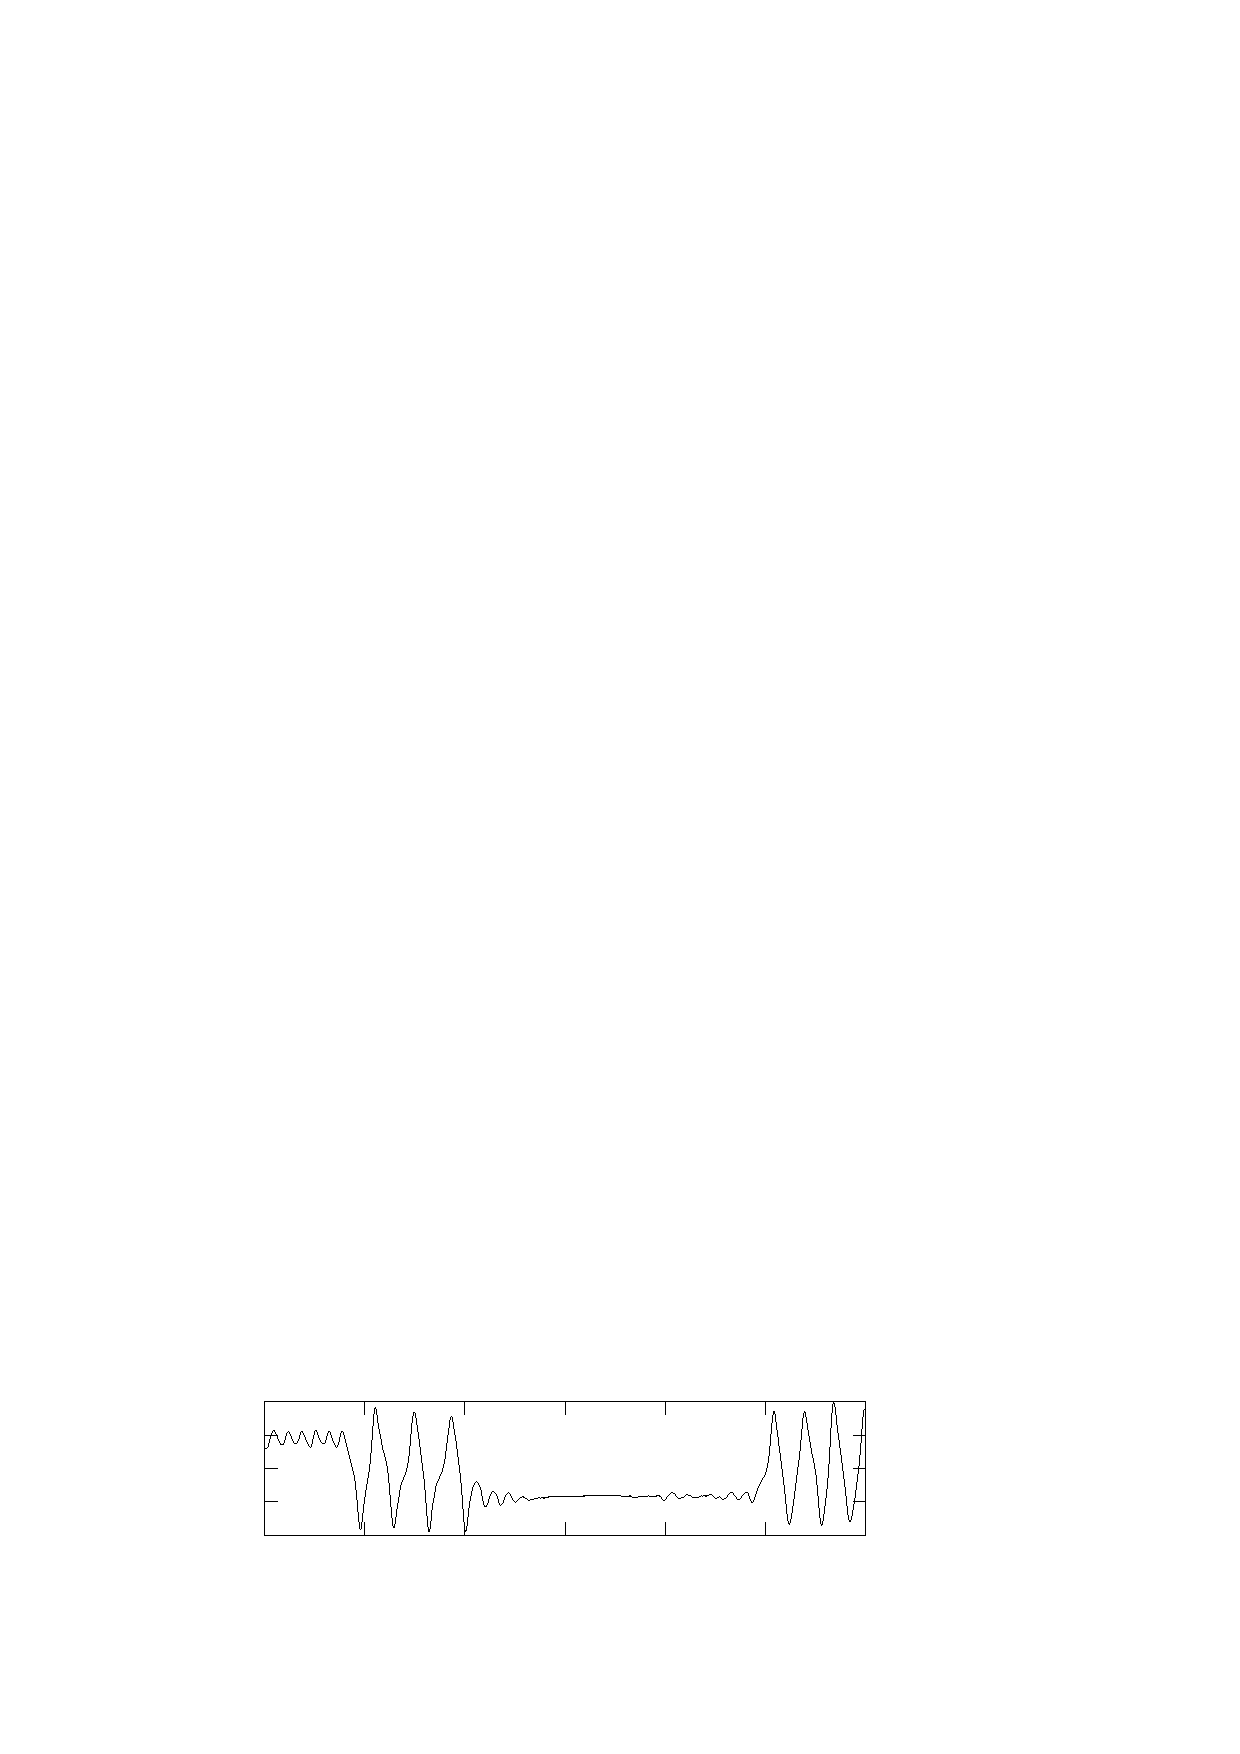
\includegraphics{rounded-rhop30-Fo8_072e-02-x}%
\end{picture}%
\begingroup
\setlength{\unitlength}{0.0200bp}%
\begin{picture}(18000,5400)(0,0)%
\put(2475,1650){\makebox(0,0)[r]{\strut{}-2.80}}%
\put(2475,2450){\makebox(0,0)[r]{\strut{}-1.40}}%
\put(2475,3250){\makebox(0,0)[r]{\strut{}0.00}}%
\put(2475,4050){\makebox(0,0)[r]{\strut{}1.40}}%
\put(2475,4850){\makebox(0,0)[r]{\strut{}2.80}}%
\put(3652,1100){\makebox(0,0){\strut{} 500}}%
\put(5905,1100){\makebox(0,0){\strut{} 1000}}%
\put(8159,1100){\makebox(0,0){\strut{} 1500}}%
\put(10413,1100){\makebox(0,0){\strut{} 2000}}%
\put(12667,1100){\makebox(0,0){\strut{} 2500}}%
\put(14921,1100){\makebox(0,0){\strut{} 3000}}%
\put(17175,1100){\makebox(0,0){\strut{} 3500}}%
\put(550,3250){\rotatebox{90}{\makebox(0,0){\strut{}$x^\ast$}}}%
\put(9962,275){\makebox(0,0){\strut{}$t^\ast$}}%
\put(600,1000){\rotatebox{0}{\makebox(0,0){\strut{}(d)}}}%
\end{picture}%
\endgroup
\endinput

\caption{\label{fig:paths-rho-30-rounded-x}
Trayectoria horizontal de la part'icula s'olida $\rho_p/\rho_f=50$ sobre el tiempo en la cavidad redondeada para
(a) $P_o^\ast = 4.5\times 10^{-3}$
y
(b) $P_o^\ast = 6.45\times 10^{-3}$. Las trayectorias corresponden a las mostradas en las 
figuras~\ref{fig:paths-rho-30-rounded} (b) y (c), respectivamente.
}
\end{figure}
\begin{figure}
%GNUPLOT: LaTeX picture with Postscript
\begin{picture}(0,0)%
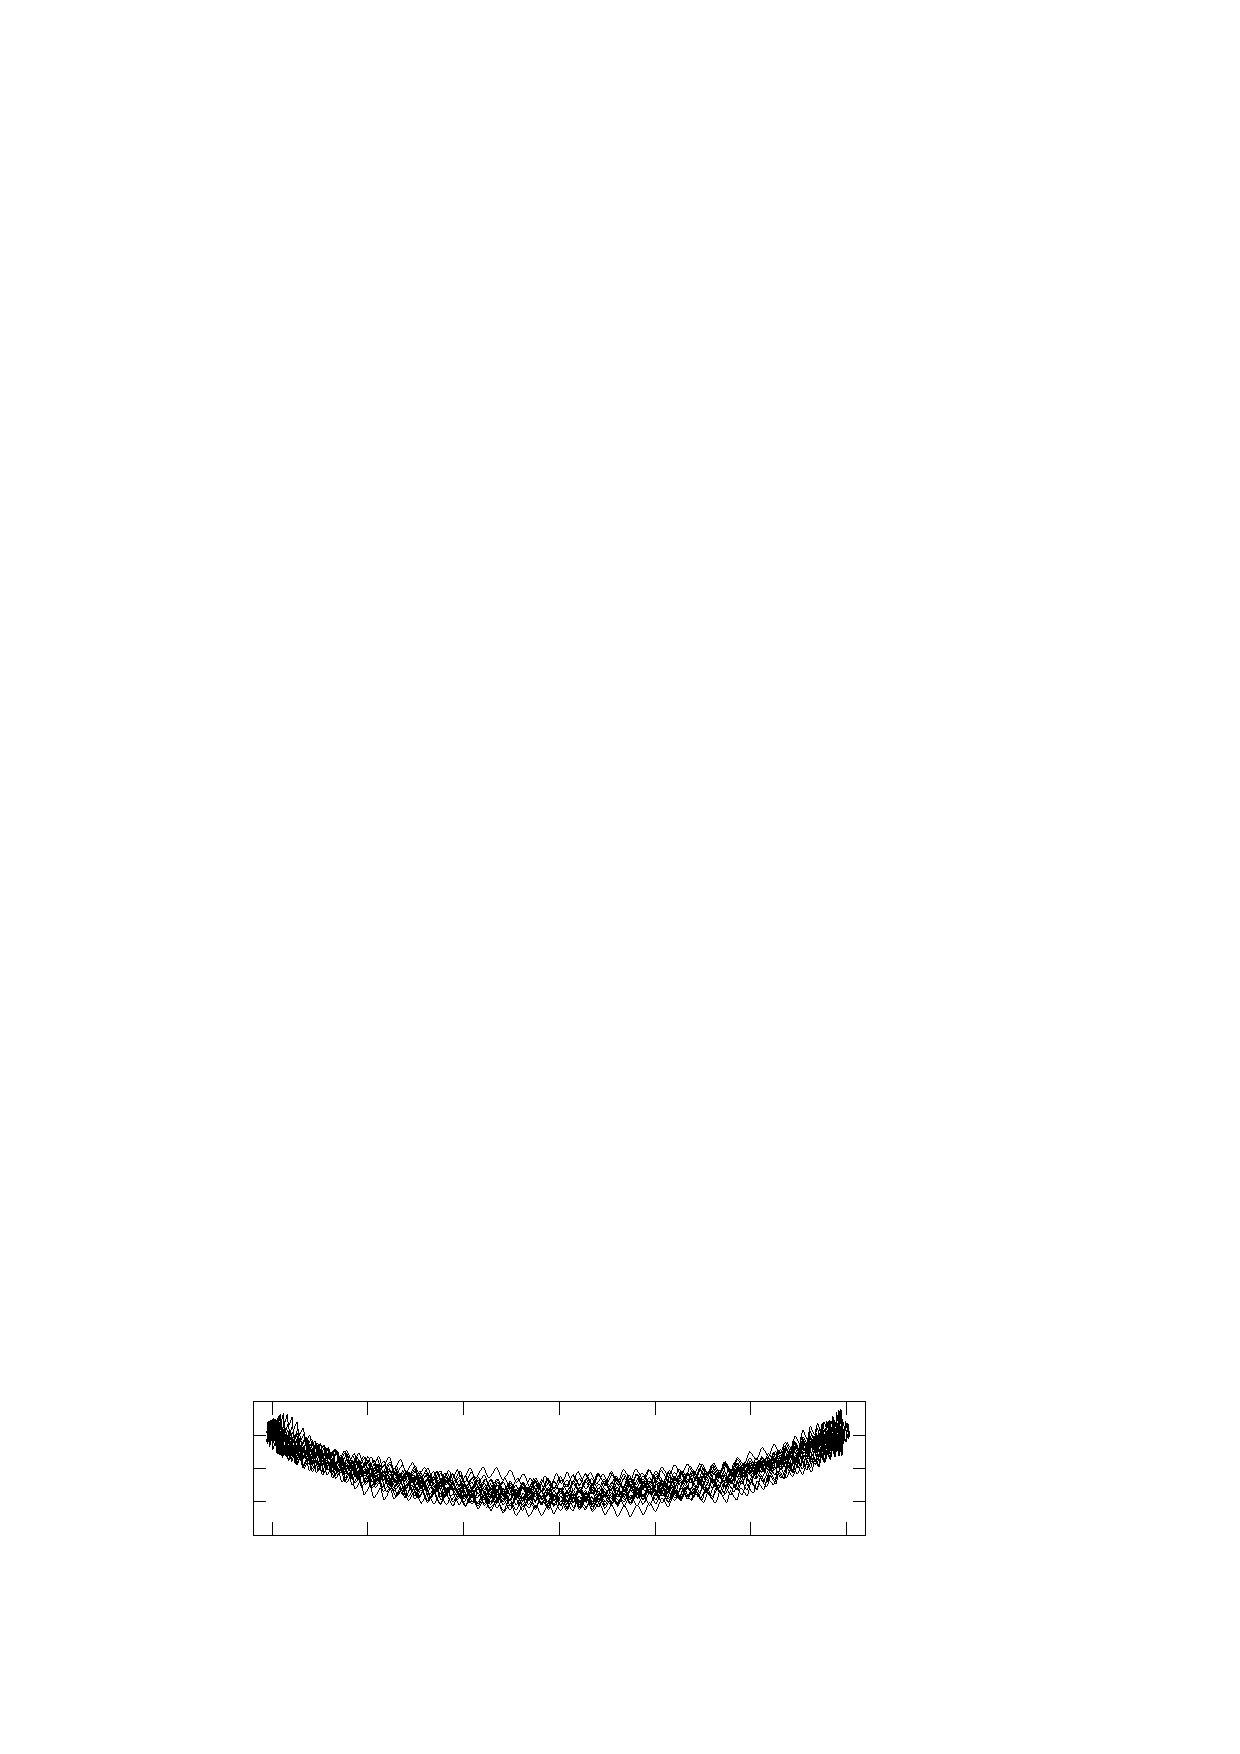
\includegraphics{eps/rounded-rhop30-Fo5_631e-02-x-y}%
\end{picture}%
\begingroup
\setlength{\unitlength}{0.0200bp}%
\begin{picture}(18000,5400)(0,0)%
\put(2200,1650){\makebox(0,0)[r]{\strut{}1.30}}%
\put(2200,2450){\makebox(0,0)[r]{\strut{}1.40}}%
\put(2200,3250){\makebox(0,0)[r]{\strut{}1.50}}%
\put(2200,4050){\makebox(0,0)[r]{\strut{}1.60}}%
\put(2200,4850){\makebox(0,0)[r]{\strut{}1.70}}%
\put(2934,1100){\makebox(0,0){\strut{}-1.5}}%
\put(5231,1100){\makebox(0,0){\strut{}-1}}%
\put(7528,1100){\makebox(0,0){\strut{}-0.5}}%
\put(9825,1100){\makebox(0,0){\strut{} 0}}%
\put(12122,1100){\makebox(0,0){\strut{} 0.5}}%
\put(14419,1100){\makebox(0,0){\strut{} 1}}%
\put(16716,1100){\makebox(0,0){\strut{} 1.5}}%
\put(550,3250){\rotatebox{90}{\makebox(0,0){\strut{}$y^\ast$}}}%
\put(9825,275){\makebox(0,0){\strut{}$x^\ast$}}%
\put(600,1000){\rotatebox{0}{\makebox(0,0){\strut{}(a)}}}%
\end{picture}%
\endgroup
\endinput

%%GNUPLOT: LaTeX picture with Postscript
%\begin{picture}(0,0)%
%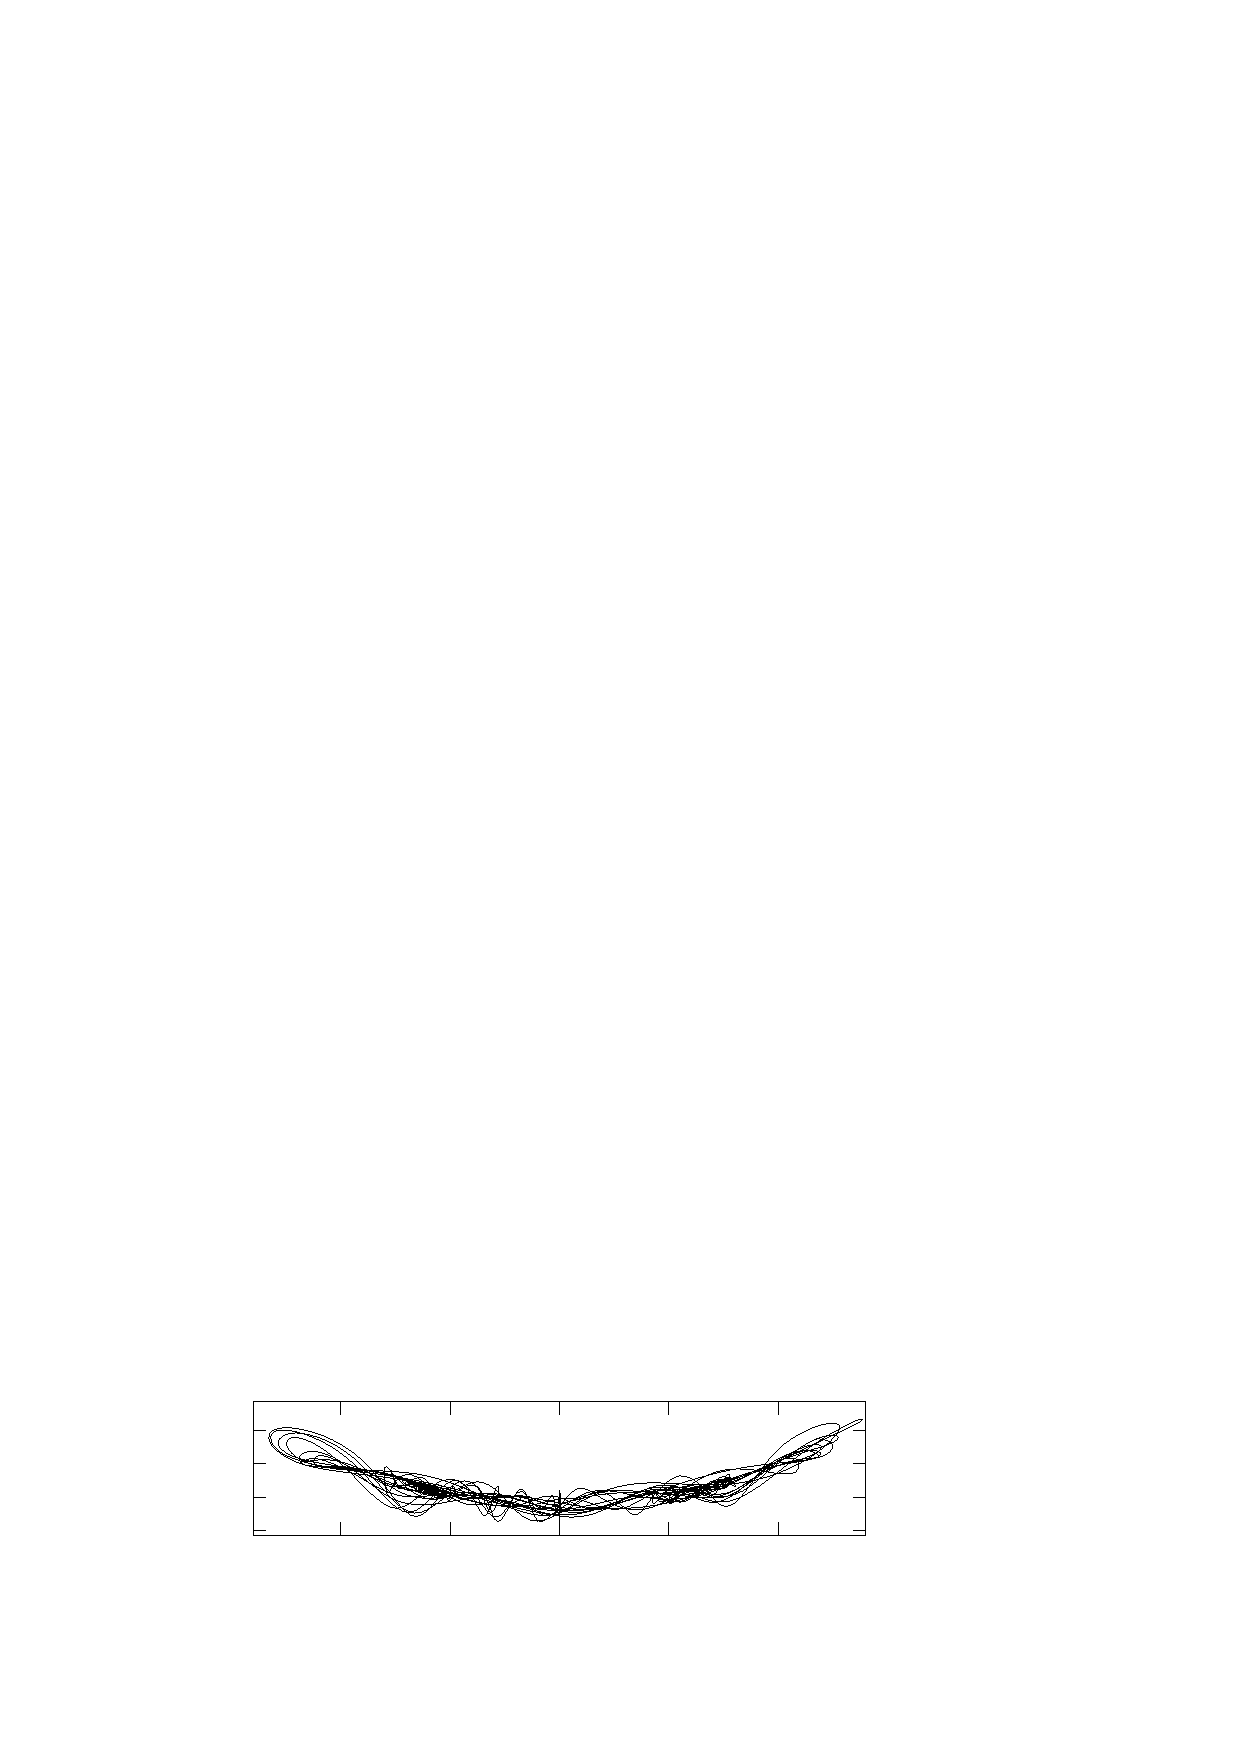
\includegraphics{rounded-rhop30-Fo8_072e-02-x-y}%
%\end{picture}%
%\begingroup
%\setlength{\unitlength}{0.0200bp}%
%\begin{picture}(18000,5400)(0,0)%
%\put(2200,1764){\makebox(0,0)[r]{\strut{}1.05}}%
%\put(2200,2564){\makebox(0,0)[r]{\strut{}1.40}}%
%\put(2200,3364){\makebox(0,0)[r]{\strut{}1.75}}%
%\put(2200,4164){\makebox(0,0)[r]{\strut{}2.10}}%
%\put(4575,1100){\makebox(0,0){\strut{}-2}}%
%\put(7200,1100){\makebox(0,0){\strut{}-1}}%
%\put(9825,1100){\makebox(0,0){\strut{} 0}}%
%\put(12450,1100){\makebox(0,0){\strut{} 1}}%
%\put(15075,1100){\makebox(0,0){\strut{} 2}}%
%\put(550,3250){\rotatebox{90}{\makebox(0,0){\strut{}$y^\ast$}}}%
%\put(9825,275){\makebox(0,0){\strut{}$x^\ast$}}%
%\put(600,1000){\rotatebox{0}{\makebox(0,0){\strut{}(b)}}}%
%\end{picture}%
%\endgroup
%\endinput

\caption{\label{fig:paths-rho-30-rounded-x-y} 
Trayectoria en el plano $x--y$ de la part'icula s'olida en la cavidad redondeada  para
(a) $P_o^\ast = 4.5\times 10^{-3}$
y
(b) $P_o^\ast = 6.45\times 10^{-3}$. Las trayectorias corresponden a las mostradas en las 
figuras~\ref{fig:paths-rho-30-rounded} (b) y (c), respectivamente.
}
\end{figure}
\begin{figure}
%\put(15400,4350){\makebox(0,0)[r]{\strut{}(b)}}%
%estan ~gbv/doctorado/levitation/particle/flat-cavity/spectrum/barrido-rho
%%GNUPLOT: LaTeX picture with Postscript
%\begin{picture}(0,0)%
%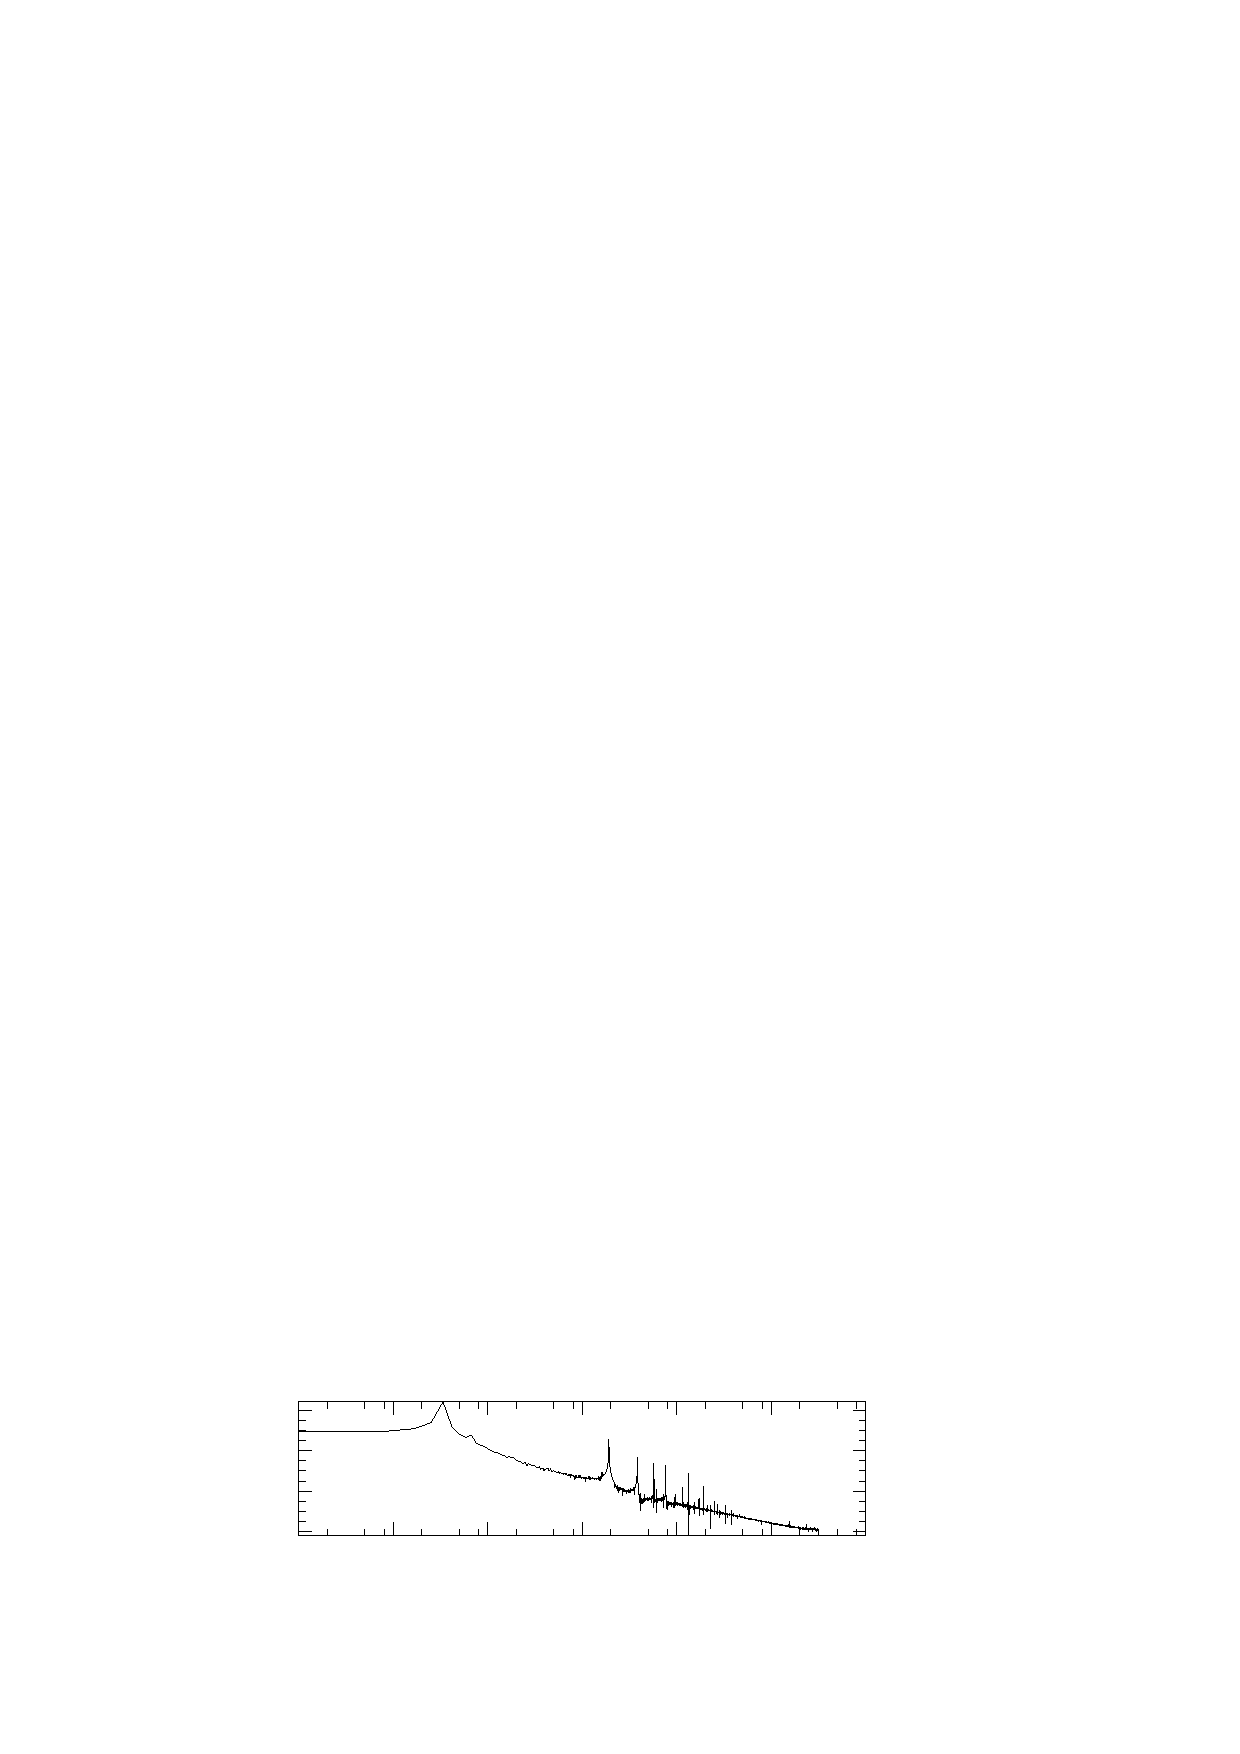
\includegraphics{rounded-rhop30-Fo7_508e-03-spectrum}%
%\end{picture}%
%\begingroup
%\setlength{\unitlength}{0.0200bp}%
%\begin{picture}(18000,5400)(0,0)%
%\put(3300,1750){\makebox(0,0)[r]{\strut{}1.00e-16}}%
%\put(3300,2712){\makebox(0,0)[r]{\strut{}1.00e-12}}%
%\put(3300,3674){\makebox(0,0)[r]{\strut{}1.00e-08}}%
%\put(3300,4636){\makebox(0,0)[r]{\strut{}1.00e-04}}%
%\put(3575,1100){\makebox(0,0){\strut{} 1e-05}}%
%\put(5842,1100){\makebox(0,0){\strut{} 1e-04}}%
%\put(8108,1100){\makebox(0,0){\strut{} 0.001}}%
%\put(10375,1100){\makebox(0,0){\strut{} 0.01}}%
%\put(12642,1100){\makebox(0,0){\strut{} 0.1}}%
%\put(14908,1100){\makebox(0,0){\strut{} 1}}%
%\put(17175,1100){\makebox(0,0){\strut{} 10}}%
%\put(550,3250){\rotatebox{90}{\makebox(0,0){\strut{}$PSD$}}}%
%\put(10375,275){\makebox(0,0){\strut{}$\omega$}}%
%\put(600,1000){\makebox(0,0){\strut{}(a)}}%
%\end{picture}%
%\endgroup
%\endinput

%%GNUPLOT: LaTeX picture with Postscript
\begin{picture}(0,0)%
\includegraphics{rounded-rhop30-Fo3_191e-02-spectrum}%
\end{picture}%
\begingroup
\setlength{\unitlength}{0.0200bp}%
\begin{picture}(18000,5400)(0,0)%
\put(3300,2123){\makebox(0,0)[r]{\strut{}3.20e-14}}%
\put(3300,2997){\makebox(0,0)[r]{\strut{}1.60e-11}}%
\put(3300,3871){\makebox(0,0)[r]{\strut{}8.00e-09}}%
\put(3300,4745){\makebox(0,0)[r]{\strut{}4.00e-06}}%
\put(3575,1100){\makebox(0,0){\strut{} 1e-05}}%
\put(5842,1100){\makebox(0,0){\strut{} 1e-04}}%
\put(8108,1100){\makebox(0,0){\strut{} 0.001}}%
\put(10375,1100){\makebox(0,0){\strut{} 0.01}}%
\put(12642,1100){\makebox(0,0){\strut{} 0.1}}%
\put(14908,1100){\makebox(0,0){\strut{} 1}}%
\put(17175,1100){\makebox(0,0){\strut{} 10}}%
\put(550,3250){\rotatebox{90}{\makebox(0,0){\strut{}$PSD$}}}%
\put(10375,275){\makebox(0,0){\strut{}$\omega$}}%
\end{picture}%
\endgroup
\endinput

%%GNUPLOT: LaTeX picture with Postscript
%\begin{picture}(0,0)%
%\includegraphics{rounded-rhop30-Fo5_631e-02-spectrum}%
%\end{picture}%
%\begingroup
%\setlength{\unitlength}{0.0200bp}%
%\begin{picture}(18000,5400)(0,0)%
%\put(3300,1850){\makebox(0,0)[r]{\strut{}3.20e-14}}%
%\put(3300,2601){\makebox(0,0)[r]{\strut{}1.60e-11}}%
%\put(3300,3352){\makebox(0,0)[r]{\strut{}8.00e-09}}%
%\put(3300,4103){\makebox(0,0)[r]{\strut{}4.00e-06}}%
%\put(3575,1100){\makebox(0,0){\strut{} 1e-05}}%
%\put(5842,1100){\makebox(0,0){\strut{} 1e-04}}%
%\put(8108,1100){\makebox(0,0){\strut{} 0.001}}%
%\put(10375,1100){\makebox(0,0){\strut{} 0.01}}%
%\put(12642,1100){\makebox(0,0){\strut{} 0.1}}%
%\put(14908,1100){\makebox(0,0){\strut{} 1}}%
%\put(17175,1100){\makebox(0,0){\strut{} 10}}%
%\put(550,3250){\rotatebox{90}{\makebox(0,0){\strut{}$PSD$}}}%
%\put(10375,275){\makebox(0,0){\strut{}$\omega$}}%
%\put(600,1000){\makebox(0,0){\strut{}(b)}}%
%\end{picture}%
%\endgroup
%\endinput

%%GNUPLOT: LaTeX picture with Postscript
%\begin{picture}(0,0)%
%\includegraphics{rounded-rhop30-Fo8_072e-02-spectrum}%
%\end{picture}%
%\begingroup
%\setlength{\unitlength}{0.0200bp}%
%\begin{picture}(18000,5400)(0,0)%
%\put(3300,1692){\makebox(0,0)[r]{\strut{}3.20e-14}}%
%\put(3300,2476){\makebox(0,0)[r]{\strut{}1.60e-11}}%
%\put(3300,3260){\makebox(0,0)[r]{\strut{}8.00e-09}}%
%\put(3300,4044){\makebox(0,0)[r]{\strut{}4.00e-06}}%
%\put(3300,4829){\makebox(0,0)[r]{\strut{}2.00e-03}}%
%\put(3575,1100){\makebox(0,0){\strut{} 1e-05}}%
%\put(5842,1100){\makebox(0,0){\strut{} 1e-04}}%
%\put(8108,1100){\makebox(0,0){\strut{} 0.001}}%
%\put(10375,1100){\makebox(0,0){\strut{} 0.01}}%
%\put(12642,1100){\makebox(0,0){\strut{} 0.1}}%
%\put(14908,1100){\makebox(0,0){\strut{} 1}}%
%\put(17175,1100){\makebox(0,0){\strut{} 10}}%
%\put(550,3250){\rotatebox{90}{\makebox(0,0){\strut{}$PSD$}}}%
%\put(10375,275){\makebox(0,0){\strut{}$\omega$}}%
%\put(600,1000){\rotatebox{0}{\makebox(0,0){\strut{}(c)}}}%
%\end{picture}%
%\endgroup
%\endinput

\caption{\label{fig:paths-rho-30-rounded-spectrum}
Espectro de potencia del movimiento vertical de la part'icula s'olida $\rho_p/\rho_f=50$ sobre el tiempo en la cavidad redondeada para
(a) $P_o^\ast = 6.0\times 10^{-4} $,
%(b) $P_o^\ast = 2.55\times 10^{-3}$,
(b) $P_o^\ast = 4.5\times 10^{-3}$
y
(c) $P_o^\ast = 6.45\times 10^{-3}$. Los espectros corresponden a las trayectorias mostradas en las 
figuras~\ref{fig:paths-rho-30-rounded} (a), (b) y (c).
}
\end{figure}
En las figuras~\ref{fig:paths-rho-30-rounded} (a), (b) y (c)  se muestra la posici'on vertical de la part'icula dentro de la
cavidad redondeada para $\rho_p/\rho_f = 50$ y (a) $P_o^\ast = 6.0\times 10^{-4} $, %(b) $P_o^\ast = 2.55\times 10^{-3}$,
(b) $P_o^\ast = 4.5\times 10^{-3}$ y (c) $P_o^\ast = 6.45\times 10^{-3}$. Todas las trayectorias de este conjunto de
simulaciones num'ericas tienen dos frecuencias en su movimiento. Una de ellas es la frecuencia de oscilaci'on
de la fuente ac'ustica y la segunda es una frecuencia m'as baja y con una amplitud m'as grande. Las 
figuras~\ref{fig:paths-rho-30-rounded} (b) y (c) corresponden a las simulaciones donde la amplitud de oscilaci'on
de la part'icula $\sigma_y$ crecen. Estas dos trayectorias  presentan un movimiento irregular, como se 
puede observar. Analizando el movimiento horizontal de la part'icula, mostrado en las figuras~\ref{fig:paths-rho-30-rounded-x} (a) y (b),
vemos que la part'icula comienza a oscilar tambi'en en el eje horizontal. Para la
trayectoria correspondiente a la figura~\ref{fig:paths-rho-30-rounded-x} (a), se observa un movimiento sinusoidal parala posici'on
horizontal de la part'icula. Para $P_o^\ast = 6.4\times 10^{-3}$ el movimiento horizontal de la part'icula,
mostrado en la figura~\ref{fig:paths-rho-30-rounded-x} (b), es muy irregular, la part'icula parece estacionarse en 
$x^\ast = 1.4$ para despu'es moverse hacia $x^\ast = -1.4$ y as'i sucesivamente. En las figuras~\ref{fig:paths-rho-30-rounded-x-y}
(a) y (b) se grafica la trayectoria de la part'icula en el plano $x-y$. Para $P^\ast_o = 4.5 \times 10^{-3}$ se aprecia un 
movimiento uniforme en forma de U dentro de la cavidad redondeada, figura~\ref{fig:paths-rho-30-rounded-x-y} (a). 
Para  $P^\ast_o = 6.45 \times 10^{-3}$, figura~\ref{fig:paths-rho-30-rounded-x-y} (b), la trayectoria presenta la misma
forma pero se ve m'as desordenada y se ven dos zonas por donde la part'icula pasa m'as veces ubicadas en
$(-1.4,1.5)$ y  $(1.4,1.5)$, donde la densidad de puntos indica que la part'icula pas'o por ah'i m'as veces. 
En las figuras~\ref{fig:paths-rho-30-rounded-spectrum} (a), (b) y (c) se muestran los espectros de potencia para 
las trayectorias mostradas en la figura~\ref{fig:paths-rho-30-rounded} (a), (b) y (c), respectivamente. 
En la figura~\ref{fig:paths-rho-30-rounded-spectrum} (a) se ve que el movimiento de la part'icula tiene dos frecuencias, la
correspondiente a la fuente ac'ustica con sus arm'onicos y la frecuencia m'as lenta que ha estado apareciendo. 
De la figura~\ref{fig:paths-rho-30-rounded-spectrum} (b) es dificil distinguir la segunda frecuencia para el movimiento
vertical de la part'icula, este espectro de potencia corresponde a la trayectoria donde la part'icula comienza a oscilar
de manera regular en el eje horizontal. La figura~\ref{fig:paths-rho-30-rounded-spectrum} (c) corresponde a la trayectoria
irregular en el eje horizontal y se aprecia la frecuencia de la fuente ac'ustica pero no hay otros 
picos bien definidos en el espectro de potencia. 
\begin{figure}
%\put(7200,1206){\makebox(0,0){\strut{} $x^\ast$}}%
%\put(4087,4289){\makebox(0,0)[r]{\strut{} $y^\ast$}}%
%\put(7200,1206){\makebox(0,0){\strut{} (a)}}%
\hskip -3.cm
%%GNUPLOT: LaTeX picture with Postscript
%\begin{picture}(0,0)%
%\includegraphics{variaciones-P-rho-30-Fo7_5e-03}%
%\end{picture}%
%\begingroup
%\setlength{\unitlength}{0.0200bp}%
%\begin{picture}(14400,8640)(0,0)%
%\put(10336,4426){\makebox(0,0)[l]{\strut{}1.000}}%
%\put(10336,5092){\makebox(0,0)[l]{\strut{}1.003}}%
%\put(10336,5757){\makebox(0,0)[l]{\strut{}1.005}}%
%\put(10336,6423){\makebox(0,0)[l]{\strut{}1.008}}%
%\put(9038,2206){\makebox(0,0){\strut{}-6}}%
%\put(8426,2206){\makebox(0,0){\strut{}-4}}%
%\put(7812,2206){\makebox(0,0){\strut{}-2}}%
%\put(7200,2206){\makebox(0,0){\strut{} 0}}%
%\put(6587,2206){\makebox(0,0){\strut{} 2}}%
%\put(5974,2206){\makebox(0,0){\strut{} 4}}%
%\put(5361,2206){\makebox(0,0){\strut{} 6}}%
%\put(5086,3063){\makebox(0,0)[r]{\strut{} 0}}%
%\put(5086,3676){\makebox(0,0)[r]{\strut{} 2}}%
%\put(5087,4289){\makebox(0,0)[r]{\strut{} 4}}%
%\put(5087,4901){\makebox(0,0)[r]{\strut{} 6}}%
%\put(5087,5514){\makebox(0,0)[r]{\strut{} 8}}%
%\put(5087,6127){\makebox(0,0)[r]{\strut{} 10}}%
%\put(7200,1206){\makebox(0,0){\strut{} $x^\ast$}}%
%\put(4087,4289){\makebox(0,0)[r]{\strut{} $y^\ast$}}%
%\put(12000,206){\makebox(0,0){\strut{} (a)}}%
%\end{picture}%
%\endgroup
%\endinput
 
\hskip -3.1cm
%%GNUPLOT: LaTeX picture with Postscript
%\begin{picture}(0,0)%
%\includegraphics{variaciones-U-rho-30-Fo7_5e-03}%
%\end{picture}%
%\begingroup
%\setlength{\unitlength}{0.0200bp}%
%\begin{picture}(14400,8640)(0,0)%
%\put(10336,4054){\makebox(0,0)[l]{\strut{}0.00}}%
%\put(10336,4646){\makebox(0,0)[l]{\strut{}0.25}}%
%\put(10336,5238){\makebox(0,0)[l]{\strut{}0.50}}%
%\put(10336,5830){\makebox(0,0)[l]{\strut{}0.75}}%
%\put(10336,6422){\makebox(0,0)[l]{\strut{}1.00}}%
%\put(9038,2206){\makebox(0,0){\strut{}-6}}%
%\put(8426,2206){\makebox(0,0){\strut{}-4}}%
%\put(7812,2206){\makebox(0,0){\strut{}-2}}%
%\put(7200,2206){\makebox(0,0){\strut{} 0}}%
%\put(6587,2206){\makebox(0,0){\strut{} 2}}%
%\put(5974,2206){\makebox(0,0){\strut{} 4}}%
%\put(5361,2206){\makebox(0,0){\strut{} 6}}%
%\put(5086,3063){\makebox(0,0)[r]{\strut{} 0}}%
%\put(5086,3676){\makebox(0,0)[r]{\strut{} 2}}%
%\put(5087,4289){\makebox(0,0)[r]{\strut{} 4}}%
%\put(5087,4901){\makebox(0,0)[r]{\strut{} 6}}%
%\put(5087,5514){\makebox(0,0)[r]{\strut{} 8}}%
%\put(5087,6127){\makebox(0,0)[r]{\strut{} 10}}%
%
%\put(7200,1206){\makebox(0,0){\strut{} $x^\ast$}}%
%\put(4087,4289){\makebox(0,0)[r]{\strut{} $y^\ast$}}%
%\end{picture}
%\endgroup
%\endinput
 

%\hskip -3.cm
%%GNUPLOT: LaTeX picture with Postscript
\begin{picture}(0,0)%
\includegraphics{variaciones-P-rho-30-Fo3_2e-02}%
\end{picture}%
\begingroup
\setlength{\unitlength}{0.0200bp}%
\begin{picture}(14400,8640)(0,0)%
\put(10336,4610){\makebox(0,0)[l]{\strut{}1.007}}%
\put(10336,5183){\makebox(0,0)[l]{\strut{}1.019}}%
\put(10336,5755){\makebox(0,0)[l]{\strut{}1.031}}%
\put(10336,6328){\makebox(0,0)[l]{\strut{}1.043}}%
\put(9038,2206){\makebox(0,0){\strut{}-6}}%
\put(8425,2206){\makebox(0,0){\strut{}-4}}%
\put(7812,2206){\makebox(0,0){\strut{}-2}}%
\put(7200,2206){\makebox(0,0){\strut{} 0}}%
\put(6587,2207){\makebox(0,0){\strut{} 2}}%
\put(5974,2207){\makebox(0,0){\strut{} 4}}%
\put(5361,2207){\makebox(0,0){\strut{} 6}}%
\put(5086,3063){\makebox(0,0)[r]{\strut{} 0}}%
\put(5086,3676){\makebox(0,0)[r]{\strut{} 2}}%
\put(5087,4289){\makebox(0,0)[r]{\strut{} 4}}%
\put(5087,4901){\makebox(0,0)[r]{\strut{} 6}}%
\put(5087,5514){\makebox(0,0)[r]{\strut{} 8}}%
\put(5087,6127){\makebox(0,0)[r]{\strut{} 10}}%
\end{picture}%
\endgroup
\endinput
 
%\hskip -3.1cm
%%GNUPLOT: LaTeX picture with Postscript
\begin{picture}(0,0)%
\includegraphics{variaciones-U-rho-30-Fo3_2e-02}%
\end{picture}%
\begingroup
\setlength{\unitlength}{0.0200bp}%
\begin{picture}(14400,8640)(0,0)%
\put(10336,4054){\makebox(0,0)[l]{\strut{}0.00}}%
\put(10336,4646){\makebox(0,0)[l]{\strut{}0.25}}%
\put(10336,5238){\makebox(0,0)[l]{\strut{}0.50}}%
\put(10336,5830){\makebox(0,0)[l]{\strut{}0.75}}%
\put(10336,6422){\makebox(0,0)[l]{\strut{}1.00}}%
\put(9038,2206){\makebox(0,0){\strut{}-6}}%
\put(8425,2206){\makebox(0,0){\strut{}-4}}%
\put(7812,2206){\makebox(0,0){\strut{}-2}}%
\put(7200,2206){\makebox(0,0){\strut{} 0}}%
\put(6587,2207){\makebox(0,0){\strut{} 2}}%
\put(5974,2207){\makebox(0,0){\strut{} 4}}%
\put(5361,2207){\makebox(0,0){\strut{} 6}}%
\put(5086,3063){\makebox(0,0)[r]{\strut{} 0}}%
\put(5086,3676){\makebox(0,0)[r]{\strut{} 2}}%
\put(5087,4289){\makebox(0,0)[r]{\strut{} 4}}%
\put(5087,4901){\makebox(0,0)[r]{\strut{} 6}}%
\put(5087,5514){\makebox(0,0)[r]{\strut{} 8}}%
\put(5087,6127){\makebox(0,0)[r]{\strut{} 10}}%
\end{picture}%
\endgroup
\endinput
 

\hskip -3.cm
%%GNUPLOT: LaTeX picture with Postscript
%\begin{picture}(0,0)%
%\includegraphics{variaciones-P-rho-30-Fo5_6e-02}%
%\end{picture}%
%\begingroup
%\setlength{\unitlength}{0.0200bp}%
%\begin{picture}(14400,8640)(0,0)%
%\put(10336,4623){\makebox(0,0)[l]{\strut{}1.016}}%
%\put(10336,5219){\makebox(0,0)[l]{\strut{}1.039}}%
%\put(10336,5815){\makebox(0,0)[l]{\strut{}1.061}}%
%\put(10336,6410){\makebox(0,0)[l]{\strut{}1.084}}%
%\put(9038,2206){\makebox(0,0){\strut{}-6}}%
%\put(8426,2206){\makebox(0,0){\strut{}-4}}%
%\put(7812,2206){\makebox(0,0){\strut{}-2}}%
%\put(7200,2206){\makebox(0,0){\strut{} 0}}%
%\put(6587,2206){\makebox(0,0){\strut{} 2}}%
%\put(5974,2206){\makebox(0,0){\strut{} 4}}%
%\put(5361,2206){\makebox(0,0){\strut{} 6}}%
%\put(5086,3063){\makebox(0,0)[r]{\strut{} 0}}%
%\put(5086,3676){\makebox(0,0)[r]{\strut{} 2}}%
%\put(5087,4289){\makebox(0,0)[r]{\strut{} 4}}%
%\put(5087,4901){\makebox(0,0)[r]{\strut{} 6}}%
%\put(5087,5514){\makebox(0,0)[r]{\strut{} 8}}%
%\put(5087,6127){\makebox(0,0)[r]{\strut{} 10}}%
%
%\put(7200,1206){\makebox(0,0){\strut{} $x^\ast$}}%
%\put(4087,4289){\makebox(0,0)[r]{\strut{} $y^\ast$}}%
%\put(12000,206){\makebox(0,0){\strut{} (b)}}%
%\end{picture}%
%\endgroup
%\endinput
 
\hskip -3.1cm
%%GNUPLOT: LaTeX picture with Postscript
%\begin{picture}(0,0)%
%\includegraphics{variaciones-U-rho-30-Fo5_6e-02}%
%\end{picture}%
%\begingroup
%\setlength{\unitlength}{0.0200bp}%
%\begin{picture}(14400,8640)(0,0)%
%\put(10336,4054){\makebox(0,0)[l]{\strut{}0.00}}%
%\put(10336,4646){\makebox(0,0)[l]{\strut{}0.25}}%
%\put(10336,5238){\makebox(0,0)[l]{\strut{}0.50}}%
%\put(10336,5830){\makebox(0,0)[l]{\strut{}0.75}}%
%\put(10336,6422){\makebox(0,0)[l]{\strut{}1.00}}%
%\put(9038,2206){\makebox(0,0){\strut{}-6}}%
%\put(8426,2206){\makebox(0,0){\strut{}-4}}%
%\put(7812,2206){\makebox(0,0){\strut{}-2}}%
%\put(7200,2206){\makebox(0,0){\strut{} 0}}%
%\put(6587,2206){\makebox(0,0){\strut{} 2}}%
%\put(5974,2206){\makebox(0,0){\strut{} 4}}%
%\put(5361,2206){\makebox(0,0){\strut{} 6}}%
%\put(5086,3063){\makebox(0,0)[r]{\strut{} 0}}%
%\put(5086,3676){\makebox(0,0)[r]{\strut{} 2}}%
%\put(5087,4289){\makebox(0,0)[r]{\strut{} 4}}%
%\put(5087,4901){\makebox(0,0)[r]{\strut{} 6}}%
%\put(5087,5514){\makebox(0,0)[r]{\strut{} 8}}%
%\put(5087,6127){\makebox(0,0)[r]{\strut{} 10}}%
%
%\put(7200,1206){\makebox(0,0){\strut{} $x^\ast$}}%
%\put(4087,4289){\makebox(0,0)[r]{\strut{} $y^\ast$}}%
%%\put(7200,1206){\makebox(0,0){\strut{} (a)}}%
%\end{picture}%
%\endgroup
%\endinput
 


\hskip -3.cm
%%GNUPLOT: LaTeX picture with Postscript
%\begin{picture}(0,0)%
%\includegraphics{variaciones-P-rho-30-Fo8_1e-02}%
%\end{picture}%
%\begingroup
%\setlength{\unitlength}{0.0200bp}%
%\begin{picture}(14400,8640)(0,0)%
%\put(10336,4530){\makebox(0,0)[l]{\strut{}1.012}}%
%\put(10336,5125){\makebox(0,0)[l]{\strut{}1.040}}%
%\put(10336,5719){\makebox(0,0)[l]{\strut{}1.068}}%
%\put(10336,6314){\makebox(0,0)[l]{\strut{}1.095}}%
%\put(9038,2206){\makebox(0,0){\strut{}-6}}%
%\put(8426,2206){\makebox(0,0){\strut{}-4}}%
%\put(7812,2206){\makebox(0,0){\strut{}-2}}%
%\put(7200,2206){\makebox(0,0){\strut{} 0}}%
%\put(6587,2206){\makebox(0,0){\strut{} 2}}%
%\put(5974,2206){\makebox(0,0){\strut{} 4}}%
%\put(5361,2206){\makebox(0,0){\strut{} 6}}%
%\put(5086,3063){\makebox(0,0)[r]{\strut{} 0}}%
%\put(5086,3676){\makebox(0,0)[r]{\strut{} 2}}%
%\put(5087,4289){\makebox(0,0)[r]{\strut{} 4}}%
%\put(5087,4901){\makebox(0,0)[r]{\strut{} 6}}%
%\put(5087,5514){\makebox(0,0)[r]{\strut{} 8}}%
%\put(5087,6127){\makebox(0,0)[r]{\strut{} 10}}%
%
%\put(7200,1206){\makebox(0,0){\strut{} $x^\ast$}}%
%\put(4087,4289){\makebox(0,0)[r]{\strut{} $y^\ast$}}%
%\put(12000,206){\makebox(0,0){\strut{} (c)}}%
%\end{picture}%
%\endgroup
%\endinput
 
\hskip -3.1cm
%%GNUPLOT: LaTeX picture with Postscript
%\begin{picture}(0,0)%
%\includegraphics{variaciones-U-rho-30-Fo8_1e-02}%
%\end{picture}%
%\begingroup
%\setlength{\unitlength}{0.0200bp}%
%\begin{picture}(14400,8640)(0,0)%
%\put(10336,4054){\makebox(0,0)[l]{\strut{}0.00}}%
%\put(10336,4646){\makebox(0,0)[l]{\strut{}0.25}}%
%\put(10336,5238){\makebox(0,0)[l]{\strut{}0.50}}%
%\put(10336,5830){\makebox(0,0)[l]{\strut{}0.75}}%
%\put(10336,6422){\makebox(0,0)[l]{\strut{}1.00}}%
%\put(9038,2206){\makebox(0,0){\strut{}-6}}%
%\put(8426,2206){\makebox(0,0){\strut{}-4}}%
%\put(7812,2206){\makebox(0,0){\strut{}-2}}%
%\put(7200,2206){\makebox(0,0){\strut{} 0}}%
%\put(6587,2206){\makebox(0,0){\strut{} 2}}%
%\put(5974,2206){\makebox(0,0){\strut{} 4}}%
%\put(5361,2206){\makebox(0,0){\strut{} 6}}%
%\put(5086,3063){\makebox(0,0)[r]{\strut{} 0}}%
%\put(5086,3676){\makebox(0,0)[r]{\strut{} 2}}%
%\put(5087,4289){\makebox(0,0)[r]{\strut{} 4}}%
%\put(5087,4901){\makebox(0,0)[r]{\strut{} 6}}%
%\put(5087,5514){\makebox(0,0)[r]{\strut{} 8}}%
%\put(5087,6127){\makebox(0,0)[r]{\strut{} 10}}%
%
%\put(7200,1206){\makebox(0,0){\strut{} $x^\ast$}}%
%\put(4087,4289){\makebox(0,0)[r]{\strut{} $y^\ast$}}%
%%\put(7200,1206){\makebox(0,0){\strut{} (a)}}%
%\end{picture}%
%\endgroup
%\endinput
 
%
%
%
\caption{\label{fig:potentials-rounded-rho-30}
Amplitud de las oscilaci'ones en la presi'on y la velocidad de izquierda a derecha para
(a) $P_o^\ast = 6.0\times 10^{-4} $,
%(b) $P_o^\ast = 2.55\times 10^{-3}$,
(b) $P_o^\ast = 4.5\times 10^{-3}$
y
(c) $P_o^\ast = 6.45\times 10^{-3}$.
}
\end{figure}
Finalmente, en las figuras~\ref{fig:potentials-rounded-rho-30} (a), (b) y (c) se muestran la amplitud de las oscilaciones  locales
de la presi'on y velocidad para $P_o^\ast = 6.0\times 10^{-4} $, $P_o^\ast = 4.5\times 10^{-3}$
y $P_o^\ast = 6.45\times 10^{-3}$, respectivamente. En la  figura~\ref{fig:potentials-rounded-rho-30} (a) 
se pueden apreciar los nodos de presi'on y los antinodos de velocidad. Estos nodos de presi'on se hacen
un poco m'as largos para  $P_o^\ast = 4.5\times 10^{-3}$, figura~\ref{fig:potentials-rounded-rho-30} (b), para
finalmente dividirse y formar dos nodos de presi'on a la misma altura, como se
puede observar en la  figura~\ref{fig:potentials-rounded-rho-30} (c) para  $P_o^\ast = 6.45\times 10^{-3}$. A pesar
de la formaci'on de dos nodos de presi'on, no ocurre lo mismo con el antinodo de velocidad, sin embargo, las zonas
donde se localizan los nuevos nodos de presi'on son zonas de alta velocidad, como se puede apreciar. La aparici'on de estos
dos nodos de presi'on explica el movimiento irregular de la part'icula para $P^\ast_o = 6.45 \times 10^{-3}$. La part'icula
fue liberada en $(0,1.2)$ dentro de la cavidad redondeada, y la part'icula se pasa de un nodo de presi'on a otro
sin estacionarse en cualquiera de los dos. En todos los experimentos anteriores, la part'icula se liber'o
en el centro de la cavidad a una altura  $y^\ast = 1.2$. Como se observa de la 
figura~\ref{fig:potentials-rounded-rho-30} (c), el nodo de presi'on ya no se encuentra en esa posici'on. Se realiz'o
una segunda simulaci'on num'erica con   $P_o^\ast = 6.45\times 10^{-3}$ y $\rho_p/\rho_f=50$ pero esta vez se 
coloc'o en uno de los nodos de presi'on $(-2,1.2)$ para ver si el movimiento de la part'icula en el eje horizontal
era funci'on de la posici'on inicial. En la figura~\ref{fig:paths-rho-30-rounded-x2} se muestra la trayectoria
de la part'icula en el eje horizontal cuando es liberada cerca del nodo de presi'on. De esta figura se observa que hay
oscilaciones grandes y que estas no dependen de la posici'on inicial. 
\begin{figure}
%GNUPLOT: LaTeX picture with Postscript
\begin{picture}(0,0)%
\includegraphics{rounded-rhop30-Fo8_072e-02-x2}%
\end{picture}%
\begingroup
\setlength{\unitlength}{0.0200bp}%
\begin{picture}(18000,5400)(0,0)%
\put(1650,1650){\makebox(0,0)[r]{\strut{}-4}}%
\put(1650,2450){\makebox(0,0)[r]{\strut{}-2}}%
\put(1650,3250){\makebox(0,0)[r]{\strut{} 0}}%
\put(1650,4050){\makebox(0,0)[r]{\strut{} 2}}%
\put(1650,4850){\makebox(0,0)[r]{\strut{} 4}}%
\put(1925,1100){\makebox(0,0){\strut{} 0}}%
\put(4975,1100){\makebox(0,0){\strut{} 4000}}%
\put(8025,1100){\makebox(0,0){\strut{} 8000}}%
\put(11075,1100){\makebox(0,0){\strut{} 12000}}%
\put(14125,1100){\makebox(0,0){\strut{} 16000}}%
\put(17175,1100){\makebox(0,0){\strut{} 20000}}%
\put(550,3250){\rotatebox{90}{\makebox(0,0){\strut{}$x^\ast$}}}%
\put(9550,275){\makebox(0,0){\strut{}$t^\ast$}}%
\end{picture}%
\endgroup
\endinput

%GNUPLOT: LaTeX picture with Postscript
\begin{picture}(0,0)%
\includegraphics{rounded-rhop30-Fo8_072e-02-y2}%
\end{picture}%
\begingroup
\setlength{\unitlength}{0.0200bp}%
\begin{picture}(18000,5400)(0,0)%
\put(1650,1650){\makebox(0,0)[r]{\strut{} 0}}%
\put(1650,3250){\makebox(0,0)[r]{\strut{} 2}}%
\put(1650,4850){\makebox(0,0)[r]{\strut{} 4}}%
\put(1925,1100){\makebox(0,0){\strut{} 0}}%
\put(4975,1100){\makebox(0,0){\strut{} 4000}}%
\put(8025,1100){\makebox(0,0){\strut{} 8000}}%
\put(11075,1100){\makebox(0,0){\strut{} 12000}}%
\put(14125,1100){\makebox(0,0){\strut{} 16000}}%
\put(17175,1100){\makebox(0,0){\strut{} 20000}}%
\put(550,3250){\rotatebox{90}{\makebox(0,0){\strut{}$y^\ast$}}}%
\put(9550,275){\makebox(0,0){\strut{}$t^\ast$}}%
\end{picture}%
\endgroup
\endinput

%GNUPLOT: LaTeX picture with Postscript
\begin{picture}(0,0)%
\includegraphics{rounded-rhop30-Fo8_072e-02-x2-y2}%
\end{picture}%
\begingroup
\setlength{\unitlength}{0.0200bp}%
\begin{picture}(18000,5400)(0,0)%
\put(1650,1650){\makebox(0,0)[r]{\strut{} 0}}%
\put(1650,3250){\makebox(0,0)[r]{\strut{} 2}}%
\put(1650,4850){\makebox(0,0)[r]{\strut{} 4}}%
\put(3014,1100){\makebox(0,0){\strut{}-3}}%
\put(5193,1100){\makebox(0,0){\strut{}-2}}%
\put(7371,1100){\makebox(0,0){\strut{}-1}}%
\put(9550,1100){\makebox(0,0){\strut{} 0}}%
\put(11729,1100){\makebox(0,0){\strut{} 1}}%
\put(13907,1100){\makebox(0,0){\strut{} 2}}%
\put(16086,1100){\makebox(0,0){\strut{} 3}}%
\put(550,3250){\rotatebox{90}{\makebox(0,0){\strut{}$y^\ast$}}}%
\put(9550,275){\makebox(0,0){\strut{}$x^\ast$}}%
\put(600,1000){\makebox(0,0){\strut{}(c)}}%
\end{picture}%
\endgroup
\endinput

\caption{\label{fig:paths-rho-30-rounded-x2}
Trayectoria de la part'icula s'olida $\rho_p/\rho_f=50$ sobre el tiempo en la cavidad redondeada 
para $P_o^\ast = 6.45\times 10^{-3}$ liberada en $(-2,1.2)$ (a) para el eje vertical, (b) el 
eje horizontal y (c) el plano $x-y$.
}
\end{figure}


\section{Conclusiones}
\label{sec:conclusiones}

La conclusi'on m'as importante es que el m'etodo de la ecuaci'on de Boltzmann en redes (EBR)
es capaz de resolver problemas de interacci'on de part'iculas s'olidas con fluidos compresibles,
en particular, el problema de levitaci'on ac'ustica. Tambi'en, el m'etodo demostr'o ser capaz
de simular problemas con geometr'ias complicadas. En simulaciones num'ericas en ausencia de
un campo gravitacional externo, las part'iculas se dirigieron a los nodos de presi'on, tanto 
para la cavidad plana como para la redondeada.  Al agregar el campo gravitacional externo, la
part'icula en la cavidad plana tuvo un desplazamiento en su posici'on de equilibrio de
$\Delta y^\ast = 0.2$ mientras que la part'icula en la cavidad redondeada apenas si fue
notorio el desplazamiento. Al mantener fija la cantidad de movimiento agregada por la fuente
ac'ustica y variar la relaci'on de densidades, la posici'on de equilibrio de la part'icula se desplaz'o
linealmente en ambas cavidades aproximadamente entre $50< \rho_p/\rho_f <200$. En la cavidad plana, la 
oscilaci'on de la part'icula, medida con la desviaci'on est'andard, decrece al aumentar la relaci'on de
densidades. Para la cavidad redondeada, la oscilaci'on vertical de la part'icula decrece entre
 $2< \rho_p/\rho_f <50$, para luego incrementar su valor hasta alcanzar valores de $\sigma_y=0.36$.
Junto con el aumento de la oscilaci'on vertical, tambi'en se presenta un aumento en el valor de la 
velocidad m'axima del fluido dentro de la cavidad, evidencia de un posible desplazamiento de la
frecuencia de resonancia debido a la presencia de la part'icula. Para el movimiento de la part'icula
en ambas cavidades puede haber dos tipos de movimiento de la part'icula. En el primero, la part'icula
oscila con la misma frecuencia de la fuente ac'ustica  y sus arm'onicos 
y con amplitud constante. En el segundo comportamiento, la part'icula oscila con frecuencia 
de la fuente ac'ustica y sus arm'onicos y aparece otra frecuencia mucho m'as baja. Cada frecuencia
tiene asociada una amplitud de oscilaci'on del movimiento de la part'iculo, raz'on por la cual se
calcul'o la desviaci'on est'andard del movimiento de la part'icula sobre el tiempo.
Al mantener fija la relaci'on de densidades de la part'icula en $\rho_p/\rho_f=50$ y variar la 
cantidad de movimiento agregada por la fuente, la part'icula comienza a desplazarse hacia el nodo de presi'on 
y aumenta el valor de la oscilaci'on vertical. En la cavidad redondeada, para $P_o^\ast >4\times 10^{-3}$, 
el valor de la oscilaci'on vertical $\sigma_y$ aumenta bruscamente y a la par, la part'icula comienza a presentar
un movimiento oscilatorio en el eje horizontal $\sigma_x$. Este comportamiento se debe a la divisi'on del nodo de 
presi'on. Para valores menores de la cantidad de movimiento agregada por la fuente ac'ustica, el nodo de presi'on
se encontraba en el centro horizontal de la cavidad, y para valores $P_o^\ast >4\times 10^{-3}$ existen dos
nodos de presi'on, ubicados en $(-2,1.5)$ y $(2,1.5)$. En todos los experimentos anteriores, la part'icula
habia sido liberada en el centro de la cavidad $(0,1.5)$ para que alcanzara su posici'on de equilibrio
rapidamente.  Dado que la posici'on inicial es un punto inestable, la part'icula se movi'o entre un nodo de
presi'on y otro sin estacionarse en alguno de los dos. Sin embargo, el movimiento de la part'icula es inestable
independientemente de su posici'on inicial. Cuando se liber'o en uno de los nodos de presi'on $(-2,1.2)$ tambi'en
present'o movimientos oscilatorios en el eje horizontal y vertical alrededor de ambos nodos de presi'on.
El movimiento de la part'icula, para ambas cavidades, es funci'on de la cantidad de movimiento agregada 
por la fuente ac'ustica $P_o^\ast$ y la relaci'on de densidades entre la part'icula y el fluido $\rho_p/\rho_f$.
De los experimentos realizados al mantener fija la cantidad de movimiento y variar la relaci'on de las densidades
se puede calcular que la cavidad redondeada es m'as de cinco veces m'as efectiva que la cavidad plana para levitar
part'iculas m'as pesadas. Sin embargo, esta eficiencia tiene una consecuencia directa en la amplitud de la oscilaci'on
ya que las oscilaciones mayores se presentaron tambi'en en la cavidad redondeada. La aparici'on de los pares de 
nodos de presi'on es funci'on de la cantidad de movimiento agregado por la fuente ac'ustica y es exclusivo para 
la cavidad redondeada.

 
